% vim: set tw=80:spell
%
\documentclass[twoside,a4paper,11pt]{extarticle}
%\documentclass[twoside,14pt,draft]{extarticle}
%\documentclass[twoside,14pt,draft]{scrartcl}
\usepackage{amsmath}
\usepackage{amssymb}
\usepackage{amsfonts}
\usepackage{mathtext}
\usepackage{pdfpages}
\usepackage{parallel}
\usepackage[T2A]{fontenc}
\usepackage{ucs}
\usepackage[utf8x]{inputenc}
\usepackage[polish,english,russian]{babel}
\usepackage{hyperref}
\usepackage{rotating}
\usepackage[inner=2cm,top=1.8cm,outer=2cm,bottom=2.3cm,nohead]{geometry}
\usepackage{listings}
\usepackage{graphicx}
\usepackage{wrapfig}
\usepackage{longtable}
\usepackage{indentfirst}
\usepackage{array}
\newcolumntype{P}[1]{>{\raggedright\arraybackslash}p{#1}}
\frenchspacing
\usepackage{fixltx2e} %text sub- and superscripts
\usepackage{icomma} % коскі ў матэматычным рэжыме
\PreloadUnicodePage{4}

\newcommand{\longpage}{\enlargethispage{\baselineskip}}
\newcommand{\shortpage}{\enlargethispage{-\baselineskip}}

\def\switchlang#1{\expandafter\csname switchlang#1\endcsname}
\def\switchlangbe{
\let\saverefname=\refname%
\def\refname{Літаратура}%
\def\figurename{Іл.}%
}
\def\switchlangen{
\let\saverefname=\refname%
\def\refname{References}%
\def\figurename{Fig.}%
}
\def\switchlangru{
\let\saverefname=\refname%
\let\savefigurename=\figurename%
\def\refname{Литература}%
\def\figurename{Рис.}%
}

\hyphenation{admi-ni-stra-tive}
\hyphenation{ex-pe-ri-ence}
\hyphenation{fle-xi-bi-li-ty}
\hyphenation{Py-thon}
\hyphenation{ma-the-ma-ti-cal}
\hyphenation{re-ported}
\hyphenation{imp-le-menta-tions}
\hyphenation{pro-vides}
\hyphenation{en-gi-neering}
\hyphenation{com-pa-ti-bi-li-ty}
\hyphenation{im-pos-sible}
\hyphenation{desk-top}
\hyphenation{elec-tro-nic}
\hyphenation{com-pa-ny}
\hyphenation{de-ve-lop-ment}
\hyphenation{de-ve-loping}
\hyphenation{de-ve-lop}
\hyphenation{da-ta-ba-se}
\hyphenation{plat-forms}
\hyphenation{or-ga-ni-za-tion}
\hyphenation{pro-gramming}
\hyphenation{in-stru-ments}
\hyphenation{Li-nux}
\hyphenation{sour-ce}
\hyphenation{en-vi-ron-ment}
\hyphenation{Te-le-pathy}
\hyphenation{Li-nux-ov-ka}
\hyphenation{Open-BSD}
\hyphenation{Free-BSD}
\hyphenation{men-ti-on-ed}
\hyphenation{app-li-ca-tion}

\def\progref!#1!{\texttt{#1}}
\renewcommand{\arraystretch}{2} %Іначай формулы ў матрыцы зліпаюцца з лініямі
\usepackage{array}

\def\interview #1 (#2), #3, #4, #5\par{

\section[#1, #3, #4]{#1 -- #3, #4}
\def\qname{LVEE}
\def\aname{#1}
\def\q ##1\par{{\noindent \bf \qname: ##1 }\par}
\def\a{{\noindent \bf \aname: } \def\qname{L}\def\aname{#2}}
}

\def\interview* #1 (#2), #3, #4, #5\par{

\section*{#1\\{\small\rm #3, #4. #5}}

\def\qname{LVEE}
\def\aname{#1}
\def\q ##1\par{{\noindent \bf \qname: ##1 }\par}
\def\a{{\noindent \bf \aname: } \def\qname{L}\def\aname{#2}}
}

%\usepackage{portland}
%\usepackage{lscape}
\usepackage{rotating}
\usepackage[labelsep=period,justification=centering]{caption}
%\usepackage{ccaption}
%\captiondelim{. }
\usepackage{hyphenat}
\usepackage{tweaklist}
%\usepackage{trace}
%\usepackage{tikz}
%\usetikzlibrary{calc}
%\usetikzlibrary{positioning}
\usepackage{subfig}
\usepackage{rotating}
\usepackage{svg}
\renewcommand{\enumhook}{\setlength{\topsep}{0pt}%
  \setlength{\itemsep}{0pt}\setlength{\parskip}{0pt plus 1pt minus 1pt}\setlength{\parsep}{0pt}}
\renewcommand{\itemhook}{\setlength{\topsep}{0pt}%
  \setlength{\itemsep}{0pt}\setlength{\parskip}{0pt plus 1pt minus 1pt}\setlength{\parsep}{0pt}}
%\renewcommand{\enumhook}{\setlength{\topsep}{0pt}%
%  \setlength{\itemsep}{0pt}}
%\renewcommand{\itemhook}{\setlength{\topsep}{0pt}%
%  \setlength{\itemsep}{0pt}\setlength{\parskip}{0pt}\setlength{\parsep}{0pt}}
%\renewcommand{\enumhook}{\setlength{\topsep}{0pt}%
%  \setlength{\itemsep}{0pt}}
%\renewcommand{\itemhook}{\setlength{\topsep}{0pt}%
%  \setlength{\itemsep}{0pt}\setlength{\parsep}{0pt}}

\clubpenalty=10000%
\widowpenalty=10000%
%\setlength{\parindent}{1.25cm}%

\newcommand\familyname[1]{\textbf{#1}}

\DeclareMathOperator{\e}{e}
\DeclareMathOperator{\cov}{cov}
\DeclareMathOperator{\diag}{diag}

\newcommand\eof{\writetotalpages\end{document}\endinput}

\newcommand\key[1]{\textbf{#1}}
\newcommand\vect[1]{\mathbf{#1}}
\def\eqn #1 $#2${\begin{equation}\label{eq:#1}#2\end{equation}}
%\def\where #1
\newcommand\eqnref[1]{(\ref{eq:#1})}
\makeatletter
\def\p@subfigure{\thefigure,~}
\def\thesubfigure{\asbuk{subfigure}}
\newcounter{articleno}
\setcounter{articleno}0
\@newctr{figure}[articleno]
\renewcommand \thefigure {\@arabic\c@articleno.\@arabic\c@figure}
\@newctr{equation}[articleno]
\renewcommand\theequation{\@arabic\c@articleno.\@arabic\c@equation}
\newcommand\ps@twoside{%
 \makeatletter%
 \renewcommand\@oddfoot{~\hfill\thepage}%
 \renewcommand\@evenfoot{\thepage\hfill~}%
 \makeatother%
}
%\newcounter{totalpages}
\def\writetotalpages{%
  \protected@write\@auxout
      {}%
      {\string\setcounter{totalpages}{\thepage}}}
\newcounter{totalfigures}%
\newcounter{totalsubfigures}%
\newcounter{totalsections}%
\newcounter{totalsubsections}%
\newcounter{totalsubsubsections}%
\newcounter{totalparagraphs}%

%\def\addcontentsline#1#2#3{%
%  \addtocontents{#1}{\protect\contentsline{#2}{#3}{\thepage}%
%  \protect\stepcounter{total#2s}}}
\makeatother
\newcommand\comment[1]{\textsf{#1}}
\renewcommand\labelitemi{\textendash}
\renewcommand\labelitemii{\textendash}


% перенос формул в тексте
\newcommand*{\hm}[1]{#1\nobreak\discretionary{}%
  {\hbox{$\mathsurround=0pt #1$}}{}}

\def\layersep{2.5cm}

\begin{document}
\switchlang{ru}
\addtocounter{page}{2}%
\pagestyle{twoside}

\makeatletter
\def\@starttoc#1{%
  \begingroup
    \raggedright
    \sloppy
    \makeatletter
    \@input{\jobname.#1}%
    \if@filesw
      \expandafter\newwrite\csname tf@#1\endcsname
      \immediate\openout \csname tf@#1\endcsname \jobname.#1\relax
    \fi
    \@nobreakfalse
    \fussy
  \endgroup}
\makeatother


\thispagestyle{empty}
\newpage
\tableofcontents

\def\documentclass[#1]#2{}

\makeatletter

\def\@self@name{00}
\def\@preamble@name{preamble.tex}

\def\document{\newpage}
\let\@lvee@enddoc\enddocument

\let\@lvee@input\input
\def\enddocument{%
\gdef\@title{}%
\gdef\@author{}%
}

\def\@lbibitem[#1]#2{\setlength{\topsep}{0pt}%
  \setlength{\itemsep}{0pt}\setlength{\parskip}{0pt plus 1pt minus 1pt}\setlength{\parsep}{0pt}%
    \item[\@biblabel{#1}\hfill]\if@filesw
      {\let\protect\noexpand
       \immediate
       \write\@auxout{\string\bibcite{#2}{#1}}}\fi\ignorespaces}
\def\@bibitem#1{\setlength{\topsep}{0pt}%
  \setlength{\itemsep}{0pt}\setlength{\parskip}{0pt plus 1pt minus 1pt}\setlength{\parsep}{0pt}%
    \item\if@filesw \immediate\write\@auxout
       {\string\bibcite{#1}{\the\value{\@listctr}}}\fi\ignorespaces}

\renewcommand\maketitle{\par
  \begingroup
     \def\@thanks{}% flush all the thanks we have already collected so they don't accumulate
     \renewcommand\thefootnote{\@fnsymbol\c@footnote}%
     \def\@makefnmark{\rlap{\@textsuperscript{\normalfont\@thefnmark}}}%
     \long\def\@makefntext##1{\parindent 1em\noindent
             \hb@xt@1.8em{%
                 \hss\@textsuperscript{\normalfont\@thefnmark}}##1}%
%     \if@twocolumn
%       \ifnum \col@number=\@ne
%         \@maketitle
%       \else
%         \twocolumn[\@maketitle]%
%       \fi
%     \else
      \newpage
      \global\@topnum\z@   % Prevents figures from going at top of page.
      \stepcounter{articleno}%
      \def\footnote##1{}
      \ifx \@author \@empty
          \addcontentsline{toc}{section}{\nohyphens{\@title}}%
      \else
          \addcontentsline{toc}{section}{\nohyphens{\@author: \@title}}%
      \fi
      \@maketitle
%     \fi
    \thispagestyle{twoside}\@thanks
  \endgroup
  \setcounter{footnote}{0}%
}

\def\@maketitle{%
  \newpage
  \null
  \begin{center}%
  \let \footnote \thanks
    {\LARGE \@title }\\%
    \ifx \@author \@empty
    \else
    {\large
      \lineskip .2em%
      \begin{tabular}[t]{c}%
        \@author
      \end{tabular}}%
    \fi
  \end{center}%
  \par
}

\def\input#1{
\let\@@@@curfile\@@@curfile
\def\@@@curfile{#1}
\message{@@\@@@curfile @@}
\ifx \@@@curfile \@preamble@name
    \message{An attempt to include the preamble has occured, ignoring.^^J}
\else
    \ifx \@@@curfile \@self@name
        \message{An attempt to include ourselves had occured, ignoring.^^J}
    \else
        \@lvee@input#1
    \fi
\fi
\let\@@@curfile\@@@@curfile
\message{ONEXIT @@\@@@curfile @@}
}

\def\abstract{%
        \small%
        \quotation \noindent}

\def\nocite#1{}
\def\bibliography#1{
    \makeatletter%
    \@lvee@input{\@@@curfile.bbl}
    \makeatother%
}

\makeatother 

\documentclass[10pt, a5paper]{article}
\usepackage{pdfpages}
\usepackage{parallel}
\usepackage[T2A]{fontenc}
\usepackage{ucs}
\usepackage[utf8x]{inputenc}
\usepackage[polish,english,russian]{babel}
\usepackage{hyperref}
\usepackage{rotating}
\usepackage[inner=2cm,top=1.8cm,outer=2cm,bottom=2.3cm,nohead]{geometry}
\usepackage{listings}
\usepackage{graphicx}
\usepackage{wrapfig}
\usepackage{longtable}
\usepackage{indentfirst}
\usepackage{array}
\newcolumntype{P}[1]{>{\raggedright\arraybackslash}p{#1}}
\frenchspacing
\usepackage{fixltx2e} %text sub- and superscripts
\usepackage{icomma} % коскі ў матэматычным рэжыме
\PreloadUnicodePage{4}

\newcommand{\longpage}{\enlargethispage{\baselineskip}}
\newcommand{\shortpage}{\enlargethispage{-\baselineskip}}

\def\switchlang#1{\expandafter\csname switchlang#1\endcsname}
\def\switchlangbe{
\let\saverefname=\refname%
\def\refname{Літаратура}%
\def\figurename{Іл.}%
}
\def\switchlangen{
\let\saverefname=\refname%
\def\refname{References}%
\def\figurename{Fig.}%
}
\def\switchlangru{
\let\saverefname=\refname%
\let\savefigurename=\figurename%
\def\refname{Литература}%
\def\figurename{Рис.}%
}

\hyphenation{admi-ni-stra-tive}
\hyphenation{ex-pe-ri-ence}
\hyphenation{fle-xi-bi-li-ty}
\hyphenation{Py-thon}
\hyphenation{ma-the-ma-ti-cal}
\hyphenation{re-ported}
\hyphenation{imp-le-menta-tions}
\hyphenation{pro-vides}
\hyphenation{en-gi-neering}
\hyphenation{com-pa-ti-bi-li-ty}
\hyphenation{im-pos-sible}
\hyphenation{desk-top}
\hyphenation{elec-tro-nic}
\hyphenation{com-pa-ny}
\hyphenation{de-ve-lop-ment}
\hyphenation{de-ve-loping}
\hyphenation{de-ve-lop}
\hyphenation{da-ta-ba-se}
\hyphenation{plat-forms}
\hyphenation{or-ga-ni-za-tion}
\hyphenation{pro-gramming}
\hyphenation{in-stru-ments}
\hyphenation{Li-nux}
\hyphenation{sour-ce}
\hyphenation{en-vi-ron-ment}
\hyphenation{Te-le-pathy}
\hyphenation{Li-nux-ov-ka}
\hyphenation{Open-BSD}
\hyphenation{Free-BSD}
\hyphenation{men-ti-on-ed}
\hyphenation{app-li-ca-tion}

\def\progref!#1!{\texttt{#1}}
\renewcommand{\arraystretch}{2} %Іначай формулы ў матрыцы зліпаюцца з лініямі
\usepackage{array}

\def\interview #1 (#2), #3, #4, #5\par{

\section[#1, #3, #4]{#1 -- #3, #4}
\def\qname{LVEE}
\def\aname{#1}
\def\q ##1\par{{\noindent \bf \qname: ##1 }\par}
\def\a{{\noindent \bf \aname: } \def\qname{L}\def\aname{#2}}
}

\def\interview* #1 (#2), #3, #4, #5\par{

\section*{#1\\{\small\rm #3, #4. #5}}

\def\qname{LVEE}
\def\aname{#1}
\def\q ##1\par{{\noindent \bf \qname: ##1 }\par}
\def\a{{\noindent \bf \aname: } \def\qname{L}\def\aname{#2}}
}

\begin{document}
\title{Голос спонсора: EPAM Systems}
%\author{}
\date{}
\maketitle

Компания EPAM Systems не первый год является спонсором международной конференции разработчиков и пользователей свободного программного обеспечения LVEE (Linux Vacation / Eastern Europe). Этот год также не стал исключением. Пожалуй, LVEE является самым значимым событием для русскоязычных разработчиков и тестировщиков Open Source. Каждое лето здесь встречаются начинающие специалисты и «ветераны»"=разработчики из десятка стран для обмена опытом и общения на профессиональные темы. Наши специалисты также активно участвуют в данной конференции: в качестве докладчиков и организаторов/волонтёров. Это уникальная в своём роде конференция, и именно поэтому EPAM Systems очередной раз принимает участие в LVEE в качестве спонсора.


EPAM Systems "--- одна из крупнейших компаний"=поставщиков\linebreak услуг в области разработки программного обеспечения и решений на территории СНГ и Центральной и Восточной Европы. Созданная в 1993 году, сегодня она имеет представительства в 12 странах мира, в штате работают более 9 тыс. сотрудников, из которых более 3 тыс. "--- в Беларуси. Рост компании обеспечивается за счет собственных обучающих программ и передаче опыта от больших специалистов до начинающих разработчиков. Компания EPAM Systems выполняет проекты более чем в 30 странах мира. Основные направления деятельности: разработка, тестирование, сопровождение и поддержка заказного программного обеспечения и бизнес"=приложений, а также ИТ"=консалтинг с учетом отраслевой специфики бизнеса.

Наша компания участвует в проектах с такими крупными, хорошо известными заказчиками как Google, Novell, Infoblox, Parallels, 10Gen и др., так и с небольшими, в том числе и с начинающими свой путь в софтверном бизнесе.


К примеру, для Infoblox была реализована связка между WebUI с BIND и DHCP. Для этого был разработан комплекс решений под управлением Shell и Python скриптов, а также механизм позволяющий вносить правки в BIND и DHCP на языке C. Также был разработан развернутый функционал, автоматизирующий инсталляцию новых устройств и их эксплуатацию, что позволяет значительно упростить управление данными. Встроенный Web"=интерфейс позволяет разворачивать, управлять сервисами DNS, DNSSEC, DHCP, IPAM, устанавливать новые версии ПО, архивировать и восстанавливать из архивов необходимые данные, восстанавливать их после аварии, проводить мониторинг сети и создавать отчеты без необходимости обращения к командной строке.


Еще одним решением, реализованным для компании Infoblox, являлся программный продукт, позволяющий контролировать сетевые изменения, таким образом, облегчая идентификацию трудноуловимых проблем конфигурации и соответствие требованиям. Вместо того чтобы просто регистрировать изменения, система использует внесенную информацию для проверки, анализа и автоматической обработки сетевых изменений. Благодаря инновационной, квалифицированной, глубокой технике логического анализа, программа изолирует проблемы исправности и конфигурации до того, как они могут вызвать более серьезные сбои.


Разработанная для анализа сложных сетей система изучает сеть, собирает ключевую информацию, применяет встроенную технику логического анализа и создает оценку исправности сети и список проблем, требующих принятие мер для улучшения качества работы сети.


Правильное использование свободного ПО в разработках сокращает и расходы на покупку лицензионных программ, и трудозатраты при создании коммерческого ПО. Немалую роль для достижения превосходного результата играет привлечение к разработке опытных специалистов. LVEE способствует появлению таких специалистов, развитию их навыков и расширению кругозора. Хотелось бы пожелать участникам конференции интересных проектов и максимум пользы от участия в LVEE.


\end{document}



\documentclass[10pt, a5paper]{article}
\usepackage{pdfpages}
\usepackage{parallel}
\usepackage[T2A]{fontenc}
\usepackage{ucs}
\usepackage[utf8x]{inputenc}
\usepackage[polish,english,russian]{babel}
\usepackage{hyperref}
\usepackage{rotating}
\usepackage[inner=2cm,top=1.8cm,outer=2cm,bottom=2.3cm,nohead]{geometry}
\usepackage{listings}
\usepackage{graphicx}
\usepackage{wrapfig}
\usepackage{longtable}
\usepackage{indentfirst}
\usepackage{array}
\newcolumntype{P}[1]{>{\raggedright\arraybackslash}p{#1}}
\frenchspacing
\usepackage{fixltx2e} %text sub- and superscripts
\usepackage{icomma} % коскі ў матэматычным рэжыме
\PreloadUnicodePage{4}

\newcommand{\longpage}{\enlargethispage{\baselineskip}}
\newcommand{\shortpage}{\enlargethispage{-\baselineskip}}

\def\switchlang#1{\expandafter\csname switchlang#1\endcsname}
\def\switchlangbe{
\let\saverefname=\refname%
\def\refname{Літаратура}%
\def\figurename{Іл.}%
}
\def\switchlangen{
\let\saverefname=\refname%
\def\refname{References}%
\def\figurename{Fig.}%
}
\def\switchlangru{
\let\saverefname=\refname%
\let\savefigurename=\figurename%
\def\refname{Литература}%
\def\figurename{Рис.}%
}

\hyphenation{admi-ni-stra-tive}
\hyphenation{ex-pe-ri-ence}
\hyphenation{fle-xi-bi-li-ty}
\hyphenation{Py-thon}
\hyphenation{ma-the-ma-ti-cal}
\hyphenation{re-ported}
\hyphenation{imp-le-menta-tions}
\hyphenation{pro-vides}
\hyphenation{en-gi-neering}
\hyphenation{com-pa-ti-bi-li-ty}
\hyphenation{im-pos-sible}
\hyphenation{desk-top}
\hyphenation{elec-tro-nic}
\hyphenation{com-pa-ny}
\hyphenation{de-ve-lop-ment}
\hyphenation{de-ve-loping}
\hyphenation{de-ve-lop}
\hyphenation{da-ta-ba-se}
\hyphenation{plat-forms}
\hyphenation{or-ga-ni-za-tion}
\hyphenation{pro-gramming}
\hyphenation{in-stru-ments}
\hyphenation{Li-nux}
\hyphenation{sour-ce}
\hyphenation{en-vi-ron-ment}
\hyphenation{Te-le-pathy}
\hyphenation{Li-nux-ov-ka}
\hyphenation{Open-BSD}
\hyphenation{Free-BSD}
\hyphenation{men-ti-on-ed}
\hyphenation{app-li-ca-tion}

\def\progref!#1!{\texttt{#1}}
\renewcommand{\arraystretch}{2} %Іначай формулы ў матрыцы зліпаюцца з лініямі
\usepackage{array}

\def\interview #1 (#2), #3, #4, #5\par{

\section[#1, #3, #4]{#1 -- #3, #4}
\def\qname{LVEE}
\def\aname{#1}
\def\q ##1\par{{\noindent \bf \qname: ##1 }\par}
\def\a{{\noindent \bf \aname: } \def\qname{L}\def\aname{#2}}
}

\def\interview* #1 (#2), #3, #4, #5\par{

\section*{#1\\{\small\rm #3, #4. #5}}

\def\qname{LVEE}
\def\aname{#1}
\def\q ##1\par{{\noindent \bf \qname: ##1 }\par}
\def\a{{\noindent \bf \aname: } \def\qname{L}\def\aname{#2}}
}

\switchlang{en}
\begin{document}
\title{From Jenkins to BuildBot: just our experience}
\author{Timofey Turenko, Vantaa, Finland\footnote{\url{timofey.turenko@mariadb.com}, \url{https://lvee.org/en/abstracts/296}}; Andrey Vasilyev,\\ Maxim Kosterin, Evgeny Vlasov, Yaroslavl, Russia}
\maketitle
\begin{abstract}
For big projects with complex test environment continuous integration tools selecting is not trivial. Despite Jenkins is very popular and ``easy to start'' solution it has a number of disadvan\-tages: hard to fully implement ``everything is code'' approach, plugins mess, high resource consumption, security issues, mess of task definition languages. For MariaDB Maxscale project the alternative solution -- BuildBot was chosen. The talk describes our success and failures of transition to BuildBot.
\end{abstract}
Our product -- database proxy server MariaDB Maxscale \cite{bib1} -- requires complex test environment \cite{bib2}, \cite{bib3}: as any proxy it needs clients and back-end simulation. Typical test environment consists of 10 or more virtual machines (e.g. 4 for Master/Slave replication setup, 4 for Galera Cluster and 2 for redundant Maxscale setup). Every node in the test setup can contain different versions of MariaDB or MySQL database server with different setting. Modular Maxscale architecture increases the number of different combinations of test setups.

For simple project with 2-3 continuous integration (CI) tasks Jenkins offers web-based user interface, but it is unacceptable for complex projects. Everything has to be in a form of code stored in the repository.

At the moment of Maxscale project start the most convenient tool to represent Jenkins configuration as a code was Jenkins Job Builder (JJB). JJB \cite{bib4} uses YAML representation for all Jenkins jobs. Jobs described in YAML is hard to debug, JJB has issues with multiple \verb@#include@, several Jenkins plugins are required to implement complex job triggering logic, matrix jobs, nested jobs. Huge number of 3rd party plugins causes reliability and security level decrease (especially without going to the commercial support and certified plugins). It is hard to implement complex triggering logic -- simple matrix jobs do not allow to run some configurations more often then others, run some configurations with limited number of tests, etc. It leads to creation of specific Jenkins jobs for every test configuration, the total number of jobs increases rapidly, managing of Jenkins setup becomes more and more time-consuming task. Running JJB is also not fully automated task. Partly job loading into Jenkins was automated by JJB helper scripts \cite{bib5}.

Partly these problems can be solved by Jenkins pipelines and job DSL plugin.

JJB is still needed to fully convert pipeline description into code.

Job DSL plugin requires re-writing of all existing jobs in different language. In this case there is no difference between moving to job DSL plugin and moving to different CI tool.

BuildBot \cite{bib6} was selected as a new CI tool for Maxscale.

BuildBot is written in Python and all CI tasks can also be written in Python. It allows to implement ``everything is code'' approach out of the box. Implementation of any complex tasks triggering logic is also easy: in BuildBot it is a simple coding task with help of powerful object oriented language.

Our own small addition -- \verb@PythonFunctionRenderer(object)@ \linebreak allows to execute Python code on any BuildBot worker (remote server). That means build or test procedures can be also Python code.

BuildBot's virtual builders allow to implement nested tasks. The disadvantage of nested tasks in BuildBot is hard way to transfer para\-meters: all parameters have to be manually added to the every step description. It increases the probability of bugs -- some parameters can be easily lost and automatically replaced by default values. Our BuildBot configuration and additions are available on GitHub \cite{bib7}.

Moving to BuildBot gave following adventures:

\begin{itemize}
  \item the number of task decreased from 60+ to 13 (but every task now has more complex triggering logic)
  \item everything is written in one language (Python instead of combina\-tion of YAML, Groovy, job DSL)
  \item no mess of 3rd party plugins
  \item much less resource consumption
\end{itemize}

However:

\begin{itemize}
  \item schedulers checking and debugging is possible only by ``dry-run'' (Jenkins has convenient indicator ``next scheduled run'')
  \item parameters transfer between step of nested task has to be tracked manually at all stages. By default parameters are specified as strings and single typo can lead to hard-to-find bugs. Currently we are working on the solution
  \item even very simple task requires \verb@builder@, \verb@scheduler@ writing and manual including them into main configuration files \linebreak(\verb@builders/__init__.py@, \verb@schedulers/__init__.py@). The \linebreak BuildBot does not provide a build-in scheme for the developers to split the configuration file into several ones. This issue is not trivial due to Python dynamic nature and interpreter properties. Therefore the developers are required to propose a solution of their own.
\end{itemize}

In our current setup it is needed to add information into several files. We should explore the possibility to get this information automatically

\begin{itemize}
  \item quite high ``entrance knowledge level''
  \item no possibility to change parameters after ``rebuild'' button
  \item user interface is very basic. There are possibilities to extend it: writing Dashboards with Flask or Bottle frameworks or implement plugin
\end{itemize}

\begin{thebibliography}{9}

\bibitem{bib1} Maxscale project on GitHub \url{https://github.com/mariadb-corporation/MaxScale}
\bibitem{bib2}  M. Zaslavskiy, A. Kaluzhniy, T. Berlenko, I. Kinyaev, K. Krinkin, T. Turenko, ``Full automated continuous integration and testing infrastructure for MaxScale and MariaDB'', Proceedings of the 19th Conference of Open Innovations Association FRUCT, 7-11 November 2016, Jyväskylä, Finland, ISBN 978-952-68397-4-5, pp. 36, 2016.
\bibitem{bib3} A. Vasilyev, M. Kosterin, ``An Architectural Approach to Increase Adoption of the MDBCI Tool'', Proceedings of the 24th Conference of Open Innovations Association FRUCT, 8-12 April 2019, Moscow, ISBN 978-952-68653-8-6, P. 463 -- 471, 2019.
\bibitem{bib4} Jenkins Job Builder project site \url{https://docs.openstack.org/infra/jenkins-job-builder/}
\bibitem{bib5} Jenkins Job Builder helper scripts \url{https://github.com/OSLL/jjg}
\bibitem{bib6} BuildBot project site \url{https://buildbot.net/}
\bibitem{bib7} MariaDB Maxscale BuildBot configuration and additions on GitHub \url{https://github.com/mariadb-corporation/maxscale-buildbot}

\end{thebibliography}
\end{document}

\documentclass[10pt, a5paper]{article}
\usepackage{pdfpages}
\usepackage{parallel}
\usepackage[T2A]{fontenc}
\usepackage{ucs}
\usepackage[utf8x]{inputenc}
\usepackage[polish,english,russian]{babel}
\usepackage{hyperref}
\usepackage{rotating}
\usepackage[inner=2cm,top=1.8cm,outer=2cm,bottom=2.3cm,nohead]{geometry}
\usepackage{listings}
\usepackage{graphicx}
\usepackage{wrapfig}
\usepackage{longtable}
\usepackage{indentfirst}
\usepackage{array}
\newcolumntype{P}[1]{>{\raggedright\arraybackslash}p{#1}}
\frenchspacing
\usepackage{fixltx2e} %text sub- and superscripts
\usepackage{icomma} % коскі ў матэматычным рэжыме
\PreloadUnicodePage{4}

\newcommand{\longpage}{\enlargethispage{\baselineskip}}
\newcommand{\shortpage}{\enlargethispage{-\baselineskip}}

\def\switchlang#1{\expandafter\csname switchlang#1\endcsname}
\def\switchlangbe{
\let\saverefname=\refname%
\def\refname{Літаратура}%
\def\figurename{Іл.}%
}
\def\switchlangen{
\let\saverefname=\refname%
\def\refname{References}%
\def\figurename{Fig.}%
}
\def\switchlangru{
\let\saverefname=\refname%
\let\savefigurename=\figurename%
\def\refname{Литература}%
\def\figurename{Рис.}%
}

\hyphenation{admi-ni-stra-tive}
\hyphenation{ex-pe-ri-ence}
\hyphenation{fle-xi-bi-li-ty}
\hyphenation{Py-thon}
\hyphenation{ma-the-ma-ti-cal}
\hyphenation{re-ported}
\hyphenation{imp-le-menta-tions}
\hyphenation{pro-vides}
\hyphenation{en-gi-neering}
\hyphenation{com-pa-ti-bi-li-ty}
\hyphenation{im-pos-sible}
\hyphenation{desk-top}
\hyphenation{elec-tro-nic}
\hyphenation{com-pa-ny}
\hyphenation{de-ve-lop-ment}
\hyphenation{de-ve-loping}
\hyphenation{de-ve-lop}
\hyphenation{da-ta-ba-se}
\hyphenation{plat-forms}
\hyphenation{or-ga-ni-za-tion}
\hyphenation{pro-gramming}
\hyphenation{in-stru-ments}
\hyphenation{Li-nux}
\hyphenation{sour-ce}
\hyphenation{en-vi-ron-ment}
\hyphenation{Te-le-pathy}
\hyphenation{Li-nux-ov-ka}
\hyphenation{Open-BSD}
\hyphenation{Free-BSD}
\hyphenation{men-ti-on-ed}
\hyphenation{app-li-ca-tion}

\def\progref!#1!{\texttt{#1}}
\renewcommand{\arraystretch}{2} %Іначай формулы ў матрыцы зліпаюцца з лініямі
\usepackage{array}

\def\interview #1 (#2), #3, #4, #5\par{

\section[#1, #3, #4]{#1 -- #3, #4}
\def\qname{LVEE}
\def\aname{#1}
\def\q ##1\par{{\noindent \bf \qname: ##1 }\par}
\def\a{{\noindent \bf \aname: } \def\qname{L}\def\aname{#2}}
}

\def\interview* #1 (#2), #3, #4, #5\par{

\section*{#1\\{\small\rm #3, #4. #5}}

\def\qname{LVEE}
\def\aname{#1}
\def\q ##1\par{{\noindent \bf \qname: ##1 }\par}
\def\a{{\noindent \bf \aname: } \def\qname{L}\def\aname{#2}}
}

\switchlang{ru}
\begin{document}
\title{Создание СХД  с томами «тонкой» настройки на базе дистрибутива Linux}
\author{Александр Клыга, Minsk, Belarus\footnote{\url{alex_kls@mail.ru}, \url{https://lvee.org/en/abstracts/295}}}
\maketitle
\begin{abstract}
The concept creating a thin provisioning of data storage on based distribution Linux. The ``Thin provisioning'' is a popular creation technology for the data storage. The concept of ``thin provisioning'' is based on ``over-allocation'' or ``over-subscription'' mechanism of dynamically allocated data blocks in a two-level model data storage. On the first level a thin pool is formed which includes the ``data pool'' and ``meta pool''. The second level consists of virtual volumes for the user space. The full size of virtual volumes can be several times large than the capacity of the thin pool. In the Linux distribution the ``Device mapper'' module exists acting as a provider of a thin volumes data storage. You can use the \verb!dmsetup! utility or ``Logical Volume Management 2'' (LVM2) to create and manage the thin provisioning data storage pool and the virtual volumes.
\end{abstract}
\subsection*{Описание, модель хранения данных, основные переменные, пример расчета для СХД с томами \linebreak «тонкой» настройки на базе дистрибутива Linux}
 
Тома с «тонкой» настройкой \cite{bib1} или «подготовкой» (thin provi\-sioning) это виртуальная абстракция устройства хранения данных с заранее определенными параметрами, но имеющим изначально относительно небольшой размер и поддерживающим технологию динамического распределения блоков для хранения данных из общего хранилища.

Они широко применяются в системах хранения данных (СХД) и виртуализации для эффективного использования доступного дискового пространства между пользователями ресурсов с учетом их потребностей.

Данное решение базируется на концепции избыточного распределения, и  разработанных на ее основе технологий и механизмов для создания СХД с использованием виртуальной абстракции \linebreak устройства (файл или блочное устройство).

При этом, формат файла, как виртуальной абстракции устройства  хранения данных, содержит в себе полную структуру и содержимое сходную с форматом жёсткого диска, а его размер может быть фиксированным (определено максимальное его значение) или динамическим (размер файла изменяется по мере его заполнения данными до максимального заданного значения).

Если в качестве виртуальной абстракции используется блочное устройство, то, может использоваться одноуровневая или двухуровневая модель  хранения данных.

При одноуровневой модели создается виртуальное блочное \linebreak устройство большой емкости, при начальной инициализации содержащий небольшое количество блоков для хранения данных, дополнительные блоки добавляются из хранилища по мере необходимости (максимальное количество блоков которое может быт добавлено в устройство определяется переменной).

При двухуровневой модели (рисунок \ref{02:klyga:fig1}) создаются две виртуальные абстракции: общий пул хранения данных и виртуальные логические тома для пользователей.

\begin{center}
\begin{figure}[h!]
  \centering
  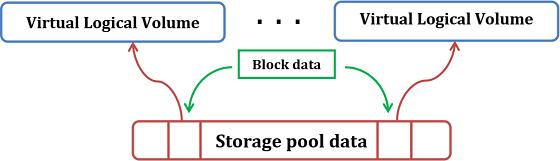
\includegraphics[width=8cm]{02_klyga_fig1}
  \caption{Двухуровневая модель}
  \label{02:klyga:fig1}
\end{figure}
\end{center} 

Распределением блоков для хранения данных из общего пула между виртуальными логическими томами управляет программа-менеджер. В случае необходимости новые блоки для хранения данных добавляются в общий пул, и в автоматическом режиме распределяются между виртуальными логическими томами, исключая необходимость проводить дополнительные манипуляции с ними (например, изменения размера файловой системы). При этом реальный размер каждого виртуального логического томам может превосходить суммарный объем общего пула хранения данных.

В ядре Linux абстракции виртуальных блочных устройств реализуются с помощью модуля «Device mapper» \cite{bib2}, а начиная с версии ядра 3.2 в него добавлена поддержка динамического выделения места в хранилище данных (thin provisioning) с возможностью реализации двухуровневой модели хранения данных.

При создании СХД с использование томов с «тонкой» настройкой (thin provisioning) \cite{bib3} на базе дистрибутива Linux необходимо учитывать версию ядра, возможности поддержки требуемого функционала с помощью дополнительных модулей, и  расширения общего пула хранения данных с учетом возрастающих потребностей.

Типовая структурная схема включает в себя два основных компонента: пул устройств (или том с ``тонкой'' настройкой thin pool) объединяющий вместе том метаданных (meta pool) и том данных (data pool)  и виртуальные тома (virtual volume) для пространства пользователя. В случае использования менеджера логических томов LVM2 \cite{bib4}, создание пулов томов с ``тонкой'' настройкой (thin pool) осуществляется в пределах одной Volume Group (VG) (рисунок \ref{02:klyga:fig2}).

\begin{center}
\begin{figure}[h!]
  \centering
  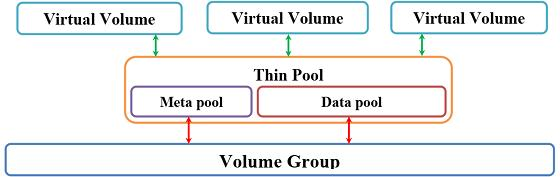
\includegraphics[width=9cm]{02_klyga_fig2}
  \caption{Типовая структурная схема СХД с томами ``тонкой'' настройки}
  \label{02:klyga:fig2}
\end{figure}
\end{center} 

При этом несмотря на это ограничение использование LVM2 более предпочтительно так как позволяет использовать дополнительные возможности:

\begin{itemize}
  \item подключение внешнего хранилища, доступного в режиме только для чтения в качестве основы для создания типовых LVM-разделов, при котором все обращения на чтение не изменённых данных прозрачно транслируются к базовому эталонному хранилищу, а все изменённые или новые данные обрабатываются в отдельном слое в режиме чтения-записи;
  \item поддержку динамической агрегации метаданных при помощи демона lvmetad;
  \item поддержку технологии LVM Cache для общих пулов хранения данных;
  \item работы со снапшотами.
\end{itemize}

Перед созданием СХД необходимо определить  параметры каждого виртуального тома, их суммарный общий объем (переменная \verb!$data_dev_size_max!), текущий доступный объем  для тома данных (переменная \verb!$data_dev_size!), возможность использования дополнительных накопителей для тома с метаданными (включая возможность резервирования), выбрать программу-менеджер для управления и используя формулы приведенные ниже определить значения ключевых переменных, при этом, для утилиты \verb!dmsetup! модуля «Device mapper» все значения указываются в количестве блоков, для LVM2 в байтах или других представлениях единиц измерений.

\subsection*{Размер виртуальных томов (virtual volume)}

Размер виртуальных томов (virtual volume) для пространства пользователей определяет администратор на основании технического задания или иных предпочтений, однако, при этом суммарный размер виртуальных томов не должен превышать предельно допустимые физические параметры системы  хранения данных в целом, в случае необходимости  должна быть реализована возможность их расширения с учетом возрастающих потребностей.

\subsection*{Размер фрагмента выделения (chunk size)}

\verb!$data_block_size=$dev_min_block_size * $count_block!, \\ где
\verb!$dev_min_block_size! – минимальный размер блока данных на устройстве, как правило, это значение равно 512 байт.
\verb!$count_block! – количество блоков данных которые можно использовать при раздаче, как правило от 128 до 2097152 для обычных томов данных, для сложной структуры 128, для снапшотов от 8 до 1048576.

\subsection*{Размер тома с метаданными}

\noindent{\small\verb!$metadata_dev_size = 48 * $data_dev_size_max / $data_block_size!}, \\где
\verb!$data_dev_size_max!  –  полный размер тома данных;\\
\verb!$data_block_size! – размер фрагмента выделения. 
При этом необходимо учитывать, что размер тома для хранения метаданных не может быть меньше 2Мб, и больше 16Гб, рекомендуемое значение по умолчанию 1Гб. Если по итогам расчетов размер тома для хранения метаданных превышает значение 16Гб, рекомендуется создавать несколько пулов хранения данных.

К размещению метаданных тонких томов стоит относится аккуратно, так  как, если данное пространство будет исчерпано, то пул будет выдавать ошибки ввода-вывода до тех пор, пока пул не будет переведен в автономный режим, и не будет выполнено восстановление для устранения потенциальных несоответствий. Поэтому, рекомендуется для пространства метаданных использовать отдельное выделенное устройство или несколько устройств с возможностью резервирования (например, объединить их в raid 1), а для повышения производительности использовать твердотельные накопители.

\subsection*{Определение значения переменной \\ \$low\_water\_mark}

{\small\verb!$low_water_mark = $count_block_sign_error * $data_block_size!},
\\ \verb!$count_block_sign_error! — значение количества свободных блоков в пуле данных при достижении которого выдать сигнал об исчерпании места;
\verb!$data_block_size! — текущее значение размера блока распределения.

Значение переменной \verb!$count_block_sign_error! определяется \linebreak системным администратором исходя из размера пула и критичности его оперативного расширения. 

Значение переменной \verb!$low_water_mark! используется для генерации однократного сигнала предупреждения при достижении низкого уровня свободного места в пуле хранения данных.

После выполнения расчета и анализа результатов, если необходимо провести корректировку значения \verb!$data_dev_size!, определить устройства для хранения данных и метаданных и выполнить первичную сборку и настройку СХД.

Пример расчета:

Условие:
Необходимо создать хранилище данных для 100 виртуальных машин с томами размером по 50GB для каждой, при наличии физического дискового пространства в 200GB и одного накопителя sdd емкостью 128GB.

\begin{enumerate}
  \item Определим значение переменной \verb!$data_dev_size_max!:\\
\verb!$data_dev_size_max!=100*50*1073741824=5 368 709 120 000 \linebreak байт
  \item Определим значение переменной \verb!$data_dev_size!, установив его в 98\% от максимально возможного (\textbf{рекомендовано}): 
\verb!$data_dev_size!=(200*1073741824)*0.98=210 453 397 504 байт
  \item Определим размер фрагмента выделения значением по умолчанию в 128 блоков по 512 байт:\\
 \verb!$data_block_size! = 128 * 512 =65 536 байт
  \item Определим размер тома для хранения метаданных:\\
 \verb!$metadata_dev_size! = 48 * 5 368 709 120 000/65 536 = \\ 3 932 160 000 байт или примерно 3,67GB
  \item Повторим предыдущие два вычисления, изменив исходные \linebreak данные.
Определим размер фрагмента выделения значением в 256 блоков по 512 байт:
 \verb!$data_block_size! = 256 * 512 = \linebreak 131 072 байт.
Определим размер тома для хранения метаданных:
 \verb!$metadata_dev_size! = 48 * 5 368 709 120 000/131 072 = \linebreak 1 966 080 000 байт или примерно 1,83GB
 Как видно, чем больше размер фрагмента выделения, тем меньше будет необходим том для хранения метаданных.
  \item Определим значения переменной \verb!$low_water_mark!, установив, ее значение равной 1024 блока: 
 \verb!$low_water_mark! = 1024 * 131 072 = 134 217 728 байт или примерно 128МБ
 Если это значение критично, то может его увеличить, например до 65 536 блоков:
 \verb!$low_water_mark! =  65 536 * 131 072 = 8 589 934 592 байт или примерно 8ГБ.
  \item Сопоставим полученные результаты с исходными данными и выберем  оптимальный вариант для создания пула с ``тонкой'' настройкой.
\end{enumerate}

\begin{thebibliography}{9}
\bibitem{bib1} {Thin provisioning \url{https://en.wikipedia.org/wiki/Thin_provisioning}}
\bibitem{bib2} {Device mapper \url{https://www.sourceware.org/dm}}
\bibitem{bib3} {Documentation kernel.org \url{https://www.kernel.org/doc/Documentation/device-mapper/thin-provisioning.txt}}
\bibitem{bib4} {Logical Volume Manager 2 (LVM2) \url{https://www.sourceware.org/lvm2/}}\end{thebibliography}
\end{document}

\documentclass[10pt, a5paper]{article}
\usepackage{pdfpages}
\usepackage{parallel}
\usepackage[T2A]{fontenc}
\usepackage{ucs}
\usepackage[utf8x]{inputenc}
\usepackage[polish,english,russian]{babel}
\usepackage{hyperref}
\usepackage{rotating}
\usepackage[inner=2cm,top=1.8cm,outer=2cm,bottom=2.3cm,nohead]{geometry}
\usepackage{listings}
\usepackage{graphicx}
\usepackage{wrapfig}
\usepackage{longtable}
\usepackage{indentfirst}
\usepackage{array}
\newcolumntype{P}[1]{>{\raggedright\arraybackslash}p{#1}}
\frenchspacing
\usepackage{fixltx2e} %text sub- and superscripts
\usepackage{icomma} % коскі ў матэматычным рэжыме
\PreloadUnicodePage{4}

\newcommand{\longpage}{\enlargethispage{\baselineskip}}
\newcommand{\shortpage}{\enlargethispage{-\baselineskip}}

\def\switchlang#1{\expandafter\csname switchlang#1\endcsname}
\def\switchlangbe{
\let\saverefname=\refname%
\def\refname{Літаратура}%
\def\figurename{Іл.}%
}
\def\switchlangen{
\let\saverefname=\refname%
\def\refname{References}%
\def\figurename{Fig.}%
}
\def\switchlangru{
\let\saverefname=\refname%
\let\savefigurename=\figurename%
\def\refname{Литература}%
\def\figurename{Рис.}%
}

\hyphenation{admi-ni-stra-tive}
\hyphenation{ex-pe-ri-ence}
\hyphenation{fle-xi-bi-li-ty}
\hyphenation{Py-thon}
\hyphenation{ma-the-ma-ti-cal}
\hyphenation{re-ported}
\hyphenation{imp-le-menta-tions}
\hyphenation{pro-vides}
\hyphenation{en-gi-neering}
\hyphenation{com-pa-ti-bi-li-ty}
\hyphenation{im-pos-sible}
\hyphenation{desk-top}
\hyphenation{elec-tro-nic}
\hyphenation{com-pa-ny}
\hyphenation{de-ve-lop-ment}
\hyphenation{de-ve-loping}
\hyphenation{de-ve-lop}
\hyphenation{da-ta-ba-se}
\hyphenation{plat-forms}
\hyphenation{or-ga-ni-za-tion}
\hyphenation{pro-gramming}
\hyphenation{in-stru-ments}
\hyphenation{Li-nux}
\hyphenation{sour-ce}
\hyphenation{en-vi-ron-ment}
\hyphenation{Te-le-pathy}
\hyphenation{Li-nux-ov-ka}
\hyphenation{Open-BSD}
\hyphenation{Free-BSD}
\hyphenation{men-ti-on-ed}
\hyphenation{app-li-ca-tion}

\def\progref!#1!{\texttt{#1}}
\renewcommand{\arraystretch}{2} %Іначай формулы ў матрыцы зліпаюцца з лініямі
\usepackage{array}

\def\interview #1 (#2), #3, #4, #5\par{

\section[#1, #3, #4]{#1 -- #3, #4}
\def\qname{LVEE}
\def\aname{#1}
\def\q ##1\par{{\noindent \bf \qname: ##1 }\par}
\def\a{{\noindent \bf \aname: } \def\qname{L}\def\aname{#2}}
}

\def\interview* #1 (#2), #3, #4, #5\par{

\section*{#1\\{\small\rm #3, #4. #5}}

\def\qname{LVEE}
\def\aname{#1}
\def\q ##1\par{{\noindent \bf \qname: ##1 }\par}
\def\a{{\noindent \bf \aname: } \def\qname{L}\def\aname{#2}}
}

\switchlang{ru}
\begin{document}
\title{Modern strace}
\author{Dmitry Levin, Moscow, Russian Federation\footnote{\url{ldv@altlinux.org}, \url{http://lvee.org/ru/abstracts/227}}}
\maketitle
\begin{abstract}
strace is a diagnostic, debugging and instructional utility for\linebreak Linux. It is used to monitor and tamper with interactions between processes and the Linux kernel, which include system calls, signal deliveries, and changes of process state. Linux developers are usually aware of strace and use it occasionally, but their know\-ledge about modern strace features is often quite limited. Here the maintainer of strace describes features of modern strace and demonstrates what kinds of problems they help to solve.
\end{abstract}
\subsection*{Введение} 
strace как инструмент мониторинга взаимодействия пользовательских процессов с ядром существует уже почти 28 лет и широко применяется для диагностики, отладки и изучения поведения ПО. Многочисленные параметры управления фильтрацией дают возможность пользователю strace легко и гибко настраивать отображение системных вызовов и сигналов. С каждым выпуском strace таких возможностей становится больше, а точность отображения --- выше.

Начиная с версии 4.13, выпущенной в июле 2016 года, расписание выпусков новых версий strace синхронизировано с расписанием выпусков новых версий ядра linux. Таким образом новые интерфейсы, добавляемые в релизы ядра linux, сопровождаются соответствующими парсерами, добавляемыми в релизы strace.

strace относится к традиционным инструментам, и пользователи со стажем зачастую не подозревают о новых возможностях, появившихся в strace за последние несколько лет, таких как 
\begin{itemize} 
\item отслеживание файловых путей: параметр \texttt{-y}; 
\item отслеживание сетевых протоколов: параметр \texttt{-yy}; 
\item отслеживание стека вызовов: параметр \texttt{-k}; 
\item сбор статистики по времени, проведённому отслеживаемыми процессами в системных вызовах: параметр \texttt{-w}; 
\item фильтрация системных вызовов по файловым путям: параметр \texttt{-P}; 
\item фильтрация системных вызовов по именам: с помощью регулярных выражений и новых классов системных вызовов; 
\item модификация системных вызовов: инъекции ошибок, кодов возврата, сигналов, и задержек. 
\end{itemize}

\subsection*{Отслеживание файловых путей и фильтрация по файловым путям}

Начиная с версии 4.7, выпущенной в мае 2012 года, реализована возможность отслеживания файловых путей, соответствующих дескрипторам, с помощью параметра \texttt{-y}.

В той же версии была реализована возможность фильтрации системных вызовов по файловым путям, соответствующим аргументам системных вызовов и файловым дескрипторам, с помощью параметра \texttt{-P}.

\subsection*{Отслеживание сетевых протоколов и устройств}

Начиная с версии 4.10, выпущенной в марте 2015 года, реализована возможность отслеживания характеристик сетевых протоколов, соответствующих дескрипторам сокетов, с помощью параметра \texttt{-yy}.

Начиная с версии 4.22, выпущенной в апреле этого года, с помощью этого же параметра можно отслеживать и характеристики устройств.

\subsection*{Отслеживание стека вызовов}

Начиная с версии 4.9, выпущенной в августе 2014 года, реализована экспериментальная возможность отслеживания стека вызовов функций с помощью параметра \texttt{-k}. Начиная с версии 4.23, выпущенной в июне этого года, усовершенствованная реализация этой возможности с использованием библиотеки libdw уже не носит экспериментальный статус.

\subsection*{Cбор статистики} 
Начиная с версии 4.9, выпущенной в августе 2014 года, реализована возможность сбора статистики по времени, проведённому отслеживаемыми процессами в системных вызовах, с помощью параметра \texttt{-w}.

\subsection*{Фильтрация системных вызовов по именам} 
Начиная с версии 4.17, выпущенной в мае 2017 года, синтаксис описания множества системных вызовов существенно расширился.

В описании имён системных вызовов теперь поддерживаются регулярные выражения:

\texttt{strace \textbf{-e trace}=/\textit{regexp}}.

В описании множества системных вызовов поддерживаются описания, которым не соответствует ни одного системного вызова:

\texttt{strace \textbf{-e trace}=?\textit{set}}.

Имена классов системных вызовов теперь начинаются с префикса \texttt{\%}:

\texttt{strace \textbf{-e trace}=\%\textit{class}}.

Прежний способ именования классов без префикса \texttt{\%} поддерживается, но уже считается устаревшим и не рекомендуется для применения.

Добавлены новые классы системных вызовов семейства stat: 
\%\texttt{stat}, 
\%\texttt{lstat}, 
\%\texttt{fstat}, 
\%\%\texttt{stat}, 
\%\texttt{statfs}, 
\%\texttt{fstatfs}, 
\%\%\texttt{statfs}.

\subsection*{Модификация системных вызовов} 
Начиная с версии 4.15, выпущенной в декабре 2016 года, реализован механизм инъекций ошибок в системные вызовы. 
Синтаксис syscall fault injection выглядит следующим образом:

\texttt{strace \textbf{-e fault}=\textit{set}[:\textbf{error}=\textit{errno}][:\textbf{when}=\textit{expr}]}

Начиная с версии 4.16, выпущенной в феврале 2017 года, реализован более общий механизм вмешательства в системные вызовы, который, помимо инъекций ошибок, позволяет осуществлять инъекции кодов возврата и сигналов, а начиная с версии 4.22, выпущенной в апреле 2018 года, ещё и инъекции задержек. 
Интерфейс этого нового механизма выглядит следующим образом:

\texttt{strace \textbf{-e inject}=\textit{set}[parameters]}

где \texttt{parameters} могут принимать следующие значения: 
\begin{itemize} 
\item \texttt{:\textbf{error}=\textit{errno}} либо \texttt{:\textbf{retval}=\textit{value}} -- 
инъекция ошибки либо кода возврата; 
\item \texttt{:\textbf{syscall}=\textit{syscall}} -- 
подменяемый системный вызов для инъекции ошибок либо кода возврата; 
\item \texttt{:\textbf{signal}=\textit{sig}} -- 
инъекция сигнала; 
\item \texttt{:\textbf{delay\_enter}=\textit{usecs}} -- 
инъекция задержки перед системным вызовом; 
\item \texttt{:\textbf{delay\_exit}=\textit{usecs}} -- 
инъекция задержки после системного вызова; 
\item \texttt{:\textbf{when}=\textit{expr}} -- 
правило применения инъекции. 
\end{itemize}

Пример инъекции ошибки:

 
\lstset{
  basicstyle=\ttfamily,
  columns=fullflexible,
  breaklines=true,
  postbreak=\mbox{\textcolor{red}{$\hookrightarrow$}\space},
}
\begin{lstlisting}[language=bash]
$ strace -e trace=/open -e inject=/open:when=3:error=EACCES cat /dev/null 
openat(AT_FDCWD, "/etc/ld.so.cache", O_RDONLY|O_CLOEXEC) = 3 
openat(AT_FDCWD, "/lib64/libc.so.6", O_RDONLY|O_CLOEXEC) = 3 
openat(AT_FDCWD, "/dev/null", O_RDONLY) = -1 EACCES (Permission denied) (INJECTED) 
cat: /dev/null: Permission denied 
+++ exited with 1 +++ 
\end{lstlisting}

Пример инъекции задержки:

\begin{lstlisting}[language=bash]
$ dd if=/dev/zero of=/dev/null bs=1M count=10 
10+0 records in 
10+0 records out 
10485760 bytes (10 MB, 10 MiB) copied, 0.00211354 s, 
5.0 GB/s

$ strace -e inject=write:delay_exit=100000 -e write -o /dev/null \ 
dd if=/dev/zero of=/dev/null bs=1M count=10 
10+0 records in 
10+0 records out 
10485760 bytes (10 MB, 10 MiB) copied, 1.10658 s, 
9.5 MB/s 
\end{lstlisting}
\end{document}

\documentclass[10pt, a5paper]{article}
\usepackage{pdfpages}
\usepackage{parallel}
\usepackage[T2A]{fontenc}
\usepackage{ucs}
\usepackage[utf8x]{inputenc}
\usepackage[polish,english,russian]{babel}
\usepackage{hyperref}
\usepackage{rotating}
\usepackage[inner=2cm,top=1.8cm,outer=2cm,bottom=2.3cm,nohead]{geometry}
\usepackage{listings}
\usepackage{graphicx}
\usepackage{wrapfig}
\usepackage{longtable}
\usepackage{indentfirst}
\usepackage{array}
\newcolumntype{P}[1]{>{\raggedright\arraybackslash}p{#1}}
\frenchspacing
\usepackage{fixltx2e} %text sub- and superscripts
\usepackage{icomma} % коскі ў матэматычным рэжыме
\PreloadUnicodePage{4}

\newcommand{\longpage}{\enlargethispage{\baselineskip}}
\newcommand{\shortpage}{\enlargethispage{-\baselineskip}}

\def\switchlang#1{\expandafter\csname switchlang#1\endcsname}
\def\switchlangbe{
\let\saverefname=\refname%
\def\refname{Літаратура}%
\def\figurename{Іл.}%
}
\def\switchlangen{
\let\saverefname=\refname%
\def\refname{References}%
\def\figurename{Fig.}%
}
\def\switchlangru{
\let\saverefname=\refname%
\let\savefigurename=\figurename%
\def\refname{Литература}%
\def\figurename{Рис.}%
}

\hyphenation{admi-ni-stra-tive}
\hyphenation{ex-pe-ri-ence}
\hyphenation{fle-xi-bi-li-ty}
\hyphenation{Py-thon}
\hyphenation{ma-the-ma-ti-cal}
\hyphenation{re-ported}
\hyphenation{imp-le-menta-tions}
\hyphenation{pro-vides}
\hyphenation{en-gi-neering}
\hyphenation{com-pa-ti-bi-li-ty}
\hyphenation{im-pos-sible}
\hyphenation{desk-top}
\hyphenation{elec-tro-nic}
\hyphenation{com-pa-ny}
\hyphenation{de-ve-lop-ment}
\hyphenation{de-ve-loping}
\hyphenation{de-ve-lop}
\hyphenation{da-ta-ba-se}
\hyphenation{plat-forms}
\hyphenation{or-ga-ni-za-tion}
\hyphenation{pro-gramming}
\hyphenation{in-stru-ments}
\hyphenation{Li-nux}
\hyphenation{sour-ce}
\hyphenation{en-vi-ron-ment}
\hyphenation{Te-le-pathy}
\hyphenation{Li-nux-ov-ka}
\hyphenation{Open-BSD}
\hyphenation{Free-BSD}
\hyphenation{men-ti-on-ed}
\hyphenation{app-li-ca-tion}

\def\progref!#1!{\texttt{#1}}
\renewcommand{\arraystretch}{2} %Іначай формулы ў матрыцы зліпаюцца з лініямі
\usepackage{array}

\def\interview #1 (#2), #3, #4, #5\par{

\section[#1, #3, #4]{#1 -- #3, #4}
\def\qname{LVEE}
\def\aname{#1}
\def\q ##1\par{{\noindent \bf \qname: ##1 }\par}
\def\a{{\noindent \bf \aname: } \def\qname{L}\def\aname{#2}}
}

\def\interview* #1 (#2), #3, #4, #5\par{

\section*{#1\\{\small\rm #3, #4. #5}}

\def\qname{LVEE}
\def\aname{#1}
\def\q ##1\par{{\noindent \bf \qname: ##1 }\par}
\def\a{{\noindent \bf \aname: } \def\qname{L}\def\aname{#2}}
}

\begin{document}
\title{ZFS на базе проекта «ZFS on Linux»}
\author{Александр Клыга, Minsk, Belarus\footnote{\url{alex_kls@mail.ru}, \url{https://lvee.org/en/abstracts/297}}}
\maketitle
\begin{abstract}
What is the project "openZFS"? It's concept evolution open source project "ZFS on Linux" in future.
\end{abstract}
\subsection*{Архитектура, лицензионные ограничения и перспективы развития файловой системы ZFS в рамках проекта openZFS}

ZFS (Zettabyte File System) \cite{bib1} — 128 битная файловая система была разработана двумя инженерами компании Sun Microsystems для хранения больших объемов данных (например, максимальный общим  объемом тома может достигать 256 зеттабайт), с использованием концепции динамического распределения блоков из общего хранилища. В ней используется модель объектных транзакций на основе механизма копирования при записи (Copy-On-Write COW), поддерживается проверка целостности информации с возможность автоматического восстановления, создание снимков, обеспечение отказоустойчивости с помощью технологии RAID-Z. В состав  ее компонентов  включен менеджер логических томов для управления виртуальными абстракциями пулов хранения данных на базе физических устройств, с возможностью облегченного администрирования с использованием интерфейса командной строки. Дополнительные возможности  определяются версией пула (ZFS Pool Version) и его реализацией в зависимости от дистрибутива операционной системы.

В 2006 году начаты работы по включению файловой системы ZFS в состав операционной системы (ОС) Linux, несмотря на проблемы лицензирования и архитектурной не совместимости ОС \linebreak Solaris и Linux.

\subsection*{Проблемы лицензионной совместимости  с платформой ОС Linux}

\begin{enumerate}
  \item Код ZFS распространяется под лицензией CDDL (Common Development and Distribution License), несовместимой с лицензией GPLv2 ядра Linux, что не дает возможность включения его в состав основной ветки ядра Linux, а изменение типа лицензии в силу исторических и иных причин уже невозможно.
  \item Официально все права на ZFS принадлежат компании Oracle, однако так как код ZFS распространяется под лицензией \linebreak CDDL, порты для других операционных систем и платформ могут производиться без участия Oracle, что дает возможность делать собственную разработку на базе исходного проекта.
\end{enumerate}

\subsection*{Решения проблемы лицензирования и реализации ZFS в ОС Linux}

Первым решением по поддержке ZFS в Linux стало разработка порта FUSE \cite{bib2}, данное решение было представлено в 2006 году и позволило реализовать локальную файловую систему хранения данных большой емкости в пространстве пользователя.

Вторым решением стала разработка нативного порта (native \linebreak port) для Linux, старт данному проекту был дан в 2008 году, а  возглавил его Брайан Белендорф вместе с сотрудниками Ливерморской национальной лаборатории. В  мае 2010 года, для обхода проблемы лицензирования он предложил метод реализации  ZFS для Linux в виде загружаемого модуля (под лицензией CDDL) поставляемого отдельно от ядра. При этом, что бы соответствовать требованиям лицензии GPLv2 модуль ZFS поставляется в виде исходных кодов и собирается в системе пользователя, например, с использованием DKMS (Dynamic Kernel Module Support) \cite{bib3}, непосредственно после установки пакета. Для дистрибутивов на базе RHEL/CentOS была добавлена возможность установки модуля ZFS в виде универсального kABI-tracking kmod пакета \cite{bib4}. В дальнейшим все наработки в данном направлении стали основой проекта “ZFS on Linux” (ZOL) \cite{bib5}.

В том же 2010 году было объявлено о закрытии проекта \linebreak OpenSolaris, что стало поводом для создания ответвления (форка) в рамках которого были продолжены работы по развитию открытой спецификации ZFS.

Первый стабильный релиз ZFS для Linux на базе ZOL был представлен в 2013 году, вместе с проектом openZFS \cite{bib6}, основной задачей которого ставили гарантировать дальнейшую эволюцию ZFS, сосредоточить разработку в рамках единого вектора развития и создания  кросс-платформенного решения, упрощающий использование ZFS в различных операционных системах.

Ключевым для развития ZFS на платформе Linux стал 2016 год, когда были опубликованы некоторые разъяснения по итогам анализа результатов  исследования юристов компании Canonical о в лицензионной совместимости модуля ZFS и ядра Linux на предмет возможности его использования в дистрибутиве \cite{bib7}. Несмотря на неоднозначные результаты и последующие дискуссии с правозащитной организацией Software Freedom Conservancy (SFC), сначала компания  компании Canonical включила модуль поддержки ZFS в состав своего дистрибутива Ubuntu, а затем разработчики Debian добавили его в репозитории проекта.

\subsection*{Решение проблемы архитектурной несовместимости ОС Solaris и Linux}

Архитектурно файловая система ZFS состоит их трех основных слоев:

\begin{itemize}
  \item \textbf{«Interface Layer» (IL), основные компоненты «ZFS \linebreak Emulated Volume» (ZVOL) и «ZFS POSIX Layer» (ZPL):}
  \item \textbf{«Transactional Object Layer» (TOL), основной компонент «Data Management Unit» (DMU);}
  \item \textbf{«Pooled Storage Layer» (PSL), основной компонент \linebreak «Storage Pool Allocator» (SPA).}
\end{itemize}

Четвертый компонент \textbf{Layered Driver Interface (LDI)} реализован только в ОС Solaris и представляет собой набор компонентов интерфейсов взаимодействия с физическими накопителями и реализации дополнительных функций обработки их отказов.

Поэтому в архитектуру ZFS (рисунок \ref{xx:klyga:fig1}) были внесены изменения и вместо LDI был добавлен новый слой получивших название \textbf{«Solaris Porting Layer» (SPL)} в  состав которого были включены реализации компонентов и вспомогательных утилит портированых из Solaris.

\begin{center}
\begin{figure}[h!]
  \centering
  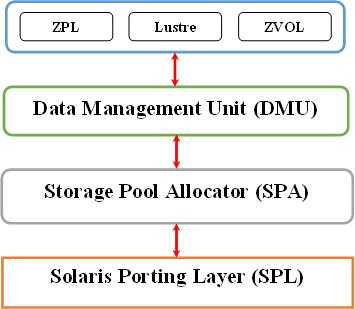
\includegraphics[width=8cm]{xx_klyga_arch_zfs}
  \caption{Архитектура ZFS для ОС Linux}
  \label{xx:klyga:fig1}
\end{figure}
\end{center}

Дополнительно был реализован еще один компонент IL включенный в состав ZFS в 2009 году ``Lustre'' позволяющий использовать ZFS в роли бэкенда для кластерных и сетевых файловых систем, например Lustre или pNFS (рисунок \ref{xx:klyga:fig2}).

\begin{center}
\begin{figure}[h!]
  \centering
  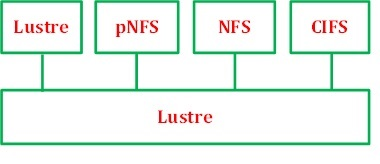
\includegraphics[width=8cm]{xx_klyga_zfs_lustre}
  \caption{Дополнительный компонент ``Lustre''}
  \label{xx:klyga:fig2}
\end{figure}
\end{center}

Использование данного компонента позволяет упростить интеграцию распределенных и сетевых файловых систем с ZFS, однако, при этом она остается локальной файловой системой.

\textbf{Возможности ZFS на базе проекта ``ZFS on Linux''}

Функциональные возможности ZFS на базе проекта “ZFS on Linux”:

\begin{itemize}
  \item режим multihost (MMP, Multi Modifier Protection);
  \item расширенная система квот;
  \item шифрование наборов данных;
  \item раздельный выбор классов распределения блоков (allocation classes);
  \item использование векторных процессорных инструкций для ускорения реализация RAIDZ и вычисления контрольных сумм;
  \item поддержку хранения контрольных сумм с использованием более надёжных криптографических хэшей SHA-512, Skein и Edon-R;
  \item защиту операций импорта пула в отказоусточивых конфигурациях;
  \item поддержка больших dnode для оптимизации работы с метаданными;
  \item дополнительные параметры (более 50) для тонкой настройки работы модуля ядра;
  \item улучшенный инструментарий командной строки.
\end{itemize}

Дополнительные возможности определяются версией модуля и ядра дистрибутива ОС Linux.

\subsection*{Дальнейшее развитие ZFS в рамках проекта \linebreak openZFS}

До конца 2017 года основной вклад в развитие ZFS вносил проект ``ZFS on Linux'' совместно с компанией  Delphix с использованием наработок основанных на оригинальном коде ZFS, импортированном из проекта OpenSolaris и расширенном улучшениями и исправлениями от сообщества Illumos.

Однако в 2018 году компания Delphix приняла решение о прекращении поддержки развития ZFS и переходе на использование кода проекта  ``ZFS on Linux'' \cite{bib8}, что привело к стагнации проекта Illumos.

В конце 2018 года о намерении перейти на проект ``ZFS on Linux'' объявила команда разработчиков FreeBSD \cite{bib9}. Таким образом вся активность по развитию и сопровождению проектов связанных с открытыми реализациями ZFS на базе проекта openZFS сократилась до одного ``ZFS on Linux''.

Новый релиз модуля ZFS для ядра Linux версии 0.8.0 был представлен 23 мая 2019 года, и включает в себя много изменений и дополнений \cite{bib10}. Однако, при этом необходимо учитывать, что реализация ZFS на базе проекта openZFS не обеспечивает полноценной совместимости с продуктами компании Oracle и развивается отдельно.

\begin{thebibliography}{9}
\bibitem{bib1} {ZFS in Wikipedia \url{https://ru.wikipedia.org/wiki/ZFS}}
\bibitem{bib2} {Модуль ядра FUSE \url{https://en.wikipedia.org/wiki/Filesystem_in_Userspace}}
\bibitem{bib3} {DKMS on GitHub \url{https://github.com/dell/dkms}}
\bibitem{bib4} {The ELRepo Blog. kABI-tracking kmod  \url{http://elrepoproject.blogspot.com/2016/02/kabi-tracking-kmod-packages.html}}
\bibitem{bib5} {ZFS on Linux \url{https://zfsonlinux.org/index.html}}
\bibitem{bib6} {Проект openZFS \url{http://open-zfs.org}}
\bibitem{bib7} {Dustin Kirkland. ZFS Licensing and Linux \url{http://blog.dustinkirkland.com/2016/02/zfs-licensing-and-linux.html}}
\bibitem{bib8} {Delphix Blog. Kickoff to The Future \url{https://www.delphix.com/blog/kickoff-future-eko-2018}}
\bibitem{bib9} {The future of ZFS in FreeBSD \url{https://lists.freebsd.org/pipermail/freebsd-current/2018-December/072422.html}}
\bibitem{bib10} {ZFS on Linux. Release zfs-0.8.0 \url{https://github.com/zfsonlinux/zfs/releases}}\end{thebibliography}
\end{document}

\documentclass[10pt, a5paper]{article}
\usepackage{pdfpages}
\usepackage{parallel}
\usepackage[T2A]{fontenc}
\usepackage{ucs}
\usepackage[utf8x]{inputenc}
\usepackage[polish,english,russian]{babel}
\usepackage{hyperref}
\usepackage{rotating}
\usepackage[inner=2cm,top=1.8cm,outer=2cm,bottom=2.3cm,nohead]{geometry}
\usepackage{listings}
\usepackage{graphicx}
\usepackage{wrapfig}
\usepackage{longtable}
\usepackage{indentfirst}
\usepackage{array}
\newcolumntype{P}[1]{>{\raggedright\arraybackslash}p{#1}}
\frenchspacing
\usepackage{fixltx2e} %text sub- and superscripts
\usepackage{icomma} % коскі ў матэматычным рэжыме
\PreloadUnicodePage{4}

\newcommand{\longpage}{\enlargethispage{\baselineskip}}
\newcommand{\shortpage}{\enlargethispage{-\baselineskip}}

\def\switchlang#1{\expandafter\csname switchlang#1\endcsname}
\def\switchlangbe{
\let\saverefname=\refname%
\def\refname{Літаратура}%
\def\figurename{Іл.}%
}
\def\switchlangen{
\let\saverefname=\refname%
\def\refname{References}%
\def\figurename{Fig.}%
}
\def\switchlangru{
\let\saverefname=\refname%
\let\savefigurename=\figurename%
\def\refname{Литература}%
\def\figurename{Рис.}%
}

\hyphenation{admi-ni-stra-tive}
\hyphenation{ex-pe-ri-ence}
\hyphenation{fle-xi-bi-li-ty}
\hyphenation{Py-thon}
\hyphenation{ma-the-ma-ti-cal}
\hyphenation{re-ported}
\hyphenation{imp-le-menta-tions}
\hyphenation{pro-vides}
\hyphenation{en-gi-neering}
\hyphenation{com-pa-ti-bi-li-ty}
\hyphenation{im-pos-sible}
\hyphenation{desk-top}
\hyphenation{elec-tro-nic}
\hyphenation{com-pa-ny}
\hyphenation{de-ve-lop-ment}
\hyphenation{de-ve-loping}
\hyphenation{de-ve-lop}
\hyphenation{da-ta-ba-se}
\hyphenation{plat-forms}
\hyphenation{or-ga-ni-za-tion}
\hyphenation{pro-gramming}
\hyphenation{in-stru-ments}
\hyphenation{Li-nux}
\hyphenation{sour-ce}
\hyphenation{en-vi-ron-ment}
\hyphenation{Te-le-pathy}
\hyphenation{Li-nux-ov-ka}
\hyphenation{Open-BSD}
\hyphenation{Free-BSD}
\hyphenation{men-ti-on-ed}
\hyphenation{app-li-ca-tion}

\def\progref!#1!{\texttt{#1}}
\renewcommand{\arraystretch}{2} %Іначай формулы ў матрыцы зліпаюцца з лініямі
\usepackage{array}

\def\interview #1 (#2), #3, #4, #5\par{

\section[#1, #3, #4]{#1 -- #3, #4}
\def\qname{LVEE}
\def\aname{#1}
\def\q ##1\par{{\noindent \bf \qname: ##1 }\par}
\def\a{{\noindent \bf \aname: } \def\qname{L}\def\aname{#2}}
}

\def\interview* #1 (#2), #3, #4, #5\par{

\section*{#1\\{\small\rm #3, #4. #5}}

\def\qname{LVEE}
\def\aname{#1}
\def\q ##1\par{{\noindent \bf \qname: ##1 }\par}
\def\a{{\noindent \bf \aname: } \def\qname{L}\def\aname{#2}}
}

\switchlang{en}
\begin{document}
\title{Free software porting on the Elbrus architecture}
\author{Andrew Savchenko, Moscow, Russian Federation\footnote{\url{bircoph@gmail.com}, \url{http://lvee.org/ru/abstracts/303}}}
\maketitle
\begin{abstract}
The Elbrus (aka E2000, aka E2K) is the unique Russian VLIW CPU with its own architecture, instruction set and security fea\-tures. In this talk we'll discuss main architecture features interes\-ting for general software developers, particularities of the system compiler and main obstacles during software porting. Interaction with various free software upstreams will be discussed as well.
\end{abstract}
Unlike most other CPUs available the Elbrus family (E2K) uses a VLIW instruction set (Very Large Instruction Word) and features 25 general instructions per cycle. Such dependency puts much more demands on the system compiler for optimization. Furthermore in order to minimize the silicone usage every high level function possible was moved from the hardware to the compiler, so roughly speaking there is no microcode and microcode-level operations are done during a compile time, not run-time like on x86 family of CPUs.

While such approach yields better power usage and performance per number of transistors used, it's side effect is that the only system compiler — the LCC — is closed source and will likely stay that way. The LCC tries to mimic GCC by user interface (both supported options and GCC-specific features) but here similarity ends. The LCC is based on EDG\cite{Savchenko1} frontend and MCST-made multi-layer backend.

However, free software is also used in the compiler toolchain: \\libstdc++, libatomic, libgcc\_s, the C runtime and so on. It was a challenging task to separate all free components from the compiler bundle, build them from the source and package them apart from binary blobs left to form fully functional toolchain meeting the distribution standards (ALT in our case).

While the Elbrus machine supports running x86 and amd64 instruc- tions using run-time JIT compiler for x86/amd64 assembly, we do not use this mode for both performance and security reasons. This JIT compiler is left for special purposes like running proprietary closed source software without native E2K support.

Most software porting problems rise from the lack of full compatibility with GCC due to various reasons. The main problem is that the EDG frontend — which is responsible for parsing program's syntax — lags behind the GCC in supported language features, e.g. current production version lcc-1.23 is on par with gcc-5.5. So many code needs backporting to older C++ standard or similar tweaks in order to build on the E2K.

However, there are other cases as well:

\begin{itemize}
  \item Sometimes the LCC notices problem which GCC skips like \newline uninitialized variable usage. This causes problem especially in combination with -Werror. Sometimes we fix such problems, some- times we just disable -Werror.
  \item lcc-1.23 implements not all extended data types from gcc-5.5, e.g. \_\_(u)int128\_t and \_Decimal64. Such problems are usually easily solved by macro definitions.
  \item Not all GCC builtins are implemented, some may never be.
  \item LCC's preprocessor assumes input to be C/C++ code and replaces indentation tabs with spaces. This breaks applications which use a compiler's preprocessor to parse Makefiles and similar tabulation sensitive data.
  \item Some software depends on tricky GCC features, e.g. on \\undocumented VLAIS (variable length array in structure) or on writing C++ code <<careful enough>> to not to use C++ runtime and to link such code as normal C code. While such tricks work with gcc, they create many problems with other compilers, sample case is libgraphite2.  Such problems are solved on case-by-case basis and prone to be painful issues.
\end{itemize}

For now the LCC supports only C, C++ and Fortran. So it is not possible to build and use on the E2K in native mode software written in languages with their own code generators like Go, Rust and Haskell. This problem should be solved with ongoing effort to create an LLVM backend for the LCC, but ETA is unknown.

Aside from compiler induced issues the E2K has significantly different hardware architecture besides using VLIW. It feature three independent stacks: for data, for function pointers and for function arguments. This way a system is hardware protected from many kinds of buffer overflow and pointer hijacking attacks. But there is price to pay: low-level memory manipulations like garbage collectors or context switching should be rewritten to take into account this stack layout.

Of course system calls and ioctls are also partly different and such difference should be taken into account while porting software using these calls directly. But this is the common rule for all new architectures.

The E2K also supports a tagged memory, but we do not use this mode to build general purpose applications since drastic changes are required to work in strict security environment, e.g. all virtual calls in C++ will be invalidated by design. More details on the E2K hardware architecture and security features may be learned from the MCST official textbook\cite{Savchenko2}.

Upstreaming software for the Elbrus has its limitations, but is \\possible. The main obstacle is that both hardware and software are distributed by MCST under NDA for now, thus we cannot publish patches received from them without prior approval. However, we are free to upstream all own code including low-level stuff and assembly. And the ALT team already upstreamed E2K-specific changes to many free software projects like ruby, lxc, gimagereader, imake. More complete list is available at our wiki\cite{Savchenko3}.

All people are different, upstreams are different as well. Some gladly accept patches, some are not interested and ignore changes, some \\demand the toolchain to be opened before accepting any changes. With some luck NDA restrictions may be mostly lifted in the future and this beautiful architecture will see a second wind in its development.

\begin{thebibliography}{99}
\bibitem{Savchenko1}\url{https://www.edg.com/}
\bibitem{Savchenko2}\url{http://www.mcst.ru/files/511cea/886487/1a8f40/000000/book\_elbrus.pdf}
\bibitem{Savchenko3}\url{https://www.altlinux.org/Эльбрус/upstream}
\end{thebibliography}
\end{document}

\documentclass[10pt, a5paper]{article}
\usepackage{pdfpages}
\usepackage{parallel}
\usepackage[T2A]{fontenc}
\usepackage{ucs}
\usepackage[utf8x]{inputenc}
\usepackage[polish,english,russian]{babel}
\usepackage{hyperref}
\usepackage{rotating}
\usepackage[inner=2cm,top=1.8cm,outer=2cm,bottom=2.3cm,nohead]{geometry}
\usepackage{listings}
\usepackage{graphicx}
\usepackage{wrapfig}
\usepackage{longtable}
\usepackage{indentfirst}
\usepackage{array}
\newcolumntype{P}[1]{>{\raggedright\arraybackslash}p{#1}}
\frenchspacing
\usepackage{fixltx2e} %text sub- and superscripts
\usepackage{icomma} % коскі ў матэматычным рэжыме
\PreloadUnicodePage{4}

\newcommand{\longpage}{\enlargethispage{\baselineskip}}
\newcommand{\shortpage}{\enlargethispage{-\baselineskip}}

\def\switchlang#1{\expandafter\csname switchlang#1\endcsname}
\def\switchlangbe{
\let\saverefname=\refname%
\def\refname{Літаратура}%
\def\figurename{Іл.}%
}
\def\switchlangen{
\let\saverefname=\refname%
\def\refname{References}%
\def\figurename{Fig.}%
}
\def\switchlangru{
\let\saverefname=\refname%
\let\savefigurename=\figurename%
\def\refname{Литература}%
\def\figurename{Рис.}%
}

\hyphenation{admi-ni-stra-tive}
\hyphenation{ex-pe-ri-ence}
\hyphenation{fle-xi-bi-li-ty}
\hyphenation{Py-thon}
\hyphenation{ma-the-ma-ti-cal}
\hyphenation{re-ported}
\hyphenation{imp-le-menta-tions}
\hyphenation{pro-vides}
\hyphenation{en-gi-neering}
\hyphenation{com-pa-ti-bi-li-ty}
\hyphenation{im-pos-sible}
\hyphenation{desk-top}
\hyphenation{elec-tro-nic}
\hyphenation{com-pa-ny}
\hyphenation{de-ve-lop-ment}
\hyphenation{de-ve-loping}
\hyphenation{de-ve-lop}
\hyphenation{da-ta-ba-se}
\hyphenation{plat-forms}
\hyphenation{or-ga-ni-za-tion}
\hyphenation{pro-gramming}
\hyphenation{in-stru-ments}
\hyphenation{Li-nux}
\hyphenation{sour-ce}
\hyphenation{en-vi-ron-ment}
\hyphenation{Te-le-pathy}
\hyphenation{Li-nux-ov-ka}
\hyphenation{Open-BSD}
\hyphenation{Free-BSD}
\hyphenation{men-ti-on-ed}
\hyphenation{app-li-ca-tion}

\def\progref!#1!{\texttt{#1}}
\renewcommand{\arraystretch}{2} %Іначай формулы ў матрыцы зліпаюцца з лініямі
\usepackage{array}

\def\interview #1 (#2), #3, #4, #5\par{

\section[#1, #3, #4]{#1 -- #3, #4}
\def\qname{LVEE}
\def\aname{#1}
\def\q ##1\par{{\noindent \bf \qname: ##1 }\par}
\def\a{{\noindent \bf \aname: } \def\qname{L}\def\aname{#2}}
}

\def\interview* #1 (#2), #3, #4, #5\par{

\section*{#1\\{\small\rm #3, #4. #5}}

\def\qname{LVEE}
\def\aname{#1}
\def\q ##1\par{{\noindent \bf \qname: ##1 }\par}
\def\a{{\noindent \bf \aname: } \def\qname{L}\def\aname{#2}}
}

\switchlang{ru}
\begin{document}
\title{Buildroot: опыт создания прошивок архитектуры ARM для мониторинга}
\author{Алексей Лукьянчук, Москва, Russian Federation\footnote{\url{skif@skif-web.ru}, \url {https://lvee.org/ru/abstracts/310}}}
\maketitle
\begin{abstract}
Using the Buildroot build system allows to create customized solutions that can be operated by personnel with minimal know\-ledge of the Linux operating systems. This system is friendly to beginners, but at the same time gives ample opportunities for customization for an experienced developer. It is perfect for solving the problem of inexpensive, but full-featured monitoring of it infrastructure, minimally demanding to the training of its operating personnel.
\end{abstract}
Небольшие по размеру фирмы с одной стороны, нуждаются в качественном мониторинге своей инфраструктуры(особенно в свете повсеместной виртуализации), с другой стороны, для них финансово тяжело закупать новое оборудование под мониторинг и содержать достаточно квалифицированный ИТ-персонал. 

Как правило, в таких организациях работает 1 системный администратор, знающий ОС семейства Windows и слабо знакомый с Zabbix, Linux.

Для решения данной задачи подходит связка Buildroot + одноплатный компьютер архитектуры  ARM + Zabbix.

Прежде всего, не следует путать систему сборки и дистрибутив. Buildroot может собрать систему из набора пакетов, которые ему предложили. Buildroot построен на make-файлах и поэтому имеет огромные возможности по кастомизации. 

Первоначальное конфигурирование системы можно провести через KConfig. Выбрать целевую архитектуру, настроить загрузчик, добавить нужные пакеты. Отдельно сконфигурировать ядро. Для многих плат, а так же qemu с эмуляцией разных архитектур, уже есть defconfig’и конфигураций. Собираем настроенную систему и получаем работающий дистрибутив.

Buildroot хорош своей кастомизацией. В данном случае я портирую пакет Zabbix для сборки из исходников. Кроме того, описание пакета, настройки системы в целом, а также дополнительные файлы будут храниться в отдельном оверлее, который легко передавать другим разработчикам. Для этого используется механизм External-tree.

Для портирования пакета нужно всего 2 файла + добавить указание на эти файлы в сам Buildroot (ещё 1 файл). Config.in --- файл для KConfig, для настройки пакета и добавления его в сборку / zabbix.mk --- файл инструкций по сборке и установке пакета в систему.

Для дополнительной настройки можно использовать скрипты на разных этапах сборки: после сборки rootfs до упаковки в образы и после упаковки в образы.

Использование systemd вносит свои нюансы --- мне потребовалось создать дополнительные target’ы для подготовки системы к старту. И написать несколько несложных сервисов, в т.ч. с таймерами.
В результате будет получена прошивка, упакованная в один файл sdcard.img. Достаточно утилиты dd, что бы залить её на носитель.

Во время загрузки прошивки происходит расширение раздела данных на весь носитель,  восстановление конфигурационных файлов, загрузка сервисов. В результате при лёгком администрировании и минимальных навыках настройки пакетов в Linux можно получить программно-аппаратный комплекс мониторинга, который можно портировать на нужную архитектуру.


\end{document}

\documentclass[10pt, a5paper]{article}
\usepackage{pdfpages}
\usepackage{parallel}
\usepackage[T2A]{fontenc}
\usepackage{ucs}
\usepackage[utf8x]{inputenc}
\usepackage[polish,english,russian]{babel}
\usepackage{hyperref}
\usepackage{rotating}
\usepackage[inner=2cm,top=1.8cm,outer=2cm,bottom=2.3cm,nohead]{geometry}
\usepackage{listings}
\usepackage{graphicx}
\usepackage{wrapfig}
\usepackage{longtable}
\usepackage{indentfirst}
\usepackage{array}
\newcolumntype{P}[1]{>{\raggedright\arraybackslash}p{#1}}
\frenchspacing
\usepackage{fixltx2e} %text sub- and superscripts
\usepackage{icomma} % коскі ў матэматычным рэжыме
\PreloadUnicodePage{4}

\newcommand{\longpage}{\enlargethispage{\baselineskip}}
\newcommand{\shortpage}{\enlargethispage{-\baselineskip}}

\def\switchlang#1{\expandafter\csname switchlang#1\endcsname}
\def\switchlangbe{
\let\saverefname=\refname%
\def\refname{Літаратура}%
\def\figurename{Іл.}%
}
\def\switchlangen{
\let\saverefname=\refname%
\def\refname{References}%
\def\figurename{Fig.}%
}
\def\switchlangru{
\let\saverefname=\refname%
\let\savefigurename=\figurename%
\def\refname{Литература}%
\def\figurename{Рис.}%
}

\hyphenation{admi-ni-stra-tive}
\hyphenation{ex-pe-ri-ence}
\hyphenation{fle-xi-bi-li-ty}
\hyphenation{Py-thon}
\hyphenation{ma-the-ma-ti-cal}
\hyphenation{re-ported}
\hyphenation{imp-le-menta-tions}
\hyphenation{pro-vides}
\hyphenation{en-gi-neering}
\hyphenation{com-pa-ti-bi-li-ty}
\hyphenation{im-pos-sible}
\hyphenation{desk-top}
\hyphenation{elec-tro-nic}
\hyphenation{com-pa-ny}
\hyphenation{de-ve-lop-ment}
\hyphenation{de-ve-loping}
\hyphenation{de-ve-lop}
\hyphenation{da-ta-ba-se}
\hyphenation{plat-forms}
\hyphenation{or-ga-ni-za-tion}
\hyphenation{pro-gramming}
\hyphenation{in-stru-ments}
\hyphenation{Li-nux}
\hyphenation{sour-ce}
\hyphenation{en-vi-ron-ment}
\hyphenation{Te-le-pathy}
\hyphenation{Li-nux-ov-ka}
\hyphenation{Open-BSD}
\hyphenation{Free-BSD}
\hyphenation{men-ti-on-ed}
\hyphenation{app-li-ca-tion}

\def\progref!#1!{\texttt{#1}}
\renewcommand{\arraystretch}{2} %Іначай формулы ў матрыцы зліпаюцца з лініямі
\usepackage{array}

\def\interview #1 (#2), #3, #4, #5\par{

\section[#1, #3, #4]{#1 -- #3, #4}
\def\qname{LVEE}
\def\aname{#1}
\def\q ##1\par{{\noindent \bf \qname: ##1 }\par}
\def\a{{\noindent \bf \aname: } \def\qname{L}\def\aname{#2}}
}

\def\interview* #1 (#2), #3, #4, #5\par{

\section*{#1\\{\small\rm #3, #4. #5}}

\def\qname{LVEE}
\def\aname{#1}
\def\q ##1\par{{\noindent \bf \qname: ##1 }\par}
\def\a{{\noindent \bf \aname: } \def\qname{L}\def\aname{#2}}
}

\switchlang{en}
\begin{document}
\title{Openshift - Kubernetes with a human face (Опеншифт --- Кубернетес с человеческим лицом)}
\author{Vadim Rutkovsky, Brno, Czechia \footnote{\url{roignac@gmail.com}, \url {https://lvee.org/ru/abstracts/311}}}
\maketitle
\begin{abstract}
Openshift is a project based on Kubernetes --- an orchestration platform for containers. The priority is shifted from container management to ease of  development and deployment.

This article is showcasing most common usecases for container orchestration, the history of Kubernetes and distinctive features of OpenShift itself
\end{abstract}
Openshift is a Red Hat developed project, based on Kubernetes. This talk would lead you through the main aspects of container orchestration and openshift-specific features.

\section*{Intro}

\subsection*{Why would I want to orchestrate containers?}

Containers have gone a long way from initial PoC-quality demos to a wide adoption
by large companies, e.g. Google. The main selling point for containers was not just
ease of use by developers --- but also the ability to be controlled in the same fashion as VMs
while being more lightweight. While Docker was providing developers with a dev/stage environment
locally, early adopters have realized that a single daemon is not enough --- the images should be
tracked, carefully updated, some containers would need to be recreated etc.

Thus the idea of container orchestration has emerged.
After several years of a fierce fight between container orchestration technologies,
we now have a clear winner --- Kubernetes, initially created by Google.

\subsection*{What does it has to do with Openshift?}

Openshift is based on Kubernetes, it has every API endpoint kube has. One might say its a fork,
but the relationship is much closer --- its being rebased after every kubernetes release. Red Hat
engineers are working on Kubernetes itself, although some Openshift abstraсtions are not available
in Kubernetes.

\subsection*{Hybrid clouds}

While virtually any provider is now making its own Kubernetes distribution which one should I pick?

There's certainly several answers to this question, depending on plans, existing infrastructure,
legal restrictions and existing contracts. Red Hat is affilated with any of the existing cloudprovider
and doesn't bind you to a specific cloud provider. This strategy is called <<Hybrid Cloud>>, which means
you can run OpenShift on various platforms --- bare metal, vSphere, GCP --- and the interface / API would
remain the same, unlike other solutions. This empowers the customer to decide which part of the workfload
should be performed by a particular cloud solution.

\section*{DEVELOPERS DEVELOPERS \\ DEVELOPERS}

Openshift's goal is to simplify operations for developers. In a \linebreak standard k8s distribution usual developer workflow is the following:

\begin{itemize}
  \item Commit code and push it to a branch. Create PR/MR optionally
  \item If CI is setup for the project wait for it produce artifacts.
  In container world this is of course container image. CI is also \\resposible for tagging the image
  with a unique tag, so that the tag can be traced back to the particular commit
  \item Update deployment with new container tag
  \item Perform additional actions --- run DB migrations
  This can be performed by CI system, given that it has access to k8s cluster
  \item Wait for deployment to rollout and run acceptance/end-to-end tests
\end{itemize}

This process requires at least two additional entities --- CI (with sufficient amount of yaml/groovy/bash glue)
and docker registry to store built container images. Note, k8s is acting only when a deployment
image tag needs to be changed --- the rest should be properly coded, tested and maintained by an engineer.

OpenShift is aimed to simplify the whole process. First of all, it comes with an integrated docker registry.
Its using internal SDN and takes care of caching of built images. It also has an API, so whenever a new
image is being pushed there it can be inspected using standard kubernetes API --- using <<kind: ImageStream>>
 and <<kind: \\ImageStreamTag>>.

Another important part of this simplified pipeline is building new images. This may involve caching builds,
fetching fresh base images and keeping enough information about SCM commit hash. K8s specifically
tries to avoid the whole complexity of this, as any build now requires elevated privileges.

In order to simplify this OpenShift includes additional types --- called Builds and BuildConfigs. These
native k8s objects are taking care building container images and pushing them to internal (or external) registry.
The build process also includes adding labels to track the source of the image --- SCM url, commit hash, author etc.
This improves observability of the running infra (a.k.a <<which commit is actually deployed now>>).

BuildConfig can be triggered by changes in ImageStream, so it can start a new build automatically
whenever a base image has been built a new build for <<child>> images would start.
OpenShift also includes a webserver to accept webhooks, so the build can be triggered by an external event, e.g. Gitlab commit.

Updating image in the deployment may look simple, but if that would make rollback to a working version
complex. In order to solve this OpenShift introduces DeploymentConfigs --- this object would create new
deployments when triggered --- and keep the history of the existing deployments, so that the user could
easily rollback to any known-to-be-good deployment when necessary.

These parts are working together, but neither of them is required --- developers can replace specific parts with their own implementation (e.g. an external Docker registry) and use k8s HTTP API or `kubectl`/ `oc` CLI tool.

\section*{Batteries included}

Most k8s distributions don't simply deploy an API server --- these also come with additional tools, which
simplify cluster maintenance. Most popular are probably k8s dashboard and Prometheus for cluster monitoring.

OpenShift is an opinionated k8s distribution, so it has console, router (similar to ingress controller in vanilla k8s),
container registry and Prometheus monitoring solution. Other options --- for instance, ELK stack for
persistent logging are available as additional components.

\section*{Operators}

Most k8s distributions are being installed and maintained by a set of additional tools. For instance,
`kubeadm` will take care of setting up the cluster and rotating certificates, but its useless if the task
is to update packages on the host. Most k8s distros are using commonly-known Linux distributions to
carefully setup container engine, bring necessary packages and configuration on the host and get k8s to start.

This however leaves maintenance burden on the ops team --- they have to use additional instruments to
update, reconfigure and keep this state-of-art set of components running.

Openshift 4 is different in this area --- it uses a concept of <<operators>> to config, maintain and update components.
In k8s context an operator is a simple application which is aware that its running in a k8s cluster --- and
it uses k8s API to start new application(s), watch them start and update them if necessary. If several
applications need to be kept in sync (e.g. Prometheus URL and Grafana's datasource URL) the operator can
expose a single configuration entry to configure both apps without desync. In k8s operators are using
CRDs --- Custom Resource Definitions --- for configuration and status updates. Other operators may read
these settings and update themselves accordingly.

Operators are a handy concept to bring the cluster to a defined state --- and maintain that state. For
instance, if the operator creates a deployment it also watches it. If the deployment is removed or
changed the operator would create it or reconfigure it back. This strategy \\simplifies maintenance ---
operator would take care of necessary steps when config is changed --- and updates, as operator knows
if any \linebreak migrations need to be performed between two versions on update.

OpenShift as a platform also takes care of the underlying operating system. A dedicated operator ---
Machine Controller Operator --- is \\running a daemon, which reads MachineConfig settings from cluster
and applies the changes on OS machines. MachineConfig stores file configuration in a format similar
to Ignition -- base64-encoded files and systemd units.

\subsection*{Upgrades}

Operator pattern simplifies a core cluster function --- an ability to do zero downtime upgrades. Once
all the cluster is being controlled by operators, an upgrade is essentially a matter of updating
particular operators in specific order (for instance, network and apiserver operators are more
important than monitoring). Machine Controller operator is also managing underlying OS upgrade.
In common-purpose OSes upgrades are inherently unsafe --- this is why OpenShift 4 is using RHEL CoreOS instead.
This OS is a successor for RHEL Atomic and uses ostree deployments to store RPMs (which are coming from
standard RHEL repositories). This system allows us to create a new ostree \\deployment with an update --- and
in case it doesn't boot or breaks something important the OS will always have a previous deployment to boot into.

\subsection*{Additional operator}

Red Hat has also released a set of tools to create your own operators --- operator-sdk. It enables
developers to use Golang, Ansible or Helm to control their deployment using additional CRD to extend
any kubernetes platform. These operators could be uploaded to OperatorHub.io, so that developers
would not have to look for those in some shady places like Dockerhub.

OpenShift also includes Operator Lifecycle Manager operator --- it integrates operators from OperatorHub.io
in openshift console and takes care of setting up, configuring and updating additional operators.

\section*{Can I run this on my machine?}

`try.openshift.com` is the place to start. It requires free developer subscription to get started and guides newcomers through install process.

\end{document}

\documentclass[10pt, a5paper]{article}
\usepackage{pdfpages}
\usepackage{parallel}
\usepackage[T2A]{fontenc}
\usepackage{ucs}
\usepackage[utf8x]{inputenc}
\usepackage[polish,english,russian]{babel}
\usepackage{hyperref}
\usepackage{rotating}
\usepackage[inner=2cm,top=1.8cm,outer=2cm,bottom=2.3cm,nohead]{geometry}
\usepackage{listings}
\usepackage{graphicx}
\usepackage{wrapfig}
\usepackage{longtable}
\usepackage{indentfirst}
\usepackage{array}
\newcolumntype{P}[1]{>{\raggedright\arraybackslash}p{#1}}
\frenchspacing
\usepackage{fixltx2e} %text sub- and superscripts
\usepackage{icomma} % коскі ў матэматычным рэжыме
\PreloadUnicodePage{4}

\newcommand{\longpage}{\enlargethispage{\baselineskip}}
\newcommand{\shortpage}{\enlargethispage{-\baselineskip}}

\def\switchlang#1{\expandafter\csname switchlang#1\endcsname}
\def\switchlangbe{
\let\saverefname=\refname%
\def\refname{Літаратура}%
\def\figurename{Іл.}%
}
\def\switchlangen{
\let\saverefname=\refname%
\def\refname{References}%
\def\figurename{Fig.}%
}
\def\switchlangru{
\let\saverefname=\refname%
\let\savefigurename=\figurename%
\def\refname{Литература}%
\def\figurename{Рис.}%
}

\hyphenation{admi-ni-stra-tive}
\hyphenation{ex-pe-ri-ence}
\hyphenation{fle-xi-bi-li-ty}
\hyphenation{Py-thon}
\hyphenation{ma-the-ma-ti-cal}
\hyphenation{re-ported}
\hyphenation{imp-le-menta-tions}
\hyphenation{pro-vides}
\hyphenation{en-gi-neering}
\hyphenation{com-pa-ti-bi-li-ty}
\hyphenation{im-pos-sible}
\hyphenation{desk-top}
\hyphenation{elec-tro-nic}
\hyphenation{com-pa-ny}
\hyphenation{de-ve-lop-ment}
\hyphenation{de-ve-loping}
\hyphenation{de-ve-lop}
\hyphenation{da-ta-ba-se}
\hyphenation{plat-forms}
\hyphenation{or-ga-ni-za-tion}
\hyphenation{pro-gramming}
\hyphenation{in-stru-ments}
\hyphenation{Li-nux}
\hyphenation{sour-ce}
\hyphenation{en-vi-ron-ment}
\hyphenation{Te-le-pathy}
\hyphenation{Li-nux-ov-ka}
\hyphenation{Open-BSD}
\hyphenation{Free-BSD}
\hyphenation{men-ti-on-ed}
\hyphenation{app-li-ca-tion}

\def\progref!#1!{\texttt{#1}}
\renewcommand{\arraystretch}{2} %Іначай формулы ў матрыцы зліпаюцца з лініямі
\usepackage{array}

\def\interview #1 (#2), #3, #4, #5\par{

\section[#1, #3, #4]{#1 -- #3, #4}
\def\qname{LVEE}
\def\aname{#1}
\def\q ##1\par{{\noindent \bf \qname: ##1 }\par}
\def\a{{\noindent \bf \aname: } \def\qname{L}\def\aname{#2}}
}

\def\interview* #1 (#2), #3, #4, #5\par{

\section*{#1\\{\small\rm #3, #4. #5}}

\def\qname{LVEE}
\def\aname{#1}
\def\q ##1\par{{\noindent \bf \qname: ##1 }\par}
\def\a{{\noindent \bf \aname: } \def\qname{L}\def\aname{#2}}
}

\switchlang{ru}
\begin{document}
\title{Использование свободного программного обеспечения при подготовке бакалавров и магистров направления <<Прикладная математика и информатика>>}
\author{Е.Р. Алексеев, к.т.н., доцент, доцент кафедры ИТО \\ КубГУ, Краснодар, Россия\footnote{\url{ er.alekseev@yandex.ru}, \url {https://lvee.org/ru/abstracts/312}}}
\maketitle
\begin{abstract}
This article presents the experience of using open-source software in the training of bachelors of Applied Mathematics and \linebreak Informatics and masters of Technologies of Parallel Programming and High-performance Calculations.
\end{abstract}
Свободное программное обеспечение широко использовалось при подготовке бакалавров и магистров направления <<Прикладная математика и информатика>> в Вятском Государственном Университете \cite{bib1}.

Бакалавриат <<Прикладная математика и информатика>> являлся основной для обучения в магистратуре по направлению <<Технологии параллельного программирования и высокопроизводительные вычисления>>.

В связи с этим кроме основных курсов кафедрой были предложены дисциплины по выбору, которые нужны будущему специалисту в области параллельных вычислений. В качестве необходимых будущему выпускнику преподавались следующие курсы: численные методы, операционные системы, параллельные вычисления, практикум по администрированию вычислительных систем.

Была переработана серия классических курсов с ориентацией на использование свободного программного обеспечения.

\textbf{Операционные системы} --- классический курс для специалистов в области прикладной математики и информатики.

Лекционный курс включает в себя: такие разделы, как история развития операционных систем, алгоритмы управления процессами, памятью и файловой системой.

Автором разработаны лабораторные работы на базе свободного ПО:

\begin{itemize}
  \item файловая система unix-подобных операционных систем;
  \item установка ОС семейства Linux на компьютер, первоначальная настройка рабочего стола;
  \item команды терминала Linux;
  \item знакомство с репозиторием программного обеспечения (ПО), установка программ в ОС Linux;
  \item управление пользователями в Linux;
  \item средства создания загрузочной флешки;
  \item компиляция и отладка программ в ОС Linux (знакомство с компилятором gcc, отладчик gdb, сборка приложений с помощью утилиты make);
  \item разработка кроссплатформенных приложений, программирование алгоритмов управления процессами;
  \item утилиты сборки дистрибутива.
\end{itemize}

В качестве курсового проекта студентам предлагалось собрать специализированный дистрибутив семейства Linux (\url{distributiv.wordpress.com}, \url{distributiv.wordpress.com}). Курс заканчивался экзаменом.

\textbf{Параллельные вычисления}. Курс предназначен для знакомства студентов третьего курса с параллельным программированием. Дополнительно к языку С(С++) изучается современный язык Фортран --- язык разработки конвейерных, параллельных и высокоэффективных вычислений. Студенты знакомятся с технологиями параллельного программирования MPI и OpenMP (языки программирования С/C++ и Фортран). Разрабатывают параллельные MPI-программы для решения классических задач вычислительной математики. Лабораторные и практические занятия проводились в специализированных лабораториях на компьютерах под управлением ОС Lubuntu с использованием компиляторов gcc, g++, gfortran, библиотека MPICH. Лабораторные работы ориентированы как на использование на локальных компьютеров, так и на работу с вычислительным кластером.

Также на базе свободного ПО был разработан практикум для курса <<\textbf{Администрирование в вычислительных сетях}>>. Студенты практически изучали следующие темы: настройка и использование FTP-сервера; клиент и сервер ssh; настройка и использование samba.

По итогам обучения в бакалавриате студент получал довольно широкие знания, и становился довольно квалифицированным пользователем unix-подобных ОС (Debian, Ubuntu).

Практически все специальные дисциплины магистратуры проводятся на компьютерах с использованием ОС семейства Linux.

\textbf{Архитектура параллельных вычислительных систем} --- базовый курс для подготовки магистров (профиль <<Технологии параллельного программирования и высокопроизводительные вычисления>>). Кроме изучения теоретических вопросов архитектуры современных вычислительных систем, магистранты самостоятельно <<строят>> локальный вычислительный кластер, который и используется для проведения лабораторных работ по курсу.

\textbf{Технологии параллельных вычислений}. Магистранты подробно изучают параллельное программирование с использованием технологий MPICH, OpenMP и CUDA. Кроме этого магистранты изучают технологии автораспараллеливания и комассивы. Используются компиляторы g++, gfortran, icpc, ifort. Технической базой являлись кластер ВятГУ, компьютеры в лаборатории математического моделирования (процессоp I7, ОЗУ --- 16 Гб, поддержка CUDA), локальный кластер, построенный магистрантами в курсе <<Архитектура параллельных вычислительных систем>>. Завершается курс экзаменом и защитой курсового проекта. Во время выполнения которого магистранты решают сложную вычислительную задачу с использованием различных технологий параллельного программирования, оценивают быстродействие программ с использованием различных технологий и делают выводы о выборе оптимальной технологии для решения данной задачи.

\textbf{Параллельные численные методы}. Завершающий курс по параллельным вычислениям в магистратуре, в котором магистранты с использованием технологии параллельного программирования разрабатывают параллельные приложения решения задач вычислительной математики с использованием технологий MPI, OpenMP, Co-array на языках С и Фортран. Используются свободно-распро\-страняемые средства разработки и компиляторы компании Intel.

Обучение параллельным вычислениям ориентированно на локальные компьютеры лаборатории математического моделирования и вычислительный кластер. На вычислительном кластере студентами и магистрантами используется 16 вычислительных узлов, на которых развёрнута операционная система Ubuntu 14.04 c необходимым ПО. Свободные компиляторы являются основным инструментом для разработки параллельных приложений при подготовке дипломов бакалаврами и написании магистерских диссертаций.

Опыт использования свободного ПО и построения учебных курсов на их основе позволяет сделать следующие выводы \cite{bib2}:

\begin{enumerate}
  \item Использование свободного программного обеспечение позволяет очень гибко строить учебные курсы.
  \item Студенты используют легальное программное обеспечение, выполняют требования российского и международного законов.
  \item Многолетний опыт использования автором свободного программного при подготовке студентов позволяет говорить о глубоком уровне компьютерной подготовки выпускников.
  \item Изучение ОС семейства Linux наряду с Windows, делает выпускника более подготовленным к практической деятельности.
\end{enumerate}

Однако преподавание на базе свободного программного обеспечения требует более квалифицированных преподавателей, профессионалов, а не модных сейчас <<менеджеров от образования>>.


\begin{thebibliography}{9}
\bibitem{bib1} {Евгений Алексеев. Свободное программное обеспечение при подготовке бакалавров и магистров на кафедре фундаментальной информатики и прикладной математики Вятского Государственного Университета// Двенадцатая конференция <<Свободное программное обеспечение в высшей школе>>: Материалы конференции / Переславль, 27–29 января 2017 года. М.: Basealt, 2017. --- C. 110-112.}
\bibitem{bib2} {Алексеев Е.Р., Лутошкин Д.А., Стародумов В.В. Опыт использования свободного программного обеспечения при подготовке специалистов высшей квалификации в университетах бывшего СССР //  Информационные системы и технологии в моделировании и управлении : сборник материалов IV Всероссийской научно-практической конференции с международным участием (21-23 мая 2019 г.). --- Симферополь, ИТ <<АРИАЛ>>, 2019. ---  C. 255-261.}\end{thebibliography}
\end{document}

\documentclass[10pt, a5paper]{article}
\usepackage{pdfpages}
\usepackage{parallel}
\usepackage[T2A]{fontenc}
\usepackage{ucs}
\usepackage[utf8x]{inputenc}
\usepackage[polish,english,russian]{babel}
\usepackage{hyperref}
\usepackage{rotating}
\usepackage[inner=2cm,top=1.8cm,outer=2cm,bottom=2.3cm,nohead]{geometry}
\usepackage{listings}
\usepackage{graphicx}
\usepackage{wrapfig}
\usepackage{longtable}
\usepackage{indentfirst}
\usepackage{array}
\newcolumntype{P}[1]{>{\raggedright\arraybackslash}p{#1}}
\frenchspacing
\usepackage{fixltx2e} %text sub- and superscripts
\usepackage{icomma} % коскі ў матэматычным рэжыме
\PreloadUnicodePage{4}

\newcommand{\longpage}{\enlargethispage{\baselineskip}}
\newcommand{\shortpage}{\enlargethispage{-\baselineskip}}

\def\switchlang#1{\expandafter\csname switchlang#1\endcsname}
\def\switchlangbe{
\let\saverefname=\refname%
\def\refname{Літаратура}%
\def\figurename{Іл.}%
}
\def\switchlangen{
\let\saverefname=\refname%
\def\refname{References}%
\def\figurename{Fig.}%
}
\def\switchlangru{
\let\saverefname=\refname%
\let\savefigurename=\figurename%
\def\refname{Литература}%
\def\figurename{Рис.}%
}

\hyphenation{admi-ni-stra-tive}
\hyphenation{ex-pe-ri-ence}
\hyphenation{fle-xi-bi-li-ty}
\hyphenation{Py-thon}
\hyphenation{ma-the-ma-ti-cal}
\hyphenation{re-ported}
\hyphenation{imp-le-menta-tions}
\hyphenation{pro-vides}
\hyphenation{en-gi-neering}
\hyphenation{com-pa-ti-bi-li-ty}
\hyphenation{im-pos-sible}
\hyphenation{desk-top}
\hyphenation{elec-tro-nic}
\hyphenation{com-pa-ny}
\hyphenation{de-ve-lop-ment}
\hyphenation{de-ve-loping}
\hyphenation{de-ve-lop}
\hyphenation{da-ta-ba-se}
\hyphenation{plat-forms}
\hyphenation{or-ga-ni-za-tion}
\hyphenation{pro-gramming}
\hyphenation{in-stru-ments}
\hyphenation{Li-nux}
\hyphenation{sour-ce}
\hyphenation{en-vi-ron-ment}
\hyphenation{Te-le-pathy}
\hyphenation{Li-nux-ov-ka}
\hyphenation{Open-BSD}
\hyphenation{Free-BSD}
\hyphenation{men-ti-on-ed}
\hyphenation{app-li-ca-tion}

\def\progref!#1!{\texttt{#1}}
\renewcommand{\arraystretch}{2} %Іначай формулы ў матрыцы зліпаюцца з лініямі
\usepackage{array}

\def\interview #1 (#2), #3, #4, #5\par{

\section[#1, #3, #4]{#1 -- #3, #4}
\def\qname{LVEE}
\def\aname{#1}
\def\q ##1\par{{\noindent \bf \qname: ##1 }\par}
\def\a{{\noindent \bf \aname: } \def\qname{L}\def\aname{#2}}
}

\def\interview* #1 (#2), #3, #4, #5\par{

\section*{#1\\{\small\rm #3, #4. #5}}

\def\qname{LVEE}
\def\aname{#1}
\def\q ##1\par{{\noindent \bf \qname: ##1 }\par}
\def\a{{\noindent \bf \aname: } \def\qname{L}\def\aname{#2}}
}

\switchlang{ru}
\begin{document}
\title{Set-версии}
\author{Vladimir D. Seleznev, Москва, Russian Federation\footnote{\url{vseleznv@altlinux.org}, \url {https://lvee.org/ru/abstracts/315}}}
\maketitle
\begin{abstract}
Shared libraries are one of the important parts of Linux \linebreak distribution ecosystems. One of biggest problem is to guarantee the ABI consistency in the package repository and while system updates as well. Shared library is described by its soname and contains exported symbols. To make a program work, dynamic linker should be able to load all needed shared libraries and resolve symbols used by the program.

RPM packages have dependecies, installed system should have all installed packages with satisfied dependencies (i.e. it should not contain unmets). Same is true for package repositories: \linebreak consistent one contains no unmets. During the package build rpm-build calculates needed and provided sonames for of \linebreak packaged ELFs and this information is placed in package provided and required dependencies. But originally it did nothing to \linebreak symbols exported or used by ELFs. Provided all this information in package dependencies would be too expensive.

To keep information about ELF symbols in package \linebreak dependencies, ALT Linux Team introduced new type of RPM dependency: set-versions, based on complementary hashing. It's a way to hash two sets R and P that it is able to check is R a subset of P. It was mainly developed by Alexey Tourbin in 2010.
\end{abstract}
Разделяемые библиотеки --- важная часть экосистемы дистрибутивов Linux.

Разделяемые библиотеки очень легко создавать (в тривиальном случае надо передать опцию компилятору \verb@-shared@), но сложно сопровождать стабильное ABI, что является одни из источников проблем. Поломку ABI очень легко пропустить, что неоднократно подтверждалось на практике.

Часть мер предосторожности можно предпринять на уровне репозитория: обнаруживать несовместимые изменения ABI до того, как пакет попадёт в репозиторий, удостоверяться, что все клиенты, которые используют интерфейсы библиотеки связаяны с этой библиотеков, и что ничто нет перелинковки.

На работающей системе во время установки пакетов можно проверять, что все необходимые разделяемые библиотеки предоставлены, равно как и предоставлены необходимые веросионирования интерфейсов. Также нужно удостовериться, что все неходимые символы, требуемые от разделяемой библиотеки, она предоставляет. Первое решение, которое можно было бы предожить, это записать в предоставляемые зависимости пакетов все символы, которые  экспортируют разделяемые библиотеки, упакованные в данные пакеты, а в требуемые зависимостм этой библиотеки записать все неопределённые символы ELF'ов, упакованных в них. Очевидным недостатком этого решения будет то, что зависимости пакетов станут чрезмерно большими, а разрешение зависимостей --- чрезмено доглим. В зависимостях можно связать символы с именем билиотеки (SONAME), которая их экспортирует, тогда надо будет убедиться, что требуемые символы являются подмножеством предоставляемых для разрешения зависимостей. Но такое решение всё ещё слишком тяжёлое.

Вместо множества имён символов реализовать функции хэширования этих множеств и проверки того, что одно множество входит в другое. Такая схема реализована в rpm, используемом в системах ALT, опирающаяся на схему комплементарного хэширования.


\begin{thebibliography}{99}
 \bibitem{Seleznev1}  Ulrich Drepper. How To Write Shared Libraries \url{http://people.redhat.com/drepper/dsohowto.pdf}.
 \bibitem{Seleznev2}  Dmitry V. Levin. Set-versioned package dependencies addressing the problem of shared library updates.
\bibitem{Seleznev3}  Алексей Турбин. Комплементарное хэширование подмножеств \url{ftp.altlinux.org/pub/people/at/protva-2010.pdf}
\end{thebibliography}
\end{document}

\documentclass[10pt, a5paper]{article}
\usepackage{pdfpages}
\usepackage{parallel}
\usepackage[T2A]{fontenc}
\usepackage{ucs}
\usepackage[utf8x]{inputenc}
\usepackage[polish,english,russian]{babel}
\usepackage{hyperref}
\usepackage{rotating}
\usepackage[inner=2cm,top=1.8cm,outer=2cm,bottom=2.3cm,nohead]{geometry}
\usepackage{listings}
\usepackage{graphicx}
\usepackage{wrapfig}
\usepackage{longtable}
\usepackage{indentfirst}
\usepackage{array}
\newcolumntype{P}[1]{>{\raggedright\arraybackslash}p{#1}}
\frenchspacing
\usepackage{fixltx2e} %text sub- and superscripts
\usepackage{icomma} % коскі ў матэматычным рэжыме
\PreloadUnicodePage{4}

\newcommand{\longpage}{\enlargethispage{\baselineskip}}
\newcommand{\shortpage}{\enlargethispage{-\baselineskip}}

\def\switchlang#1{\expandafter\csname switchlang#1\endcsname}
\def\switchlangbe{
\let\saverefname=\refname%
\def\refname{Літаратура}%
\def\figurename{Іл.}%
}
\def\switchlangen{
\let\saverefname=\refname%
\def\refname{References}%
\def\figurename{Fig.}%
}
\def\switchlangru{
\let\saverefname=\refname%
\let\savefigurename=\figurename%
\def\refname{Литература}%
\def\figurename{Рис.}%
}

\hyphenation{admi-ni-stra-tive}
\hyphenation{ex-pe-ri-ence}
\hyphenation{fle-xi-bi-li-ty}
\hyphenation{Py-thon}
\hyphenation{ma-the-ma-ti-cal}
\hyphenation{re-ported}
\hyphenation{imp-le-menta-tions}
\hyphenation{pro-vides}
\hyphenation{en-gi-neering}
\hyphenation{com-pa-ti-bi-li-ty}
\hyphenation{im-pos-sible}
\hyphenation{desk-top}
\hyphenation{elec-tro-nic}
\hyphenation{com-pa-ny}
\hyphenation{de-ve-lop-ment}
\hyphenation{de-ve-loping}
\hyphenation{de-ve-lop}
\hyphenation{da-ta-ba-se}
\hyphenation{plat-forms}
\hyphenation{or-ga-ni-za-tion}
\hyphenation{pro-gramming}
\hyphenation{in-stru-ments}
\hyphenation{Li-nux}
\hyphenation{sour-ce}
\hyphenation{en-vi-ron-ment}
\hyphenation{Te-le-pathy}
\hyphenation{Li-nux-ov-ka}
\hyphenation{Open-BSD}
\hyphenation{Free-BSD}
\hyphenation{men-ti-on-ed}
\hyphenation{app-li-ca-tion}

\def\progref!#1!{\texttt{#1}}
\renewcommand{\arraystretch}{2} %Іначай формулы ў матрыцы зліпаюцца з лініямі
\usepackage{array}

\def\interview #1 (#2), #3, #4, #5\par{

\section[#1, #3, #4]{#1 -- #3, #4}
\def\qname{LVEE}
\def\aname{#1}
\def\q ##1\par{{\noindent \bf \qname: ##1 }\par}
\def\a{{\noindent \bf \aname: } \def\qname{L}\def\aname{#2}}
}

\def\interview* #1 (#2), #3, #4, #5\par{

\section*{#1\\{\small\rm #3, #4. #5}}

\def\qname{LVEE}
\def\aname{#1}
\def\q ##1\par{{\noindent \bf \qname: ##1 }\par}
\def\a{{\noindent \bf \aname: } \def\qname{L}\def\aname{#2}}
}

\switchlang{ru}
\begin{document}
\title{Apertis OS for embedded devices}
\author{Denis Pynkin, Minsk, Belarus\footnote{\url{d4s@t-linux.by}, \url{http://lvee.org/ru/abstracts/316}}}
\maketitle
\begin{abstract}
APERTIS is a FOSS (Free and open source) GNU/Linux \linebreak platform derivative from Debian/Ubuntu. Apertis has been \linebreak started as OS for infotainment in automotive vehicles but \linebreak nowadays it fits for a wide variety of electronic devices.
In this talk I'll give an overview of Apertis itself and some key \linebreak components, such as resilent OTA/offline OS updates based on <<libostree>> and Apertis update manager; Debos tool which allows creation of various Debian-based OS images in a quick and \linebreak reproducible way; and an overview of used CI which is based on open-source components.
\end{abstract}
\section*{Введение}

Цель проекта --- предоставить базу и референсные примеры создания загрузочных образов дисков для встраиваемых устройств, с учетом специфики такого рода устройств.

Компоненты, которые используются в ОС Apertis либо в сборочной системе, открыты и доступны для использования как по отдельности, так и в составе других проектов, а большая часть изменений <<уходят>> в апстрим соответствующих проектов либо в ОС Debian.

По состоянию на середину 2019 года официально поддерживаются 3 целевые архитектуры:
\begin{itemize}
\item x86\_64 (в том числе Qemu);
\item arm64 (Renesas R-Car);
\item armhf (i.mx 6, SabreLite).
\end{itemize}

Обеспечена поддержка различных вариантов ОС, различающихся как по функциональности, например с использованием минимального набора ПО либо предоставляющий графическое окружение на целевой системе, так и по внутренней организации --- <<классический>> вариант с использованием пакетной базы и вариант, основывающийся на проекте libostree\cite{bib2}.

Одной из интересных и важных для производителей особенностей ОС Apertis является минимальный базовый набор ПО, который за редким исключением (например gcc), не включает в себя проекты, использующие лицензию GPLv3 и похожих, страхуя разработчиков конечных решений от неприятных лицензионных сюрпризов.
Подробнее с ключевыми особенностями ОС Apertis можно ознакомится на портале с дизайн-документацией\cite{bib3} и wiki\cite{bib4}, разумеется учитывая, что документация в открытых проектах может несколько отличаться от реального положения дел.

\section*{Обновления ОС с libostree}

libostree\cite{bib2} --- это системная библиотека, а также CLI утилита ostree, обеспечивающие возможность атомарных обновлений операционной системы как с использованием сети Интернет (OTA-обновления), так и с использованием дисковых носителей (offline-обновления).

Проект libostree позволяет работать с деревьями ОС в стиле git, обеспечивая возможность держать на одной корневой файловой системе несколько версий ОС, в том числе различные варианты ОС и/или разные ОС (при обеспечении совместимости с libostree). Поскольку изменение <<текущей>> ОС производится в стиле git \linebreak (checkout), то появляется возможность быстрого и простого отката к предыдущему состоянию при неудачном обновлении.

Отдельным пунктом хотелось бы упомянуть интеграцию libostree с различными загрузчиками для обеспечения автоматического определения невозможности полноценной загрузки ОС и отката к предыдущей <<рабочей>> версии. Для автоматического управления атомарными обновлениями и откатами в ОС Apertis, был создан специальный сервис Apertis Update Manager \cite{bib5}.
Краткий обзор достоинств и недостатков\cite{bib6} libostree для встраиваемых устройств является частью доклада.

\section*{Создание загрузочных образов с помощью утилиты Debos}

Утилита Debos\cite{bib7}\cite{bib8} предназначена для создания кастомизированных версий операционных систем с использованием пакетной базы ОС Debian. Debos разработан в качестве инструмента для решения стандартных задач, возникающих при модификациях ОС.

Основная задача, которую решает Debos --- максимальное упрощение для конечных пользователей описания создания образов систем, готовых к использованию на целевых устройствах, оставляя при этом достаточно возможностей для реализации любого нетривиального этапа процесса сборки.

Одной из ключевых особенностей утилиты Debos является интеграция с проектом libostree, позволяя создавать загрузочные образы дисков для ОС, использующих libostree.

Стандартная проблема, которая возникает при сборке загрузочного образа --- это необходимость использования повышенных привилегий для некоторых шагов, таких как установка пакетов. Разными утилитами и дистрибутивами эта задача решается по-разному. Для Debos используется библиотека fakemachine\cite{bib9}, написанная Sjoerd Simons. Эта библиотека использует виртуальную машину Qemu, позволяя работать с повышенными привилегиями в текущей системе. Кроме того, такой подход позволяет без дополнительных затрат организовать сборку образа под любую архитектуру, поддерживаемую в Qemu.

В задачу утилиты не входит создание повторяемого сборочного окружения. Подразумевается, что для каждого проекта такое окружение уникально и должно создаваться другими средствами, например, Docker.

\section*{CI}

\begin{center}
\begin{figure}[h!]
  \centering
  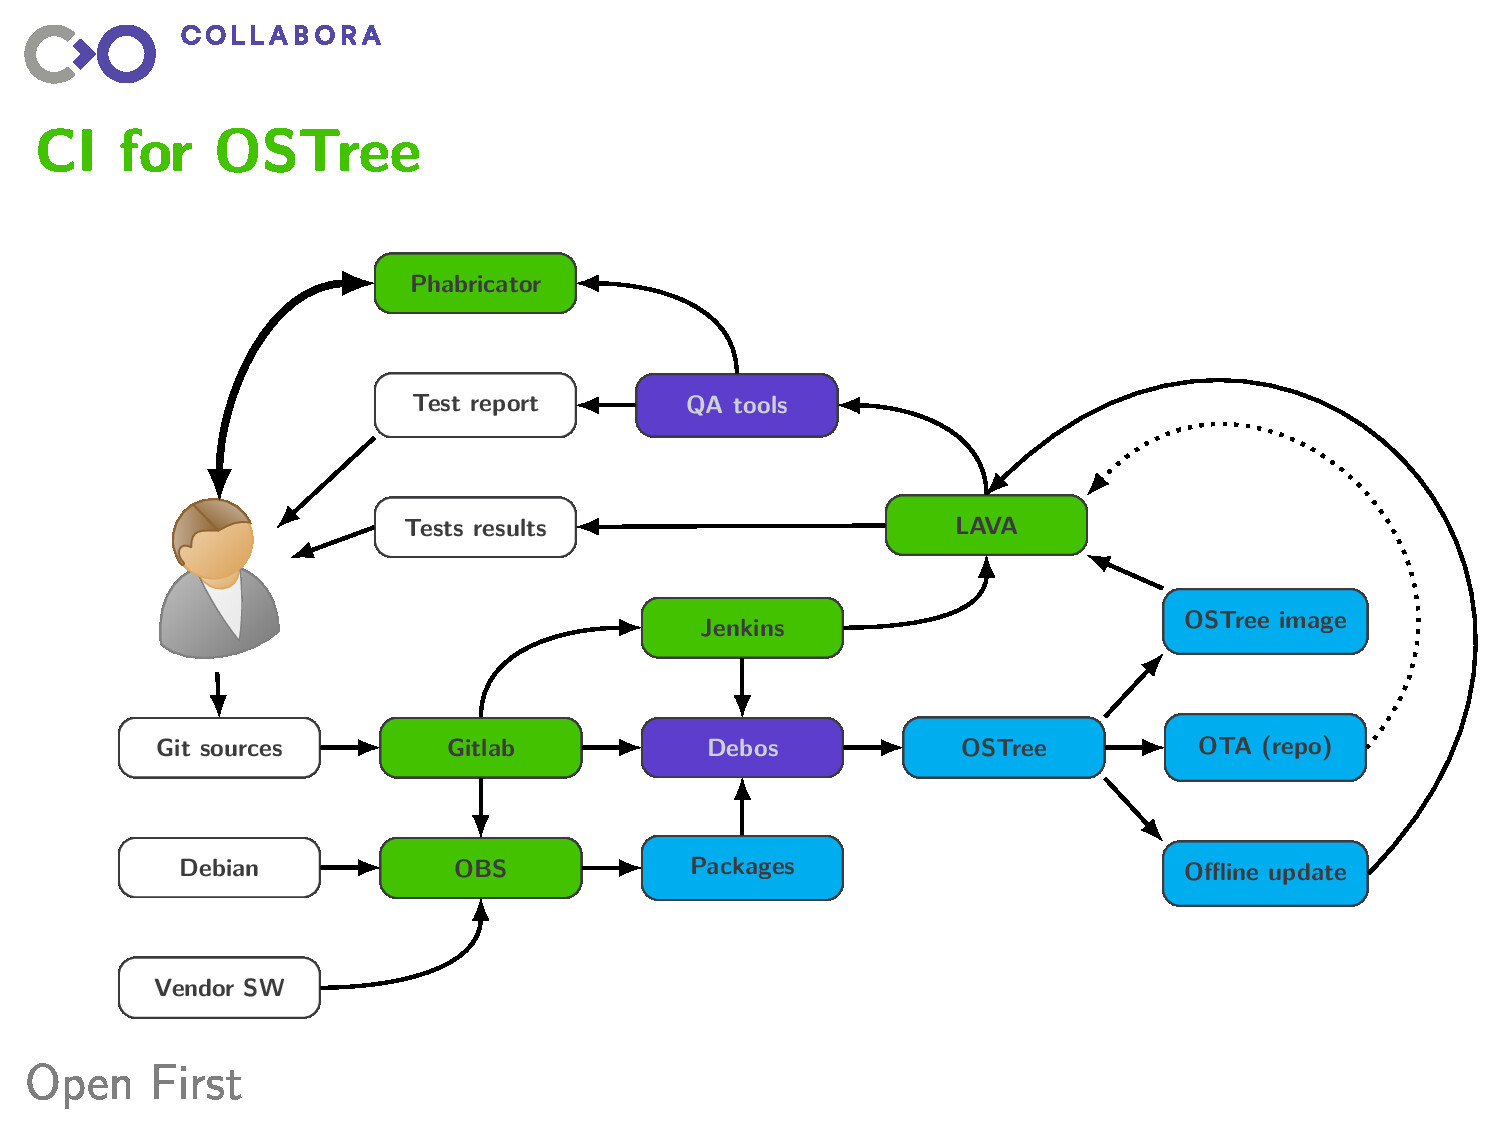
\includegraphics[width=10cm]{2019_Pynkin}  
  \label{pynkin:fig1}
\end{figure}
\end{center} 


Для обеспечения автоматической сборки и тестирования пакетов и готовых дисковых образов используются следующие системы и утилиты:

\begin{itemize}
  \item Gitlab\cite{bib10} --- хранение и ревью исходного кода;
  \item Phabricator\cite{bib11} --- управление проектом и трекер ошибок;
  \item Jenkins\cite{bib12} --- управление сборочными процессами;
  \item Open Build Service\cite{bib13} --- сборка и публикация пакетной базы;
  \item Debos\cite{bib7} --- утилита для создания загрузочных образов дисков;
  \item LAVA\cite{bib14} --- автоматическое тестирование собранных дисковых образов;
  \item QA Apertis\cite{bib15} --- тесты и набор скриптов для анализа результатов тестования, а также генерации отчетов.
\end{itemize}

В документации\cite{bib3} присутствует описание настройки ключевых компонентов для создания своей собственной инфраструктуры при необходимости.

\section*{Использованные источники}

\begin{thebibliography}{9}
\bibitem{bib1} \url{https://apertis.org}
\bibitem{bib2} \url{https://ostree.readthedocs.io}
\bibitem{bib3} \url{https://designs.apertis.org}
\bibitem{bib4} \url{https://wiki.apertis.org}
\bibitem{bib5} \url{https://gitlab.apertis.org/appfw/apertis-update-manager}
\bibitem{bib6} Пынькин Д.А., OSTree --- атомарные обновления ОС в стиле git, 2018, \url{https://lvee.org/ru/abstracts/289}
\bibitem{bib7} \url{https://github.com/go-debos/debos}
\bibitem{bib8} Пынькин Д.А., Debos --- еще одна утилита для создания ОС, 2018, \url{https://lvee.org/en/abstracts/263}
\bibitem{bib9} \url{https://github.com/go-debos/fakemachine}
\bibitem{bib9} \url{https://about.gitlab.com/}
\bibitem{bib10} \url{https://phacility.com/phabricator/}
\bibitem{bib11} \url{https://jenkins.io}
\bibitem{bib12} \url{https://openbuildservice.org/}
\bibitem{bib13} \url{https://www.lavasoftware.org/}
\bibitem{bib14} \url{https://qa.apertis.org/}
\bibitem{bib15} \url{https://gitlab.apertis.org/tests/apertis-test-cases}
\end{thebibliography}
\end{document}

\documentclass[10pt, a5paper]{article}
\usepackage{pdfpages}
\usepackage{parallel}
\usepackage[T2A]{fontenc}
\usepackage{ucs}
\usepackage[utf8x]{inputenc}
\usepackage[polish,english,russian]{babel}
\usepackage{hyperref}
\usepackage{rotating}
\usepackage[inner=2cm,top=1.8cm,outer=2cm,bottom=2.3cm,nohead]{geometry}
\usepackage{listings}
\usepackage{graphicx}
\usepackage{wrapfig}
\usepackage{longtable}
\usepackage{indentfirst}
\usepackage{array}
\newcolumntype{P}[1]{>{\raggedright\arraybackslash}p{#1}}
\frenchspacing
\usepackage{fixltx2e} %text sub- and superscripts
\usepackage{icomma} % коскі ў матэматычным рэжыме
\PreloadUnicodePage{4}

\newcommand{\longpage}{\enlargethispage{\baselineskip}}
\newcommand{\shortpage}{\enlargethispage{-\baselineskip}}

\def\switchlang#1{\expandafter\csname switchlang#1\endcsname}
\def\switchlangbe{
\let\saverefname=\refname%
\def\refname{Літаратура}%
\def\figurename{Іл.}%
}
\def\switchlangen{
\let\saverefname=\refname%
\def\refname{References}%
\def\figurename{Fig.}%
}
\def\switchlangru{
\let\saverefname=\refname%
\let\savefigurename=\figurename%
\def\refname{Литература}%
\def\figurename{Рис.}%
}

\hyphenation{admi-ni-stra-tive}
\hyphenation{ex-pe-ri-ence}
\hyphenation{fle-xi-bi-li-ty}
\hyphenation{Py-thon}
\hyphenation{ma-the-ma-ti-cal}
\hyphenation{re-ported}
\hyphenation{imp-le-menta-tions}
\hyphenation{pro-vides}
\hyphenation{en-gi-neering}
\hyphenation{com-pa-ti-bi-li-ty}
\hyphenation{im-pos-sible}
\hyphenation{desk-top}
\hyphenation{elec-tro-nic}
\hyphenation{com-pa-ny}
\hyphenation{de-ve-lop-ment}
\hyphenation{de-ve-loping}
\hyphenation{de-ve-lop}
\hyphenation{da-ta-ba-se}
\hyphenation{plat-forms}
\hyphenation{or-ga-ni-za-tion}
\hyphenation{pro-gramming}
\hyphenation{in-stru-ments}
\hyphenation{Li-nux}
\hyphenation{sour-ce}
\hyphenation{en-vi-ron-ment}
\hyphenation{Te-le-pathy}
\hyphenation{Li-nux-ov-ka}
\hyphenation{Open-BSD}
\hyphenation{Free-BSD}
\hyphenation{men-ti-on-ed}
\hyphenation{app-li-ca-tion}

\def\progref!#1!{\texttt{#1}}
\renewcommand{\arraystretch}{2} %Іначай формулы ў матрыцы зліпаюцца з лініямі
\usepackage{array}

\def\interview #1 (#2), #3, #4, #5\par{

\section[#1, #3, #4]{#1 -- #3, #4}
\def\qname{LVEE}
\def\aname{#1}
\def\q ##1\par{{\noindent \bf \qname: ##1 }\par}
\def\a{{\noindent \bf \aname: } \def\qname{L}\def\aname{#2}}
}

\def\interview* #1 (#2), #3, #4, #5\par{

\section*{#1\\{\small\rm #3, #4. #5}}

\def\qname{LVEE}
\def\aname{#1}
\def\q ##1\par{{\noindent \bf \qname: ##1 }\par}
\def\a{{\noindent \bf \aname: } \def\qname{L}\def\aname{#2}}
}

\switchlang{ru}
\begin{document}
\title{Сизиф на Эльбрусе: следующая станция}
\author{Михаил Шигорин, Москва, Россия\footnote{\url{mike@altlinux.org}, \url{http://lvee.org/ru/abstracts/314}}}
\maketitle
\begin{abstract}
Yes, we're rolling ALT p9 out with Elbrus support among the multitude of new primary and secondary platforms.
\end{abstract}
\section*{Девятая платформа}

Три года назад мой доклад был про выпуск восьмой платформы ALT; пришла пора и для девятой.  На этот раз мы делаем выпуск не только для 64/32-битных x86, но и для 64-битных ARM/Power в качестве основных платформ с обеспечением синхронной сборки в репозиторий, а также 64-битного RISC-V и 32-битных ARM/MIPSel в догоняющем режиме --- но для меня наиболее интересной новинкой является, конечно, доступность девятой платформы Альт на процессорах <<Эльбрус>> третьего и четвёртого поколения.
В сумме это всё даёт разработчикам и пользователям широчайшие возможности применения отечественных и перспективных мировых аппаратных архитектур при необходимости или желании отказаться от наследственной x86 со всем её грузом проблем (хотя стоит понимать, что такой груз разменивается на иной, а не исчезает).

\section*{Пакеты, версии, возможности}

Что нового по сравнению с прошлогодним выпуском, причисленным к восьмой платформе, но основанным на примерно среднем между p8 и p9 состоянии Сизифа, нашего репозитория разработки?

Разумеется, главное --- переход на новую ветку компилятора LCC: с 1.21 на 1.23.  Это дало базовую совместимость с GCC 5.5 вместо 4.8.0, в т.ч. поддержку C++11 (и частично C++14), а также несколько возросшую производительность собранного кода на том же оборудовании плюс возможность оптимизировать как под выбранное поколение, так и под конкретный процессор.

Обновлены и другие трансляторы, включая perl 5.28 с python 3.7; подтянут и сборочный инструментарий, в т.ч. meson 0.50 и cmake 3.11.  Также набор языков пополнился LISP (clisp, picolisp), R и базовым OCaml.  Разумеется, пополнились и обновились библиотеки, прикладные и серверные пакеты --- например, наконец-то осуществлён переход на единую Samba 4.10 вместо <<обычной>> и DC-сборок, Qt обновлена до 5.9, а список десктопных окружений пополнился Cinnamon 4.2.

Ну и тихо-незаметно обновили менеджер пакетов RPM до 4.13, а ядро Linux --- до 4.9 (над 4.19 в МЦСТ пока трудятся).

На \href{http://packages.altlinux.org}{packages.altlinux.org} добавлены сведения по наличию и версиям пакетов для e2k, а также их spec-файлы.

\section*{Формы распространения}

\noindent Наши наработки доступны теперь не только после установки обычных дистрибутивов <<Альт Сервер>> (\href{http://basealt.ru/products/alt-server}{basealt.ru/products/alt-server}) и <<Альт Рабочая станция>> (\href{http://basealt.ru/products/alt-workstation}{basealt.ru/products/alt-workstation}) в вариантах для Эльбруса, но и в добравшихся и сюда стартовых наборах.

К сожалению, работы поставщика по публикации набора разработчика под платформу Эльбрус (\url{http://mcst.ru/elbrus_pdk}) (PDK) пока не завершены и наши образы/репозитории тоже не могут быть выложены публично (доступны только покупателям соответствующего оборудования) --- но есть надежда на скорое улучшение этой ситуации.

Тем временем мы начали публикацию внутренних заметок и прочего полезного архитектурнозависимого знания в разделе вики \href{http://altlinux.org/elbrus}{altlinux.org/elbrus}.

\begin{center}
\begin{figure}[h!]
  \centering
  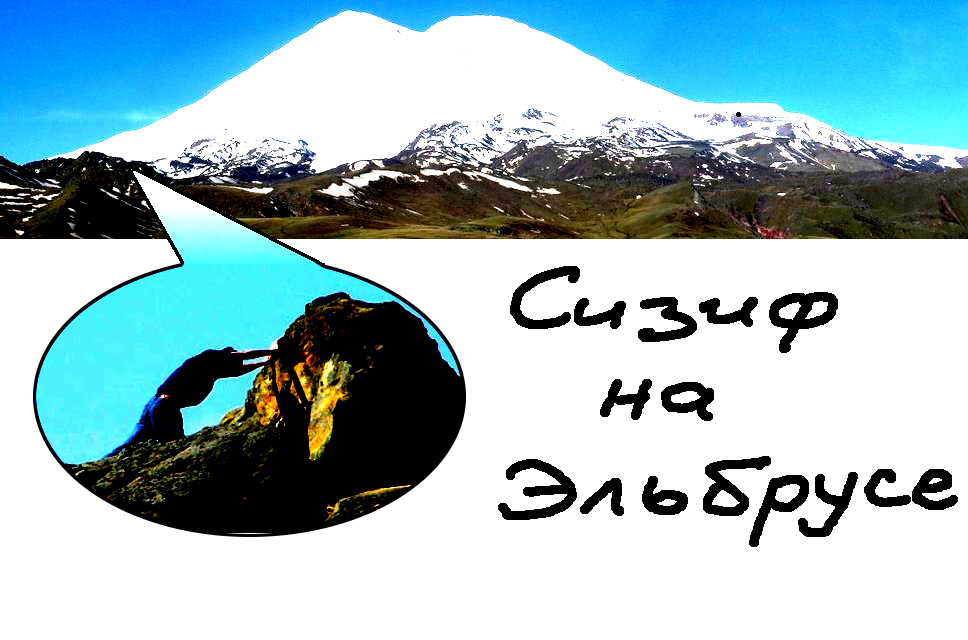
\includegraphics[width=10.8cm]{2019_Shigorin.png}

  \label{fig1}
\end{figure}
\end{center} 

\section*{Будни}

В общем, прорывов всё меньше, планомерной работы всё больше --- как и начинающих давать отдачу результатов её применения.
Кстати, я опять ищу помощников --- и спасибо LVEE за то, что Андрей Савченко уже откликнулся и вложил немало трудов в то, чтобы озвученное состоялось :)


\end{document}

\documentclass[10pt, a5paper]{article}
\usepackage{pdfpages}
\usepackage{parallel}
\usepackage[T2A]{fontenc}
\usepackage{ucs}
\usepackage[utf8x]{inputenc}
\usepackage[polish,english,russian]{babel}
\usepackage{hyperref}
\usepackage{rotating}
\usepackage[inner=2cm,top=1.8cm,outer=2cm,bottom=2.3cm,nohead]{geometry}
\usepackage{listings}
\usepackage{graphicx}
\usepackage{wrapfig}
\usepackage{longtable}
\usepackage{indentfirst}
\usepackage{array}
\newcolumntype{P}[1]{>{\raggedright\arraybackslash}p{#1}}
\frenchspacing
\usepackage{fixltx2e} %text sub- and superscripts
\usepackage{icomma} % коскі ў матэматычным рэжыме
\PreloadUnicodePage{4}

\newcommand{\longpage}{\enlargethispage{\baselineskip}}
\newcommand{\shortpage}{\enlargethispage{-\baselineskip}}

\def\switchlang#1{\expandafter\csname switchlang#1\endcsname}
\def\switchlangbe{
\let\saverefname=\refname%
\def\refname{Літаратура}%
\def\figurename{Іл.}%
}
\def\switchlangen{
\let\saverefname=\refname%
\def\refname{References}%
\def\figurename{Fig.}%
}
\def\switchlangru{
\let\saverefname=\refname%
\let\savefigurename=\figurename%
\def\refname{Литература}%
\def\figurename{Рис.}%
}

\hyphenation{admi-ni-stra-tive}
\hyphenation{ex-pe-ri-ence}
\hyphenation{fle-xi-bi-li-ty}
\hyphenation{Py-thon}
\hyphenation{ma-the-ma-ti-cal}
\hyphenation{re-ported}
\hyphenation{imp-le-menta-tions}
\hyphenation{pro-vides}
\hyphenation{en-gi-neering}
\hyphenation{com-pa-ti-bi-li-ty}
\hyphenation{im-pos-sible}
\hyphenation{desk-top}
\hyphenation{elec-tro-nic}
\hyphenation{com-pa-ny}
\hyphenation{de-ve-lop-ment}
\hyphenation{de-ve-loping}
\hyphenation{de-ve-lop}
\hyphenation{da-ta-ba-se}
\hyphenation{plat-forms}
\hyphenation{or-ga-ni-za-tion}
\hyphenation{pro-gramming}
\hyphenation{in-stru-ments}
\hyphenation{Li-nux}
\hyphenation{sour-ce}
\hyphenation{en-vi-ron-ment}
\hyphenation{Te-le-pathy}
\hyphenation{Li-nux-ov-ka}
\hyphenation{Open-BSD}
\hyphenation{Free-BSD}
\hyphenation{men-ti-on-ed}
\hyphenation{app-li-ca-tion}

\def\progref!#1!{\texttt{#1}}
\renewcommand{\arraystretch}{2} %Іначай формулы ў матрыцы зліпаюцца з лініямі
\usepackage{array}

\def\interview #1 (#2), #3, #4, #5\par{

\section[#1, #3, #4]{#1 -- #3, #4}
\def\qname{LVEE}
\def\aname{#1}
\def\q ##1\par{{\noindent \bf \qname: ##1 }\par}
\def\a{{\noindent \bf \aname: } \def\qname{L}\def\aname{#2}}
}

\def\interview* #1 (#2), #3, #4, #5\par{

\section*{#1\\{\small\rm #3, #4. #5}}

\def\qname{LVEE}
\def\aname{#1}
\def\q ##1\par{{\noindent \bf \qname: ##1 }\par}
\def\a{{\noindent \bf \aname: } \def\qname{L}\def\aname{#2}}
}

\switchlang{ru}
\begin{document}
\title{Dark Background and Light Text --- Firefox add-on}
\author{Mikhail Khvoinitsky, Минск, Belarus\footnote{\url{lvee.org@khvoinitsky.org}, \url{http://lvee.org/ru/abstracts/313}}}
\maketitle
\begin{abstract}
Modern Web is barely customizable. Most web designers try really hard to make their websites look the same for all users on all OSes and browsers and they try to eliminate any browser-specific behavior. This includes: font, font size, button placement guidelines (close button on the right or on the left, OK, Cancel buttons order and so on) and colors. We will concentrate on one problem: color customizability. People may want to override page colors for a variety of reasons: accessibility, preference to work in a dark room or just taste. But this is more complicated task rather than applying custom CSS with few overrides
\end{abstract}
Кастомизируемость современного веба оставляет желать лучшего. Большинство веб-дизайнеров стараются, чтобы их веб-сайты выглядели одинаково у всех пользователей независимо от их операционных систем, браузеров и, как следствие, их предпочтений. Но потребность в кастомизации есть. Например, не всегда стандартный размер шрифта подходит всем пользователям, да и сам шрифт не всегда выбирают как самый различимый. Также часто пользователи хотели бы видеть сайты в других цветах, часто в тёмных. Некоторые браузеры предоставляют возможность масштабирования страниц, а также игнорирования цветов, выставленных автором вебсайта, но часто это или слишком грубо (когда цвет текста несёт смысловую нагрузку, например, предупреждающая надпись на жёлтом фоне или программный код с подсвеченным синтаксисом), или этого недостаточно (есть ещё фоновые изображения). К счастью, уже все современные распространённые браузеры поддерживают расширения. Об одном таком, которое решает проблему изменения цветовой схемы страниц, и будет доклад, а также немного о смежных темах.

\subsection*{Краткое введение в то, что такое аддоны и что они могут делать}

Аудитория, думаю, прекрасно с этим понятием знакома и не раз пользовалась, но на всякий случай. Аддоны --- небольшие приложения на javascript для браузеров, которые могут незначительно встраиваться в UI браузеров (в виде кнопок, сайдбаров и хоткеев), а так же встраивать свой javascript и CSS в вебстраницы. Наиболее распространённый класс аддонов --- блокировщики рекламы.

\subsection*{Зачем люди могут предпочитать тёмные темы}

\begin{enumerate}
  \item Доступность. При некоторых патологиях зрения значительно проще воспринимать светлый текст на тёмном фоне.
  \item Удобство при работе в тёмной комнате (например, ночью). Поэтому часто такие темы называется ночным режимом (Night Mode).
  \item Личные вкусовые предпочтения.
\end{enumerate}

\subsection*{Ограничения user CSS как общего решения для изменения цветов сайтов}

\begin{enumerate}
  \item Узкоспециализированный CSS для конкретного вебсайта.\linebreak Плюсы: при желании и упорстве можно сделать очень качественно. Минусы: при малейшем изменении на сайте стиль поломается; требуется создавать подобный стиль вручную для каждого сайта.
  \item Грубо перекрасить \textbf{весь} текст и фон в нужные цвета. Плюсы: просто и быстро (как с точки зрения разработки, так и с точки зрения производительности). Минусы: потеряется вся цветовая семантика текста (например, подсветка синтаксиса кода, выделенное жёлтым предупреждение, красным ошибка и т. д.); фоновые изображения можно или все оставить, или все убрать (см. ниже о проблеме).
  \item CSS filter: invert и аналоги. Плюсы: просто с точки зрения разработки; для средней светлой страницы результат будет максимально качественным. Минусы: производительность ­— даже прокрутка страницы начнёт заметно подтормаживать (Firefox for Android становится практически неюзабельным); изначально тёмные страницы станут светлыми, смешанные страницы останутся смешанными, только наоборот.
\end{enumerate}

\subsection*{Решение на javascript, трудности с ним и их решения}

\begin{itemize}
  \item Обход и модификация стилей в <<document.styleSheets>>
  \item Изменение цвета на тёмный или светлый, сохранение тона (например, красный остаётся красным, но в зависимости от того, фон это или текст, становится тёмно-красным или светло-красным).
\begin{itemize}
  \item Преобразование цвета в пространство HSL, замена канала L (Lightness).
  \item Преобразование цвета в пространство YPbPr, замена канала Y.
\end{itemize}


  \item Фоновые изображения. Веб-стандарт никак не регламентирует указание того факта, несут ли фоновые изображения какую-либо смысловую нагрузку (например, это иконка на кнопке) или являются только декорацией (например, текстура на фоне текста). Решение: использование эвристики на основе различных параметров (URL, CSS-класс или id, значение background-repeat и т. д.).
\begin{itemize}
  \item Градиенты в качестве фоновых изображений. Решение: парсинг значений и обработка цветов как фоновых как в пункте выше.
\end{itemize}
\end{itemize}

\subsection*{Ссылки}

\begin{itemize}
  \item \href{https://addons.mozilla.org/firefox/addon/dark-background-light-text/}{addons.mozilla.org/firefox/addon/dark-background-light-text/}
  \item \href{https://github.com/m-khvoinitsky/dark-background-light-text-extension}{github.com/m-khvoinitsky/dark-background-light-text-extension}
\end{itemize}

\subsection*{Альтернативы, заслуживающие внимания}

\begin{itemize}
  \item \href{https://addons.mozilla.org/firefox/addon/darkreader/}{addons.mozilla.org/firefox/addon/darkreader/}
  \item \href{https://addons.mozilla.org/firefox/addon/midnight-lizard-quantum/}{addons.mozilla.org/firefox/addon/midnight-lizard-quantum/}
\end{itemize}

\subsection*{Краткая история технического устройство аддонов для Firefox}

\begin{itemize}
  \item overlay add-on\begin{itemize}
  \item Установка\textbackslash{}обновление только с перезагрузкой браузера
  \item Аддон имеет полный доступ к внутренним API браузера, никак не ограничен.
  \item Нет стабильного API --- аддоны могут спонтанно ломаться при обновлении браузера.
\end{itemize}


  \item bootstrapped add-on\begin{itemize}
  \item Первая попытка сделать аддоны безперезагрузочными
  \item Аддон начинается с файла bootstrap.js с функциями startup и shutdown, в которых разработчик должен сделать то, что хочет с браузером при помощи его DOM API.
  \item Все плюсы и минусы предыдущего типа, кроме необходимости перезагрузки браузера.
\end{itemize}


  \item Add-on SDK\begin{itemize}
  \item Попытка сделать стабильный API для аддонов.
  \item всё ещё есть возможность (теперь опциональная) получить доступ к внутренним API браузера (которое не имеет гарантии стабильности)
\end{itemize}


  \item WebExtensions\begin{itemize}
  \item Стабильное API и невозможность выйти за его пределы (последнее --- самый большой недостаток, который вызвал массу недовольств и даже сделал реализацию некоторых существующих аддонов невозможной)
  \item Причины появления:\begin{itemize}
  \item Необходимость закрыть внутренний API от аддонов, так как довольно сложно вносить изменения в браузер не ломая аддонов. Примеры крупных изменений, которые ломали аддоны: e10s (мультипроцессность), интеграция наработок из Servo.
  \item Трудности конкуренции с Chrome.
\end{itemize}


\end{itemize}


\end{itemize}

\end{document}

\documentclass[10pt, a5paper]{article}
\usepackage{pdfpages}
\usepackage{parallel}
\usepackage[T2A]{fontenc}
\usepackage{ucs}
\usepackage[utf8x]{inputenc}
\usepackage[polish,english,russian]{babel}
\usepackage{hyperref}
\usepackage{rotating}
\usepackage[inner=2cm,top=1.8cm,outer=2cm,bottom=2.3cm,nohead]{geometry}
\usepackage{listings}
\usepackage{graphicx}
\usepackage{wrapfig}
\usepackage{longtable}
\usepackage{indentfirst}
\usepackage{array}
\newcolumntype{P}[1]{>{\raggedright\arraybackslash}p{#1}}
\frenchspacing
\usepackage{fixltx2e} %text sub- and superscripts
\usepackage{icomma} % коскі ў матэматычным рэжыме
\PreloadUnicodePage{4}

\newcommand{\longpage}{\enlargethispage{\baselineskip}}
\newcommand{\shortpage}{\enlargethispage{-\baselineskip}}

\def\switchlang#1{\expandafter\csname switchlang#1\endcsname}
\def\switchlangbe{
\let\saverefname=\refname%
\def\refname{Літаратура}%
\def\figurename{Іл.}%
}
\def\switchlangen{
\let\saverefname=\refname%
\def\refname{References}%
\def\figurename{Fig.}%
}
\def\switchlangru{
\let\saverefname=\refname%
\let\savefigurename=\figurename%
\def\refname{Литература}%
\def\figurename{Рис.}%
}

\hyphenation{admi-ni-stra-tive}
\hyphenation{ex-pe-ri-ence}
\hyphenation{fle-xi-bi-li-ty}
\hyphenation{Py-thon}
\hyphenation{ma-the-ma-ti-cal}
\hyphenation{re-ported}
\hyphenation{imp-le-menta-tions}
\hyphenation{pro-vides}
\hyphenation{en-gi-neering}
\hyphenation{com-pa-ti-bi-li-ty}
\hyphenation{im-pos-sible}
\hyphenation{desk-top}
\hyphenation{elec-tro-nic}
\hyphenation{com-pa-ny}
\hyphenation{de-ve-lop-ment}
\hyphenation{de-ve-loping}
\hyphenation{de-ve-lop}
\hyphenation{da-ta-ba-se}
\hyphenation{plat-forms}
\hyphenation{or-ga-ni-za-tion}
\hyphenation{pro-gramming}
\hyphenation{in-stru-ments}
\hyphenation{Li-nux}
\hyphenation{sour-ce}
\hyphenation{en-vi-ron-ment}
\hyphenation{Te-le-pathy}
\hyphenation{Li-nux-ov-ka}
\hyphenation{Open-BSD}
\hyphenation{Free-BSD}
\hyphenation{men-ti-on-ed}
\hyphenation{app-li-ca-tion}

\def\progref!#1!{\texttt{#1}}
\renewcommand{\arraystretch}{2} %Іначай формулы ў матрыцы зліпаюцца з лініямі
\usepackage{array}

\def\interview #1 (#2), #3, #4, #5\par{

\section[#1, #3, #4]{#1 -- #3, #4}
\def\qname{LVEE}
\def\aname{#1}
\def\q ##1\par{{\noindent \bf \qname: ##1 }\par}
\def\a{{\noindent \bf \aname: } \def\qname{L}\def\aname{#2}}
}

\def\interview* #1 (#2), #3, #4, #5\par{

\section*{#1\\{\small\rm #3, #4. #5}}

\def\qname{LVEE}
\def\aname{#1}
\def\q ##1\par{{\noindent \bf \qname: ##1 }\par}
\def\a{{\noindent \bf \aname: } \def\qname{L}\def\aname{#2}}
}

\begin{document}
\title{Создание пакетов программной поддержки для процессоров собственной разработки}
\author{Роман Ставцев, Москва, Russian Federation\footnote{\url{lefty@mail.ru}, \url{http://lvee.org/ru/abstracts/302}}}
\maketitle
\begin{abstract}
The software development kit creating process for our own processors.
\end{abstract}
АО <<Байкал Электроникс>> фаблесс-компания специализируется на проектировании систем на кристалле (СнК) и интегральных микросхем. Основной продукцией является СнК \textbf{BE-T1000} и \textbf{BE-M1000}. Процессоры Baikal производятся на фабрике компании TSMC. Вспомогательной продукцией является программные пакеты (Software Development Kit, \textbf{SDK}) и оценочные платы.

Микропроцессор \textbf{BE-T1000}, другое название Байкал-Т1 относится к типу Система-на-кристале. Микропроцессор содержит два ядра MIPS32r5 P5600 Warrior.

\begin{center}
\begin{figure}[h!]
  \centering
  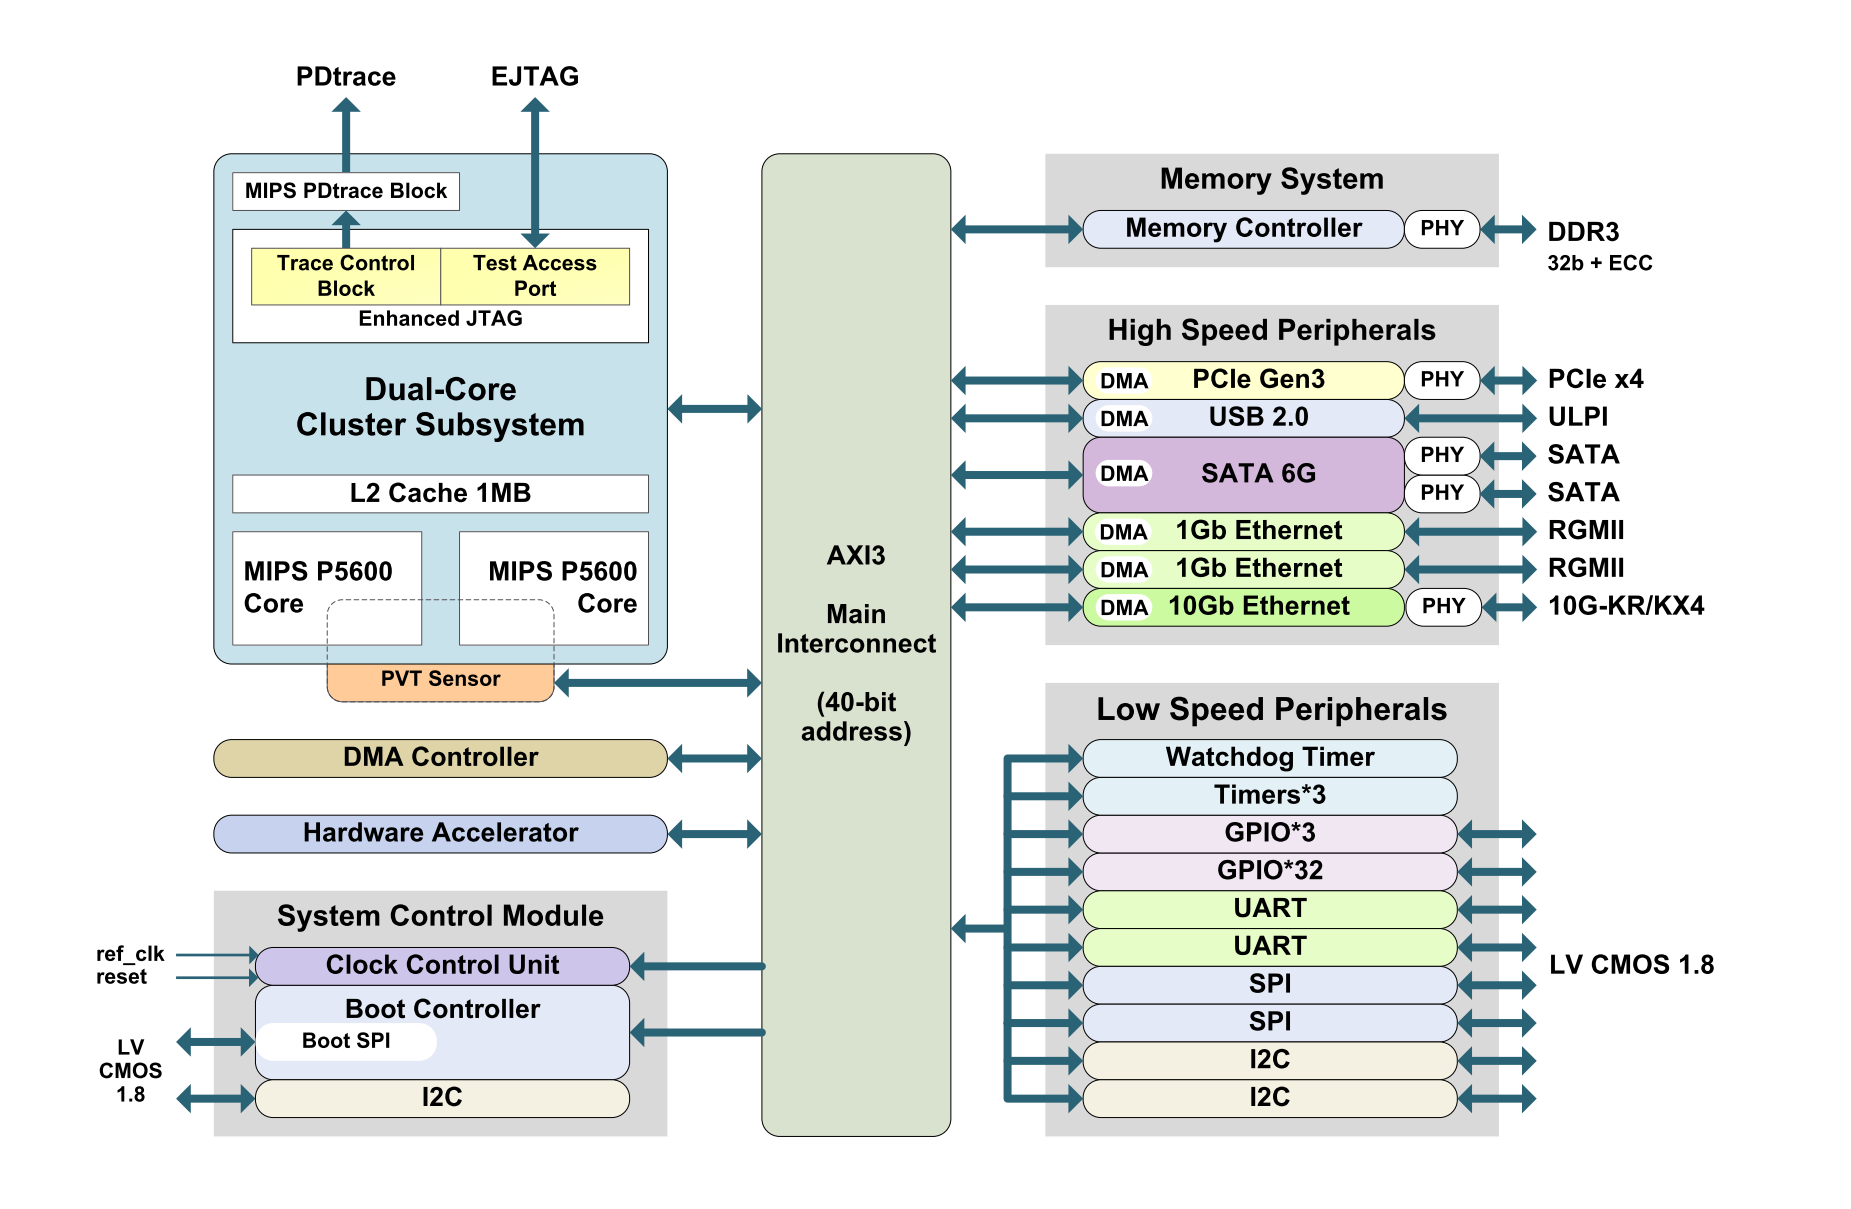
\includegraphics[width=10cm]{Stavtsev1}  
  \label{stavtsev:fig1}
\end{figure}
\end{center} 

Перечислим некоторые технические характеристики:

\begin{itemize}
  \item 2 ядра P5600 MIPS 32 r5, максимальная частота до 1,2 ГГц
  \item Кэш L2 1 Мбайт
  \item Контроллер памяти DDR3-1600
  \item Энергопотребление не более 5 Вт
*Технологический процесс 28 нм
\end{itemize}

Интегрированные интерфейсы:

\begin{itemize}
  \item 1 порт 10 Gb Ethernet
  \item 2 порта 1 Gb Ethernet
  \item контроллер PCIe Gen.3
  \item 2 порта SATA 3.0
  \item USB 2.0
\end{itemize}

Микропроцессор \textbf{BE---M1000}, другое название Байкал-M1 относится к типу Система-на-кристале.

\begin{center}
\begin{figure}[h!]
  \centering
  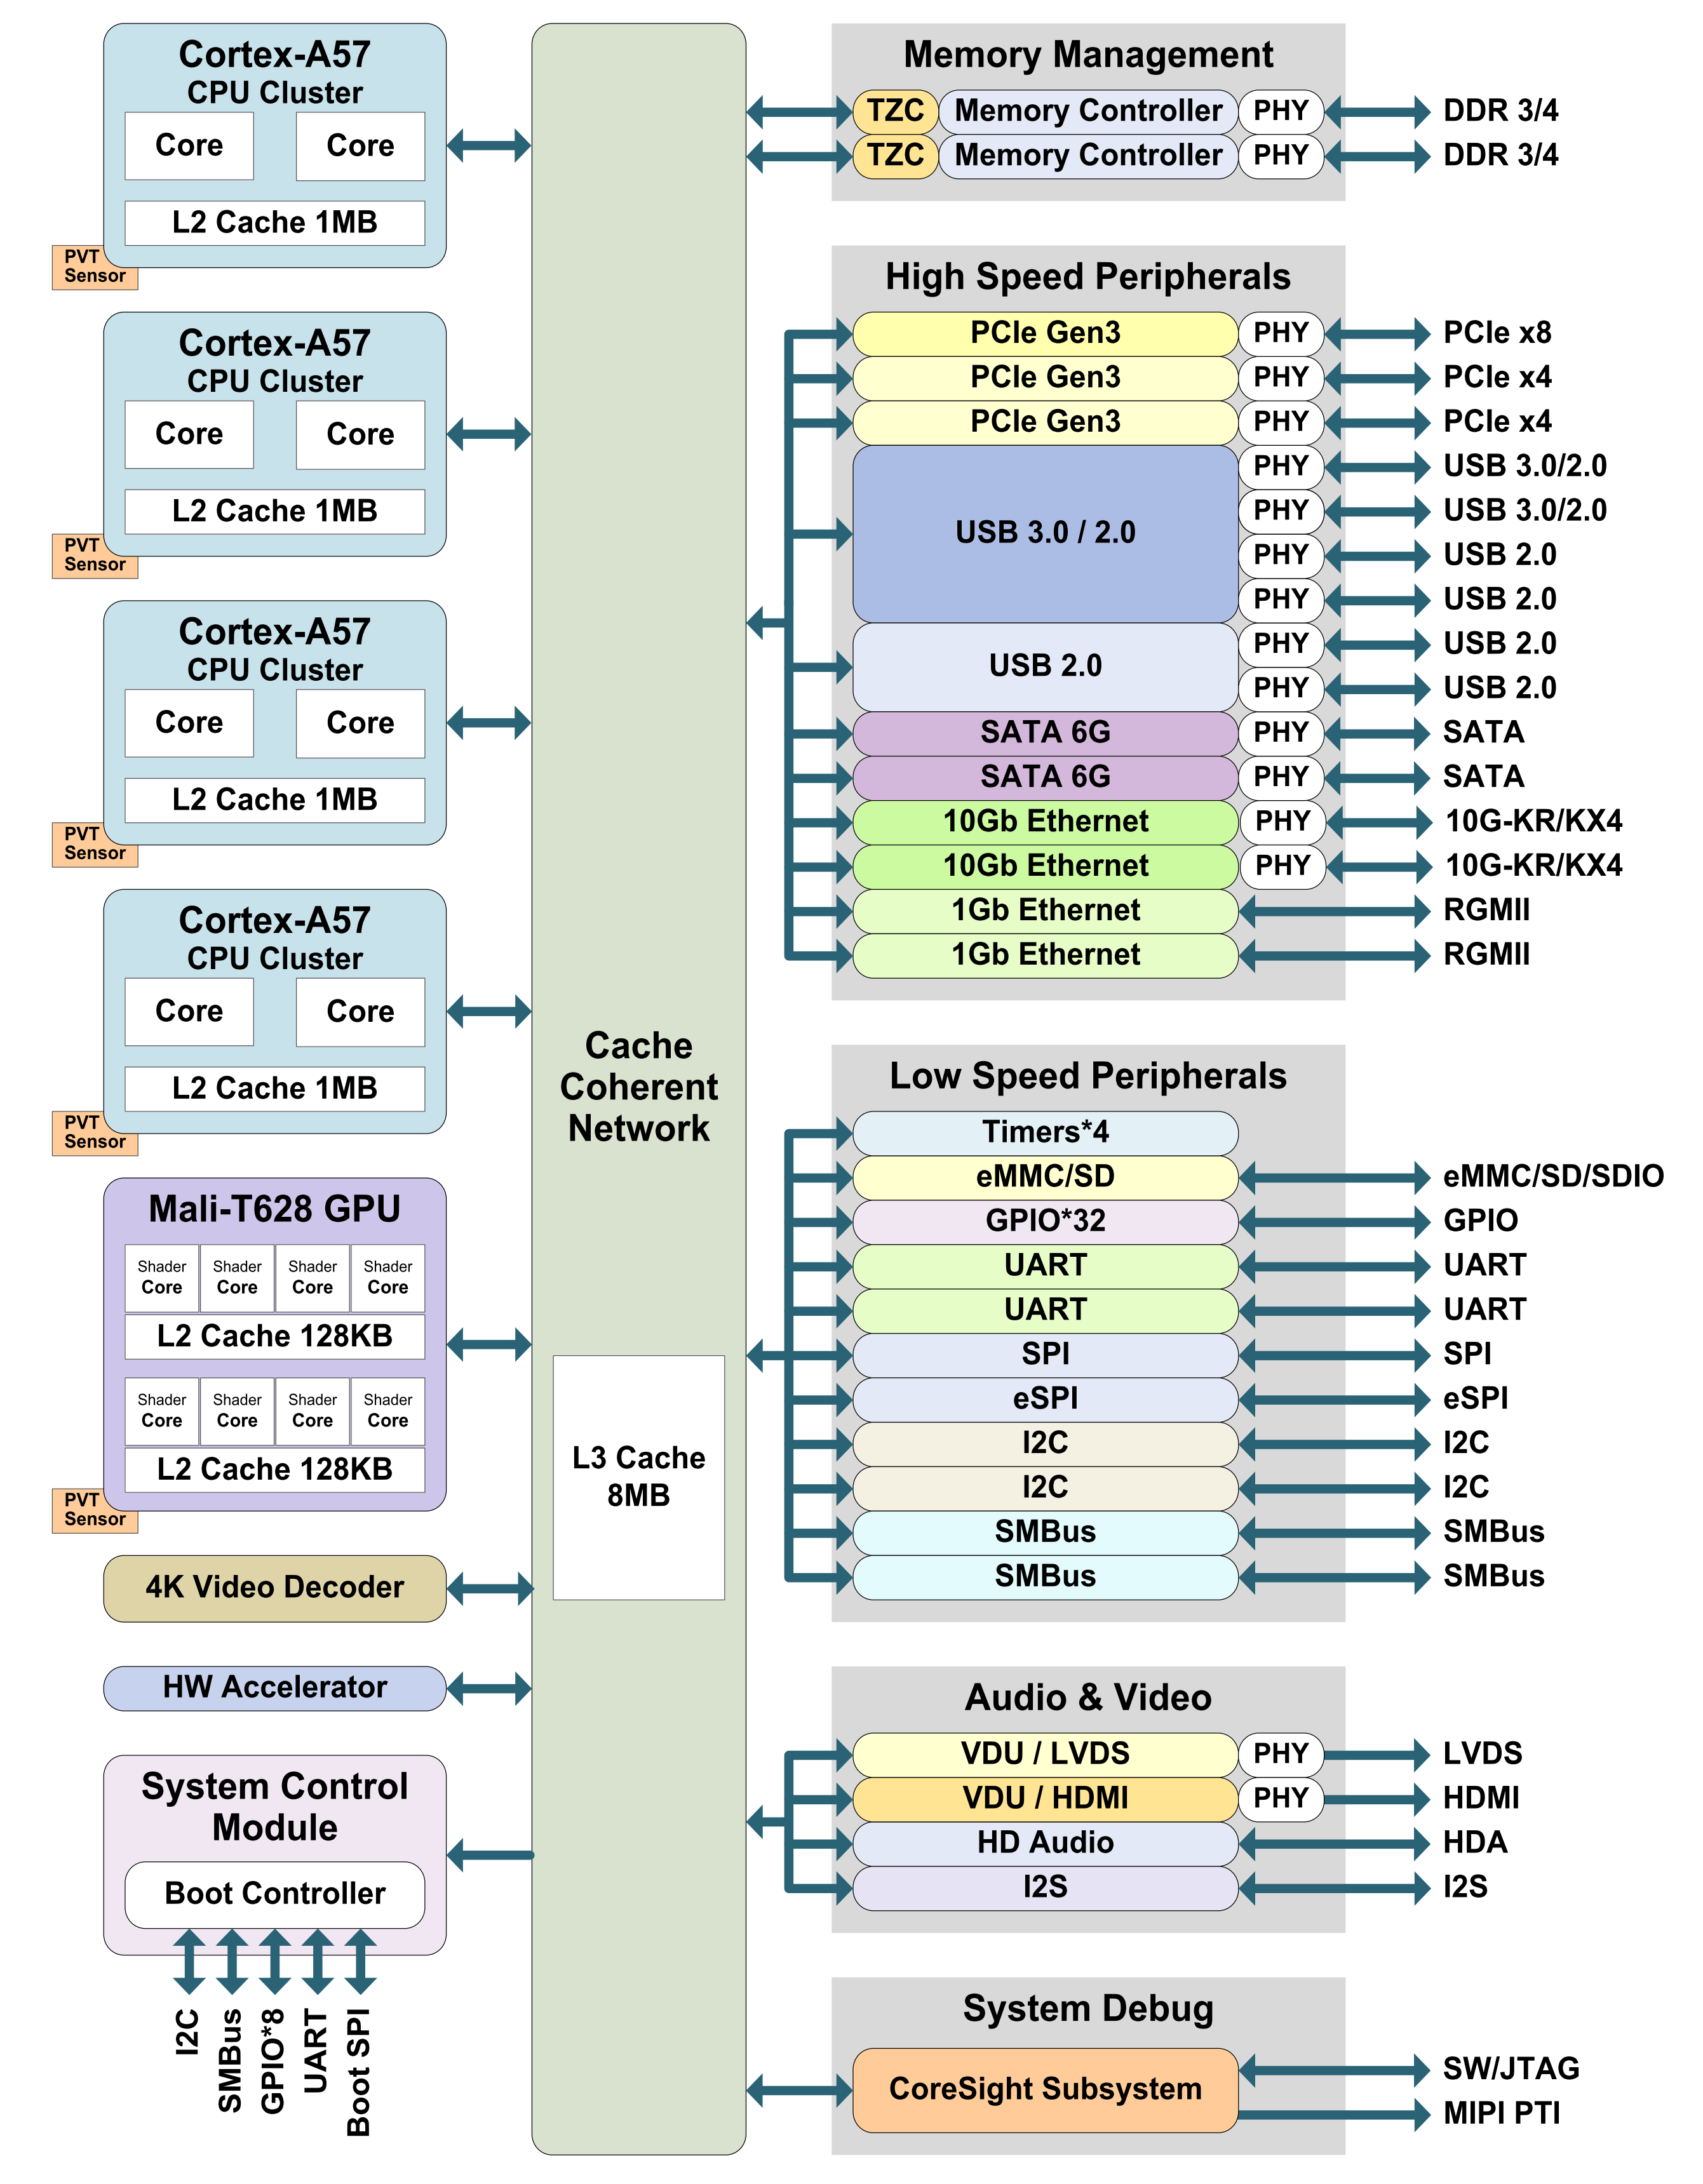
\includegraphics[width=10cm]{Stavtsev2}  
  \label{stavtsev:fig2}
\end{figure}
\end{center} 

Перечислим некоторые технические характеристики:

\begin{itemize}
  \item 4 кластера по 2 ядра ARM Cortex-A57, максимальная частота до 1,5ГГц
  \item Кэш L2 объемом 1 Мбайт на кластер
  \item Когерентный кэш L3 объемом 8 Мбайт
  \item 2 контроллера памяти DDR4-2400
  \item Графический процессор ARM Mail-T628 с поддержкой кэш L2 128 Кбайт на кластер
  \item 2 видеоконтроллера с поддержкой LVDS и HDMI2.0 интерфейсов
  \item Аппаратный 4K видео-декодер
  \item Аудио-подсистема HDAudio
  \item Подсистема управления загрузкой
  \item Технологический процесс 28 нм
  \item Корпус FCBGA 1521
\end{itemize}

Интегрированные интерфейсы:

\begin{itemize}
  \item 3 контроллера PCIe Gen3 (x8/x4/x4)
  \item 2 контроллера SATA 6G
  \item 2 контроллера XGb Ethernet
  \item 2 контроллера 1Gb Ethernet
  \item 2 контроллера USB 3.0/2.0 6 портов
\end{itemize}

Низкоскоростная периферия:

\begin{itemize}
  \item eMMC/SD/SDIO
  \item SPI/eSPI
  \item SMBus
  \item GPIO32
  \item UART
\end{itemize}

Программные пакеты \textbf{SDK} (Software Development Kit) для процессоров семейства Baikal, концентрируется на простоте установки и использования, предоставляя при этом необходимы инструментарий. В большей части SDK опирается на свободное программное обеспечение. Для каждого типа СнК выпускается свой SDK. SDK для BE-T1000 был основан на наборе собственных сборочных скриптов. Такой подход позволил создать автономную систему с минимумом зависимостей. Однако имеются и существенные ограничения в нашем решении, основное сложность создания изменяемых сборок с пользовательскими приложениями. При разработке SDK для BE-M1000 мы сохранили прежний принцип построения, понимая и принимая все плюсы и минусы такого решения.

Рассмотрим схожие компоненты SDK. В состав SDK входят средства разработки программ для целевого процессора, средства отладки, полный набор исходных кодов, комплект поддержки для отладочных/оценочных плат (BFK), образ встраиваемой операционной системы на основе ядра Linux и набора busybox, средства автоматизации сборки различных образов и прошивок для устройств на процессорах семейства Baikal.

Состав SDK выглядит следующим образом:

\begin{itemize}
  \item Загрузчик
  \item Ядро Linux
  \item Образ initrd встраиваемой ОС на основе пакета busybox
  \item Образ initramfs для запуска <<больших>> дистрибутивов ОС Linux
  \item Прошивка для загрузочной флеш-памяти
  \item Образ файловой системы для эмулятора QEMU
  \item Скрипты автоматизации сборки
  \item Тулчейн
  \item Вспомогательные утилиты
  \item Программный эмулятор
  \item Скрипты поддержки/автоматизации для эмулятора
  \item Исходные коды
\end{itemize}

Основные компоненты немного подробнее.

\subsection*{Загрузчик}

Мы используем модифицированную версию загрузчика U-BOOT для BE-T1000.
Начинали с U-BOOT v2014.10
Мы используем для BE-M1000 UEFI tianocore основанный на <<UEFI Development Kit>> UDK2017.

\subsection*{Ядро Linux}

для BE-T1000 были внесены дополнения в следующие ветки ядра Linux:
\begin{itemize}
\item 3.19.xx --- не поддерживается
\item 4.4.xx --- активно поддерживается (https://github.com/baikalelectronics/Linux-kernel.4.4.xx)
\item 5.2 --- в разработке
\end{itemize}
для BE-M1000 были внесены дополнения в следующие ветки ядра Linux
\begin{itemize}
\item 4.9.180 --- в разработке
\end{itemize}

\subsection*{Тулчейн}

Пакет средств кросс-компиляции на основе GNU gcc, binutils и т.д.
\begin{itemize}
\item gcc–8.3.0, binutils–2.32 (для BE-T1000, SDK-4.18)
\item gcc 6.3.0, binutils 2.28 (для BE-M1000)
\end{itemize}
Средства отладки (gdb)
\begin{itemize}
\item gdb–8.2.1 (для BE-T1000, SDK-4.18)
\item gdb 7.12.1 (для BE-M1000)
\end{itemize}
Предсобранные исполнимые файлы и библиотеки (sysroot) на основе glibc
\begin{itemize}
\item glibc–2.29 (для BE-T1000, SDK-4.18)
\item glibc 2.25 (для BE-M1000)
\end{itemize}

\end{document}

\documentclass[10pt, a5paper]{article}
\usepackage{pdfpages}
\usepackage{parallel}
\usepackage[T2A]{fontenc}
\usepackage{ucs}
\usepackage[utf8x]{inputenc}
\usepackage[polish,english,russian]{babel}
\usepackage{hyperref}
\usepackage{rotating}
\usepackage[inner=2cm,top=1.8cm,outer=2cm,bottom=2.3cm,nohead]{geometry}
\usepackage{listings}
\usepackage{graphicx}
\usepackage{wrapfig}
\usepackage{longtable}
\usepackage{indentfirst}
\usepackage{array}
\newcolumntype{P}[1]{>{\raggedright\arraybackslash}p{#1}}
\frenchspacing
\usepackage{fixltx2e} %text sub- and superscripts
\usepackage{icomma} % коскі ў матэматычным рэжыме
\PreloadUnicodePage{4}

\newcommand{\longpage}{\enlargethispage{\baselineskip}}
\newcommand{\shortpage}{\enlargethispage{-\baselineskip}}

\def\switchlang#1{\expandafter\csname switchlang#1\endcsname}
\def\switchlangbe{
\let\saverefname=\refname%
\def\refname{Літаратура}%
\def\figurename{Іл.}%
}
\def\switchlangen{
\let\saverefname=\refname%
\def\refname{References}%
\def\figurename{Fig.}%
}
\def\switchlangru{
\let\saverefname=\refname%
\let\savefigurename=\figurename%
\def\refname{Литература}%
\def\figurename{Рис.}%
}

\hyphenation{admi-ni-stra-tive}
\hyphenation{ex-pe-ri-ence}
\hyphenation{fle-xi-bi-li-ty}
\hyphenation{Py-thon}
\hyphenation{ma-the-ma-ti-cal}
\hyphenation{re-ported}
\hyphenation{imp-le-menta-tions}
\hyphenation{pro-vides}
\hyphenation{en-gi-neering}
\hyphenation{com-pa-ti-bi-li-ty}
\hyphenation{im-pos-sible}
\hyphenation{desk-top}
\hyphenation{elec-tro-nic}
\hyphenation{com-pa-ny}
\hyphenation{de-ve-lop-ment}
\hyphenation{de-ve-loping}
\hyphenation{de-ve-lop}
\hyphenation{da-ta-ba-se}
\hyphenation{plat-forms}
\hyphenation{or-ga-ni-za-tion}
\hyphenation{pro-gramming}
\hyphenation{in-stru-ments}
\hyphenation{Li-nux}
\hyphenation{sour-ce}
\hyphenation{en-vi-ron-ment}
\hyphenation{Te-le-pathy}
\hyphenation{Li-nux-ov-ka}
\hyphenation{Open-BSD}
\hyphenation{Free-BSD}
\hyphenation{men-ti-on-ed}
\hyphenation{app-li-ca-tion}

\def\progref!#1!{\texttt{#1}}
\renewcommand{\arraystretch}{2} %Іначай формулы ў матрыцы зліпаюцца з лініямі
\usepackage{array}

\def\interview #1 (#2), #3, #4, #5\par{

\section[#1, #3, #4]{#1 -- #3, #4}
\def\qname{LVEE}
\def\aname{#1}
\def\q ##1\par{{\noindent \bf \qname: ##1 }\par}
\def\a{{\noindent \bf \aname: } \def\qname{L}\def\aname{#2}}
}

\def\interview* #1 (#2), #3, #4, #5\par{

\section*{#1\\{\small\rm #3, #4. #5}}

\def\qname{LVEE}
\def\aname{#1}
\def\q ##1\par{{\noindent \bf \qname: ##1 }\par}
\def\a{{\noindent \bf \aname: } \def\qname{L}\def\aname{#2}}
}

\switchlang{en}
\begin{document}
\title{Speed-up Solving Linear Systems on Parallel Architectures via Aggregation of Clans}
\author{Dmitry Zaitsev, Odessa, Ukraine\footnote{\url{daze@acm.org}, \url {https://lvee.org/ru/abstracts/298}}}
\maketitle
\begin{abstract}
Varying minimal clan size brings in certain imbalance when solving a linear (Diophantine) system on parallel architectures via composition of its clans using open source software PaAd. The problem is partially mended by dynamic scheduling of jobs. The present paper studies a task of preliminary balancing the clan size via their aggregation represented as a special case of graph partitioning. Due to complexity of the optimization criteria, taking into consideration both the number of equations and the number of variables on two stages of solution -- solving a system for each clan and solving a composition system -- simplified variants of the task are considered and solved using heuristic techniques: a fast bin packing with the first fit on a sorted array algorithm and a multi-objective graph partitioning with software package METIS. Obtained benchmarks show that aggregation of clans brings in an additional 3 times speed-up.
\end{abstract}
\subsection*{Introduction}

The technique for the composition of linear system clans \cite{bib1} has been further developed with regard to modern parallel architectures and applied to speed-up solving systems of linear Diophantine equations \cite{bib2}, open source software package ParAd released \cite{bib3}.

Solving linear systems is a central task of numerical methods. That is why LAPACK \cite{bib4} is one of the most widespread packets in the world which is applied for benchmarks, including modern supercomputers domain.

Diophantine systems are defined over integer numbers and they appear in manifold application areas, for instance in model-checking with Petri nets for verification of networking protocols \cite{bib5}, manufacture control, data encryption, and artificial intelligence \cite{bib6}. Since the \linebreak computational complexity of solving Diophantine systems is higher than for systems over real numbers, methods to speed-up the process are in demand.

It is convenient to represent (sparse) linear systems as Petri net graphs, equations correspond to transitions (rectangles), variables \linebreak correspond to places (circles). A clan is a subset of the system equations \cite{bib1}. In the decomposition graph \cite{bib1}, each vertex corresponds to a clan; vertices are connected in case the corresponding equations contain common variables.

In the present paper, we specify the clan aggregation task as a special case of graph partitioning \cite{bib7} for a weighted graph having two weights of a node and one weight of an edge. The node weights \linebreak correspond to the number of equations and the number of internal variables of a clan while the edge weight corresponds to the number of contact variables connecting a pair of clans. The optimization criterion should take into consideration the complexity of solving systems for clans and solving the composition system.

Here, for hypertorus 4D of size 3 communication structure, 2D example of size 2 follows

\begin{center}
\begin{figure}[h!]
  \centering
  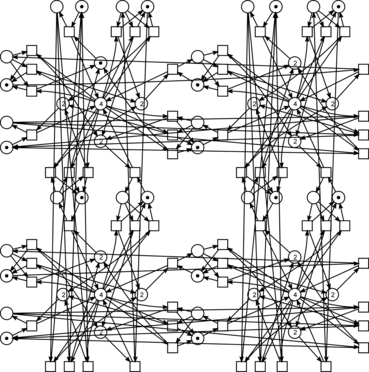
\includegraphics[width=8cm]{Zaitsev1.png}

  \label{fig1}
\end{figure}
\end{center}

\noindent we compare the decomposition graph

\begin{center}
\begin{figure}[h!]
  \centering
  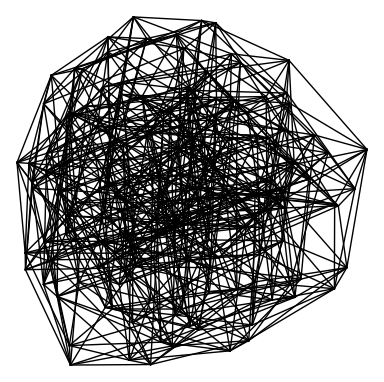
\includegraphics[width=8cm]{Zaitsev2.png}

  \label{fig1}
\end{figure}
\end{center}

\noindent and its aggregation into 7 clans (on the number of available processors minus one)

\begin{center}
\begin{figure}[h!]
  \centering
  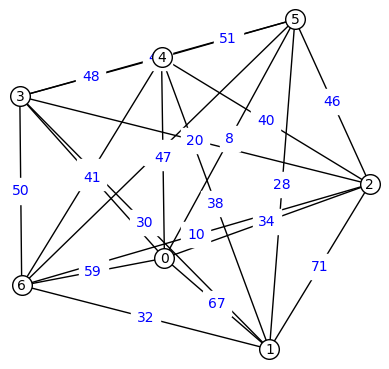
\includegraphics[width=8cm]{Zaitsev3.png}

  \label{fig1}
\end{figure}
\end{center}

A new version of ParAd is released \cite{bib3}, benchmarks for clans \linebreak aggregation are obtained on series of sparse integer matrices which represent Petri net models from Model Checking Contest and \linebreak acknowledged by some tests for real matrices from MatrixMarket and SuiteSparse collections. Aggregation brings-in an additional 3 times speed-up. The speed-up is obtained due to the static load balancing for distributed computing nodes.

\subsection*{Aggregation vs Composition}

We represent the source decomposition of a given system (matrix) into its minimal clans by a weighted graph of the first kind. We use the first kind decomposition graph to aggregate clans for the load balancing. Since at the first stage, a system is solved for each clan, our local goal is to have all the clans merely of the same size. In an ideal case, we need to minimize the number of basis solution as well and this goal is achieved when having merely the same number of equations and variables.

Granulation of the clan technique is limited by the maximal clan size. Thus this value restricts other parameters of the clan aggregation. In other words, when aggregating a subset of clans, the number of equations is summed up while contact variables within sub-graph become internal variables of the aggregated clan, internal variables are summed up as well.

Suppose an aggregated decomposition graph of the first kind is obtained. The first stage of the composition solution of a system is solving a system of equations for each clan. After solving these systems, a decomposition graph of the second kind is obtained. It coincides with the decomposition graph of the first kind with except weights of vertices.

The second kind decomposition graph is employed for either \linebreak simultaneous or sequential or parallel-sequential composition of clans. When a composition system is created, the number of basis solutions (the vertex weights) corresponds to the number of variables while the number of contact variables (the edge weights) corresponds to the number of equations.

The same as for aggregation, the composition operation is \linebreak represented by the sub-graph contraction. Though our goal is to contract a graph into a single vertex finally while for aggregation our goal is to achieve the best edge-cut and the vertex weight balance. That is why the process of composition is called a graph collapse. Recalculation of the vertex weights is reasonable for (parallel-) sequential composition only; for simultaneous composition, it only indicates the number of finally obtained basis solutions.

Thus, after aggregation of clans, the composition process looks the same as described in early works with the only difference we started taking into consideration the vertex weight. In the present paper, we consider global criteria of optimization with regard to the simultaneous composition of clans only. Sequential and parallel-sequential \linebreak composition of clans produce a rather sophisticated sequence of changes for vertex weights and here we do not develop further results on the quasi-optimal collapse of the weighted graph obtained in (for graphs with the edge weights only).

We study the task of clans aggregations separately through global optimization criteria should be considered to choose the proper criterion for aggregation. The global goal consists in minimization of the total time of solving a given system which includes the following stages: decomposition, aggregation, solving systems for clans, composition, \linebreak basis matrix multiplication. In this consideration, we suppose the \linebreak simultaneous composition of clans and the main criterion of \linebreak minimization is the composition system size. For a series of studied systems, exactly a comparably big composition system constituted a bottleneck for the entire process.

\subsection*{Aggregation of Clans via Graph Partitioning using METIS}

A well-known task of k-way graph partitioning is very close to the clan aggregation objectives and METIS \cite{bib7} is one of the best software packages for graph partitioning and it is open source software under Apache 2.0 license. METIS partitions a graph into k parts using either the multilevel recursive bisection or the multilevel k-way partitioning paradigms and achieves rather good performance. It accepts a scalar weight of an edge and a vector of weights for a vertex. The primary METIS objective is the minimization of the edge-cut --- the sum of edge weights of the obtained graph. Besides, it takes into consideration multiple balancing constraints, for instance, the vertex weights equally distributed among the obtained parts.

Thus the primary objective --- the minimal size of composition system --- is completely achieved by METIS while the secondary \linebreak objective of having merely the same size of the clans' systems is achieved partially. Since we can not express transformations of the second vertex weight, we omit it in the decomposition graph specification.

After the decomposition into minimal clans, we compute the number of parts the decomposition graph is partitioned into, and transform the ParAd data structures into METIS API form which is based on the row-compressed representation of a sparse matrix to define the graph adjacency relation and vectors of weights. As a result, METIS produces a vector assigning the partition number to each vertex. According to this vector, the clan decomposition data --- decomposition graph, clans and contact variables specifications --- are reorganized. The rest of ParAd code \cite{bib3} is unchanged: it goes on aggregated clans in the same way as on minimal clans.

\subsection*{Benchmarks for Clans Aggregation}

The following benchmarks have been obtained on cluster Saturn and computer Hare \cite{bib2}. We obtain basic benchmarks solving homogeneous Diophantine systems for Petri net models collection. The following models are considered:

\begin{itemize}
  \item al --- a simplified version of a landing detector for an airplane;
  \item af --- an automatic flight control system;
  \item cd --- a cloud application deployment;
  \item dc --- a distributed language compiler;
  \item ht --- hypertorus communication grid;
  \item sm --- processes sharing memory.
\end{itemize}

The optimum is achieved somewhere in the middle with the number of aggregated clans that provides the merely equal size of the system on two stages of the compositional solution. The two-letter names are used as prefixes in the names of ParAd tests \cite{bib3} and in the following graph where data is measured in the times of speed-ups comparing the ParAd version without aggregation:

\begin{center}
\begin{figure}[h!]
  \centering
  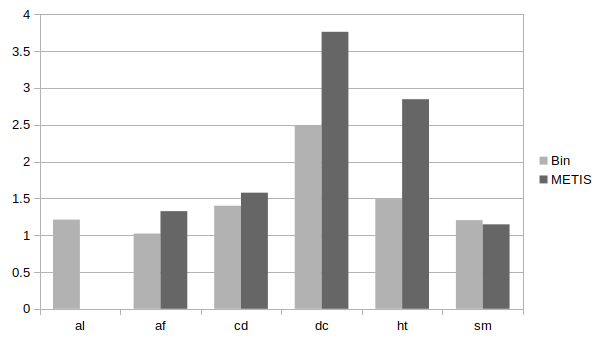
\includegraphics[width=8cm]{Zaitsev4.png}

  \label{fig1}
\end{figure}
\end{center}

METIS \cite{bib7} gives rather good results allowing us to speed-up \linebreak computations a few times, the maximal speed-up of 4 times has been obtained for hypertorus with the higher number of dimensions.

\subsection*{Conclusions}

A series of benchmarks has been obtained for Petri net models and collections of sparse matrices which acknowledge benefits of the developed clan aggregation modules included into a new release of ParAd package \cite{bib3}. Considerable speed-up of 3 times has been obtained solving both Diophantine systems and systems over real numbers.

\subsection*{References}

\begin{thebibliography}{9}
\bibitem{bib1} {Zaitsev D.A. Sequential composition of linear systems’ clans, Information Sciences, Vol. 363, 292–307. http://dx.doi.org/10.1016/j.ins.2016.02.016}
\bibitem{bib2} {Dmitry Zaitsev, Stanimire Tomov, Jack Dongarra. Solving Linear Diophantine Systems on Parallel Architectures, IEEE Transactions on Parallel and Distributed Systems, 30(5), 2019, 1158–1169. http://dx.doi.org/10.1109/TPDS.2018.2873354}
\bibitem{bib3} {ParAd: Solve a linear Diophantine homogeneous (sparse) system via composition of its clans on parallel architectures, https://github.com/dazeorgacm/ParAd}
\bibitem{bib4} {LAPACK — Linear Algebra PACKage, http://www.netlib.org/lapack}
\bibitem{bib5} {Zaitsev D.A. Clans of Petri Nets: Verification of protocols and performance evaluation of networks, LAP LAMBERT Academic Publishing, 2013, 292 p. http://daze.ho.ua/daze-clans-covered-draft.djvu}
\bibitem{bib6} {Zaitsev D.A. Sleptsov Nets Run Fast, IEEE Transactions on Systems, Man, and Cybernetics: Systems, 2016, Vol. 46, No. 5, 682 -- 693. http://dx.doi.org/10.1109/TSMC.2015.2444414}
\bibitem{bib7} {George Karypis. 2019. METIS -- Serial Graph Partitioning and Fill-reducing Matrix Ordering. http://glaros.dtc.umn.edu/gkhome/metis/metis/overview}\end{thebibliography}
\end{document}

\documentclass[10pt, a5paper]{article}
\usepackage{pdfpages}
\usepackage{parallel}
\usepackage[T2A]{fontenc}
\usepackage{ucs}
\usepackage[utf8x]{inputenc}
\usepackage[polish,english,russian]{babel}
\usepackage{hyperref}
\usepackage{rotating}
\usepackage[inner=2cm,top=1.8cm,outer=2cm,bottom=2.3cm,nohead]{geometry}
\usepackage{listings}
\usepackage{graphicx}
\usepackage{wrapfig}
\usepackage{longtable}
\usepackage{indentfirst}
\usepackage{array}
\newcolumntype{P}[1]{>{\raggedright\arraybackslash}p{#1}}
\frenchspacing
\usepackage{fixltx2e} %text sub- and superscripts
\usepackage{icomma} % коскі ў матэматычным рэжыме
\PreloadUnicodePage{4}

\newcommand{\longpage}{\enlargethispage{\baselineskip}}
\newcommand{\shortpage}{\enlargethispage{-\baselineskip}}

\def\switchlang#1{\expandafter\csname switchlang#1\endcsname}
\def\switchlangbe{
\let\saverefname=\refname%
\def\refname{Літаратура}%
\def\figurename{Іл.}%
}
\def\switchlangen{
\let\saverefname=\refname%
\def\refname{References}%
\def\figurename{Fig.}%
}
\def\switchlangru{
\let\saverefname=\refname%
\let\savefigurename=\figurename%
\def\refname{Литература}%
\def\figurename{Рис.}%
}

\hyphenation{admi-ni-stra-tive}
\hyphenation{ex-pe-ri-ence}
\hyphenation{fle-xi-bi-li-ty}
\hyphenation{Py-thon}
\hyphenation{ma-the-ma-ti-cal}
\hyphenation{re-ported}
\hyphenation{imp-le-menta-tions}
\hyphenation{pro-vides}
\hyphenation{en-gi-neering}
\hyphenation{com-pa-ti-bi-li-ty}
\hyphenation{im-pos-sible}
\hyphenation{desk-top}
\hyphenation{elec-tro-nic}
\hyphenation{com-pa-ny}
\hyphenation{de-ve-lop-ment}
\hyphenation{de-ve-loping}
\hyphenation{de-ve-lop}
\hyphenation{da-ta-ba-se}
\hyphenation{plat-forms}
\hyphenation{or-ga-ni-za-tion}
\hyphenation{pro-gramming}
\hyphenation{in-stru-ments}
\hyphenation{Li-nux}
\hyphenation{sour-ce}
\hyphenation{en-vi-ron-ment}
\hyphenation{Te-le-pathy}
\hyphenation{Li-nux-ov-ka}
\hyphenation{Open-BSD}
\hyphenation{Free-BSD}
\hyphenation{men-ti-on-ed}
\hyphenation{app-li-ca-tion}

\def\progref!#1!{\texttt{#1}}
\renewcommand{\arraystretch}{2} %Іначай формулы ў матрыцы зліпаюцца з лініямі
\usepackage{array}

\def\interview #1 (#2), #3, #4, #5\par{

\section[#1, #3, #4]{#1 -- #3, #4}
\def\qname{LVEE}
\def\aname{#1}
\def\q ##1\par{{\noindent \bf \qname: ##1 }\par}
\def\a{{\noindent \bf \aname: } \def\qname{L}\def\aname{#2}}
}

\def\interview* #1 (#2), #3, #4, #5\par{

\section*{#1\\{\small\rm #3, #4. #5}}

\def\qname{LVEE}
\def\aname{#1}
\def\q ##1\par{{\noindent \bf \qname: ##1 }\par}
\def\a{{\noindent \bf \aname: } \def\qname{L}\def\aname{#2}}
}

\switchlang{en}
\begin{document}
\title{Software Generators of Petri Net Models}
\author{Tatiana R. Shmeleva, Odessa, Ukraine\footnote{\url{tishtri@rambler.ru}, \url {https://lvee.org/ru/abstracts/299}}}
\maketitle
\begin{abstract}
Petri net models of variable size having definite structure are characteristic for manifold application domains such as \linebreak networking and high performance computing, manufacturing \linebreak control, and structural biology. A formalism of infinite Petri nets allows us to specify suchlike systems. Though models of definite size are of some interest for illustrative purposes. Moreover, an inductive technique for drawing conclusions on an infinite model properties is based on a sequence of models with growing size. A technique of composing programs in C language which generate Petri net models is developed, a dozen of generators implemented and available via GitHub as open source software. Models are represented either in graphical format for 2D case or in logical format for higher number of dimensions. 
\end{abstract}
\subsection*{Introduction}

Communication grids find wide application in radio and cellular networks, numerical parallel solving tasks by the method of finite ele\-ments, as communication subsystems of supercomputers (especially, multidimensional torus), and network-on-chip structures. Petri net \linebreak models of communication grids are considered in \cite{bib1} and \cite{bib2}. To find their properties for verification of corresponging protocols and their performance evaluation, we need a collection of models having incremen\-ted size.

To avoid laborious work with manual editing bulky Petri net models of real-life objects having regular structure, our software generates models automatically on a given set of parameters.

Petri nets are a part of UML notation \cite{bib3} for specification of parallel processes. They find wide application as a language of parallel programming \cite{bib4}, for verification of parallel programs and networking \linebreak protocols \cite{bib1},\cite{bib2}, modeling automated manufacture \cite{bib5}, and in avionics \cite{bib6}.

Let us consider examples of triangular (fig. \ref{Shmeleva:fig1}) and  hexagonal switching grid structures (fig. \ref{Shmeleva:fig2}) of size 4 generated by the correspon\-ding programs studied in the present paper.

\begin{center}
\begin{figure}[h!]
  \centering
  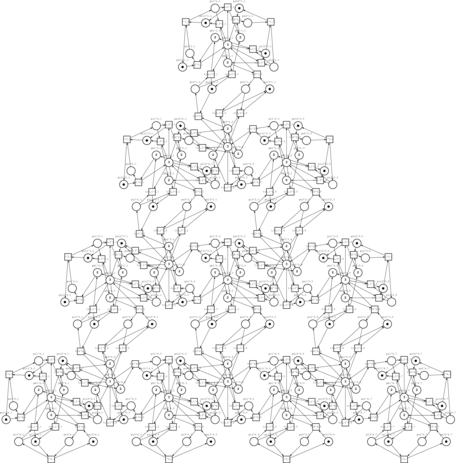
\includegraphics[width=8cm]{14_Shmeleva_fig1.png}
  \caption{~}
  \label{Shmeleva:fig1}
\end{figure}
\end{center}

\begin{center}
\begin{figure}[h!]
  \centering
  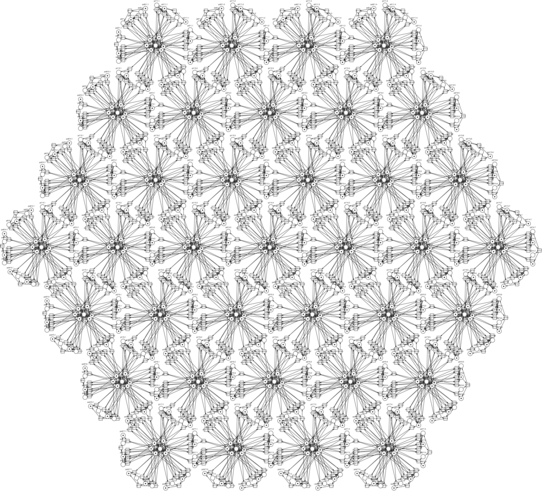
\includegraphics[width=8cm]{14_Shmeleva_fig2.png}
  \caption{~}
  \label{Shmeleva:fig2}
\end{figure}
\end{center}

An infinite Petri net is a powerful abstraction described in \cite{bib1} and \cite{bib2}, which allows the specification of models having an arbitrary size but a definite structure obtained by spatial composition of one or more basic components. An overwhelming result is obtained that gives a way to draw conclusions on properties of models with no regard to their size. For visualization and application of inductive methods which draw conclusions for infinite nets of definite structure, a fast facility that creates a model of a given size is required.

We developed a technique of software generators design based on the infinite Petri net specification and a series of about a dozen of generators of switching grid structure of square, triangular, and hexa\-gonal form on a plane (2D) as well as hypercube and hypertorus in multidimensional space listed in the Conclusions section. The open source software has been uploaded on GitHub and is compatible on data formats with modeling system Tina \cite{bib7}.

Modeling system Tina \cite{bib7} is for years de facto standard for Petri net models exchange and analysis; in 2019, Tina has won international Model Checking Contest. It allows automatic visualization of models, building its state space and finding structural properties \cite{bib5} as well as reflecting Petri net behavior --- token game.

\subsection*{Specification of Infinite Petri Nets}

The basic technique allows studying an infinite structures using their finite parametric specification obtained by repetition and composi\-tion of a single component. Our models are divided into two classes: for grids with definite number of dimensions, basically 1D and 2D; for grids with arbitrary number of dimensions. In the first case we use parameters of size only while in the second case a parameter which defines the number of dimensions is added. Structures having more than one basic component can be studied as well.

For majority of models we consider a cellular structure which implies connections of cells according to von Neumann neighborhood, some models are composed using Moore neighborhood, a generalized Zaitsev neighborhood is applied as well. Connection of neighbor cells is obtained by merging their contact places.

Remind that a Petri net is a bipartite directed graph supplied with dynamic elements called tokens. One part of vertices is called places and drawn as circles while the other part of vertices is called transitions and drawn as rectangles. We use notation of a parametric multiset rewriting system, each row specifies a transition by lists of its input and output places.

Let us consider a square grid specification obtained from a basic component represented by a single place as its repetition in cells of a two dimensional grid supplied by transitions according to von Neumann neighborhood written in TEX notation:

\begin{verbatim}
\begin{equation}\left(
\left(
\begin{array}{l}
t_{1,1}^{i,j}: p^{i,j} -> p^{i-1,j}, i>1,\\
t_{1,2}^{i,j}: p^{i,j} -> p^{i+1,j}, i<n,\\
t_{2,1}^{i,j}: p^{i,j} -> p^{i,j-1}, j>1,\\
t_{2,2}^{i,j}: p^{i,j} -> p^{i,j-1}, j<n,\\
\end{array}
\right),
1<=i<=n, 1<=j<=n, 
\right)
\end{equation}.\end{verbatim}
The parameter n gives the grid size while variables i and j specify the cell indices in horizontal and vertical directions correspondingly. The upper index (i,j) gives the cell location inside the lattice; i goes from top to down and j goes from left to right. Enumeration of transitions using two lower indices (d,r) suits multidimensional grid as well; d gives the number of dimension and r gives one of two directions: 1 -- to the origin, 2 -- to infinity.

\subsection*{Generators of Models in Logical Format}

Models in logical format are rather simple specifying names of places and transitions and their connections. Though for 2D models there is a definite lack of visibility, which is partially mended by automatic drawing a net by Tina, logical format is convenient for multidimensional grids where visualization is hampered.  The basic element of logical file format (.net) is the following:

\noindent{\small \verb@tr <t-name> <p-name>[*<weight>],… -> <p-name> [*<weight>],...@}

After the indicator “\verb!tr!”, the transition name follows, then a list of its input places, and after “\verb!\rightarrow{}!”, a list of its output places are written; optional arc weigh is started by “\verb!*!” sign, its absence means unary weight.  
The following fragment of C program generates the specified grid

\lstset{
  basicstyle=\ttfamily,
  columns=fullflexible,
  breaklines=true,
  postbreak=\mbox{\textcolor{red}{$\hookrightarrow$}\space},
}
\begin{lstlisting}[language=C]
for(i=1;i<=n;i++)
  for(j=1;j<=n;j++)
  {
      if(i>1) printf("tr {t_1,1^%d,%d} {p^%d,%d} -> {p^%d,%d}\n",i,j,i,j,i-1,j);
      if(i<n) printf("tr {t_1,2^%d,%d} {p^%d,%d} -> {p^%d,%d}\n",i,j,i,j,i+1,j);
      if(j>1) printf("tr {t_2,1^%d,%d} {p^%d,%d} -> {p^%d,%d}\n",i,j,i,j,i,j-1);
      if(j<n) printf("tr {t_2,2^%d,%d} {p^%d,%d} -> {p^%d,%d}\n",i,j,i,j,i,j+1);
  }\end{lstlisting}
Loaded into Tina, models are either visualized using “draw” tools or analyzed directly via calculating linear invariants and construction of reachability (coverability) tree. Inductive resoning on a series of basis invariants obtained for models of incremented size allow us obtaining invariants of infinite nets in parametric form.

\subsection*{Generators of Models in Graphical Format}

Models in graphical format are devised either for 2D or 1D grids. They reflect spatial structure of grid using coordinates of places and transitions. Some early models considered spatial structures of a single dimension, for instance for a bus Ethernet model. Among late one dimension models we constructed a generator of a net counting a double exponent. Basic models of a triangular, square, and hexagonal grids have been developed for a plane.

The peculiarity of graphical format is binding places and transitions of Petri nets to definite coordinated on plane. For simplicity we suppose arcs connecting nodes are straight though some our models contain curved arcs. At first we choose the grid cell size and compute a cell offset of its top-left corner on both coordinates; finally we add to the coordinates offsets inside cells. Having offsets DI and DJ, and supposing that a place is situated in the center of a cell having transitions in between with a space of 2DT in middle of two transitions with opposite direction of switching, we obtain the following code for printing a place and a transition of a cell:

\lstset{
  basicstyle=\ttfamily,
  columns=fullflexible,
  breaklines=true,
  postbreak=\mbox{\textcolor{red}{$\hookrightarrow$}\space},
}
\begin{lstlisting}[language=C]
printf("p %f %f {p^%d,%d} 0 n", i*DI, j*DJ, i, j);
printf("t %f %f  {to_1,1^%d,%d} 0 w n", i*DI-DT, j*DJ-DJ/2, i, j);
printf("e {p^%d,%d} {to_1,1^%d,%d} 1 n", i,j,i,j);
printf("e {to_1,1^%d,%d} {p^%d,%d} 1 n", i,j,i-1,j);\end{lstlisting}
Here in graphical format. a row started with: “p” specifies a place, “t” specifies a transition, and “e” specifies an arc; coordinates and a name follow for a node; an arc is given by two its ends; some additional parameters of graphical representation follow, for instance “0 w n”. 
As examples, images of triangular and hexagonal communication switching grids have been considered in the Introduction.

\subsection*{Conclusions}

The technique for software generators of Petri net models design is developed based on a given specification of an infinite Petri net. A series of open source generators have been implemented and uploaded on GitHub with MIT License for the following forms of grids:

\begin{itemize}
  \item square \url{https://github.com/dazeorgacm/sq};
  \item triangular \url{https://github.com/tishtri/g3a};
  \item hexagonal \url{https://github.com/tishtri/g6a};
  \item hypertorus \url{https://github.com/dazeorgacm/htgen};
  \item hypercube with various edge conditions \url{https://github.com/tishtri/hcgen};
  \item hypercube and hypertorus with generalized Zaitsev neighborhood \url{https://github.com/dazeorgacm/hmn}.
\end{itemize}

Converted by Tina \cite{bib7} to PNML format generated nets can be analysed using lots of open source software for Petri nets available on GitHub, say PNML\_Parse \cite{bib8}.

\begin{thebibliography}{9}
\bibitem{bib1} {Dmitry A. Zaitsev, Ivan D. Zaitsev and Tatiana R. Shmeleva. Infinite Petri Nets: Part 1, Modeling Square Grid Structures, Complex Systems, 26(2), 2017, 157-195.}
\bibitem{bib2} {Dmitry A. Zaitsev, Ivan D. Zaitsev and Tatiana R. Shmeleva. Infinite Petri Nets: Part 2, Modeling Triangular, Hexagonal, Hypercube and Hypertorus Structures, Complex Systems, 26(4), 2017, 341-371.}
\bibitem{bib3} {Grady Booch, The Unified Modeling Language User Guide. Addison Wesley Professional, 2017, 504p.}
\bibitem{bib4} {Zaitsev D.A., Jürjens J. Programming in the Sleptsov net language for systems control, Advances in Mechanical Engineering, 2016, Vol. 8(4), 1–11. http://dx.doi.org/10.1177/1687814016640159}
\bibitem{bib5} {ZhiWu Li, MengChu Zhou, Deadlock Resolution in Automated Manufacturing Systems: A Novel Petri Net Approach. Springer Science \& Business Media, 2009, 240p.}
\bibitem{bib6} {Zaitsev D.A. and Shmeleva T.R. Modeling With Colored Petri Nets: Specification, Verification, and Performance Evaluation of Systems (pp. 378-404) Chapter 14 in T. Shmelova, N. Rizun, D. Kucherov and K. Dergachov (Ed.) Automated Systems in the Aviation and Aerospace Industries. IGI-Global: USA, 2019.}
\bibitem{bib7} {Time Petri Net Analyzer (Tina), \url{http://projects.laas.fr/tina/}}
\bibitem{bib8} {Petri net from PNML file and build its reachability graph, \url{https://github.com/Tj-Cong/PNML_Parse}}
\end{thebibliography}
\end{document}

\documentclass[10pt, a5paper]{article}
\usepackage{pdfpages}
\usepackage{parallel}
\usepackage[T2A]{fontenc}
\usepackage{ucs}
\usepackage[utf8x]{inputenc}
\usepackage[polish,english,russian]{babel}
\usepackage{hyperref}
\usepackage{rotating}
\usepackage[inner=2cm,top=1.8cm,outer=2cm,bottom=2.3cm,nohead]{geometry}
\usepackage{listings}
\usepackage{graphicx}
\usepackage{wrapfig}
\usepackage{longtable}
\usepackage{indentfirst}
\usepackage{array}
\newcolumntype{P}[1]{>{\raggedright\arraybackslash}p{#1}}
\frenchspacing
\usepackage{fixltx2e} %text sub- and superscripts
\usepackage{icomma} % коскі ў матэматычным рэжыме
\PreloadUnicodePage{4}

\newcommand{\longpage}{\enlargethispage{\baselineskip}}
\newcommand{\shortpage}{\enlargethispage{-\baselineskip}}

\def\switchlang#1{\expandafter\csname switchlang#1\endcsname}
\def\switchlangbe{
\let\saverefname=\refname%
\def\refname{Літаратура}%
\def\figurename{Іл.}%
}
\def\switchlangen{
\let\saverefname=\refname%
\def\refname{References}%
\def\figurename{Fig.}%
}
\def\switchlangru{
\let\saverefname=\refname%
\let\savefigurename=\figurename%
\def\refname{Литература}%
\def\figurename{Рис.}%
}

\hyphenation{admi-ni-stra-tive}
\hyphenation{ex-pe-ri-ence}
\hyphenation{fle-xi-bi-li-ty}
\hyphenation{Py-thon}
\hyphenation{ma-the-ma-ti-cal}
\hyphenation{re-ported}
\hyphenation{imp-le-menta-tions}
\hyphenation{pro-vides}
\hyphenation{en-gi-neering}
\hyphenation{com-pa-ti-bi-li-ty}
\hyphenation{im-pos-sible}
\hyphenation{desk-top}
\hyphenation{elec-tro-nic}
\hyphenation{com-pa-ny}
\hyphenation{de-ve-lop-ment}
\hyphenation{de-ve-loping}
\hyphenation{de-ve-lop}
\hyphenation{da-ta-ba-se}
\hyphenation{plat-forms}
\hyphenation{or-ga-ni-za-tion}
\hyphenation{pro-gramming}
\hyphenation{in-stru-ments}
\hyphenation{Li-nux}
\hyphenation{sour-ce}
\hyphenation{en-vi-ron-ment}
\hyphenation{Te-le-pathy}
\hyphenation{Li-nux-ov-ka}
\hyphenation{Open-BSD}
\hyphenation{Free-BSD}
\hyphenation{men-ti-on-ed}
\hyphenation{app-li-ca-tion}

\def\progref!#1!{\texttt{#1}}
\renewcommand{\arraystretch}{2} %Іначай формулы ў матрыцы зліпаюцца з лініямі
\usepackage{array}

\def\interview #1 (#2), #3, #4, #5\par{

\section[#1, #3, #4]{#1 -- #3, #4}
\def\qname{LVEE}
\def\aname{#1}
\def\q ##1\par{{\noindent \bf \qname: ##1 }\par}
\def\a{{\noindent \bf \aname: } \def\qname{L}\def\aname{#2}}
}

\def\interview* #1 (#2), #3, #4, #5\par{

\section*{#1\\{\small\rm #3, #4. #5}}

\def\qname{LVEE}
\def\aname{#1}
\def\q ##1\par{{\noindent \bf \qname: ##1 }\par}
\def\a{{\noindent \bf \aname: } \def\qname{L}\def\aname{#2}}
}

\switchlang{en}
\begin{document}
\title{Case Study: Parallel Programming in Python with COMPSs}
\author{Nikolay Zaitsev, Odessa, Ukraine\footnote{\url{zaitsev.nikolay@rl.odessa.ua}, \url {https://lvee.org/ru/abstracts/300}}}
\maketitle
\begin{abstract}
An original made in European Union, namely in Barcelona Supercomputer Center, a system of parallel programming \linebreak COMPSs is studied on an example of parallelizing a simple program written in Python language. After annotating functions with the explicit specification of input and output information, COMPSs parallizes programs automatically with a function as a grain (job) of parallel process granulation. The COMPSs runtime system launches jobs dynamically on the readiness of their input data on available nodes (cores). The COMPSs system perfor\-mance is rather open issue which requires additional comparisons on test tasks with classical systems of parallel programming such as MPI and OpenMP.
\end{abstract}
\subsection*{1. Introduction}

Among parallel programming systems, generally accepted standards are: MPI for distributed nodes;  OpenMP for multi-core processors with shared memory; proprietary systems for graphics processors, such as CUDA for Nvidia graphics cards. All these systems require special approaches to the development of parallel programs. A programmer should plan numerous parallel branches and their complex interaction, which is often associated with additional errors.

The COMPSs system \cite{bib1} developed at the Barcelona Supercomputer Center is an open source system under the Apache License version 2. COMPSs provides a fundamentally new approach to parallel programming without parallel programming as such \cite{bib2}. The minimal ele\-ment of parallel processes granulation is a programming language func\-tion. The system COMPSs builds a graph of information connections of tasks and performs the dynamic launch of parallel processes on their readiness. This significantly reduces the complexity of developing parallel programs and ensures their correctness. The disadvantage of the COMPS system at its current experimental stage of its use is some instability and a relatively slow run-time system.

The Barcelona Supercomputing Center continues to improve the system by providing support for new programming languages; for exam\-ple, COMPSs currently supports the development of programs in such languages as C/C++, Java, and Python \cite{bib3}. Periodically, with the support of the European Union, schools and workshops take place on teaching programming technology within the COMPSs environment. One of such seminars was visited by the author in January 2019, where he received the corresponding certificate of the COMPSs programmer.

\subsection*{2. Principles of software development in COMPSs}

For automatic program parallelization, the COMPSs system builds a well-known graph of information connections. The key point in the construction of the information connections graph is an adequate choice of the granulation level of parallel processes. Work at the level of individual operators of a programming language is rather time consu\-ming and requires close integration with software of the compiler of a programming language.

To restrict the complexity of the implementation concept in \linebreak COMPSs, the principal decision was taken: the unit of parallelization is a function of the programming language. To build a graph of informati\-onal connec\-tions, it is necessary to know exactly which of the function parameters are either input or output (or both). In order not to analyze the program code of functions for making appropriate decisions, \linebreak COMPSs provides a special directive for annotation (decoration) of functions and some other program elements. From the point of view of the programming language, annotations are either special comments or directives of the compiler preprocessor. Besides, a small number of additional functions are used, for example, to synchronize processes.

\subsection*{3. A case study of developing a parallel program in the Python language}

Consider an example of a simple program that calculates the value of an arithmetic expression represented in Listing 1. For simplicity, there is no input of the source data to the program, initial values are assigned to the variables a and b. Listing \ref{NZ:lst1} also contains the command to start the program and the result of its computation.

\lstset{
  basicstyle=\ttfamily,
  columns=fullflexible,
  breaklines=true,
  postbreak=\mbox{\textcolor{red}{$\hookrightarrow$}\space},
}
\renewcommand{\lstlistingname}{Listing}

\begin{lstlisting}[language=Python,caption={~},label={NZ:lst1}]
a=2.2
b=3.3
y=a*b+a/b
print(y)
>python ab.py
7.92666666667
\end{lstlisting}
Analysis of the arithmetic expression allows us to assume that multipli\-cation and division operations can be performed in parallel in a multi\-processor environment (if there are at least two processors). To imple\-ment these operations in parallel, we modify the source program in such a way that: a) we specify each of the mentioned operations and also the addition operation as separate functions of the Python language; b) we use the superposition of functions to calculate the value of the source arithmetic expression. The resulting program, along with its launch command and the result of its work, is presented in Listing \ref{NZ:lst2}. Note that Listing 2 does not yet contain COMPS commands and is executed by the usual Python language environment. The results are the same.


\begin{lstlisting}[language=Python,caption={~},label={NZ:lst2}]
def mymul(x,y): return x*y
def myadd(x,y): return x+y
def mydiv(x,y): return x/y
a=2.2
b=3.3
z=myadd(mymul(a,b),mydiv(a,b))
print(z)
>python abf.py
7.92666666667\end{lstlisting}

Decorated for the COMPSs environment program, the command for launching it and the result of its execution are presented in Listing 3, the scheme of its execution follows fig. \ref{N:Zaitsev:fig1}.

The results coincide with the earlier considered results of the \linebreak previous two program variants. In such a simple case, we, of course, did not speed up the execution of the program by parallelizing it. However, when two parts of a big program, which are equal in complexity, are separated to functions, we will get about twice the acceleration of the execution time of these functions.


\begin{center}
\begin{figure}[h!]
  \centering
  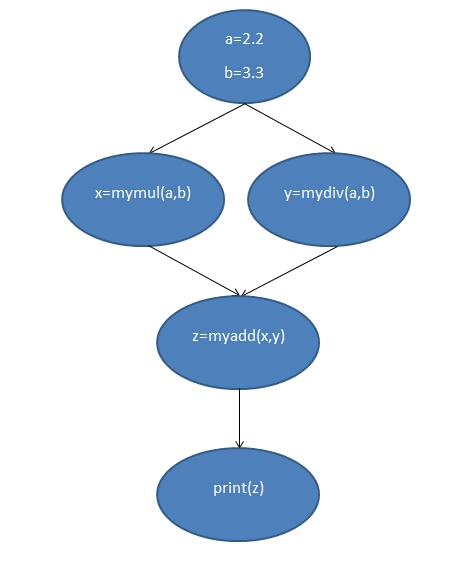
\includegraphics[width=9cm]{15_N_Zaitsev_fig1}
  \caption{~}
  \label{N:Zaitsev:fig1}
\end{figure}
\end{center}

\begin{lstlisting}[language=Python,caption={~},label={NZ:lst3}]
from pycompss.api.task import task	     # Import @task decorator
from pycompss.api.parameter import *	     # Import parameter metadata for the @task decorator
from pycompss.api.api import compss_wait_on  # Import synnchronization function
@task(x=IN, y=IN, returns=float)
def mymul(x, y):
    return x * y
@task(x=IN, y=IN, returns=float)
def myadd(x, y):
    return x + y
@task(x=IN, y=IN, returns=float)
def mydiv(x, y):
    return x/y
if __name__ == '__main__':
    a = 2.2
    b = 3.3
    z = myadd(mymul(a, b), mydiv(a, b))
    z = compss_wait_on(z)
    print(z)
>runcompss abfc.py
[  INFO] Using default execution type: compss
[  INFO] Using default location for project file: /opt/COMPSs/Runtime/configuration/xml/projects/default_project.xml
[  INFO] Using default location for resources file: /opt/COMPSs/Runtime/configuration/xml/resources/default_resources.xml
[  INFO] Inferred PYTHON language\end{verbatim}\begin{verbatim}----------------- Executing abfc.py --------------------------\end{verbatim}\begin{verbatim}WARNING: COMPSs Properties file is null. Setting default values
[(660)    API]  -  Starting COMPSs Runtime v2.5.rc1907 (build 20190702-1710.rb9d4035fbe39f8f3d692d485d359964971080cc0)
7.92666666667
[(4601)    API]  -  Execution Finished\end{lstlisting}
Let us consider the additional lines of the program prepared for exe\-cution by the COMPSs system. The \verb@from ... import ...@ directive describes the import of additional external facilities of the COMPSs system. The \verb@@task (...)@ decorator annotates the functions by specifying input parameters using the \verb@IN@ descriptor and the type of return value using the \verb@returns@ keyword. An expression for the conditional compi\-lation of the main program \verb@if __name__ == '__main__':@ was also added, as well as a call to the synchronization function \linebreak \verb@compss_wait_on (z)@ before printing the result \verb@z@. To run the program, we use the special command \verb@runcompss@.

Additional features of COMPSs, such as visualization of actual graphs of information connections, specification of cluster equipment, and project structure were left beyond the scope of this paper.

\subsection*{4. Conclusions}

The article presents a case study of the basic principles of programs parallelization in the system COMPSs on an example of calculating the arithmetic expression. In essence, it is necessary to add only one additional decoration line for each function declared in the program. Further program parallelization is performed automatically.

Comparisons of COMPSs efficiency with the traditional parallel programming technology such as MPI/OpenMP are rather vague at the present time. That is why the author invites submissions of applied software for various domains which is represented in both variants: a) a conventional program; b) a parallel program in MPI or (and) OpenMP. Comparisons of the obtained benchmarks for 3 cases: 1) conventional; 2) MPI/OpenMP; 3) COMPSs, -- will be reported to the next conference.

\subsection*{Literature}

\begin{thebibliography}{9}
\bibitem{bib1} {COMPSs source code \url{https://github.com/bsc-wdc/compss}}
\bibitem{bib2} {COMP Superscalar, an interoperable programming framework, SoftwareX, Volumes 3–4, December 2015, Pages 32–36, Badia, R. M., J. Conejero, C. Diaz, J. Ejarque, D. Lezzi, F. Lordan, C. Ramon-Cortes, and R. Sirvent, DOI: 10.1016/j.softx.2015.10.004}
\bibitem{bib3} {PyCOMPSs: Parallel computational workflows in Python, Enric Tejedor, Yolanda Becerra, Guillem Alomar, Anna Queralt, Rosa M. Badia, Jordi Torres, Toni Cortes, Jesús Labarta,  IJHPCA 31(1): 66-82 (2017), DOI: 10.1177/1094342015594678}\end{thebibliography}
\end{document}

\documentclass[10pt, a5paper]{article}
\usepackage{pdfpages}
\usepackage{parallel}
\usepackage[T2A]{fontenc}
\usepackage{ucs}
\usepackage[utf8x]{inputenc}
\usepackage[polish,english,russian]{babel}
\usepackage{hyperref}
\usepackage{rotating}
\usepackage[inner=2cm,top=1.8cm,outer=2cm,bottom=2.3cm,nohead]{geometry}
\usepackage{listings}
\usepackage{graphicx}
\usepackage{wrapfig}
\usepackage{longtable}
\usepackage{indentfirst}
\usepackage{array}
\newcolumntype{P}[1]{>{\raggedright\arraybackslash}p{#1}}
\frenchspacing
\usepackage{fixltx2e} %text sub- and superscripts
\usepackage{icomma} % коскі ў матэматычным рэжыме
\PreloadUnicodePage{4}

\newcommand{\longpage}{\enlargethispage{\baselineskip}}
\newcommand{\shortpage}{\enlargethispage{-\baselineskip}}

\def\switchlang#1{\expandafter\csname switchlang#1\endcsname}
\def\switchlangbe{
\let\saverefname=\refname%
\def\refname{Літаратура}%
\def\figurename{Іл.}%
}
\def\switchlangen{
\let\saverefname=\refname%
\def\refname{References}%
\def\figurename{Fig.}%
}
\def\switchlangru{
\let\saverefname=\refname%
\let\savefigurename=\figurename%
\def\refname{Литература}%
\def\figurename{Рис.}%
}

\hyphenation{admi-ni-stra-tive}
\hyphenation{ex-pe-ri-ence}
\hyphenation{fle-xi-bi-li-ty}
\hyphenation{Py-thon}
\hyphenation{ma-the-ma-ti-cal}
\hyphenation{re-ported}
\hyphenation{imp-le-menta-tions}
\hyphenation{pro-vides}
\hyphenation{en-gi-neering}
\hyphenation{com-pa-ti-bi-li-ty}
\hyphenation{im-pos-sible}
\hyphenation{desk-top}
\hyphenation{elec-tro-nic}
\hyphenation{com-pa-ny}
\hyphenation{de-ve-lop-ment}
\hyphenation{de-ve-loping}
\hyphenation{de-ve-lop}
\hyphenation{da-ta-ba-se}
\hyphenation{plat-forms}
\hyphenation{or-ga-ni-za-tion}
\hyphenation{pro-gramming}
\hyphenation{in-stru-ments}
\hyphenation{Li-nux}
\hyphenation{sour-ce}
\hyphenation{en-vi-ron-ment}
\hyphenation{Te-le-pathy}
\hyphenation{Li-nux-ov-ka}
\hyphenation{Open-BSD}
\hyphenation{Free-BSD}
\hyphenation{men-ti-on-ed}
\hyphenation{app-li-ca-tion}

\def\progref!#1!{\texttt{#1}}
\renewcommand{\arraystretch}{2} %Іначай формулы ў матрыцы зліпаюцца з лініямі
\usepackage{array}

\def\interview #1 (#2), #3, #4, #5\par{

\section[#1, #3, #4]{#1 -- #3, #4}
\def\qname{LVEE}
\def\aname{#1}
\def\q ##1\par{{\noindent \bf \qname: ##1 }\par}
\def\a{{\noindent \bf \aname: } \def\qname{L}\def\aname{#2}}
}

\def\interview* #1 (#2), #3, #4, #5\par{

\section*{#1\\{\small\rm #3, #4. #5}}

\def\qname{LVEE}
\def\aname{#1}
\def\q ##1\par{{\noindent \bf \qname: ##1 }\par}
\def\a{{\noindent \bf \aname: } \def\qname{L}\def\aname{#2}}
}

\switchlang{ru}
\begin{document}
\title{«Клиповое мышление» и универсальный инструмент создания интерактивных учебных материалов}
\author{Сергей Чоповский, Алла Чоповская, Львов, Ukraine\footnote{\url{auslemberg@meta.ua}, \url {https://lvee.org/ru/abstracts/307}}}
\maketitle
\begin{abstract}
Do I need a struggle with students' clip thinking? In order to overcome the negative trends in the development of the “digital generation”, the teacher needs to use modern computer technolo\-gies. One of such universal tools for creating interactive educati\-onal materials is the H5P project presented here.
\end{abstract}
Каждый, кто разрабатывает и внедряет учебные электронные ресурсы, со временем сталкивается с проблемою восприятия учебного материала «поколением гаджетов». Одной из таких проблем есть «клиповое мышление» \cite{bib1} — привычка воспринимать информацию с помощью короткого, яркого, очень выразительного образа. Если ранее учащиеся без особого труда сидели на уроке 45 минут, характер обучения был в основном линейным, теперь внимание учеников можно удерживать всего лишь 15 минут. «Поколение гаджетов» больше не желает читать толстые, скучные (написанные «сухим научным языком», где «многа букаф»), с невнятными иллюстрациями учебники. Информация поступает большими хаотичными потоками, у человека не остаётся достаточно времени для глубокого и сосредоточенного её анализа. Клиповое мышление — «фильтр», защищает мозг от информационных перегрузок.  Специалисты связывают его формирование с бурным развитием информационного пространства.

Нужна ли борьба с клиповым мышлением учеников \cite{bib2}?
Умение учителя приспособить учеников к изменившимся условиям современной жизни и использовать элементы клипового мышления для организации учебного процесса, важно научить учащихся мыслить глубоко (понятийно), уметь систематизировать информацию, анализировать её, использовать для принятия обоснованных решений. Тогда «клиповость» как элемент обучения будет присутствовать, но не преобладать. Для преодоления негативных тенденций развития «цифрового поколения», учителем необходимо использование современных компьютерных технологий (без злоупотребления оными).

Одним из таких универсальных инструментов создания интерактивных учебных материалов является проект H5P \cite{bib3}. Это основанная на JavaScript среда с открытым исходным кодом, предназначенная для совместной работы, создания и совместного использования интерактивного содержимого HTML5, распространяемая под лицензией MIT \cite{bib4}.

Платформа состоит из веб-редактора контента, веб-сайта для обмена типами контента, плагинов для существующих систем управления контентом и формата файлов для объединения ресурсов \linebreak HTML5. Сам сетевой редактор умеет добавлять и заменять мультимедийные файлы, текстовое содержимое во всех видах типов контента и приложений H5P. Имеются настраиваемые виджеты для редактора, обеспечивая любые возможности редактирования всех типов контента. 

\begin{center}
\begin{figure}[h!]
  \centering
  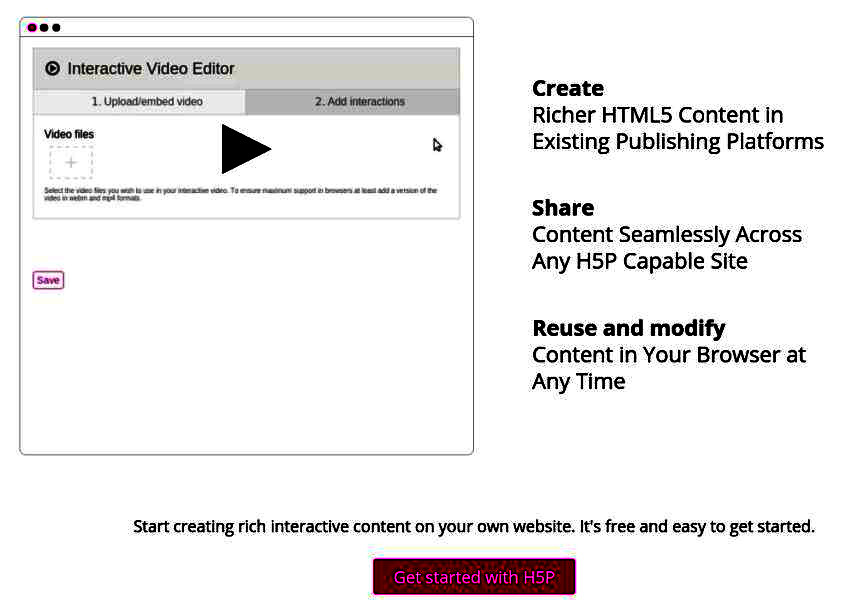
\includegraphics[width=10.8cm]{16_clip01}
  \caption{Фрагмент страницы h5p.org}
  \label{clip:fig1}
\end{figure}
\end{center}

Проект поддерживает кириллицу и снабжён хорошей справочной поддержкой. 

\begin{center}
\begin{figure}[h!]
  \centering
  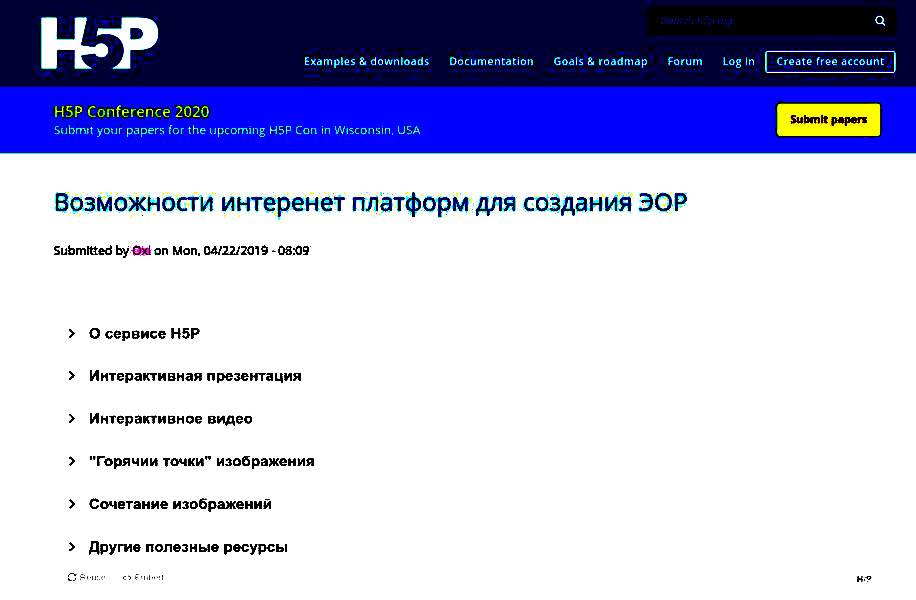
\includegraphics[width=10.8cm]{16_clip02}
  \caption{Фрагмент страницы О сервисе H5P}
  \label{clip:fig2}
\end{figure}
\end{center}

\begin{center}
\begin{figure}[h!]
  \centering
  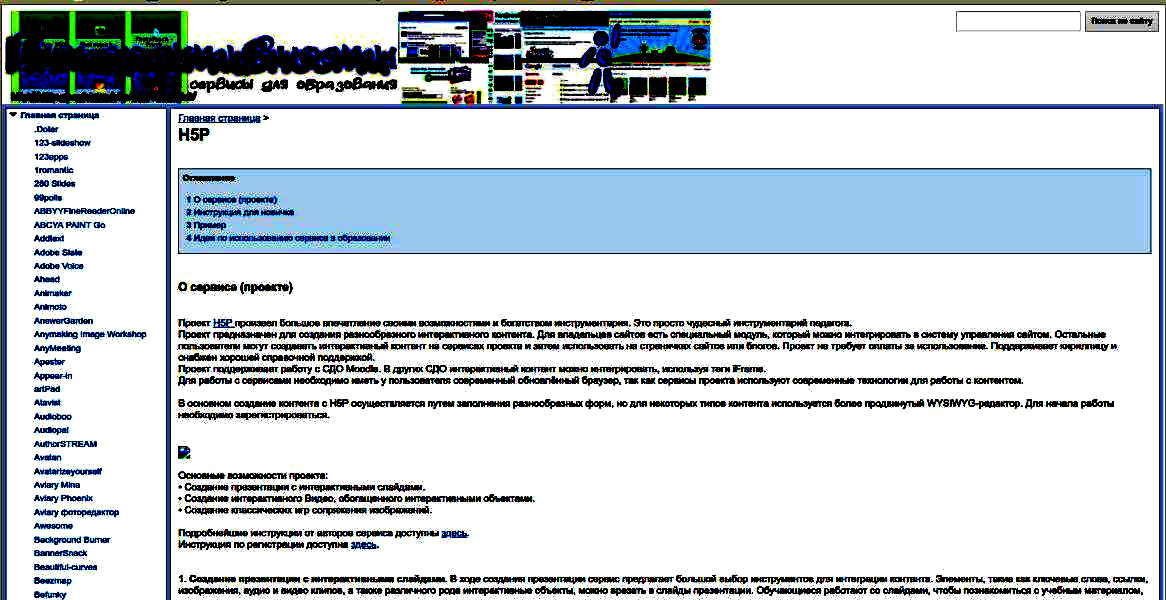
\includegraphics[width=10.8cm]{16_clip03}
  \caption{Интерактивности. Web-сервисы для образования}
  \label{clip:fig3}
\end{figure}
\end{center}

Так же проект поддерживает работу с системами ДО. Есть четыре основных плагина для Drupal, WordPress, Tiki и отдельно плагин для Moodle. В других СДО интерактивный контент можно использовать с помощью тега iFrame. Кроме выше перечисленных платформ, H5P удалось внедрить и использовать (через взаимодействие средств обучения—LTI Integration) в: Canvas (рис. \ref{clip:fig4}), Brightspace, Blackboard, LTI интеграция с Moodle, Интерактивный контент в Grav flat-file CMS,
в offline-редакторе HTML5 — \linebreak eXeLearning, добавление интерактивного контента в eXeLearning.


\begin{center}
\begin{figure}[h!]
  \centering
  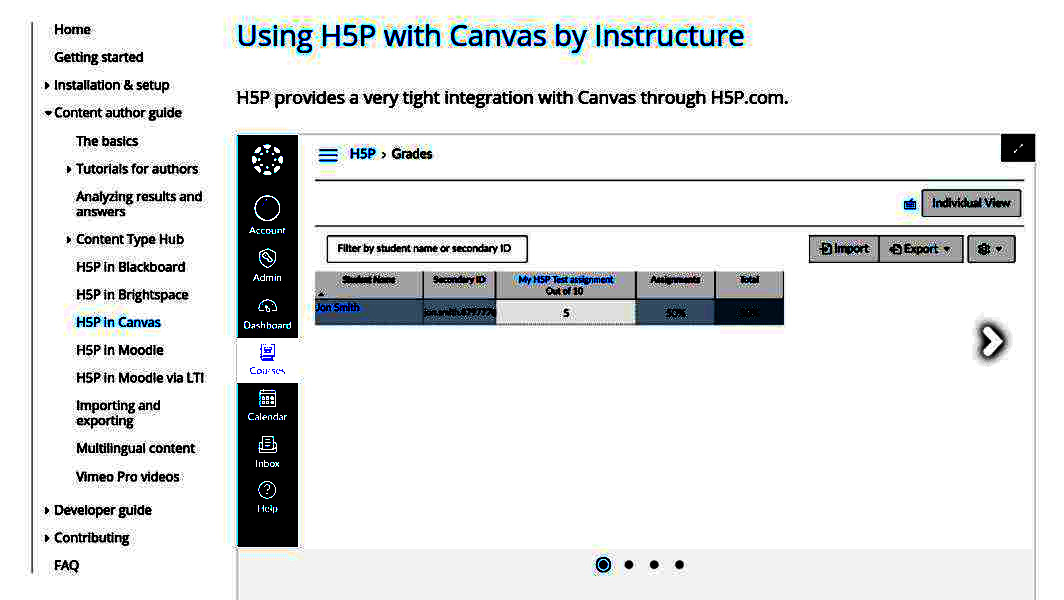
\includegraphics[width=10.8cm]{16_clip04}
  \caption{Интеграция с Canvas}
  \label{clip:fig4}
\end{figure}
\end{center} 

Кроме того H5P используется в качестве основного редактора разработки обучающего контента в diskurs LMS.
Для работы с сервисами необходимо иметь современный браузер совместимый с HTML5. Проект содержит более 40 шаблонов для создания электронных образовательных ресурсов. Основной язык проекта — английский, но большинство конструкторов в нем интуитивно понятны. И все разработки можно легко вставить на сайт или в блог. Интересно, что создание контента с H5P осуществляется путём заполнения разнообразных форм, для некоторых типов контента используется более продвинутый WYSIWYG-редактор. Рассмотрим основные возможности проекта \cite{bib5}:

\begin{itemize}
  \item Создание презентации с интерактивными слайдами: разнообразие тестовых заданий, ввод дополнительного контента, аналитические результаты тестирования, организация опроса.
  \item Создание интерактивного видео: разнообразие тестовых заданий, ввод комментариев, ввод дополнительного контента, возможность переключения к различным фрагментам видео, закладки, аналитические результаты тестирования, организация опроса.
  \item ``Горячие точки'' изображения: возможность акцентирования внимания на доступной области изображения, возможность ввода текста, изображения, видео, возможность показать изображение на большом экране.
  \item Создание классических игр сопряжения изображений: возможность увидеть объект, процесс, явление в разные периоды времени, стадии развития.
  \item Создание различных викторин: Baamboozle, Тривенты, \linebreak Myquiz.
\end{itemize}

\subsection*{Выводы}

«Клиповость»—это приобретённое качество, формируемое современными условиями существования и ритма жизни. При этом учащиеся не могут сосредоточиться, воспринимать длинные тексты, углубляться в суть, имеют крайне низкий коэффициент усвоения знаний. Неизбежность информатизации образования вызвана необходимостью использования больших объёмов информации во всех сферах деятельности и невозможностью формирования и обработки информации без помощи компьютерных технологий и средств связи.

Специалисты считают, что клиповое мышление – это не ущербность и не вина ученика, а естественный ответ на новые условия жизни. Клиповое мышление — это особенность мышления современного человека и это надо знать, чтобы помочь учащимся научиться мыслить полноценно. Для этого необходимо использовать комплексный подход, сочетая академические теоретические знания, наработку практических навыков в эксперименте и современные приёмы геймификации и мобильного обучения. Таким образом H5P (Библиотеки, приложении и типы контента) — это универсальный инструмент для создания интерактивных презентаций, видео, лент времени, плакатов, различных дидактических упражнений, опросов, игр и.т.п. Что позволяет фрагментарное представление информации увязывать с визуальными образами. При этом необходимо использовать метод дискуссий, который учит мыслить, отстаивать свою точку зрения и понимать противоположную, где поиск аргументации стимулирует логические процессы \cite{bib6}. 
Также надо использовать метод парадоксов —чтобы заставить ученика размышлять, а не просто пропускать через себя информацию. Отсутствие чётко сформулированной конечной мысли, готового вывода от учителя может заставить учащихся задуматься и задействовать логику. Приучать к чтению — научить учащихся самостоятельно выстраивать образную систему, где закрепление прочитанного (обсуждение, конспектирование и т.д.) способствует выработке умения анализировать, устанавливать связи между явлениями и, в конечном итоге, приводит к разрушению мозаичной, фрагментированной картины мира, тем самым помочь в преодолении негативных тенденций развития «цифрового поколения гаджетов».

А теперь немного фантазии: вероятно, что уже в недалёком будущем будут массово использоваться некие «обучающие машины». Скорее всего это будут «продвинутые» тренажёры (роботы) с ИИ, оснащённые аппаратурою дополненною реальностью. Их создание фактически идёт уже сейчас, и данный процесс с каждым днём все ускоряется. А вот и пример \cite{bib7}: В пресс-службе МТИ заявили, что в институте Робот-репетитор Алантим занимает должность зам.заведующего кафедрой робототехники. В будущем робот будет не только готовить учеников к экзаменам, но и проверять результаты ЕГЭ, используя искусственный интеллект. И что-то нам кажется, что и тут не обошлось без применения библиотек и приложений из H5P. Хотя несмотря на столь бурное развитие ИТ и ИИ, никакие «обучающие машины» не заменят полностью живого общения между учеником и учителем.

\begin{thebibliography}{9}
\bibitem{bib1} {{Клиповое мышление: чем отличаются «люди экрана» от «людей книги»?} \url{https://monocler.ru/klipovoe-myishlenie/}}
\bibitem{bib2} {{Клиповое мышление как фактор развития инновационных технологий в системе  образования}\url{https://znanio.ru/medianar/44/}}
\bibitem{bib3} {H5P -- Create and share rich HTML5 content and applications. \url{https://h5p.org/}}
\bibitem{bib4} {H5P is MIT Licensed. \url{https://h5p.org/MIT-licensed}}
\bibitem{bib5} {{Возможности интернет платформ для создания ЭОР}\url{https://h5p.org/node/489480}}
\bibitem{bib6} {{Клиповое мышление как проблема школьника, учителя, родителей}\url{https://en.ppt-online.org/376856}}
\bibitem{bib7} {{Робот-репетитор (МТИ) Алантим подготовит школьников к ЕГЭ}\url{https://vogazeta.ru/articles/2019/3/19/bigdata/6661-robot_repetitor_moskovskogo_tehnologicheskogo_instituta_podgotovit_shkolnikov_k_ege}}\end{thebibliography}
\end{document}

\documentclass[10pt, a5paper]{article}
\usepackage{pdfpages}
\usepackage{parallel}
\usepackage[T2A]{fontenc}
\usepackage{ucs}
\usepackage[utf8x]{inputenc}
\usepackage[polish,english,russian]{babel}
\usepackage{hyperref}
\usepackage{rotating}
\usepackage[inner=2cm,top=1.8cm,outer=2cm,bottom=2.3cm,nohead]{geometry}
\usepackage{listings}
\usepackage{graphicx}
\usepackage{wrapfig}
\usepackage{longtable}
\usepackage{indentfirst}
\usepackage{array}
\newcolumntype{P}[1]{>{\raggedright\arraybackslash}p{#1}}
\frenchspacing
\usepackage{fixltx2e} %text sub- and superscripts
\usepackage{icomma} % коскі ў матэматычным рэжыме
\PreloadUnicodePage{4}

\newcommand{\longpage}{\enlargethispage{\baselineskip}}
\newcommand{\shortpage}{\enlargethispage{-\baselineskip}}

\def\switchlang#1{\expandafter\csname switchlang#1\endcsname}
\def\switchlangbe{
\let\saverefname=\refname%
\def\refname{Літаратура}%
\def\figurename{Іл.}%
}
\def\switchlangen{
\let\saverefname=\refname%
\def\refname{References}%
\def\figurename{Fig.}%
}
\def\switchlangru{
\let\saverefname=\refname%
\let\savefigurename=\figurename%
\def\refname{Литература}%
\def\figurename{Рис.}%
}

\hyphenation{admi-ni-stra-tive}
\hyphenation{ex-pe-ri-ence}
\hyphenation{fle-xi-bi-li-ty}
\hyphenation{Py-thon}
\hyphenation{ma-the-ma-ti-cal}
\hyphenation{re-ported}
\hyphenation{imp-le-menta-tions}
\hyphenation{pro-vides}
\hyphenation{en-gi-neering}
\hyphenation{com-pa-ti-bi-li-ty}
\hyphenation{im-pos-sible}
\hyphenation{desk-top}
\hyphenation{elec-tro-nic}
\hyphenation{com-pa-ny}
\hyphenation{de-ve-lop-ment}
\hyphenation{de-ve-loping}
\hyphenation{de-ve-lop}
\hyphenation{da-ta-ba-se}
\hyphenation{plat-forms}
\hyphenation{or-ga-ni-za-tion}
\hyphenation{pro-gramming}
\hyphenation{in-stru-ments}
\hyphenation{Li-nux}
\hyphenation{sour-ce}
\hyphenation{en-vi-ron-ment}
\hyphenation{Te-le-pathy}
\hyphenation{Li-nux-ov-ka}
\hyphenation{Open-BSD}
\hyphenation{Free-BSD}
\hyphenation{men-ti-on-ed}
\hyphenation{app-li-ca-tion}

\def\progref!#1!{\texttt{#1}}
\renewcommand{\arraystretch}{2} %Іначай формулы ў матрыцы зліпаюцца з лініямі
\usepackage{array}

\def\interview #1 (#2), #3, #4, #5\par{

\section[#1, #3, #4]{#1 -- #3, #4}
\def\qname{LVEE}
\def\aname{#1}
\def\q ##1\par{{\noindent \bf \qname: ##1 }\par}
\def\a{{\noindent \bf \aname: } \def\qname{L}\def\aname{#2}}
}

\def\interview* #1 (#2), #3, #4, #5\par{

\section*{#1\\{\small\rm #3, #4. #5}}

\def\qname{LVEE}
\def\aname{#1}
\def\q ##1\par{{\noindent \bf \qname: ##1 }\par}
\def\a{{\noindent \bf \aname: } \def\qname{L}\def\aname{#2}}
}

\switchlang{ru}
\begin{document}
\title{Измеряем океан мензуркой (оценка характеристик глобальной сети)}
% \author{Александра Кононова, Moscow/Zelenograd, Russian Federation, \linebreak Алексей Городилов, Russian Federation} % не лезет!
\author{Александра Кононова, Алексей Городилов, \\ Russian Federation\footnote{\url{illinc@bk.ru}, \url{https://lvee.org/ru/abstracts/317}}}
\maketitle
\begin{abstract}
% Описан эксперимент по оцениванию распределения длин путей между узлами в~глобальной сети и~его характеристик.
% В~частности, показана методика измерения длины пути от узла $\alpha$ к узлу $\beta$ при помощи утилиты GNU/Linux traceroute и~ограничения выбора узлов $\alpha$ и~$\beta$, налагаемые этим инструментом.
% Приведены результаты измерений.
% Описана имитационная модель эксперимента, разработанная для проверки корректности полученных оценок распределения длин путей между узлами в~глобальной сети.
% Показано, что глобальная сеть не описывается моделью Барабаши"--~Альберт, но может быть в~некотором приближении описана разработанной  предфрактальной моделью.
The experiment, aimed at finding the distribution of path lengths between nodes in the global network and estimation of parameters of that distribution is described. 
At particular, described the method of measurement of path length from node $\alpha$ to the node $\beta$ with traceroute utility of the GNU/Linux system, and limitations on the selection of nodes $\alpha$ and $\beta$, imposed by trace\-route.
Measurements results are given and analyzed.
Simulation model of this experiment was developed to test the experiment validity in the determination of distribution parameters in the global network. This model is also described. 
It is shown that the global network could not be described by Barab\'{a}si-Albert model, but it could be described with some approximation by developed and proposed a pre-fractal model.
\end{abstract}

\subsection*{Введение}


Разработка эффективных сетевых приложений невозможна без сведений о структуре сети, в которой они будут работать. Так, в 2011 году, для получения параметров методики МУчОС~\cite{muchos} передачи мультимедийных данных с учётом особенностей сети, был начат эксперимент по оценке распределения длин путей  сетевого уровня модели TCP/IP глобальной сети.

Определим понятие длины пути и~распределения длин путей.
Из-за 
% особенностей 
свойств
стека протоколов TCP/IP, если от узла $\alpha$ к узлу $\beta$ в~принципе возможна передача данных,  маршрут передачи данных на сетевом уровне будет единственным.
Пусть это $\alpha \to \alpha_1 \to \ldots \to \alpha_{k-1} \to \beta$. 

% Тогда количество $k$ пересылок узел-узел в этом маршруте будем называть длиной пути от узла $\alpha$ к узлу $\beta$:
% $$
% s(\alpha, \beta) = k,
% $$

Тогда длина  $s(\alpha, \beta)$ пути от узла $\alpha$ к узлу $\beta$ "--- количество $k$ пересылок узел-узел в этом маршруте.
При этом $s(\alpha_{k-1}, \beta) = 1$, ...  $s(\alpha_1, \beta) = k-1$.

Со временем глобальная сеть изменяет свою структуру, и как маршрут передачи данных, так и~его длина $s(\alpha, \beta)$ могут изменяться.
Кроме того,
из-за особенностей маршрутизации может быть $s(\alpha, \beta) \neq s(\beta, \alpha)$.
% ; кроме того, как $s(\alpha, \beta)$, так и маршрут передачи данных от $\alpha$ к $\beta$ может изменяться во времени. При этом в каждый момент времени $s(\alpha_1, \beta) = s(\alpha, \beta) - 1$ и т. д.

Таким образом, под распределением длин путей графа $G$ 
понимается ряд чисел $\zeta(x)$, показывающий, как часто длина $x$ встречается среди всех возможных путей в~$G$:
$$
\zeta(x) = p \big(
s(\alpha,\beta)=x ~ | ~ \alpha,\beta \in G
\big).
$$
Непосредственно измерить распределение длин путей $\zeta(x)$ для глобальной сети (то есть измерить и~проанализировать длины $s(\alpha, \beta)$ для всех возможных пар $(\alpha, \beta)$) невозможно как из-за её гигантских размеров, так и~из-за отсутствия в~стеке TCP/IP средств для измерения расстояния между двумя произвольно взятыми узлами.


\subsection*{Выбираем мензурку}

Для исследования маршрутов сетевого уровня в~GNU/Linux \linebreak предназначена утилита traceroute.
При запуске в~командной строке узла $\alpha$ команды \mbox{\texttt{traceroute $\beta$}} результатом будет маршрут передачи данных $\alpha \to \alpha_1 \to \ldots \to \alpha_{k-1} \to \beta$, причём одна строка вывода traceroute соответствует одному узлу маршрута.
Далее путём синтаксического анализа можно определить длину пути $s(\alpha, \beta)$.

Таким образом, для измерения длины пути $s(\alpha, \beta)$  необходимо иметь право на запуск программ на узле 
$\alpha$ (в~дальнейшем будем называть его корневым, рис.~\ref{ei_rdp}) и~знать IP-адрес или имя узла  $\beta$ (будем называть его оконечным).
\begin{figure}[h!]
  \centering
  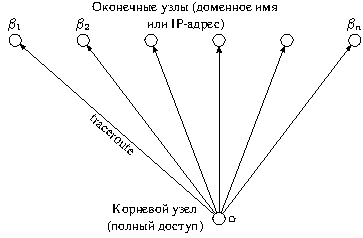
\includegraphics[width=0.7\linewidth]{2019_miet_kai_gav_ei_rdp}
\caption{Схема измерений выборочных длин путей}
\label{ei_rdp}
\end{figure}%
Также необходима возможность соединения $\alpha$ с~$\beta$, то есть оконечный узел $\beta$ должен иметь белый IP-адрес либо находиться в~одной подсети с~$\alpha$.

Ограничения на выбор оконечного узла гораздо мягче, чем для корневого.
Соответственно, количество возможных оконечных узлов может быть намного больше (множество оконечных узлов $Q=\{\beta_1, \beta_2, \ldots \beta_n \}$ на рис.~\ref{ei_rdp}).



Соответственно, задавшись парой из корневого узла $\alpha$ и~множества оконечных узлов $Q$ и~измеряя при помощи traceroute расстояния $s(\alpha, \beta_j)$ от 
$\alpha$ до каждого из оконечных $\beta_j \in Q$, можно получить 
% долю путей 
некоторую оценку распределения длин путей $\zeta(x)$ глобальной сети.
Эта оценка зависит от выбора корневого узла, от множества оконечных узлов и~от времени (от текущей конфигурации глобальной сети).


%Соответственно, граф, вершинами которого являются все доступные узлы глобальной сети (с белыми IP-адресами), а рёбрами "--- ???, является деревом.
В ходе этого эксперимента были сформированы три различных множества оконечных узлов ($P, R, T$ размерами  564, 5222 и~540 уникальных белых IP-адресов соответственно)
и~три корневых узла ($A, H, M$).


Так как все оконечные узлы имели белые IP-адреса, а~корневые "--- серые,
каждый маршрут передачи данных $\alpha \to \alpha_1 \to \ldots \to \alpha_{k-1} \to \beta$
от корневого узла $\alpha$ до оконечного узла $\beta$ делился на две части:
 маршрут от корневого узла $\alpha$ до шлюза $\alpha_{gw}$ его провайдера $\alpha \to \ldots \to \alpha_{gw}$
и~маршрут от шлюза провайдера корневого узла до оконечного узла $\alpha_{gw}\to \ldots\to \alpha_{k-1} \to \beta$.

Для каждой пары корневого узла $\alpha$ и~оконечного узла $\beta$ получались два значения длины пути:
полная длина $\widetilde{s}(\alpha, \beta) = k$, включающая подсеть  провайдера корневого узла
и~скорректированная длина ${s}(\alpha, \beta) = k-gw$, исключающая подсеть  провайдера корневого узла (то есть включающая только пересылки между узлами с~белыми IP-адресами).

После окончания измерений множества полученных значений длин путей $\widetilde{s}$ и~$s$ обрабатывались GNU Octave.
% 
Соответственно, для каждой пары корневого узла $\alpha$ и~множества оконечных узлов $Q$ получались две оценки распределения длин путей:
$\widetilde{\zeta}(x)$, включающая подсеть  провайдера корневого узла
и~$\zeta(x)$, исключающая подсеть  провайдера корневого узла.


\subsection*{Оцениваем}

От корневых узлов $A$ и~$M$ было выполнено по четыре разнесённых во времени измерения расстояний до каждого из наборов $P$, $R$, $T$;
от узла $H$, из-за ограниченного времени доступа "--- только по одному измерению до каждого из наборов $P$, $R$, $T$.
Таким образом, всего было выполнено 27~измерений и~получено 27 оценок $\widetilde{\zeta}(x)$ распределения длин путей, включающих подсеть провайдера корневого узла (рис.~\ref{zplot_2x1}, а)
\begin{figure}[h!]
  \centering
  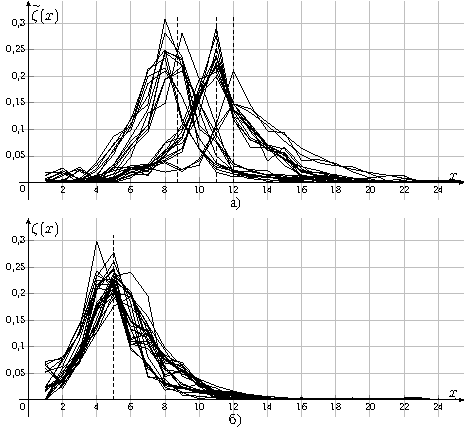
\includegraphics[width=\linewidth]{2019_miet_kai_gav_zplot_2x1}
\caption{Экспериментально полученное распределение длин путей:
а) включая подсеть провайдера корневого узла,
б)~исключая подсеть провайдера корневого узла
}
\label{zplot_2x1}
\end{figure}%
и~27 оценок~$\zeta(x)$ распределения длин путей, исключающих подсеть провайдера корневого узла (рис.~\ref{zplot_2x1}, б).

В~соответствии с~множеством оконечных узлов, корневым узлом и~порядковым номером измерения
обозначены как $PA_0, PA_1, PA_2,$ $PA_3,$ $PH_0, PM_0, \ldots PM_3,$ $RA_0, \ldots RM_3, TA_0, \ldots TM_3$
и~перечислены на рис.~\ref{5x2_experiment_moments} именно в~таком порядке.

\begin{figure}[p]
  \centering
  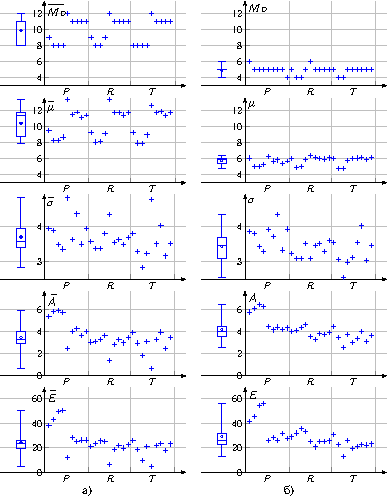
\includegraphics[width=\linewidth]{2019_miet_kai_gav_5x2_experiment_moments}
\caption{Характеристики экспериментально полученных оценок распределения длин путей:
а) включая подсеть провайдера корневого узла,
б)~исключая подсеть провайдера корневого узла
}
\label{5x2_experiment_moments}
\end{figure}

Рис.~\ref{5x2_experiment_moments}, а) показывает разброс характеристик (моды $Mo$, среднего $\mu$, среднеквадратического отклонения $\sigma$, асимметрии $A$ и~эксцесса $E$) оценок $\widetilde{\zeta}(x)$ распределения длин путей, включающих подсеть провайдера корневого узла.
% По оси абсцисс 
Ось абсцисс соответствует номеру измерения, как сказано выше; 
% измерения сгруппированы по множеству оконечных узлов ($P$, $R$, $T$ "--- границы групп показаны линиями сетки), затем по корневому узлу
% % , внутри каждой группы упорядочены по 
% и~времени ($A_0$, $A_1$, $A_2$, $A_3$, далее $H_0$ и~$M_0$, $M_1$, $M_2$, $M_3$).
границы между измерениями, соответствующими множествам оконечных узлов $P$, $R$, $T$  показаны линиями сетки.
% 
Слева от оси ординат разброс показан в~виде ящика с~усами (усы соответствуют минимальному и~максимальному значениям, края ящика "--- первой и~третьей квартилям, линия внутри ящика "--- медиане, кружок "--- среднему значению характеристики).
 
Рис.~\ref{5x2_experiment_moments}, б) аналогично показывает разброс характеристик оценок $\zeta(x)$ распределения длин путей, исключающих подсеть провайдера корневого узла.

Значение эксцесса $E$ здесь и~далее вычисляется по формуле с~коррекцией на три (так, чтобы эксцесс нормального распределения был бы равен нулю).

Видно, что значения асимметрии и~эксцесса оценок распределения длин путей (как $\widetilde{\zeta}(x)$, так и~$\zeta(x)$) существенно больше нуля.

\subsection*{Поверяем}

Насколько корректны полученные оценки $\zeta(x)$?
% 
Для их проверки было сгенерировано некоторое количество графов $G$, размеры которых позволяют:
\begin{itemize}
	\item[--]рассчитать расстояние $s(\alpha, \beta)$ для всех возможных пар узлов $\alpha, \beta \in G$ и~рассчитать истинное (полное) распределение длин путей $\zeta(x)$;
	
	\item[--] %а~также 
	выполнить имитацию эксперимента и~оценить  $\zeta(x)$ по 
заданным корневому узлу $r$ и~множеству оконечных узлов $Q$.
\end{itemize}
Размеры множеств $Q$, использованных в~экспериментальном исследовании, составляют $500-5000$ узлов.
Соответственно, минимальным количеством вершин в~$G$ в~расчётах было $|G| = 10^3$ узлов.
Максимальным размером $G$, при котором можно выполнить расчёт менее чем за месяц "--- $|G| = 10^6$ узлов.

Граф $G$ из~$|G|$ вершин представлялся в~памяти компьютера в~виде сжатой матрицы смежности,
то есть вектором $\rho_G$ из~$|G|$ списков,
каждый из которых соответствует вершине графа  и~содержит номера смежных с~ней вершин.
% Таким образом, элемент вектора $\rho_G$ с~номером $i \in [0, |G|)$ соответствует вершине $\nu_i$ и~хранит список вершин, смежных с~$\nu_i$.

% Как для расчёта 
Для расчёта длин путей использован  поиск в~ширину,
позволяющего для заданной вершины  $\alpha \in G$ рассчитать расстояния до всех прочих вершин графа $G$.
Таким образом, результат соответствует экспериментальным измерениям для корневой вершины $\alpha$ и~множества оконечных вершин $Q=G$, включающего все вершины графа.
Сложность поиска в~ширину для представления графа в~виде $\rho_G$  равна $O(|G| +|E_G|)$, где $|E_G|$ "--- количество рёбер~\cite{Sedgewick2002_AlgorithmsinC_Fundamentals}.
Таким образом, при расчёте полного распределения длин путей все вершины $\alpha \in G$ графа  поочерёдно рассматриваются в~качестве корневых, и~сложность возрастает в~$|G|$ раз.
Для ускорения расчёта  использован компилируемый язык C++ (стандарт C++11) и~распараллеливание OpenMP.

Кроме полного распределения длин путей $\zeta(x)$, для каждого графа $G$ рассчитывались ещё 
% Для каждого дерева $G$ рассчитывалось как полное распределение длин путей $\zeta(x)$, так  и~
несколько оценок $\zeta(x)$ по разным парам  $(r,Q)$ корневой узел-множество оконечных узлов. 
Эти оценки обозначались $\zeta_i(x)$.
%  , где $i$ "--- порядковый номер .

Корневая вершина $r$, как и~оконечные вершины $\beta_j \in Q$ для каждого $i$ выбиралась случайно.
Количество оконечных вершин $|Q|$ во время предварительных вычислений варьировалось в~диапазоне $500-5000$ узлов.
Так как не было выявлено существенного различия результатов, для итогового моделирования было принято $|Q|=500$.

Таким образом, аналогом выполненных в~эксперименте измерений (оценивания распределения длин путей глобальной сети по нескольким корневым узлам и~нескольким выборкам оконечных узлов)
является один прогон модели, включающий
% :
% \begin{itemize}
% 	\item[--] 
% \end{itemize}
генерацию графа $G$ (модели сети), расчёт полного распределения длин путей $\zeta(x)$ в~нём и~его оценок $\zeta_i(x)$ (моделей экспериментальных оценок).
Вид полного $\zeta(x)$ и~его оценок $\zeta_i(x)$ для одного из прогонов модели представлен на рис.~\ref{rdp_fullpart_ba}).

\begin{figure}[!h]
  \centering
  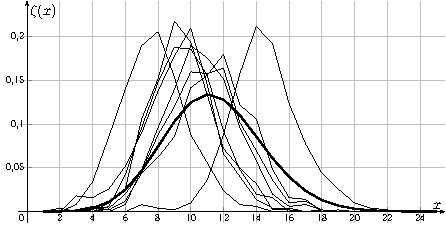
\includegraphics[width=\linewidth]{2019_miet_kai_gav_rdp_fullpart_ba}
  \caption{Распределение длин путей  между узлами (жирная линия "--- полное $\zeta(x)$, тонкие "--- его оценки~$\zeta_i(x)$) в~дереве  Барабаши"--~Альберт} 
\label{rdp_fullpart_ba}
\end{figure}

Целью вычислительного эксперимента является сопоставление полного $\zeta(x)$ и~его оценок~$\zeta_i(x)$, а~также их характеристик,
в~частности, асимметрии и~эксцесса.

Так как  граф $G$ является моделью сетевого уровня сети, использующей стек протоколов TCP/IP,
% Для наилучшего соответствия сетевому уровню сети TCP/IP 
$G$ должен быть связным деревом.
Сложность поиска в~ширину для дерева составляет $O(|G|)$, таким образом, сложность расчёта всех возможных путей составляет $O(|G|^2)$.


Были использованы несколько алгоритмов для генерации связного дерева $G$.
Прежде всего исследована знаменитая модель Барабаши"--~Альберт~\cite{ba} (типичные результаты прогона модели, то есть полное $\zeta(x)$ и~его оценки, показаны на рис.~\ref{rdp_fullpart_ba}).
% На рис.~\ref{rdp_fullpart_ba} показан типичный пример графика $\zeta(x)$ (жирная линия) и~$\zeta_{i}(x)$ (множество тонких линий) РДП для модели Барабаши"--~Альберт.

Полное $\zeta(x)$ для деревьев Барабаши"--~Альберт очень похоже на дискретизацию нормального.
Все они унимодальны.
Большинство оценок $\zeta_i(x)$ рис.~\ref{rdp_fullpart_ba} выглядит более островершинными, чем полное $\zeta(x)$, но менее островершинными, чем распределения, полученные экспериментально (рис.~\ref{zplot_2x1}, а, б).
Рассмотрим характеристики полных распределений и~их оценок подробнее (рис.~\ref{5_moments_ba}).

\begin{figure}[p]
  \centering
  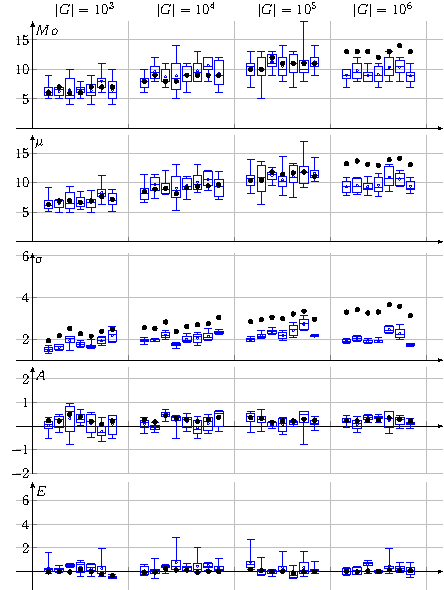
\includegraphics[width=\linewidth]{2019_miet_kai_gav_5_moments_ba}
\caption{Характеристики полного  распределения длин путей в~дереве  Барабаши"--~Альберт (чёрные точки) и~разброс характеристик  его оценок (ящики с~усами)}
\label{5_moments_ba}
\end{figure}

Так как один прогон модели соответствует множеству 
% экспериментальных измерений,  
оценок, а~в~процессе исследования было выполнено множество прогонов, визуализировать характеристику каждой конкретной оценки аналогично рис.~\ref{5x2_experiment_moments} нерационально.
Соответственно, один прогон на рис.~\ref{5_moments_ba} соответствует одной вертикали (по оси абсцисс откладывается номер смоделированного графа; измерения сгруппированы по количеству $|G|$ вершин в~графе).
Для каждого прогона и~каждой характеристики показан разброс значений характеристики $\zeta_i(x)$ в~виде ящика с~усами (аналогично показанному слева на рис.~\ref{5x2_experiment_moments});
кроме того, чёрной точкой на рис.~\ref{5_moments_ba} показано значение характеристики $\zeta(x)$ (для экспериментальных данных его аналог "--- характеристика $\zeta(x)$ глобальной сети "--- недоступна и~поэтому отсутствует на рис.~\ref{5x2_experiment_moments}).

Видно, что асимметрия полных распределений $\zeta(x)$ для деревьев Барабаши"--~Альберт несколько больше нуля, но не достигает полученных в~результате эксперимента значений $3-4.5$.
Асимметрия оценок $\zeta_i(x)$ может быть как больше, так и~(что чаще) ещё меньше асимметрии $\zeta(x)$.
С~ростом количества $|G|$ вершин в~графе  асимметрия как $\zeta(x)$, так и~$\zeta_i(x)$ не растёт.

Эксцесс полных распределений $\zeta(x)$ для деревьев Барабаши"--~Альберт близок к нулю.
Эксцесс оценок $\zeta_i(x)$ может быть как больше (что чаще), так и~меньше эксцесса $\zeta(x)$,
при этом ни одна из этих величин не достигает полученных в~результате эксперимента значений $20-30$.
С~ростом количества $|G|$ вершин в~графе  эксцесс как $\zeta(x)$, так и~$\zeta_i(x)$ не растёт.

Погрешность оценивания асимметрии достигает 100\%, а~эксцесса "--- 1000\% (последнее обусловлено близостью к~нулю эксцесса  $\zeta(x)$).


Таким образом, различие между асимметрией и~эксцессом экспериментально полученных для сетевого уровня глобальной сети данных и~распределениями длин путей в~деревьях Барабаши"--~Альберт обусловлено не случайными отклонениями, не методикой измерения
и~не отличием в~размерах (асимметрия и~эксцесс мало изменяются при росте $|G|$).

Соответственно, различие должно быть обусловлено моделью роста дерева.
В~исследовании были рассмотрены несколько моделей роста.
Наиболее перспективной выглядит предфрактальная модель, описывающая рост сети как рост множества связанных друг с~другом подсетей (рис.~\ref{rdp_fullpart_pfk_32} и~\ref{6_moments_pfk_32}).

\begin{figure}[!h]
  \centering
  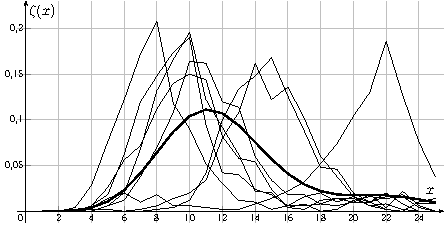
\includegraphics[width=\linewidth]{2019_miet_kai_gav_rdp_fullpart_pfk_32}
  \caption{Распределение длин путей между узлами (жирная линия "--- полное $\zeta(x)$, тонкие "--- его оценки~$\zeta_i(x)$) в~предфрактальном дереве} 
\label{rdp_fullpart_pfk_32}
\end{figure}

\begin{figure}[p]
  \centering
  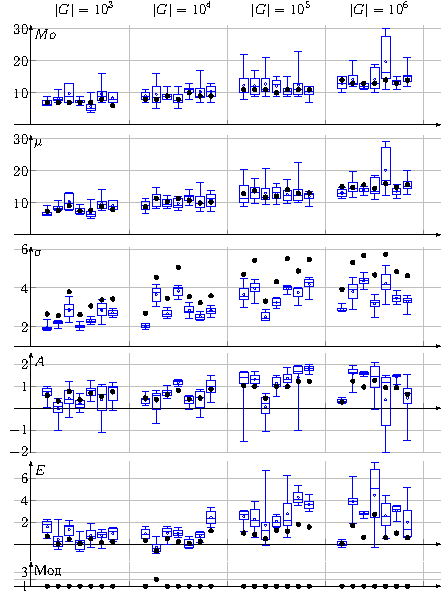
\includegraphics[width=\linewidth]{2019_miet_kai_gav_6_moments_pfk_32}
\caption{Характеристики полного распределения длин путей в~предфрактальном дереве (чёрные точки) и~разброс характеристик его оценок (ящики с~усами)}
\label{6_moments_pfk_32}
\end{figure}%

Вид полного $\zeta(x)$ и~его оценок $\zeta_i(x)$ для одного из прогонов модели представлен на рис.~\ref{rdp_fullpart_pfk_32}.
На рис.~\ref{6_moments_pfk_32} этот прогон "--- первый в~группе $|G|=10^5$.

Так как подсети формируются при росте графа случайным образом,
полные $\zeta(x)$ для предфрактальных деревьев более разнообразны, чем для деревьев Барабаши"--~Альберт.
Некоторые из них не унимодальны.
Соответственно, на рис.~\ref{6_moments_pfk_32}
в~числе прочих характеристик показано и~количество выраженных максимумов $\zeta(x)$.
В~остальном организация рис.~\ref{6_moments_pfk_32} аналогична рис.~\ref{5_moments_ba}.

Распределение $\zeta(x)$ на рис.~\ref{rdp_fullpart_pfk_32} отличается от рис.~\ref{5_moments_ba} наличием толстого правого хвоста.
% ,
% % который, хотя и~не формирует 
% Это "--- наиболее типичная форма $\zeta(x)$ предфрактального дерева.
% Тем не менее, в~зависимости от соотношения размеров подсетей $\zeta(x)$ может иметь
В~целом, в~зависимости от соотношения размеров подсетей 
% % а~также соединений 
$\zeta(x)$ предфрактального дерева может иметь как более или менее толстый правый хвост, аналогичный рис.~\ref{rdp_fullpart_pfk_32}, так и~
один или несколько ярко выраженных побочных максимумов (второй прогон в~группе $|G|=10^5$), либо, наоборот, может иметь тонкий хвост, как для $\zeta(x)$  деревьев Барабаши"--~Альберт (первый прогон в~группе $|G|=10^6$ "--- в~процессе роста сформировалась только одна крупная подсеть).

Соответственно, разброс как характеристик $\zeta(x)$ для разных прогонов, так и~их оценок $\zeta_i(x)$ для одного прогона модели на~рис.~\ref{6_moments_pfk_32} больше, чем на~рис.~\ref{5_moments_ba}.

Асимметрия и~эксцесс $\zeta(x)$ первого прогона в~группе $|G|=10^6$ (с~единственной крупной подсетью) ожидаемо близки к~асимметрии и~эксцессу $\zeta(x)$  деревьев Барабаши"--~Альберт, а~их оценки имеют столь же маленький разброс.

Асимметрия полного $\zeta(x)$ второго прогона в~группе $|G|=10^5$ (с~двумя конкурирующими подсетями, то есть практически одинаковыми максимумами) положительна, 
при этом асимметрии её оценок могут принимать и~отрицательные значения.
Эксцесс полного $\zeta(x)$ и~большинство его оценок отрицательны, так как два близких максимума суммарно массивнее хвостов распределения.

Для всех прочих прогонов асимметрия и~эксцесс положительны, а~их оценки в~подавляющем большинстве завышены.
При этом с~ростом $|G|$ увеличивается и~разброс распределений длин путей от прогонов, и~абсолютная величина асимметрии и~эксцесса.

Погрешность оценивания асимметрии достигает 100\%, а~эксцесса "--- 500\%.


\subsection*{Заключение}

Инструментальные средства, стандартные для большинства дистрибутивов GNU/Linux, а~также GNU Octave, позволяют выборочно оценить распределение длин путей между узлами в~глобальной сети.

Имитационное моделирование позволяет утверждать, что, несмотря на гигантскую погрешность оценивания асимметрии и~эксцесса описываемым методом, полученные экспериментальные данные позволяют уверенно утверждать, что сетевой уровень глобальной сети не описывается моделью Барабаши"--~Альберт, но может быть в~некотором приближении описан разработанной  предфрактальной моделью.

 
\begin{thebibliography}{9}
\bibitem{muchos} {Кононова А. И., Городилов А. В., Шаньгин В. Ф. Особенности передачи
данных в децентрализованных пиринговых сетях // Изв. вузов. Электроника
(ВАК). 2012. No 6(98). С. 95.
}
\bibitem{Sedgewick2002_AlgorithmsinC_Fundamentals} {Седжвик Р. Фундаментальные алгоритмы на С++: Алгоритмы на графах.
СПб: Диа Софт, 2003. 1136 с.
}

\bibitem{ba} {Jeong H., Tombor B., Albert R. et al. The Large-Scale Organization of Metabolic Networks. 2000. \url{https://arxiv.org/pdf/cond-mat/0010278.pdf}
}

\end{thebibliography}

\end{document}

\documentclass[10pt, a5paper]{article}
\usepackage{pdfpages}
\usepackage{parallel}
\usepackage[T2A]{fontenc}
\usepackage{ucs}
\usepackage[utf8x]{inputenc}
\usepackage[polish,english,russian]{babel}
\usepackage{hyperref}
\usepackage{rotating}
\usepackage[inner=2cm,top=1.8cm,outer=2cm,bottom=2.3cm,nohead]{geometry}
\usepackage{listings}
\usepackage{graphicx}
\usepackage{wrapfig}
\usepackage{longtable}
\usepackage{indentfirst}
\usepackage{array}
\newcolumntype{P}[1]{>{\raggedright\arraybackslash}p{#1}}
\frenchspacing
\usepackage{fixltx2e} %text sub- and superscripts
\usepackage{icomma} % коскі ў матэматычным рэжыме
\PreloadUnicodePage{4}

\newcommand{\longpage}{\enlargethispage{\baselineskip}}
\newcommand{\shortpage}{\enlargethispage{-\baselineskip}}

\def\switchlang#1{\expandafter\csname switchlang#1\endcsname}
\def\switchlangbe{
\let\saverefname=\refname%
\def\refname{Літаратура}%
\def\figurename{Іл.}%
}
\def\switchlangen{
\let\saverefname=\refname%
\def\refname{References}%
\def\figurename{Fig.}%
}
\def\switchlangru{
\let\saverefname=\refname%
\let\savefigurename=\figurename%
\def\refname{Литература}%
\def\figurename{Рис.}%
}

\hyphenation{admi-ni-stra-tive}
\hyphenation{ex-pe-ri-ence}
\hyphenation{fle-xi-bi-li-ty}
\hyphenation{Py-thon}
\hyphenation{ma-the-ma-ti-cal}
\hyphenation{re-ported}
\hyphenation{imp-le-menta-tions}
\hyphenation{pro-vides}
\hyphenation{en-gi-neering}
\hyphenation{com-pa-ti-bi-li-ty}
\hyphenation{im-pos-sible}
\hyphenation{desk-top}
\hyphenation{elec-tro-nic}
\hyphenation{com-pa-ny}
\hyphenation{de-ve-lop-ment}
\hyphenation{de-ve-loping}
\hyphenation{de-ve-lop}
\hyphenation{da-ta-ba-se}
\hyphenation{plat-forms}
\hyphenation{or-ga-ni-za-tion}
\hyphenation{pro-gramming}
\hyphenation{in-stru-ments}
\hyphenation{Li-nux}
\hyphenation{sour-ce}
\hyphenation{en-vi-ron-ment}
\hyphenation{Te-le-pathy}
\hyphenation{Li-nux-ov-ka}
\hyphenation{Open-BSD}
\hyphenation{Free-BSD}
\hyphenation{men-ti-on-ed}
\hyphenation{app-li-ca-tion}

\def\progref!#1!{\texttt{#1}}
\renewcommand{\arraystretch}{2} %Іначай формулы ў матрыцы зліпаюцца з лініямі
\usepackage{array}

\def\interview #1 (#2), #3, #4, #5\par{

\section[#1, #3, #4]{#1 -- #3, #4}
\def\qname{LVEE}
\def\aname{#1}
\def\q ##1\par{{\noindent \bf \qname: ##1 }\par}
\def\a{{\noindent \bf \aname: } \def\qname{L}\def\aname{#2}}
}

\def\interview* #1 (#2), #3, #4, #5\par{

\section*{#1\\{\small\rm #3, #4. #5}}

\def\qname{LVEE}
\def\aname{#1}
\def\q ##1\par{{\noindent \bf \qname: ##1 }\par}
\def\a{{\noindent \bf \aname: } \def\qname{L}\def\aname{#2}}
}

\switchlang{en}
\begin{document}
\title{A look back at the history of free software and open source}
\author{Andrej Shadura, Bratislava, Slovakia\footnote{\url{andrew@shadura.me}, \url {https://lvee.org/ru/abstracts/318}}}
\maketitle
\begin{abstract}
In 2018, it was 20 years since the term open source was coined, and 35 years since Richard Stallman started the free software movement. However, despite the long history and ubiquity of free software, which these days can be found in every home and every phone, many people are still not familiar with the relationship between two different visions that brought it to life, and individuals and communities behind those events. In this talk, the presenter will try to shed light on those historic events.
\end{abstract}

Very often, we get so used to certain things, we forget how the world looked without them. For example, passports. Originally, a document to prove a right for protection, they eventually turned into an instrument to prevent people from travelling. By the end of the 19th century, most of the world has already abolished them, an <<oppressive invention>> as Napoleon III, who's put an end to them in France in 1860. You could travel to the United States and see the Statue of Liberty without a passport.

\begin{center}
\begin{figure}[h!]
  \centering
  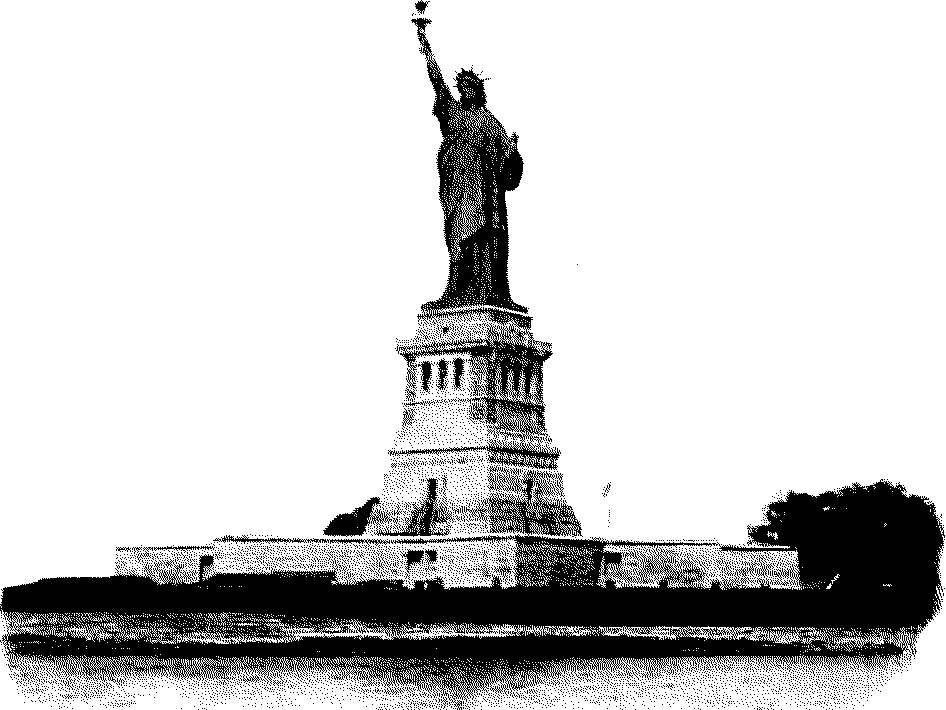
\includegraphics[width=6cm]{14_2019_Shadura1.jpg}
  %\caption{Statue of Liberty}	
  \label{fig1}
\end{figure}
\end{center}

Very soon though, during the first world war, passports returned as a temporary measure. Nothing is as permanent as temporary measures, it is often said. Passports were here to stay, and by 1947 getting rid of them has become a distant dream.

Software copyrights are in a way similar. Initially, software was not protected by copyrights or similar laws at all. In particular, in the US, prior to 1974, object code wasn't copyrightable due to lack of creativity while the consensus on the source code was that it was not copyrightable, because computer programs could be considered ideas, procedures, methods, systems, and processes.

In fact, quite a lot of software was distributed as source code: 
\begin{center}
\begin{figure}[h!]
  \centering
  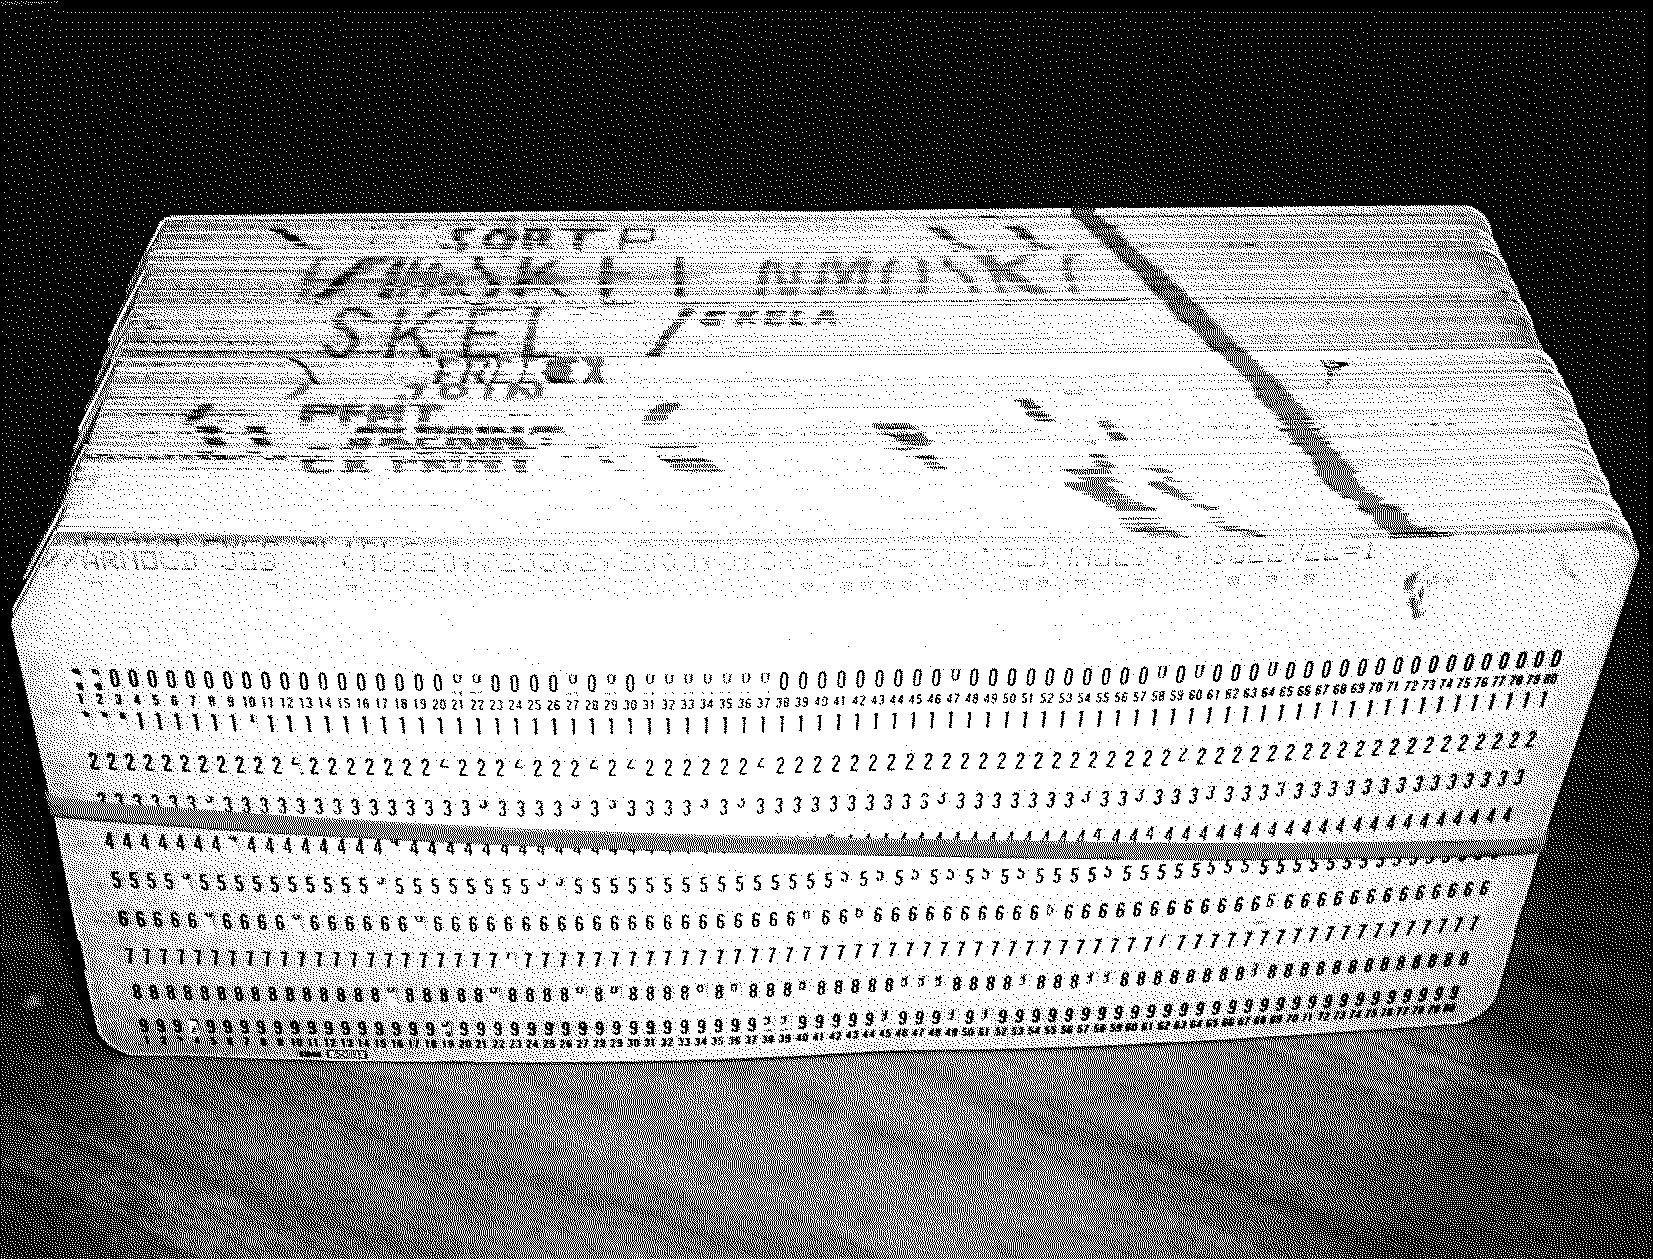
\includegraphics[width=7cm]{14_2019_Shadura2.jpg}
  
  \label{fig2}
\end{figure}
\end{center}

However, the Commission on New Technological Uses of Copyrighted Works formed in 1974, has decided that <<computer programs, to the extent that they embody an author's original creation, are proper subject matter of copyright>>. This decision followed by the US Copyright Act of 1976 giving computer programs the status of <<literary works>>.

This development has made a lot of people unhappy. One of the unhappy people was Richard Stallman. Richard Stallman was one of the people who worked at the MIT artificial intelligence lab on one of these:

\begin{center}
\begin{figure}[h!]
  \centering
  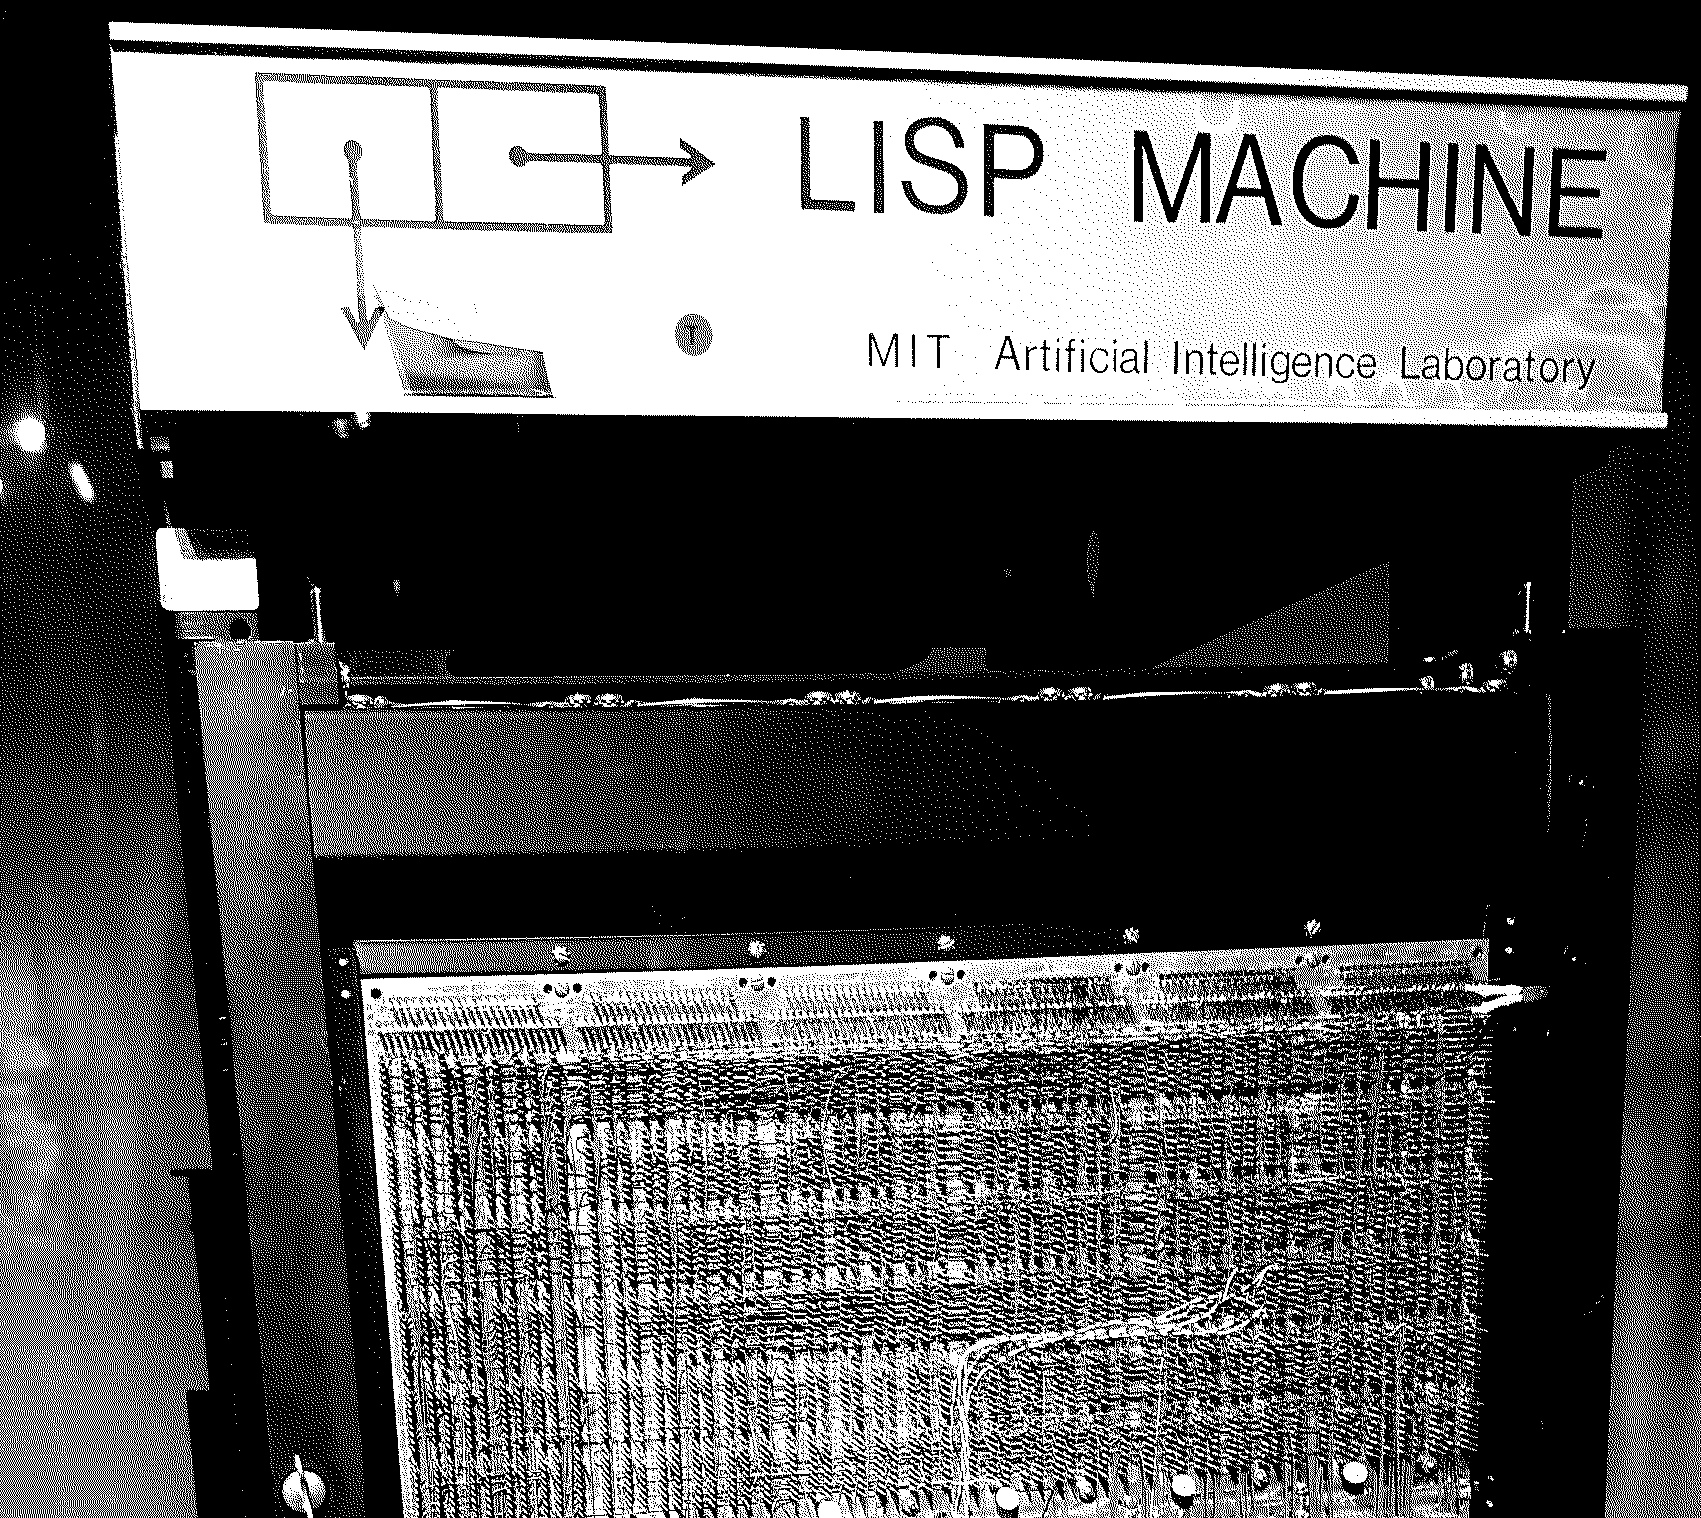
\includegraphics[width=6cm]{14_2019_Shadura3.jpg}
  
  \label{fig3}
\end{figure}
\end{center}

At MIT AI lab, there was the culture of sharing, part of the so-called hacker ethic:

\begin{quotation}
\ldots{}You would devise your own solution --- or <<hack.>> And then you'd share it with everyone else. Because\ldots{} why not?

\end{quotation}

One day, Richard Stallman was very unhappy about the new laser printer. The printer, just as the old one, was jamming paper. When this happened before, Stallman modified the printer driver to detect the jam and report it, but when he attempted to do this for the new printer, his request for the source code was rejected.

\begin{center}
\begin{figure}[h!]
  \centering
  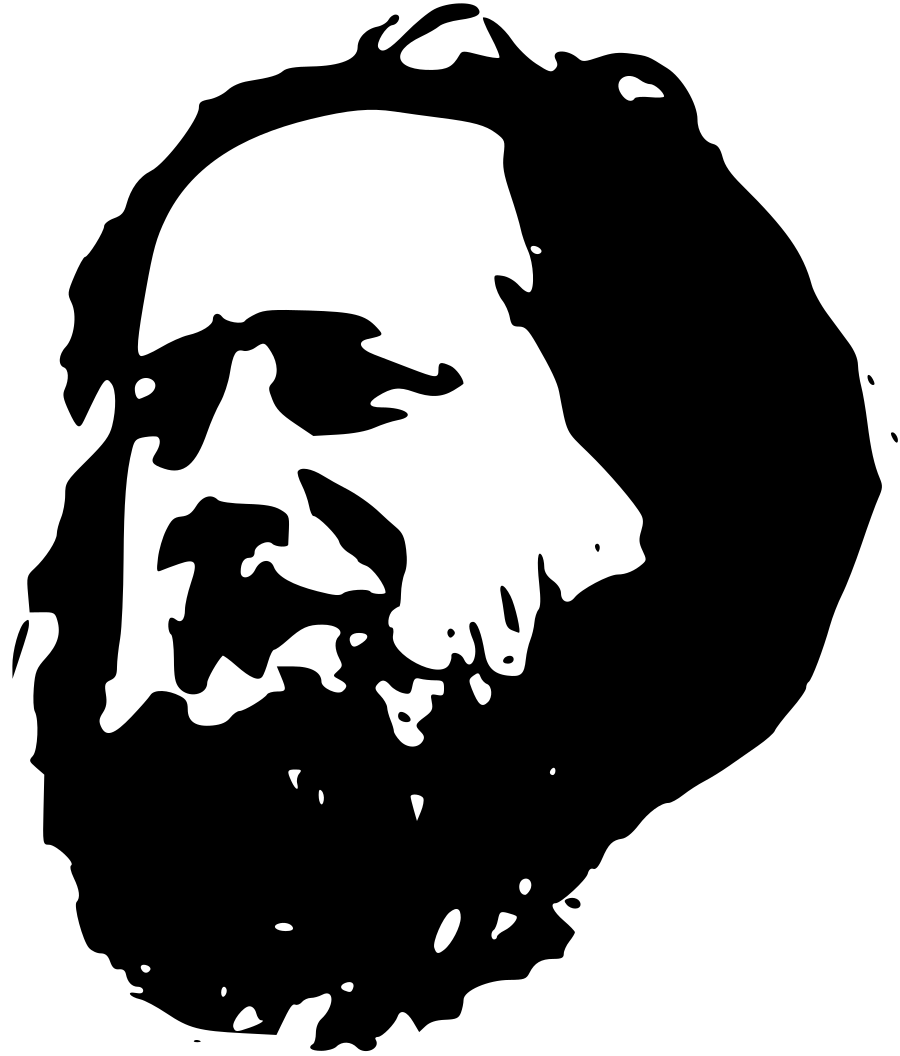
\includegraphics[width=4cm]{14_2019_Shadura4.png}
  
  \label{fig4}
\end{figure}
\end{center}

In 1983, Stallman, fed up with software coming with restrictions attached, publishes GNU Manifesto, a document which set out a plan to develop a free operating system, GNU. Several years later, he's published a detailed definition of that freedom:

\begin{enumerate}
  \item The freedom to run the program as you wish, for any purpose.
  \item The freedom to study how the program works and change it.
  \item The freedom to redistribute copies so you can help others.
  \item The freedom to distribute copies of your modified versions to others.
\end{enumerate}

Software providing those four freedoms to its users is called free software. The GNU operating system was meant to be fully free software. To protect software freedom, Stallman wrote a new license in 1989, the General Public License. This license uses the legal framework of copyright to guarantee the users can enjoy the four freedoms. It also guarantees all derivative works use the same license, and no restrictions can be added on top of the license; it explicitly makes them void.

By 1991, the GNU project completed the development of all major components of the operating system but the kernel, a core part of the operating system that manages the hardware, resources, devices\ldots{} basically, has complete control over everything in the system.

On 25 August 1991, Linus Torvalds posted the following to comp.os. minix, a newsgroup on Usenet:

\begin{quotation}
I'm doing a (free) operating system (just a hobby, won't be big and professional like gnu)

\end{quotation}

Linus has been developing the new OS  —  Linux  —  since April that year. The GNU Project soon embraced Linux, since own kernel, Hurd, was incomplete and unavailable, and another free OS, the Berkeley Software Distribution was involved in a lawsuit, and its status was unclear at the time.

In 1993, Ian Murdock announces the Debian project, which aims to build an operating system built on GNU and Linux. In Linux world, that's what a distribution is.

In many software projects, the project's creator leads the project since its inception for a long period of time. This was not the case with Debian. Instead of being a Benevolent Dictator for Life, Ian first delegated rôles to other members of the community, and then stepped down in 1996, with Bruce Perens replacing him.

\begin{quotation}
Rather than being developed by one isolated individual or group, as other distributions of Linux have been developed in the past, Debian is being developed openly in the spirit of Linux and GNU.  ---  Ian Murdock, the Debian Manifesto, 1994

\end{quotation}

What makes Debian different from other distributions? First of all, by some metrics, it's the biggest one. It supports the most different types of hardware architectures, and it has the most software packages included (if we don't count Ubuntu, which builds on top of Debian and adds software of their own). Second, it is run by a community of independent developers all around the world: there's no single company behind it, so interests of the projects can't be compromised by the interests of the company shareholders. Third, the project is built on an open democratic governance model.

\begin{quotation}

\ldots{} if you remove the community from open source software, it's just software (2003)

The Debian design process is open to ensure that the system is of the highest quality and that it reflects the needs of the user community.

\end{quotation}

Finally, the project pays a lot of attention to guarding the software freedom.

Soon after Bruce Perens became the project leader, he has proposed a document which summarised the moral principles of the Debian project, supplementing the initial \emph{Debian Manifesto} written by Murdock. The creation of the document was triggered by a discussion at Red Hat, a company behind a commercial Red Hat Linux distribution, where the idea for Red Hat to provide a set of guarantees it would always be committed to the ideals of free software was met with resistance. The document, ratified on 5 July 1997, was called the Debian Social Contact.

\begin{enumerate}
  \item Debian will remain 100\% free
  \item We will give back to the free software community
  \item We will not hide problems
  \item Our priorities are our users and free software
  \item Works that do not meet our free software standards
\end{enumerate}

DFSG:

\begin{enumerate}
  \item Free Redistribution
  \item Source Code
  \item Derived Works
  \item Integrity of The Author>>s Source Code
  \item No Discrimination Against Persons or Groups
  \item No Discrimination Against Fields of Endeavour
  \item Distribution of License
  \item License Must Not Be Specific to Debian
  \item License Must Not Contaminate Other Software
\end{enumerate}

These criteria while similar to the Four Freedoms, are more practical since they are easier to test against: it can be difficult to determine exactly how the terms of a specific license map to the user>>s freedoms. The Debian free software guidelines, on the contrary are more atomic, so it is easier to verify whether or not the license follows them. However, they define the same set of the licenses and the FSF>>s Four Freedoms.

In early 1998, a company called Netscape was about to release the source code of their browser under a free software license. A group of people, including Christine Peterson of Foresight Institute, met to discuss the promotion of free software to businesses, including Netscape.

\begin{center}
\begin{figure}[h!]
  \centering
  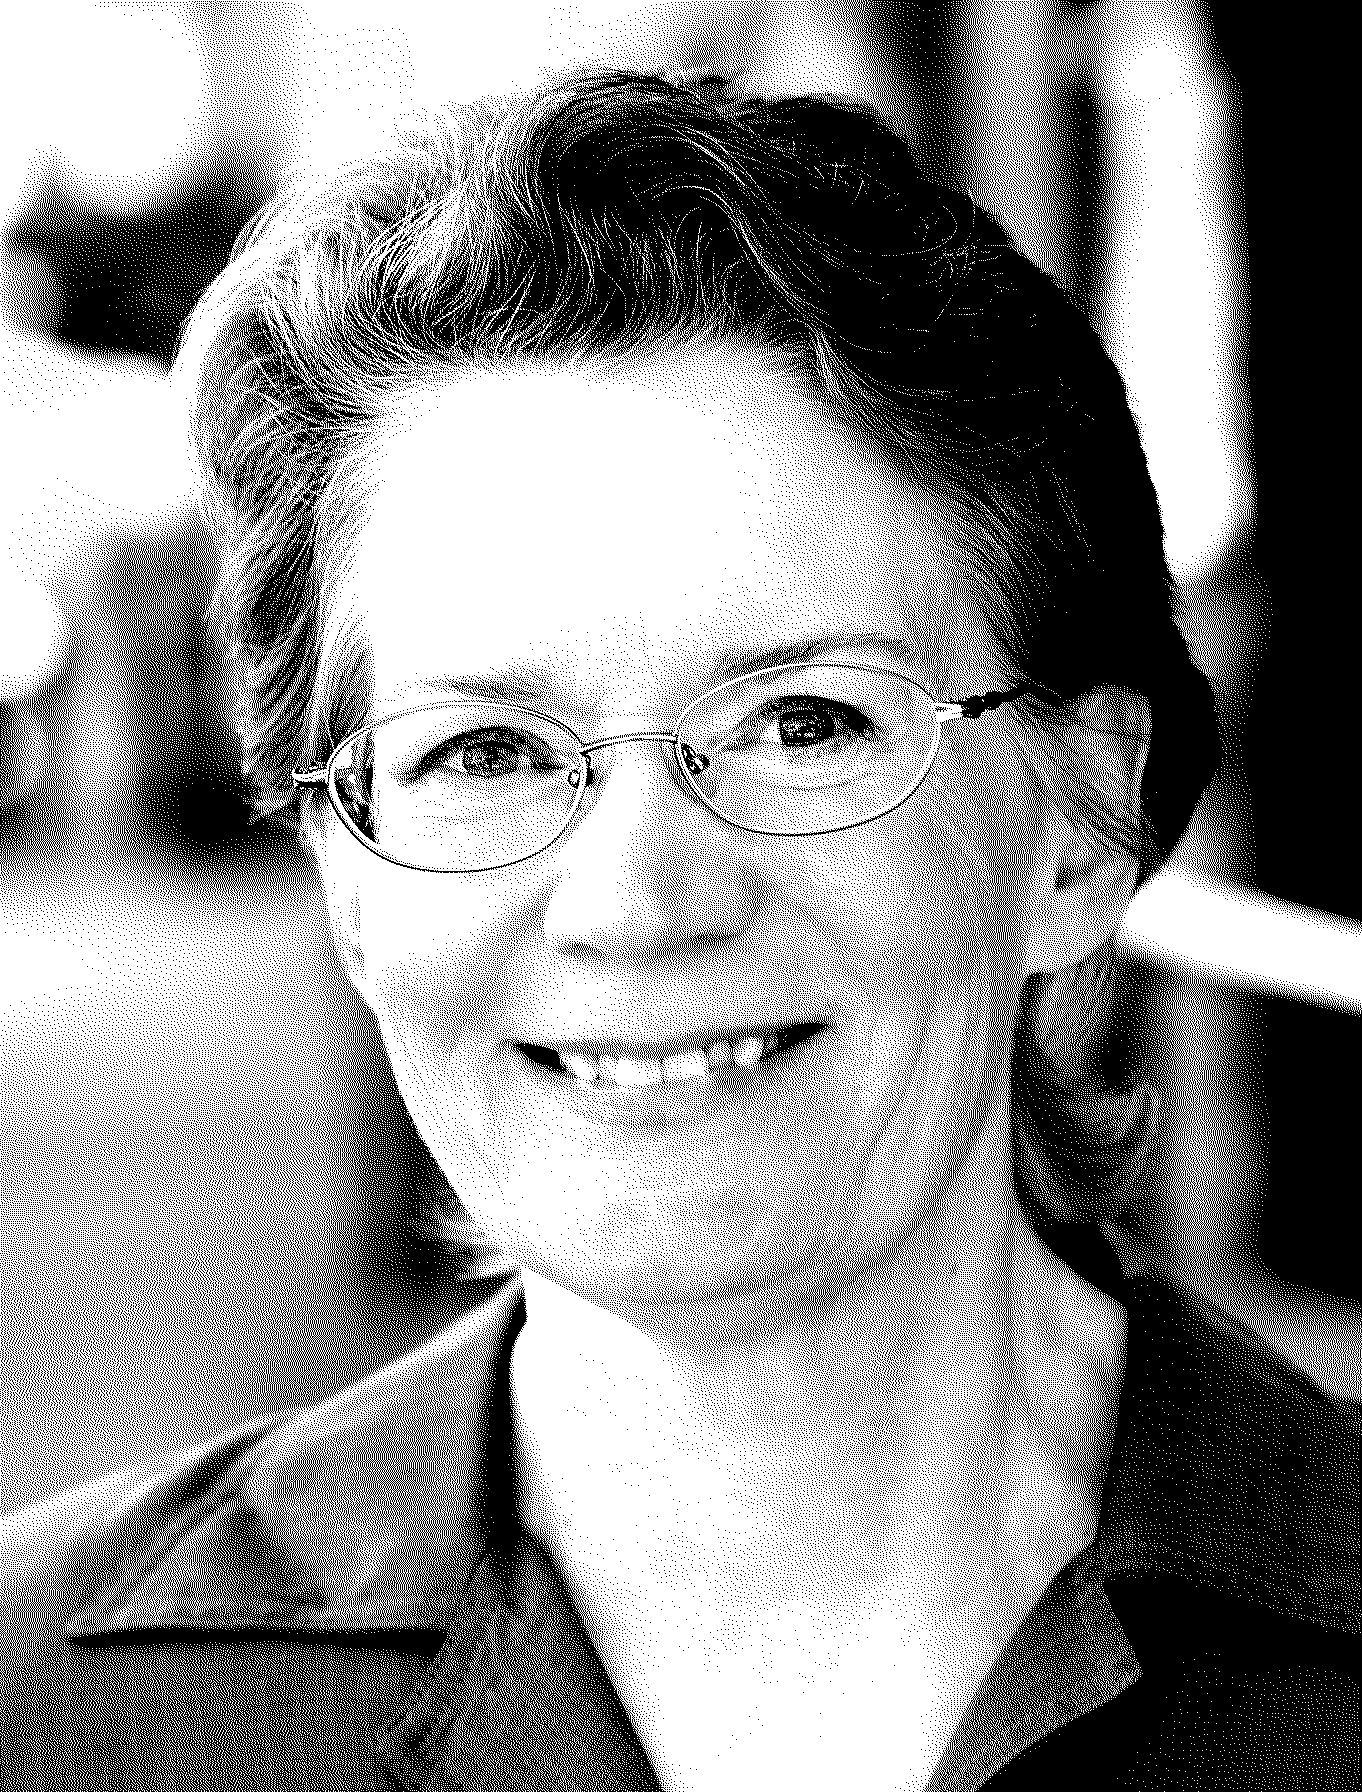
\includegraphics[width=4.5cm]{14_2019_Shadura5.jpg}
  
  \label{fig5}
\end{figure}
\end{center}

One of the topics was a new term to use because \emph{free software} was a bit confusing to people not knowing about it: they would assume it was about the price. Usually, we say \emph{We mean free as in freedom, not free as in beer}, but a new, clearer term was necessary.

During one of the meetings Christine came up with \emph{open source}, which, while not idea, seemed to her as good enough. After having discussed it with other group members, the term was eventually accepted. A new movement was started, with Bruce Perens joining the effort and establishing an organisation, the Open Source Initiative. Bruce Perens wrote a document called \emph{Open Source Definition}, based on the DFSG with references to Debian removed or replaced:

\begin{enumerate}
  \item Free Redistribution
  \item Source Code
  \item Derived Works
  \item Integrity of The Author>>s Source Code
  \item No Discrimination Against Persons or Groups
  \item No Discrimination Against Fields of Endeavour
  \item Distribution of License
  \item License Must Not Be Specific to \st{Debian} \emph{a Product}
  \item License Must Not \st{Contaminate} \emph{Restrict} Other Software
  \item \emph{License Must Be Technology-Neutral}
\end{enumerate}

Free software definition:

\begin{itemize}
  \item Promotes the philosophy of freedom
  \item Focuses on the rights of the user to use, study, modify, copy and redistribute the program for any purpose
\end{itemize}

Open source definition:

\begin{itemize}
  \item Promotes the practical values of software freedom and open development methodology
  \item Focuses on the availability of the source code and unrestricted development
\end{itemize}

Both definition require allowing commercial use.

Despite the differences, both concepts define nearly the same set of software licenses. For all practical purposes, free software and open source software mean the same thing. The main difference is in the way they define this same thing.

\begin{center}
\begin{figure}[h!]
  \centering
  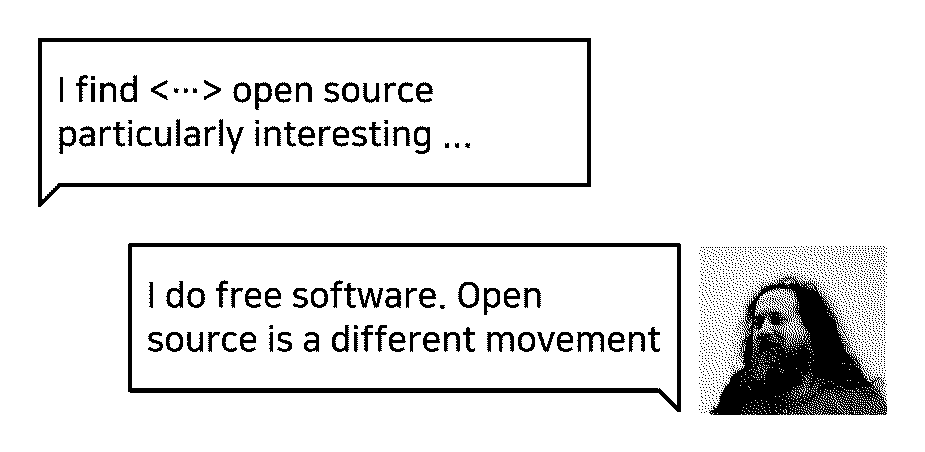
\includegraphics[width=6cm]{14_2019_Shadura6.png}
  
  \label{fig4}
\end{figure}
\end{center}


However, having initially praised open source, Richard Stallman later decided to reject it. He says the campaign for open source gets too pragmatic and doesn>>'t promote the moral principles of free software. For free software campaigners, the movement's ethical and social values are very important, and some, including Stallman, think all software should be free.

On the other hand, a lot of people love free software, but think that idea is way too radical. They accept the reality that a lot of software out there is non-free, but we can convince businesses to move to free software as much as possible. For those purposes, the concept of open source is often more useful, since it avoids telling people they're doing immoral things.

There's a concern Stallman also mentions, that both terms have ways to be misunderstood, but the \emph{wrong} meaning of open source doesn't say anything about freedom. In practice, that leads to situations, when companies promote their software calling it open source, while not providing the source code under a free software license. One of the companies which used to do that was Microsoft in 2000s, which released software under a license which basically only allowed to look at it  ---  provided you immediately forgot what you learnt from it. There more tricky situations, though.

JSON license:

\begin{itemize}
  \item The Software shall be used for Good, not Evil.
\end{itemize}

This is discrimination against fields of endeavour: you are not \linebreak allowed to do evil with this software. The author of the license, Douglas Crockford, who has also wrote JSMin, refused to change the license when was asked to. He has, however, granted <<IBM, its customers, partners, and minions>> permission <<to use JSLint for evil>>.

Do No Harm License:

\begin{quotation}
\ldots{}based on the BSD 3-clause license, but with specific exclusions for using licensed code to promote or profit from: violence, hate and division, environmental destruction, abuse of human rights, the destruction of people's physical and mental health\ldots{}

\end{quotation}

The annotated version of the open source definition states:

\begin{quotation}
We want commercial users to join our community, not feel excluded from it.

\end{quotation}


\end{document}

\documentclass[10pt, a5paper]{article}
\usepackage{pdfpages}
\usepackage{parallel}
\usepackage[T2A]{fontenc}
\usepackage{ucs}
\usepackage[utf8x]{inputenc}
\usepackage[polish,english,russian]{babel}
\usepackage{hyperref}
\usepackage{rotating}
\usepackage[inner=2cm,top=1.8cm,outer=2cm,bottom=2.3cm,nohead]{geometry}
\usepackage{listings}
\usepackage{graphicx}
\usepackage{wrapfig}
\usepackage{longtable}
\usepackage{indentfirst}
\usepackage{array}
\newcolumntype{P}[1]{>{\raggedright\arraybackslash}p{#1}}
\frenchspacing
\usepackage{fixltx2e} %text sub- and superscripts
\usepackage{icomma} % коскі ў матэматычным рэжыме
\PreloadUnicodePage{4}

\newcommand{\longpage}{\enlargethispage{\baselineskip}}
\newcommand{\shortpage}{\enlargethispage{-\baselineskip}}

\def\switchlang#1{\expandafter\csname switchlang#1\endcsname}
\def\switchlangbe{
\let\saverefname=\refname%
\def\refname{Літаратура}%
\def\figurename{Іл.}%
}
\def\switchlangen{
\let\saverefname=\refname%
\def\refname{References}%
\def\figurename{Fig.}%
}
\def\switchlangru{
\let\saverefname=\refname%
\let\savefigurename=\figurename%
\def\refname{Литература}%
\def\figurename{Рис.}%
}

\hyphenation{admi-ni-stra-tive}
\hyphenation{ex-pe-ri-ence}
\hyphenation{fle-xi-bi-li-ty}
\hyphenation{Py-thon}
\hyphenation{ma-the-ma-ti-cal}
\hyphenation{re-ported}
\hyphenation{imp-le-menta-tions}
\hyphenation{pro-vides}
\hyphenation{en-gi-neering}
\hyphenation{com-pa-ti-bi-li-ty}
\hyphenation{im-pos-sible}
\hyphenation{desk-top}
\hyphenation{elec-tro-nic}
\hyphenation{com-pa-ny}
\hyphenation{de-ve-lop-ment}
\hyphenation{de-ve-loping}
\hyphenation{de-ve-lop}
\hyphenation{da-ta-ba-se}
\hyphenation{plat-forms}
\hyphenation{or-ga-ni-za-tion}
\hyphenation{pro-gramming}
\hyphenation{in-stru-ments}
\hyphenation{Li-nux}
\hyphenation{sour-ce}
\hyphenation{en-vi-ron-ment}
\hyphenation{Te-le-pathy}
\hyphenation{Li-nux-ov-ka}
\hyphenation{Open-BSD}
\hyphenation{Free-BSD}
\hyphenation{men-ti-on-ed}
\hyphenation{app-li-ca-tion}

\def\progref!#1!{\texttt{#1}}
\renewcommand{\arraystretch}{2} %Іначай формулы ў матрыцы зліпаюцца з лініямі
\usepackage{array}

\def\interview #1 (#2), #3, #4, #5\par{

\section[#1, #3, #4]{#1 -- #3, #4}
\def\qname{LVEE}
\def\aname{#1}
\def\q ##1\par{{\noindent \bf \qname: ##1 }\par}
\def\a{{\noindent \bf \aname: } \def\qname{L}\def\aname{#2}}
}

\def\interview* #1 (#2), #3, #4, #5\par{

\section*{#1\\{\small\rm #3, #4. #5}}

\def\qname{LVEE}
\def\aname{#1}
\def\q ##1\par{{\noindent \bf \qname: ##1 }\par}
\def\a{{\noindent \bf \aname: } \def\qname{L}\def\aname{#2}}
}

\switchlang{en}
\begin{document}
\title{Wafer conference management system}
\author{Andrej Shadura, Bratislava, Slovakia\footnote{\url{andrew@shadura.me}, \url {https://lvee.org/ru/abstracts/319}}}
\maketitle
\begin{abstract}
Wafer is a web based conference management software based on Python and Django, targeted at small (or medium) sized conferences, licensed under the ISC License, and developed at GitHub. The most known conference using Wafer is DebConf, which switched to it from the old and poorly supported Pentabarf system.
\end{abstract}
Main features of wafer are the website content management, talks submission system and the talks review process, and the conference schedule management.

\subsection*{Web Contents}

Static information for the conference is represented with \emph{pages}, which contain Markdown-formatted contents, and images uploaded as \emph{files}. To provide hierarchical organisation, so-called \emph{container pages} are used: they are parent objects for other pages, and provide minimal content, if any. Pages are stored in the database, and can be edited through the web UI. An alternative is to store them Markdown files (e.g. in a Git repo) with a YAML-formatted preamble and load them into the database with a special management command.

Wafer includes a simple system to generate single levels menus (either static or dynamic ones) for the navigation bar at the top of each page. By default, only two kinds of menu items are dynamically generated: \emph{pages} and \emph{sponsors} menus, and menu items.

Page menus appear when a page is marked for inclusion in the navigation menu.

The sponsor menu is a single sub-menu listing the sponsors in order of precedence with links to their sponsor pages. It also includes links to the full list of sponsors and the list of sponsorship packages at the bottom of the sub-menu.

\emph{Sponsor packages} describe the details of the various sponsorship variants, including the order in which the list on the sponsor packages page is composed. The details about the sponsors (a description) can be formatted using Markdown and uploaded images as with the rest of pages.

The default sponsor template expect each sponsor to have an image for the main logo to be used in the sponsor list (uploaded files can be associated with a sponsor and a name in the admin interface). Also there is an example template block for adding sponsors as a footer to all pages (which can contain its own associated image, e.g. a different size one).

\subsubsection*{Talks}

Users can submit talks from their profile page. The abstract can be formatted using markdown-formatted. Talks have following publicly visible fields: \emph{title}, an \_abstract \_(which can be markdown-formatted) and \emph{authors}. Two additional private fields are \_notes \_(written by the author, e.g. special equipment requirements, etc.) and \_private notes \_(visible to organisers only, e.g. assigned reviewers, etc.).

There also also user-defined \emph{talk types}, which need to be specifed before opening up talk submissions, e.g. \emph{Tutorial}, \emph{Short Talks}, etc. Each \verb@Talk Type@ can be open or closed for submissions individually via the admin interface.

Users can submit talks from their profile page using the \emph{Submit Talk Proposal} option. Talks can have multiple authors, but only one of them is the \emph{corresponding author} who can edit the talk submission.

The talk lifecycle can include the following states:

\begin{itemize}
  \item Submitted (the initial state),
  \item Under Consideration (after at least one review was left),
  \item Withdrawn (talk was withdrawn by the talk submitter before decision was made),
  \item Provisionally Accepted (positive decision on conferences with \linebreak mandatory submitter's confirmation),
  \item Accepted (positive decision),
  \item Cancelled (talk was withdrawn by the talk submitter after the positive decision),
  \item Not Accepted (negative decision).
\end{itemize}

Multiple talk tracks are supported as an option; if this feature is turned on, submitters have to additionally choose a track for each submission.

\subsection*{Talks review process}

The \emph{Talk Reviewers} group members have permission to view all talk submissions (not only accepted ones), including notes and private notes, and are able to leave reviews on talks.

The \emph{Talk Mentors} group members have the same list of permissions and additionally are able to edit submitted talks, and view and edit both notes and private notes.

Talk Mentors can review Talks are reviewed by user-defined \emph{metrics}.

Talk Reviewers see a \emph{Review} button on talk pages, and will be prompted to review each talk by each metric. The reviewer has to put a numerical score for each metric and can also leave a textual review. If a reviewer re-reviews a talk, the previous review is updated.

Talks are shown in the publicly available talk listing, where reviewers will see additional items and special emblems (e.g. a clock symbol if the submission was changed making their review out of date).

\subsection*{Schedule}

Wafer scheduling concept is based on days, venues, slots, and items.

Each \emph{venue} is associated with a number of \emph{days} of the conference. Each \emph{slot} is assigned to a given day, and has a start and end time (fixed or based on the end time of a previous slot in a sequence).

Each \emph{item} in the schedule has a number of slots, a venue and either a talk or a page. Each talk can only be assigned to a single schedule item, but pages can be assigned to multiple schedule items (this simplifies scheduling such service items as tea breaks).


\begin{thebibliography}{9}
\bibitem{bib1} I. Olea. An improvised list of opensource conference management software \url{http://olea.org/diario/2017/10/27/opensource-conference-management-software.html}
\bibitem{bib2} CTPUG/wafer: A wafer-thin web application for running small conferences. Built using Django \url{http://github.com/CTPUG/wafer}
\bibitem{bib3} Wafer 0.7.6a documentation \url{https://wafer.readthedocs.io/en/latest/}
\end{thebibliography}
\end{document}

\documentclass[10pt, a5paper]{article}
\usepackage{pdfpages}
\usepackage{parallel}
\usepackage[T2A]{fontenc}
\usepackage{ucs}
\usepackage[utf8x]{inputenc}
\usepackage[polish,english,russian]{babel}
\usepackage{hyperref}
\usepackage{rotating}
\usepackage[inner=2cm,top=1.8cm,outer=2cm,bottom=2.3cm,nohead]{geometry}
\usepackage{listings}
\usepackage{graphicx}
\usepackage{wrapfig}
\usepackage{longtable}
\usepackage{indentfirst}
\usepackage{array}
\newcolumntype{P}[1]{>{\raggedright\arraybackslash}p{#1}}
\frenchspacing
\usepackage{fixltx2e} %text sub- and superscripts
\usepackage{icomma} % коскі ў матэматычным рэжыме
\PreloadUnicodePage{4}

\newcommand{\longpage}{\enlargethispage{\baselineskip}}
\newcommand{\shortpage}{\enlargethispage{-\baselineskip}}

\def\switchlang#1{\expandafter\csname switchlang#1\endcsname}
\def\switchlangbe{
\let\saverefname=\refname%
\def\refname{Літаратура}%
\def\figurename{Іл.}%
}
\def\switchlangen{
\let\saverefname=\refname%
\def\refname{References}%
\def\figurename{Fig.}%
}
\def\switchlangru{
\let\saverefname=\refname%
\let\savefigurename=\figurename%
\def\refname{Литература}%
\def\figurename{Рис.}%
}

\hyphenation{admi-ni-stra-tive}
\hyphenation{ex-pe-ri-ence}
\hyphenation{fle-xi-bi-li-ty}
\hyphenation{Py-thon}
\hyphenation{ma-the-ma-ti-cal}
\hyphenation{re-ported}
\hyphenation{imp-le-menta-tions}
\hyphenation{pro-vides}
\hyphenation{en-gi-neering}
\hyphenation{com-pa-ti-bi-li-ty}
\hyphenation{im-pos-sible}
\hyphenation{desk-top}
\hyphenation{elec-tro-nic}
\hyphenation{com-pa-ny}
\hyphenation{de-ve-lop-ment}
\hyphenation{de-ve-loping}
\hyphenation{de-ve-lop}
\hyphenation{da-ta-ba-se}
\hyphenation{plat-forms}
\hyphenation{or-ga-ni-za-tion}
\hyphenation{pro-gramming}
\hyphenation{in-stru-ments}
\hyphenation{Li-nux}
\hyphenation{sour-ce}
\hyphenation{en-vi-ron-ment}
\hyphenation{Te-le-pathy}
\hyphenation{Li-nux-ov-ka}
\hyphenation{Open-BSD}
\hyphenation{Free-BSD}
\hyphenation{men-ti-on-ed}
\hyphenation{app-li-ca-tion}

\def\progref!#1!{\texttt{#1}}
\renewcommand{\arraystretch}{2} %Іначай формулы ў матрыцы зліпаюцца з лініямі
\usepackage{array}

\def\interview #1 (#2), #3, #4, #5\par{

\section[#1, #3, #4]{#1 -- #3, #4}
\def\qname{LVEE}
\def\aname{#1}
\def\q ##1\par{{\noindent \bf \qname: ##1 }\par}
\def\a{{\noindent \bf \aname: } \def\qname{L}\def\aname{#2}}
}

\def\interview* #1 (#2), #3, #4, #5\par{

\section*{#1\\{\small\rm #3, #4. #5}}

\def\qname{LVEE}
\def\aname{#1}
\def\q ##1\par{{\noindent \bf \qname: ##1 }\par}
\def\a{{\noindent \bf \aname: } \def\qname{L}\def\aname{#2}}
}

\switchlang{ru}
\begin{document}
\title{Опыт преподавания языка Ruby в рамках дисциплины <<Cовременные технологии разработки программного обеспечения>>}
\author{Максим Стержанов, Минск, Belarus\footnote{\url{msterjanov@gmail.com}, \url {https://lvee.org/ru/abstracts/320}}}
\maketitle
\begin{abstract}
Experience of teaching master degree students Ruby/RoR is detailed. We explain basic course structure, list main difficulties students face and way to resolve them. 
\end{abstract}
Кафедра Информатики БГУИР ведет подготовку бакалавров и магистров по специальности <<Информатика и технологии программирования>>. Одной из основных специальных дисциплин, читаемых при подготовке магистрантов является <<Современные технологии разработки программного обеспечения>>(СТРПО). Целью преподавания данной дисциплины является предоставление обучаемым знаний и умений в области проектирования, разработки, тестирования, отладки и внедрения программного обеспечения (ПО) вычислительной техники с использованием современных технологий.

В данной работе описывается перечень лабораторных задач,\linebreak предлагаемых студентам  для проработки и закрепления материала по предмету СТРПО в 2017 /2018 учебном году.

Устный опрос показывает, что основную группу магистрантов составляют программисты-практики с профильным высшим образованием (БГУИР или БГУ) и опытом работы в софтверных компаниях от 2 до 4 лет. Следовательно, данная аудитория должна иметь глубокое понимание теоретических основ информатики, опыт практического использования одного или нескольких языков и технологий. Исходя из этого, образовательный процесс фокусировался на ключевых особенностях языка Ruby.

В рамках первой лабораторной работы магистрантам предлагается познакомиться с основами написания скриптов на динамическом объектно-ориентированном языке Ruby и проработать применение базовых конструкций языка. В качестве среды разработки предлагается тестовый редактор Sublime Text или специализированная среда RubyMine. В рамках данной работы предлагается реализация простейшего алгоритма шифрования.

Вторая лабораторная работа посвящена изучению функционального стиля программирования в Ruby. Все функции в Ruby являются методами, то есть свойственны объектам. Цель выполнения работы --- изучение итераторов, блоков и замыканий. Также магистратам предлагается провести сравнительный анализ объектов, которые можно вызывать (proc, lambda, method).

В рамках третьей лабораторной работы магистрантам предлагается применить на практике знания об объектной модели Ruby. Мы предполагаем, что большая часть аудитории знакома с понятиями ООП на примере других языков. Ruby является полностью объектно-ориентированным языком: числа, строки, регулярные выражения, массивы --- это все объекты определенных классов.  Магистрантам предлагается изучить концепцию модуля и примеси, инкапсуляцию. Результатом выполнения работы является реализация взаимодействия объектов в соответствии с индивидуальным заданием.

Четвертая и пятая лабораторная работы посвящены метапрограммированию в объектной модели Ruby. Под метапрограммированием понимается расширение и изменение абстракций языка \cite{bib1}. Магистранты изучают способы динамического определения и вызова методов, применение method\_missing, синглетон-методы, синг\-летон-классы, отрабатывают техники динамического изменения \linebreak классов и методов.

На шестой, заключительной работе, магистрантам предлагается обобщить полученные знания при построении серверной части веб-приложения на платформе Ruby on Rails. Rails представляет собой среду, облегчающую разработку, развертывание и обслуживание веб-приложений \cite{bib3}. Магистранты создают REST ориентированные сервисы в соответствии с предложенными вариантами заданий (библиотека, ресторан, больница и т.д.). Задачей является продемонстрировать умение пользоваться фреймворком объектно-реляционного отображения ActiveRecord и основами ресурсного роутинга Rails. Реализация клиентской части (HTML представления) не требуется. Тестирование осуществляется при помощи программы POSTMAN (либо аналогичной).

Содержание лабораторных работ построено в единой логике и позволяет эффективно обучить магистрантов приемам программирования на современном скриптовом языке Ruby.

Опыт преподавания языка Ruby для магистрантов выявил некоторые проблемы:

\begin{itemize}
  \item недостаточная подготовка в области программирования (отсутствие умений и навыков разработки, отсутствие понятийного аппарата ООП) после окончания ВУЗа;
  \item нехватка времени для самостоятельной работы в связи с загруженностью по основному месту работы;
  \item выполнение работ на поверхностном уровне, нежелание переучиваться и погружаться в детали  новой и незнакомой технологии.
\end{itemize}

Для решения данных проблем отстающим магистрантам были предложены упрощенные версии индивидуальных заданий.

Не смотря на указанные сложности, изучение языка Ruby и платформы Ruby on Rails дает магистрантам уникальные возможности для расширения собственного багажа знаний и  опыта, которыми нельзя не воспользоваться.



\begin{thebibliography}{9}
\bibitem{bib1} A. Hunt. Programming Ruby./ A. Hunt, D. Thomas --- М.: Финансы и статистика, 2004. --- 864 p.
\bibitem{bib2} Perrotta P. Metaprogramming Ruby 2: Program Like the Ruby Pros. -- The Pragmatic Programmers, 2004. --- 262 p.
\bibitem{bib3} Руби С. Rails 4. Гибкая разработка веб-приложений. С. Руби, Д. Томас, Д. Хэнссон --- СПб.: Питер, 2014. --- 448 с.
\end{thebibliography}
\end{document}

\documentclass[10pt, a5paper]{article}
\usepackage{pdfpages}
\usepackage{parallel}
\usepackage[T2A]{fontenc}
\usepackage{ucs}
\usepackage[utf8x]{inputenc}
\usepackage[polish,english,russian]{babel}
\usepackage{hyperref}
\usepackage{rotating}
\usepackage[inner=2cm,top=1.8cm,outer=2cm,bottom=2.3cm,nohead]{geometry}
\usepackage{listings}
\usepackage{graphicx}
\usepackage{wrapfig}
\usepackage{longtable}
\usepackage{indentfirst}
\usepackage{array}
\newcolumntype{P}[1]{>{\raggedright\arraybackslash}p{#1}}
\frenchspacing
\usepackage{fixltx2e} %text sub- and superscripts
\usepackage{icomma} % коскі ў матэматычным рэжыме
\PreloadUnicodePage{4}

\newcommand{\longpage}{\enlargethispage{\baselineskip}}
\newcommand{\shortpage}{\enlargethispage{-\baselineskip}}

\def\switchlang#1{\expandafter\csname switchlang#1\endcsname}
\def\switchlangbe{
\let\saverefname=\refname%
\def\refname{Літаратура}%
\def\figurename{Іл.}%
}
\def\switchlangen{
\let\saverefname=\refname%
\def\refname{References}%
\def\figurename{Fig.}%
}
\def\switchlangru{
\let\saverefname=\refname%
\let\savefigurename=\figurename%
\def\refname{Литература}%
\def\figurename{Рис.}%
}

\hyphenation{admi-ni-stra-tive}
\hyphenation{ex-pe-ri-ence}
\hyphenation{fle-xi-bi-li-ty}
\hyphenation{Py-thon}
\hyphenation{ma-the-ma-ti-cal}
\hyphenation{re-ported}
\hyphenation{imp-le-menta-tions}
\hyphenation{pro-vides}
\hyphenation{en-gi-neering}
\hyphenation{com-pa-ti-bi-li-ty}
\hyphenation{im-pos-sible}
\hyphenation{desk-top}
\hyphenation{elec-tro-nic}
\hyphenation{com-pa-ny}
\hyphenation{de-ve-lop-ment}
\hyphenation{de-ve-loping}
\hyphenation{de-ve-lop}
\hyphenation{da-ta-ba-se}
\hyphenation{plat-forms}
\hyphenation{or-ga-ni-za-tion}
\hyphenation{pro-gramming}
\hyphenation{in-stru-ments}
\hyphenation{Li-nux}
\hyphenation{sour-ce}
\hyphenation{en-vi-ron-ment}
\hyphenation{Te-le-pathy}
\hyphenation{Li-nux-ov-ka}
\hyphenation{Open-BSD}
\hyphenation{Free-BSD}
\hyphenation{men-ti-on-ed}
\hyphenation{app-li-ca-tion}

\def\progref!#1!{\texttt{#1}}
\renewcommand{\arraystretch}{2} %Іначай формулы ў матрыцы зліпаюцца з лініямі
\usepackage{array}

\def\interview #1 (#2), #3, #4, #5\par{

\section[#1, #3, #4]{#1 -- #3, #4}
\def\qname{LVEE}
\def\aname{#1}
\def\q ##1\par{{\noindent \bf \qname: ##1 }\par}
\def\a{{\noindent \bf \aname: } \def\qname{L}\def\aname{#2}}
}

\def\interview* #1 (#2), #3, #4, #5\par{

\section*{#1\\{\small\rm #3, #4. #5}}

\def\qname{LVEE}
\def\aname{#1}
\def\q ##1\par{{\noindent \bf \qname: ##1 }\par}
\def\a{{\noindent \bf \aname: } \def\qname{L}\def\aname{#2}}
}

\switchlang{ru}
\begin{document}
\title{Применение аппарата конечных автоматов}
\author{Чеусов Алексей, Минск, Беларусь \footnote{\url{vle@gmx.net}, \url {https://lvee.org/ru/abstracts/308}}}

\begin{document}
\maketitle
\begin{abstract}
In this presentation we define the finite state automata (FSA), Moore and Mealy machines, and Finite State Transducers. We\-ighted and stochastic finite state machines are described. Also, a few well-known and custom algorithms based on finite state machines, are described.
\end{abstract}

Аппарат конечных автоматов -- один из базовых и наиболее важных
понятий в информатике и программировании.  Конечные автоматы изучаются
во всех без исключения университетах и институтах по специальностям,
так или иначе связанным с информатикой и программированием. Тем не
менее, по моему мнению недостаточное внимание в нашей системе
образования уделяется практическому их применению, что, на моей
взгляд, негативно сказывается на уровне подготовке отечественных
программистов. Данным докладом хотелось бы хотя бы частично
ликвидировать это досадную ситцацию, и пробудить интерес к во
многом забытым конечным автоматам. С этой целью будут приведены 
примеры практических задач, реашемых с их помощью.

Прежде всего хочется сказать, что данная статья является дополнением
к презентации, доступной на сайте \url{http://lvee.org} \linebreak или по ссылке ~
\href{http://www.mova.org/~cheusov/pub/lvee/2019/fsa\_presentation.pdf}{http://www.mova.org/\textasciitilde\,cheusov/pub/lvee/2019/fsa\_presentation.pdf}. 

Начать следует с определений и теорем, хорошо знакомых любому
выпускнику ВУЗ-а по технической специальности.

\textbf{Определение:} Недетерминированным конечным автоматом \linebreak (НКА) называется пятерка
\mbox{$<I,S,Q,F,\delta>$}, где
\begin{itemize}
\item $I$ -- конечное непустое множество символов (алфавит);
\item $S$ -- конечное непустое множество состояний;
\item $Q$ -- множество стартовых состояний, $Q \subseteq S$;
\item $F$ -- множество конечных состояний, $F \subseteq S$;
\item $\delta$ -- отношение переходов $\delta \subseteq S \times I \times S$
  (или, иначе, $\delta: S \times I \rightarrow 2^S$).
\end{itemize}

Языком КА является множество различных последовательностей символов алфавита, допускаемых
конечным автоматом, т.е., цепочек символов вдоль пути от стартового до конечного состояния КА.

\textbf{Определение:} Регулярный язык над алфавитом $\Sigma$ определяется следующим образом:
\begin{itemize}
\item Пустой язык $\emptyset$ и язык $\{\epsilon\}$, состоящий из пустой строки, является регулярным языком;
\item $\{a\}$, где $a \in \Sigma$, является регулярным языком;
\item Если $A$ и $B$ регулярные языки, то $A \cup B$ (объединение), $A \bullet B$ (конкатенация),
  и $A\ast$ (звезда Клини) являются регулярными языками;
\item Никакие другие языки над $\Sigma$ не являются регулярными.
\end{itemize}
Этот формализм дает нам так называемые <<регулярные выражения>>.

\textbf{Определение:} Детерминированным конечным автоматом \linebreak (ДКА) является пятерка $<I,S,q,F,\delta>$, где
\begin{itemize}
\item $I$ -- конечное непустое множество символов (алфавит);
\item $S$ -- конечное непустое множество состояний;
\item $q$ -- стартовое состояние, $q \in S$.
\item $F$ -- множество конечных состояний, $F \subseteq S$.
\item $\delta$ -- функция переходов: $\delta: S \times I \rightarrow S$
\end{itemize}

\textbf{Теоремы}:
\begin{itemize}
\item НКА и ДКА -- эквивалентные формализмы, т.е., для каждого НКА
  существует эквивалентный ему ДКА, обратное верно по определению.
\item В общем случае ДКА может быть экспоненциально больше (по
  количеству состояний) по сравнению с эквивалентным ему НКА.
\item Для любого ДКА существует только один (с точностью до изоморфизма) минимальный ДКА,
  эквивалентный ему.
\item Регулярные языки и конечные автоматы -- эквивалентные
  формализмы, то есть, для любого КА существует эквивалентный ему
  регулярный язык и наоборот.
\item Конечные автоматы замкнуты относительно операций объединения, вычитания, пересечения, дополнения
  и звезды Клини.
\end{itemize}

\textbf{Алгоритм} построения ДКА из НКА представлен ниже.

~

~

\begin{algorithm}[h!]
  \DontPrintSemicolon
  \SetKwInOut{Input}{input}
  \SetKwInOut{Output}{output}
  \Input{NFA = $<I,S,Q,F,\delta>$}
  \Output{DFA = $<I,S^{\prime},q^\prime,F^{\prime},\delta^{\prime}>$}
  \SetAlgoLined
%  \SetAlgoNoEnd
  $\delta^\prime := \emptyset, q^\prime := \{s | s \in Q\}, S^\prime := \{q^\prime\}$\;
  $seen := \{q^\prime\}, queue := [q^\prime]$\;
  \While{$queue \neq \emptyset$}{
    $src\_states \leftarrow queue$\;
    \For{$i \in I$}{
      $trg\_states := \{s^{trg} | (s^{src},i,s^{trg}) \in \delta, s^{src} \in src\_states\}$\;
      \If{$trg\_states \neq \emptyset$}{
        $\delta^\prime \leftarrow (src\_states, i, trg\_states)$\;
        $S^\prime \leftarrow trg\_states$\;
        \If{$trg\_states \notin seen$}{
          $queue \leftarrow trg\_states$\;
          $seen \leftarrow trg\_states$\;
        }
      }
    }
  }
  $F^\prime := \{state\_set \in S^\prime | \exists s \in state\_set, s \in F\}$
  \caption{nfa2dfa algorithm AKA <<Subset construction>>}
\end{algorithm}

Введем два дополнительных оператора:
\begin{itemize}
\item R -- оператор инвертирования. $L(R(KA)) = \{inverse(w) | w \in L(KA)\}$
\item D -- оператор построения ДКА по НКА.
\end{itemize}

\textbf{Алгоритм} Бжозовского построения минимального ДКА по \linebreak НКА:\\
$MinDFA = (D \circ R \circ D \circ R) KA$

\textbf{Замечание:} В отличие от большинства других алгоритмов построения минимального ДКА, алгоритм
Бжозовского строит минимальный ДКА по НКА!

\newpage
Алгоритм проверки, входит ли строка в язык ДКА.

\begin{algorithm}[h!]
  \DontPrintSemicolon
  \SetKwInOut{Input}{input}
  \SetKwInOut{Output}{output}
  \Input{DFA = $<I,S,q,F,\delta>, Text=[t_1, t_2 \dots t_n], t_i \in I$}
  \Output{$true$ \textbf{or} $false$}
  \SetAlgoLined
  %    \SetAlgoNoEnd
  $state := q$\;
  \For{$i$ from $1$ to $n$}{
    \uIf{$\delta$ is defined on $(state, t_i)$}{
      $state := \delta(state, t_i)$\;
    }\Else{
      \textbf{return} false\;
    }
  }
  \textbf{return} $(state \in F)$\;
  \caption{Сопоставление строки с ДКА. Сложность алгоритма: $O(n)$}
\end{algorithm}

Алгоритм проверки, входит ли строка в язык НКА.
\begin{algorithm}
  \DontPrintSemicolon
  \SetAlgoLined
  \SetKwInOut{Input}{input}
  \SetKwInOut{Output}{output}
  \Input{NFA = $<I,S,Q,F,\delta>, Text=[t_1, t_2 \dots t_n], t_i \in I$}
  \Output{$true$ \textbf{or} $false$}
  $states := Q$\;
  \For{$i$ from $1$ to $n$ \textbf{and} $states \neq \emptyset$}{
    $states := \{trg | (src, t_i, trg) \in \delta, src \in states\}$\;
  }
  \textbf{return} $(\exists s \in states, s \in F)$\;
  \caption{Сопоставление строки с НКА. Сложность алгоритма: $O(n * |S|)$}
\end{algorithm}

\textbf{Определение:}
Автомат Мура -- это шестерка $<I,O,S,q,\delta, \lambda>$, где
\begin{itemize}
\item $I$ -- входной алфавит, конечное непустое множество входных символов;
\item $O$ -- выходной алфавит, конечное непустое множество выходных символов;
\item $S$ -- конечное непустое множество состояний;
\item $q$ -- стартовое состояние, $q \in S$;
\item $\delta$ -- функция переходов $\delta: S \times I \rightarrow S$;
\item $\lambda$ -- функция выходов $\lambda: S \rightarrow O$.
\end{itemize}

\textbf{Определение:}
Автомат Мили -- это шестерка $<I,O,S,q,\delta, \lambda>$.
\begin{itemize}
\item $I$ -- входной алфавит, конечное непустое множество входных символов;
\item $O$ -- выходной алфавит, конечное непустое множество выходных символов;
\item $S$ -- конечное непустое множество состояний;
\item $q$ -- стартовое состояние, $q \in S$;
\item $\delta$ -- функция переходов $\delta: S \times I \rightarrow S$
\item $\lambda$ -- функция выходов $\lambda: S \times I \rightarrow O$
\end{itemize}
\textbf{Note:} На практике мы часто работаем с \textit{частично определенными} ДКА, НКА,
автоматами Мура и Мили, т.е., автоматами с частично определенной функцией переходов.

\textbf{Теорема:} Автоматы Мура и Мили -- эквивалентные формализмы.

\textbf{Определение:} 
Взвешенный конечный автомат -- это шестерка $<I,S,Q,F,\delta, \omega>$.
\begin{itemize}
\item $I$ -- конечное непустое множество символов (алфавит);
\item $S$ -- конечное непустое множество состояний;
\item $Q$ -- множество стартовых состояний, $Q \subseteq S$;
\item $F$ -- множество конечных состояний, $F \subseteq S$;
\item $\delta$ -- отношение переходов $\delta \subseteq S \times I \times S$
\item $\omega: \delta \rightarrow \mathbb{R}$ -- вес перехода.
\end{itemize}
$\omega$ может быть функцией расстояния, вероятностей, штрафов и т.д., даже не обязательно $\mathbb{R}$.

\textbf{Определение:} Конечно-автоматный преобразователь -- это шестерка
$<I,O,S,Q,F,\delta>$.
\begin{itemize}
\item $I$ -- входной алфавит, конечное непустое множество входных символов;
\item $O$ -- выходной алфавит, конечное непустое множество выходных символов;
\item $S$ -- конечное непустое множество состояний;
\item $Q$ -- множество стартовых состояний, $Q \subseteq S$;
\item $F$ -- множество конечных состояний, $F \subseteq S$;
\item $\delta$ -- отношение переходов $\delta \subseteq S \times (I \cup \{\epsilon\}) \times (O \cup \{\epsilon\})\times S$, где $\epsilon$ -- это пустая строка.
\end{itemize}
\textbf{Замечание:} Взвешенный конечно-автоматный преобразователь \linebreak
определяется аналогично взвешенному конечному автомату.
\break
\textbf{Область применения взвешенных конечно-автоматных
  преобразователей:} распознавание речи, синтез речи, распознавание
символов, машинный перевод, различные задачи обработки естественного
языка, включая синтаксический анализ и моделирование языка,
распознавание образов и вычислительная биология.

Задачи, решаемые с помощью конечных автоматов:
\begin{itemize}
\item Исправление ошибок OCR-распознавания CUSIP
  (\href{https://en.wikipedia.org/wiki/CUSIP}{https://en. wikipedia.org/wiki/CUSIP}). Идея алгоритма
  заключается в построении взвешенного конечно-автоматного
  преобразователя. В нем состояния соответствуют значению контрольной
  суммы (по модулю 10), рассчитанной для определенного символа (8
  групп по 10 состояний в каждой), а переходы между группами состояний
  соответствуют символам CUSIP. Переходы из состояний
  8-й группы в конечное состояние соответствует символу контрольной
  суммы. Входным алфавитом является множество наблюдаемых
  (распознанных) символов. Выходным алфавитом является множество
  символов, допустимых в CUSIP.  При этом выходной вес на переходе
  соответствует правильному (исправленному) символу CUSIP. Вес же
  перехода -- это условная вероятность правильного символа при
  определенном наблюдаемом. Таким образом, путь с максимальным
  произведением заданных на переходах условных вероятностей и дает нам способ
  исправления неправильно распознанных символов CUSIP. При этом
  правильность контрольной суммы CUSIP обеспечивается структурой
  конечно-автоматного преобразователя.
\item Исправление ошибок OCR-распознавания IBAN. Подход, который можно
  использовать для этой задачи, ровно тот же, что и в задаче
  корректирования CUSIP. Разница заключается длишь в том, что КА
  строится для другой контрольной суммы (mod 97) и с использованием
  регулярных выражений, задающих форму IBAN для различных стран
  европы. Такой КА получится достаточно большим.
\item Наиболее простым способом применения КА является проектирование
  ПО, в частности проектирование классов при использовании
  объектно-оринетированной парадигмы. Жизненный цикл объекта некоего
  класса представляется в виде КА, задающего его поведение, при этом
  стартовое состояние КА представляет собой состояние объекта в момент
  после его создания конструктором по умолчанию.  А переходы
  соответствуют вызовам определенных фукнций в моменты, когда объект
  находится в определенных состояниях. Этот подход дает возможность
  тестировать поведение объекта (и, в общем случае, ПО) в процессе его
  жизни. Такого рода тестирование заключается в покрытии таблицы
  переходов КА.
\item Задача извлечения именованных сущностей из текста также может быть решена с использованием
  взвешенных конечных автоматов. Идея такого алгоритма заключается в том, что классификация
  производится пословно на классах B, I, O, E, S (при использовании BIOES нотации), а затем
  производится выбор из всех возможных цепочек только тех, которые согласуются с BIOES нотацией,
  которую можно задать
  с помощью КА. При этом переходы КА взвешены вероятностями, полученными классификационным алгоритмом,
  а значит появляется возможность выбрать наиболее вероятную последовательность меток B, I, E, S и O.
  Этот подход является в сущности алгоритмом выбора цепочки меток, которая соответствует максимальной
  совместной вероятности набора меток, при этом множество цепочек, из которых производится отбор
  полностью соответствует BIOES нотации.
\item Автоматы Мура можно использовать, например, для задачи
  сопоставление текста с образцами с сохранением информации о том,
  какой именно набор образцов <<сработал>> на заданном тексте.  Для
  решения данной задачи при использовании ДКА необходимо
  воспользоваться информацией о том, из каких состояний исходного НКА
  <<сформировано>> состояние ДКА. Эта информация используется для
  формирования символа выходного алфавита, соответствующего
  <<конечному>> состоянию, которое соответствует любому набору
  исходных регулярных выражений. Потенциально выходной алфавит может
  содержать $2^n$ элементов, где $n$ -- количество исходных регулярных
  выражений.
\end{itemize}

\end{document}

\documentclass[10pt, a5paper]{article}
\usepackage{pdfpages}
\usepackage{parallel}
\usepackage[T2A]{fontenc}
\usepackage{ucs}
\usepackage[utf8x]{inputenc}
\usepackage[polish,english,russian]{babel}
\usepackage{hyperref}
\usepackage{rotating}
\usepackage[inner=2cm,top=1.8cm,outer=2cm,bottom=2.3cm,nohead]{geometry}
\usepackage{listings}
\usepackage{graphicx}
\usepackage{wrapfig}
\usepackage{longtable}
\usepackage{indentfirst}
\usepackage{array}
\newcolumntype{P}[1]{>{\raggedright\arraybackslash}p{#1}}
\frenchspacing
\usepackage{fixltx2e} %text sub- and superscripts
\usepackage{icomma} % коскі ў матэматычным рэжыме
\PreloadUnicodePage{4}

\newcommand{\longpage}{\enlargethispage{\baselineskip}}
\newcommand{\shortpage}{\enlargethispage{-\baselineskip}}

\def\switchlang#1{\expandafter\csname switchlang#1\endcsname}
\def\switchlangbe{
\let\saverefname=\refname%
\def\refname{Літаратура}%
\def\figurename{Іл.}%
}
\def\switchlangen{
\let\saverefname=\refname%
\def\refname{References}%
\def\figurename{Fig.}%
}
\def\switchlangru{
\let\saverefname=\refname%
\let\savefigurename=\figurename%
\def\refname{Литература}%
\def\figurename{Рис.}%
}

\hyphenation{admi-ni-stra-tive}
\hyphenation{ex-pe-ri-ence}
\hyphenation{fle-xi-bi-li-ty}
\hyphenation{Py-thon}
\hyphenation{ma-the-ma-ti-cal}
\hyphenation{re-ported}
\hyphenation{imp-le-menta-tions}
\hyphenation{pro-vides}
\hyphenation{en-gi-neering}
\hyphenation{com-pa-ti-bi-li-ty}
\hyphenation{im-pos-sible}
\hyphenation{desk-top}
\hyphenation{elec-tro-nic}
\hyphenation{com-pa-ny}
\hyphenation{de-ve-lop-ment}
\hyphenation{de-ve-loping}
\hyphenation{de-ve-lop}
\hyphenation{da-ta-ba-se}
\hyphenation{plat-forms}
\hyphenation{or-ga-ni-za-tion}
\hyphenation{pro-gramming}
\hyphenation{in-stru-ments}
\hyphenation{Li-nux}
\hyphenation{sour-ce}
\hyphenation{en-vi-ron-ment}
\hyphenation{Te-le-pathy}
\hyphenation{Li-nux-ov-ka}
\hyphenation{Open-BSD}
\hyphenation{Free-BSD}
\hyphenation{men-ti-on-ed}
\hyphenation{app-li-ca-tion}

\def\progref!#1!{\texttt{#1}}
\renewcommand{\arraystretch}{2} %Іначай формулы ў матрыцы зліпаюцца з лініямі
\usepackage{array}

\def\interview #1 (#2), #3, #4, #5\par{

\section[#1, #3, #4]{#1 -- #3, #4}
\def\qname{LVEE}
\def\aname{#1}
\def\q ##1\par{{\noindent \bf \qname: ##1 }\par}
\def\a{{\noindent \bf \aname: } \def\qname{L}\def\aname{#2}}
}

\def\interview* #1 (#2), #3, #4, #5\par{

\section*{#1\\{\small\rm #3, #4. #5}}

\def\qname{LVEE}
\def\aname{#1}
\def\q ##1\par{{\noindent \bf \qname: ##1 }\par}
\def\a{{\noindent \bf \aname: } \def\qname{L}\def\aname{#2}}
}

\switchlang{ru}
\begin{document}
\title{Регистрация присутствия и биометрических данных пользователя по протоколу bluetooth в GNU/Linux}
\author{A. Dubitsky, D. Kostiuk, D. Kulbeda, A. Markina,\\ Brest, Belarus\footnote{\href{alexandr.dubitsky@gmail.com}, \url{https://lvee.org/ru/abstracts/321}}}
\maketitle
\begin{abstract}
A review of personal wireless biometric devices GNU/Linux compatibility is presented. Classification of the devices and data access patterns are reviewed, including general and specialized APIs, and dedicated tools. Using such devices as alternatives in the field of hardware identification and authentication is also considered.
\end{abstract}
\subsection*{Введение}

Биометрические данные можно разделить на статические и динамические. Статические практически не изменяются (отпечатки пальцев, распознавание лица, ДНК, сетчатка глаза), а  динамические значимы именно в разрезе времени (частота сердечных сокращений, артериальное давление, электроэнцефалография). Статическая биометрия (пример -- сканер отпечатков пальцев) характерна для встроенных устройств и используется в задачах, где биометрия --- не цель, а средство (для целей аутентификации многие устройства сохраняют даже не измеренные данные, а их сигнатуры). Ддя динамической биометрии характерно автономное исполнитение и нацеленность непосредственно на получение данных: фитнес-трекеры и умные часы используют Bluetooth и получают данные о пульсе пользователя и его кинематической активности ради самих данных.

Поэтому при необходимости идентификации пользователя с помощью Bluetooth-устройств потребительского сегмента оказываются доступны  именно гаджеты динамической биометрия, и задача решается путём идентификации самого пользовательского устройства.

\subsection*{Динамическая биометрия}

Категория динамически-изменяющихся биометрических данных, которые измеряют Bluetooth-устройства потребительского сегмента, в настоящий момент практически полностью сводится к частоте сердечных сокращений и электрической активности головного мозга (к последней категории относятся портативные энцефалографы, которые предназначены для сферы развлечений, регистрируют концентрацию внимания по уровню альфа- и бета-волн, а также, в ряде случаев, эмоциональные реакции).

Устройства данной категории применялись нами для биометрического мониторинга при оценки эффективности графических интерфейсов в проекте UXDump \cite{bib1}. В частности, список устройств измерения пульса, с которыми удалось работать в качестве провайдеров данных в рамках данного проекта, включают фитнес-трекеры Xiaomi (Mi Band 1S, 2 и 3), Amazfit Bip, а также Fitbit Charge HR, а список  портативных энцефалографов -- устройства фирмы NeuroSky (MindWave и MindSet) и фирмы Emotiv (Epoc и Insight) \cite{bib2}.

\subsection*{Способы извлечения биометрических данных из устройства}

Чем большей автономностью обладает устройство, больше его разработчики склонны использовать отложенную передачу данных, что снижает энергоемкость и требования к онлайн-подключению, но взамен ограничивает либо исключает снятие результатов измерений в реальном времени. Так, отложенная передача данных практически всегда реализована в фитнес-трекерах, в то время как энцефалографы и другие менее портативные устройства динамической биометрии (например, проводные айтрекеры) передают поток данных непрерывно.

При необходимости получения данных из потребительских \linebreak Bluetooth-устройств, перед разработчиком стоит выбор из трех возможных вариантов:

\begin{itemize}
  \item Использование какого-либо универсального API для работы с Bluetooth;
  \item Использование API, предоставляемых вендором устройства -- как правило, через специальный веб-сервис;
  \item Применение специализированных утилит, разработанных для получения данных от конкретного устройства.
\end{itemize}

\subsubsection*{Универсальные API}

Для работы с Bluetooth (либо его вариант Bluetooth Low Energy) в GNU/Linux в качетве нижнего уровня абстракции может использоваться стек BlueZ, который поддерживает все основные протоколы и уровни Bluetooth \cite{bib3}. Bluez был первоначально разработан Qualcomm, доступен для ядра Linux версии 2.4.6 и выше, и используется как в традиционных компьютерах, так и в портативных устройствах c Linux: например, в прошивках Android-смартфонов. Различные языки программирования представляют свои реализации API доступа к возможностям BlueZ. Данные API функционируют как оболочка для Bluez, и позволяет напрямую манипулировать устройствами Bluetooth.

Пример одной из таких реализаций -- модуль bluepy в Python, который обеспечивает связь с Bluetooth-устройствами с низким энергопотреблением \cite{bib4}.

Еще одним характерным примером реализации Bluetooth API и профиля Bluetooth на основе стека BlueZ является Bluetooth-подсистема библиотеки Qt --- QtBluetooth \cite{bib5}.

\subsubsection*{API от вендора устройства}

Заметим, что результаты биометрии относятся к категории личных данных, а потому потребительские биометрические устройства часто ограничивают к ним доступ. Характерный паттерн защиты данных в этом случае -- их частичное или полное шифрование при передаче из фитнес-трекера, а также программный доступ к ним через специализированный веб-сервис с двухфакторной аутентификацией.

В качестве примера такого подхода приведём программный доступ к данным трекеров Fitbit. Используется веб-сервис и REST API, требующий зарегистрированной учетной записи разработчика. Пример запроса к сервису Fitbit для получения частоты сердечного ритма в виде временного ряда выглядит так \cite{bib6}:

\begin{verbatim}
GET https://api.fitbit.com/1/user/-/activities/heart/date/
[date]/[end-date]/[detail-level]/time/[start-time]/
[end-time].json\end{verbatim}

В результате данного запроса, в случае успешной авторизации, возвращается json-объект с временным рядом.

\subsubsection*{Специализированные утилиты}

Поскольку рассматриваемые устройства относятся к потребительскому сегменту и производятся крупными партиями, для многих из них существуют свободные программные проекты, обеспечивающие доступ и получение данных. Некоторые из таких программных средств имеют графический интерфейс пользователя, а некоторые представляют собой библиотеку либо утилиту командной строки, которую можно задействовать в собственном проекте.

Примером такого проекта является Galileo -- утилита командной строки, написанная на Python, позволяющая извлекать данные из фитнес-трекеров Fitbit (без их расшифровки) и синхронизировать их с веб-сервисом Fitbit. Список поддерживаемых ею устройств на основе стека Bluetooth включает Fitbit One, Fitbit Zip, Fitbit Flex, Fitbit Force, Fitbit Charge и Fitbit Charge HR \cite{bib7}.

В случае использования электроэнцефалографов можно воспользоваться одной из нескольких библиотек (например, \linebreak python-mindwave для одноименных энцефалографов) либо более универсальным проектом Puzzlebox Synapse исследовательской  компании Puzzlebox. Puzzlebox Synapse реализует графический интерфейс и в частности выполняет как отображение графиков необработанных сигналов и их частотных составляющих в режиме реального времени, а также вычисляемых энцефалографом интегральных параметров, и позволяет экспортировать данные в формате csv или txt для последующей внешней обработки \cite{bib8}.

\subsection*{Авторизация и аунтентификация с помощью \\ Bluetooth-гаджетов}

Как уже упоминалось, биометрическая аутентификация остаётся прерогативой встроенных и проводных устройств. Однако используемая в GNU/Linux для авторизации и аутентификации система PAM по определению является модульной, и стандартная схема предполагает использование libnss для получения информации о пользователях и группах, а затем последовательное применение модулей для попытки аутентификации. Наиболее известныбиометрические PAM-модули, не имеющие отношение к bluetooth (например, проекты \textbf{fprint}, \textbf{PAM Fingerprint}, \textbf{pam-bioapi} для аутентификации с помощью датчика отпечатков пальцев, классический и, пожалуй, наиболее известный модуль \textbf{PAM face-recognition}, пытающийся распознать лицо пользователя с помощью веб-камеры и библиотеки OpenCV \cite{bib9}). Но существуют также немэйнстримные PAM-модули, использующие персональные гаджеты для идентификации (и, в случае не критичных к безопасности задач, авторизации). Cписок PAM-модулей, поддерживающих аппаратную аутентификацию, включает \textbf{pam-blue} --- модуль для аутентификации с помощью гаджетов по протоколу bluetooth \cite{bib10} (используется MAC-адрес Bluetooth-устройства), а также \textbf{pamble} --- сходный модуль для Bluetooth Low Energy \cite{bib11}.

\begin{thebibliography}{11}
\bibitem{bib1} UXDump project. \href{https://bitbucket.org/AsyaAliset/uxdump}{https://bitbucket.org/AsyaAliset/uxdump}
\bibitem{bib2} EEG Headset Comparison Chart. \href{https://www.emotiv.com/comparison}{https://www.emotiv.com/comparison/}
\bibitem{bib3} Bluetooth --- ArchWiki. \href{https://wiki.archlinux.org/index.php/bluetooth}{https://wiki.archlinux.org/index.php/ bluetooth}
\bibitem{bib4} bluepy -- a Bluetooth LE interface for Python. 
\href{https://ianharvey.github.io/bluepy-doc/}{https://ianharvey.github.io/bluepy-doc/}
\bibitem{bib5} Qt Bluetooth Module. \href{https://doc.qt.io/archives/qtextended4.4/qtbluetoothmodule.html}{https://doc.qt.io/archives/qtextended4.4/ qtbluetoothmodule.html}
\bibitem{bib6} Web API Reference. \href{https://dev.fitbit.com/build/reference/web-api/}{https://dev.fitbit.com/build/reference/web-api/}
\bibitem{bib7} galileo. \href{https://pypi.org/project/galileo/}{https://pypi.org/project/galileo/}
\bibitem{bib8} synapse-python. \href{https://github.com/PuzzleboxIO/synapse-python}{https://github.com/PuzzleboxIO/synapse-python}
\bibitem{bib9} Wills N. A look at PAM face-recognition authentication \href{https://lwn.net/Articles/523199}{https://lwn.net/Articles/523199}
\bibitem{bib10} Аутентификация при помощи Bluetooth телефона или USB Flash в Debian/Ubuntu Linux \href{https://www.opennet.ru/tips/1973_pam_auth_usb_bluetooth.shtml}{https://www.opennet.ru/tips/1973\_pam\_auth\_usb\_bluetooth.shtml}
\bibitem{bib11} Pluggable authentication module for low level authentication in unix systems by bluetooth low energy device. \href{https://github.com/jaffeetv/pamble}{https://github.com/jaffeetv/pamble}\end{thebibliography}
\end{document}

\documentclass[10pt, a5paper]{article}
\usepackage{pdfpages}
\usepackage{parallel}
\usepackage[T2A]{fontenc}
\usepackage{ucs}
\usepackage[utf8x]{inputenc}
\usepackage[polish,english,russian]{babel}
\usepackage{hyperref}
\usepackage{rotating}
\usepackage[inner=2cm,top=1.8cm,outer=2cm,bottom=2.3cm,nohead]{geometry}
\usepackage{listings}
\usepackage{graphicx}
\usepackage{wrapfig}
\usepackage{longtable}
\usepackage{indentfirst}
\usepackage{array}
\newcolumntype{P}[1]{>{\raggedright\arraybackslash}p{#1}}
\frenchspacing
\usepackage{fixltx2e} %text sub- and superscripts
\usepackage{icomma} % коскі ў матэматычным рэжыме
\PreloadUnicodePage{4}

\newcommand{\longpage}{\enlargethispage{\baselineskip}}
\newcommand{\shortpage}{\enlargethispage{-\baselineskip}}

\def\switchlang#1{\expandafter\csname switchlang#1\endcsname}
\def\switchlangbe{
\let\saverefname=\refname%
\def\refname{Літаратура}%
\def\figurename{Іл.}%
}
\def\switchlangen{
\let\saverefname=\refname%
\def\refname{References}%
\def\figurename{Fig.}%
}
\def\switchlangru{
\let\saverefname=\refname%
\let\savefigurename=\figurename%
\def\refname{Литература}%
\def\figurename{Рис.}%
}

\hyphenation{admi-ni-stra-tive}
\hyphenation{ex-pe-ri-ence}
\hyphenation{fle-xi-bi-li-ty}
\hyphenation{Py-thon}
\hyphenation{ma-the-ma-ti-cal}
\hyphenation{re-ported}
\hyphenation{imp-le-menta-tions}
\hyphenation{pro-vides}
\hyphenation{en-gi-neering}
\hyphenation{com-pa-ti-bi-li-ty}
\hyphenation{im-pos-sible}
\hyphenation{desk-top}
\hyphenation{elec-tro-nic}
\hyphenation{com-pa-ny}
\hyphenation{de-ve-lop-ment}
\hyphenation{de-ve-loping}
\hyphenation{de-ve-lop}
\hyphenation{da-ta-ba-se}
\hyphenation{plat-forms}
\hyphenation{or-ga-ni-za-tion}
\hyphenation{pro-gramming}
\hyphenation{in-stru-ments}
\hyphenation{Li-nux}
\hyphenation{sour-ce}
\hyphenation{en-vi-ron-ment}
\hyphenation{Te-le-pathy}
\hyphenation{Li-nux-ov-ka}
\hyphenation{Open-BSD}
\hyphenation{Free-BSD}
\hyphenation{men-ti-on-ed}
\hyphenation{app-li-ca-tion}

\def\progref!#1!{\texttt{#1}}
\renewcommand{\arraystretch}{2} %Іначай формулы ў матрыцы зліпаюцца з лініямі
\usepackage{array}

\def\interview #1 (#2), #3, #4, #5\par{

\section[#1, #3, #4]{#1 -- #3, #4}
\def\qname{LVEE}
\def\aname{#1}
\def\q ##1\par{{\noindent \bf \qname: ##1 }\par}
\def\a{{\noindent \bf \aname: } \def\qname{L}\def\aname{#2}}
}

\def\interview* #1 (#2), #3, #4, #5\par{

\section*{#1\\{\small\rm #3, #4. #5}}

\def\qname{LVEE}
\def\aname{#1}
\def\q ##1\par{{\noindent \bf \qname: ##1 }\par}
\def\a{{\noindent \bf \aname: } \def\qname{L}\def\aname{#2}}
}

\switchlang{en}
\begin{document}
\title{Running MySQL in Kubernetes}
\author{Mykola Marzhan, Kyiv, Ukraine; \\ Dmitriy Kostiuk, Brest, Belarus\footnote{\url{delgod@delgod.com}, \url {https://lvee.org/ru/abstracts/309}} }
\maketitle
\begin{abstract}
Running databases in Kubernetes attracts a lot of attention today. Orсhestration of MySQL on Kubernetes is no way a \linebreak straightforward process. There are several good MySQL based solutions in the open-source world, made by Oracle, Presslabs, and Percona. Having a common base, they differ in self-healing capabilities, multimaster and backup/restore support, etc. So let’s make a fair comparison to figure out the pros and cons of their current state.
\end{abstract}
Without question, Kubernetes is the most popular container \linebreak orchestration platform, and container orchestration itself is an excellent approach for packaging and deployment, which allows you to deploy a known version of configuration, code, environment in a deterministic way.

In general, databases easiest for containerization are those which manage their state and make themselves effectively stateless from the point of the scheduler and container orchestration, i.e. ones that provide cluster membership, fault-tolerance, and data replication. Databases that do not do these things on their own require additional services and/or application-specific frameworks to operate reliably.

Thus, deploying MySQL in containerized environment turns out to be a rather complicated task, which involves additional components and their setup. Most known MySQL based solutions for Kubernetes in the open-source world are made by Presslabs \cite{bib1}, Percona \cite{bib2}, and Oracle \cite{bib3}, and all three are based on a specially developed Kubernetes Operator.

Kubernetes Operator extends the Kubernetes API with a new \linebreak custom resource for deploying, configuring, and managing the application through the whole life cycle. You can compare the Kubernetes Operator to a System Administrator who deploys the application and watches the Kubernetes events related to it, taking administrative/ operational actions when needed.

It allows you to launch a new environment with no single point of failure in under 10 minutes, and will reliably orchestrate scaling the environment to meet current requirements if needed, adding or removing nodes quickly and efficiently. Kubernetes Operators also provides self-healing of a failed node in a cluster environment.

The Presslabs MySQL Operator \cite{bib1} has the most simple architecture -- regular MySQL asynchronous replication, with backups support (both scheduled and on-demand ones), and high availability of the database cluster. The operator is still in its alpha stage. HA features are based on the orchestrator project \cite{bib4}, and also, the monitoring capabilities are provided with the use of Prometheus time-series database \cite{bib5}.

Percona Kubernetes Operator for XtraDB Cluster \cite{bib2} is a Percona solution for managing the Percona XtraDB Cluster deployment in a Kubernetes or OpenShift environment, which also officially supports Minikube. Percona XtraDB Cluster in its turn is a database clustering solution that integrates Percona Server for MySQL running with the XtraDB storage engine, and Percona XtraBackup with the Galera \linebreak library to enable synchronous multi-master replication. Percona XtraDB Cluster also includes ProxySQL for load balancing. The Operator also adds Percona Monitoring and Management \cite{bib6} to provide you with deep visibility into the performance and usage of the cluster \cite{bib7}.

The design of the operator is bound to the Percona XtraDB Cluster, but the following diagram shows how it is related to the Kubernetes resources and is similar to all MySQL operators:

\begin{center}
\begin{figure}[h!]
  \centering
  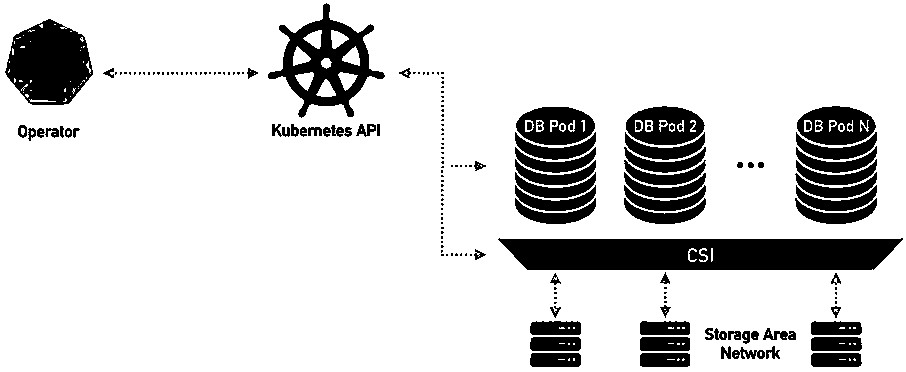
\includegraphics[width=11cm]{19_2019_Marzhan.jpg}
  %\caption{Statue of Liberty}	
  \label{fig1}
\end{figure}
\end{center}

To provide high availability operator uses node affinity to run PXC instances on separate worker nodes, with the automatical re-creation of the failed container on another node. Scheduled and on-demand backups can be done on any S3-compatible storage or stored locally. The operator also uses TLS cryptographic protocol as for internal communications (between PXC instances in the cluster) and external ones (between the client application and ProxySQL).

The MySQL Operator from Oracle uses a similar approach and is based on MySQL InnoDB Cluster \cite{bib3}. It provides scheduled and on-demand backups and restore, and uses Kubernetes Persistent Volume Claims to store data on local disk or network-attached storage. It is also able to use Prometheus to gather monitoring metrics.

\begin{thebibliography}{9}
\bibitem{bib1} presslabs/mysql-operator: Bulletproof MySQL on Kubernetes using Percona Server \url{https://github.com/presslabs/mysql-operator}
\bibitem{bib2} percona/percona-xtradb-cluster-operator: Percona Kubernetes Operator for XtraDB Cluster \url{https://github.com/percona/percona-xtradb-cluster-operator}
\bibitem{bib3} oracle/mysql-operator: Create, operate and scale self-healing MySQL clusters in Kubernetes \url{https://github.com/oracle/mysql-operator}
\bibitem{bib4} github/orchestrator: MySQL replication topology management and HA. \url{https://github.com/github/orchestrator}
\bibitem{bib5} Prometheus -- Monitoring system \& time-series database. \url{https://prometheus.io/}
\bibitem{bib6} Percona Monitoring and Management Documentation \url{https://www.percona.com/doc/percona-monitoring-and-management}
\bibitem{bib7} Percona XtraDB Cluster 5.7 Documentation \url{https://www.percona.com/doc/percona-xtradb-cluster}
\end{thebibliography}
\end{document}

\documentclass[10pt, a5paper]{article}
\usepackage{pdfpages}
\usepackage{parallel}
\usepackage[T2A]{fontenc}
\usepackage{ucs}
\usepackage[utf8x]{inputenc}
\usepackage[polish,english,russian]{babel}
\usepackage{hyperref}
\usepackage{rotating}
\usepackage[inner=2cm,top=1.8cm,outer=2cm,bottom=2.3cm,nohead]{geometry}
\usepackage{listings}
\usepackage{graphicx}
\usepackage{wrapfig}
\usepackage{longtable}
\usepackage{indentfirst}
\usepackage{array}
\newcolumntype{P}[1]{>{\raggedright\arraybackslash}p{#1}}
\frenchspacing
\usepackage{fixltx2e} %text sub- and superscripts
\usepackage{icomma} % коскі ў матэматычным рэжыме
\PreloadUnicodePage{4}

\newcommand{\longpage}{\enlargethispage{\baselineskip}}
\newcommand{\shortpage}{\enlargethispage{-\baselineskip}}

\def\switchlang#1{\expandafter\csname switchlang#1\endcsname}
\def\switchlangbe{
\let\saverefname=\refname%
\def\refname{Літаратура}%
\def\figurename{Іл.}%
}
\def\switchlangen{
\let\saverefname=\refname%
\def\refname{References}%
\def\figurename{Fig.}%
}
\def\switchlangru{
\let\saverefname=\refname%
\let\savefigurename=\figurename%
\def\refname{Литература}%
\def\figurename{Рис.}%
}

\hyphenation{admi-ni-stra-tive}
\hyphenation{ex-pe-ri-ence}
\hyphenation{fle-xi-bi-li-ty}
\hyphenation{Py-thon}
\hyphenation{ma-the-ma-ti-cal}
\hyphenation{re-ported}
\hyphenation{imp-le-menta-tions}
\hyphenation{pro-vides}
\hyphenation{en-gi-neering}
\hyphenation{com-pa-ti-bi-li-ty}
\hyphenation{im-pos-sible}
\hyphenation{desk-top}
\hyphenation{elec-tro-nic}
\hyphenation{com-pa-ny}
\hyphenation{de-ve-lop-ment}
\hyphenation{de-ve-loping}
\hyphenation{de-ve-lop}
\hyphenation{da-ta-ba-se}
\hyphenation{plat-forms}
\hyphenation{or-ga-ni-za-tion}
\hyphenation{pro-gramming}
\hyphenation{in-stru-ments}
\hyphenation{Li-nux}
\hyphenation{sour-ce}
\hyphenation{en-vi-ron-ment}
\hyphenation{Te-le-pathy}
\hyphenation{Li-nux-ov-ka}
\hyphenation{Open-BSD}
\hyphenation{Free-BSD}
\hyphenation{men-ti-on-ed}
\hyphenation{app-li-ca-tion}

\def\progref!#1!{\texttt{#1}}
\renewcommand{\arraystretch}{2} %Іначай формулы ў матрыцы зліпаюцца з лініямі
\usepackage{array}

\def\interview #1 (#2), #3, #4, #5\par{

\section[#1, #3, #4]{#1 -- #3, #4}
\def\qname{LVEE}
\def\aname{#1}
\def\q ##1\par{{\noindent \bf \qname: ##1 }\par}
\def\a{{\noindent \bf \aname: } \def\qname{L}\def\aname{#2}}
}

\def\interview* #1 (#2), #3, #4, #5\par{

\section*{#1\\{\small\rm #3, #4. #5}}

\def\qname{LVEE}
\def\aname{#1}
\def\q ##1\par{{\noindent \bf \qname: ##1 }\par}
\def\a{{\noindent \bf \aname: } \def\qname{L}\def\aname{#2}}
}

\switchlang{en}
\begin{document}
\title{Using eye trackers for the oculographic research in GNU/Linux}
\author{Dmitriy Kostiuk, Anastasia Markina, Brest, Belarus\footnote{\url{asyamarkina2@gmail.com}, \url {https://lvee.org/ru/abstracts/322}}}
\maketitle
\begin{abstract}
The analysis of oculography is presented taking into account the physiological and psychological characteristics of a person, as well as possible ways of using modern oculographic devices (eye trackers) to track the user's gaze direction in GNU/Linux. The overview of the features and performance of both software and hardware implementations is given. An experimental scheme used by the authors to study user interaction with graphical applications in GNU/Linux is discussed. The limitations and interpretation specifics are discussed.
\end{abstract}
When interacting with modern software, vision plays the role of the main, and in some cases, the only channel for perceiving information. At the same time, the clear and detailed vision provided by the central part of the retina covers an extremely small area, but half of the information processing is dedicated to it. Accordingly, detailed information is \linebreak obtained using visual sampling and scanning \cite{bib1}.

Oculographic research involves the analysis of the gaze movement and the areas of visual focalization on which the gaze is concentrated. Its application to assess the effectiveness of human-machine interaction can be divided into three categories \cite{bib2}:

\begin{itemize}
  \item identification of sources of difficulties (time-consuming form filling, etc.), in particular, related to the noticeability of elements, points of focus, mental stress and distractions;
  \item identification of specifics of user behavior (visual search strategies, reading and scanning patterns);
  \item comparison of several design decisions in conjunction with other types of testing (questionnaire, another biometric assessment).
\end{itemize}

Modern eye trackers typically use digital cameras that record the user's eye movements. The tracker is mounted on the user's head or is stationary fixed in the field of view.

Developers who wish to perform the oculographic testing of GNU/ Linux software have several options. The most budget option is the face and eye recognition using a webcam. This approach is implemented in such free projects as eviacam, TrackEye, WebGazer.js. They can be used to track gaze \cite{bib3}, but the result is very limited due to the webcam: it has a low frame rate and effective gaze positioning accuracy (half the resolution of the camera), and it is also difficult to recognize head rotation. Professional IT trackers, designed for research laboratories with a large budget (for some of them there are drivers for Linux) are on the opposite end of the scale. And there is a compromise solution, eye trackers that are targeted at the entertainment area but have accuracy sufficient for research tasks [4, 5]. We used together with GNU/Linux the eye trackers of this compromised category, produced by Tobii.

Tobii eye trackers are divided into the expensive Tobii Pro \linebreak professional series and consumer segment devices, for which the \linebreak manufacturer offers two types of SDKs: a low-level Stream Engine (declared to support Linux) and a higher-level Core SDK. We have tested two eye trackers, Tobii REX и Tobii EyeX. The alpha version of Stream Engine for Linux appeared only in 2018, and before there was a low-level Gaze SDK for Linux, which is currently not provided by the company.

\begin{center}
\begin{figure}[h!]
  \centering
  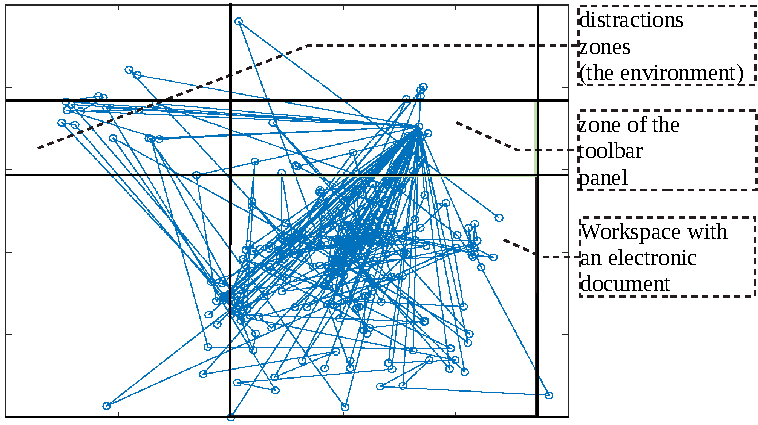
\includegraphics[width=10cm]{Markina1}
  \caption{User's gaze fixations when working with the application}	
  \label{markina:fig1}
\end{figure}
\end{center}

As a result of work, the eye tracker produces an array of coordinates corresponding to the position of the gaze at various points in time. Central vision provides information about the fine details of the image, but covers a relatively small part of the field of view; as a result, information is received using visual sampling, and peripheral vision indicates the next point of focus \cite{bib5}. The gaze moves with rapid leaps (saccades) with short pauses between them (fixations). So, when working with text, 7–9 letters are read in one saccade, and the fixation time is about 250 milliseconds, but the perception extends to twice as many letters due to peripheral vision \cite{bib7}. However, in the study of eye \linebreak movements, only central vision is recorded, and peripheral is not taken into account.

Visualization of the results of eye-tracking provides two options:

\begin{itemize}
  \item building a heat map, highlighting parts of the screen depending on the intensity of fixing the gaze;
  \item time-lapse mapping.
\end{itemize}

In both cases, the map is superimposed on the image of the user's working screen. When processing in GNU/Linux, it is convenient to use GNU Octave with a two-dimensional nuclear density estimation function to create heat maps by coordinates \cite{bib8}, and in case of a gaze map, one can just draw a graph in Graphviz, or also in Octave (see Fig. \ref{markina:fig1}, which illustrates the user’s work with a typical office application).

The parameters of descriptive statistics characterizing the shift of the distribution center are also informative when evaluating the results of the experiment (Fig. \ref{markina:fig2}): it is advisable, first of all, to select the middle region through which the gaze passes, calculate the median, the average value of the coordinates of the point where the gaze was fixed, and also determine the point at which the user most often focused his eyes, using mode.

If necessary, the percentage of eye fixations on individual functional parts of the application window (for example, the toolbar) and eye fixations outside the window (distraction area) can serve as simple numerical estimates of human-machine interactions obtained based on eye tracker data.

It is also necessary to take into account that there are physiological limitations due to which this technique cannot be applied: for example, nystagmus, which is characterized by involuntary eye movements with a high frequency, as a result of which the brain receives a fuzzy image of the object, and the eye tracker is not able to catch eye gaze.

\begin{center}
\begin{figure}[h!]
  \centering
  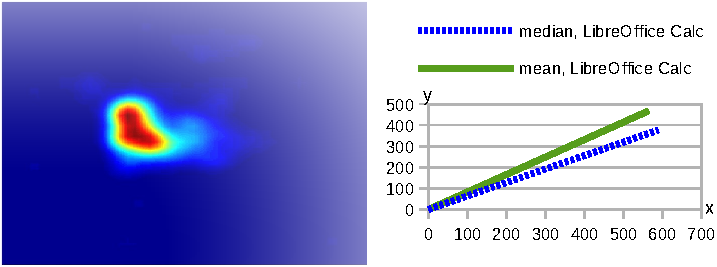
\includegraphics[width=10cm]{Markina2}
  \caption{Typical heatmap for gaze focalization (left) and shift of the distribution center of the sample (right) by the example of the table processor usage}	
  \label{markina:fig2}
\end{figure}
\end{center}


\begin{thebibliography}{9}
\bibitem{bib1} Titz J., Scholz A., Sedlmeier P. Comparing eye trackers by correlating their eye-metric data // Behav. Res., 2017.\url{https://www.ncbi.nlm.nih.gov/pubmed/28879442}
\bibitem{bib2} Дубицкий А., Костюк Д., Маркина А., Фомин С. Применение айтрекеров для юзабилити-исследований ПО в GNU/Linux // Четырнадцатая конференция разработчиков свободных программ: тезисы докладов – Калуга, 22–24 сентября 2017 г. – М. : Базальт СПО, 2017. – С. 36–41.
\bibitem{bib3} Semmelmann K., Weigelt S. Online webcam-based eye tracking in cognitive science: A first look // Behav. Res. 2017. \url{http://rdcu.be/tjzF.23}
\bibitem{bib4} Gibaldi A. et al. Evaluation of the Tobii EyeX Eye tracking controller and Matlab toolkit for research // Behav. Res. V. 49, 2017. P.923–946.
\bibitem{bib5} Ludwig C.J.H., Davies J.R., Eckstein M.P. Foveal Analysis and Peripheral Selection during Active Visual Sampling. // Proc. of the National Academy of Sciences of the USA. V. 111(2), 2014. P. E291–E299.
\bibitem{bib6} Goodman K.S. On Reading. / Portsmouth, NH: Heinemann, 1996. 152 p.
\bibitem{bib7} Ulloa A. Auto Heat Mapper. \url{https://github.com/aulloa/Auto_Heat_Mapper}
\end{thebibliography}
\end{document}

%\documentclass[10pt, a5paper]{article}
\usepackage{pdfpages}
\usepackage{parallel}
\usepackage[T2A]{fontenc}
\usepackage{ucs}
\usepackage[utf8x]{inputenc}
\usepackage[polish,english,russian]{babel}
\usepackage{hyperref}
\usepackage{rotating}
\usepackage[inner=2cm,top=1.8cm,outer=2cm,bottom=2.3cm,nohead]{geometry}
\usepackage{listings}
\usepackage{graphicx}
\usepackage{wrapfig}
\usepackage{longtable}
\usepackage{indentfirst}
\usepackage{array}
\newcolumntype{P}[1]{>{\raggedright\arraybackslash}p{#1}}
\frenchspacing
\usepackage{fixltx2e} %text sub- and superscripts
\usepackage{icomma} % коскі ў матэматычным рэжыме
\PreloadUnicodePage{4}

\newcommand{\longpage}{\enlargethispage{\baselineskip}}
\newcommand{\shortpage}{\enlargethispage{-\baselineskip}}

\def\switchlang#1{\expandafter\csname switchlang#1\endcsname}
\def\switchlangbe{
\let\saverefname=\refname%
\def\refname{Літаратура}%
\def\figurename{Іл.}%
}
\def\switchlangen{
\let\saverefname=\refname%
\def\refname{References}%
\def\figurename{Fig.}%
}
\def\switchlangru{
\let\saverefname=\refname%
\let\savefigurename=\figurename%
\def\refname{Литература}%
\def\figurename{Рис.}%
}

\hyphenation{admi-ni-stra-tive}
\hyphenation{ex-pe-ri-ence}
\hyphenation{fle-xi-bi-li-ty}
\hyphenation{Py-thon}
\hyphenation{ma-the-ma-ti-cal}
\hyphenation{re-ported}
\hyphenation{imp-le-menta-tions}
\hyphenation{pro-vides}
\hyphenation{en-gi-neering}
\hyphenation{com-pa-ti-bi-li-ty}
\hyphenation{im-pos-sible}
\hyphenation{desk-top}
\hyphenation{elec-tro-nic}
\hyphenation{com-pa-ny}
\hyphenation{de-ve-lop-ment}
\hyphenation{de-ve-loping}
\hyphenation{de-ve-lop}
\hyphenation{da-ta-ba-se}
\hyphenation{plat-forms}
\hyphenation{or-ga-ni-za-tion}
\hyphenation{pro-gramming}
\hyphenation{in-stru-ments}
\hyphenation{Li-nux}
\hyphenation{sour-ce}
\hyphenation{en-vi-ron-ment}
\hyphenation{Te-le-pathy}
\hyphenation{Li-nux-ov-ka}
\hyphenation{Open-BSD}
\hyphenation{Free-BSD}
\hyphenation{men-ti-on-ed}
\hyphenation{app-li-ca-tion}

\def\progref!#1!{\texttt{#1}}
\renewcommand{\arraystretch}{2} %Іначай формулы ў матрыцы зліпаюцца з лініямі
\usepackage{array}

\def\interview #1 (#2), #3, #4, #5\par{

\section[#1, #3, #4]{#1 -- #3, #4}
\def\qname{LVEE}
\def\aname{#1}
\def\q ##1\par{{\noindent \bf \qname: ##1 }\par}
\def\a{{\noindent \bf \aname: } \def\qname{L}\def\aname{#2}}
}

\def\interview* #1 (#2), #3, #4, #5\par{

\section*{#1\\{\small\rm #3, #4. #5}}

\def\qname{LVEE}
\def\aname{#1}
\def\q ##1\par{{\noindent \bf \qname: ##1 }\par}
\def\a{{\noindent \bf \aname: } \def\qname{L}\def\aname{#2}}
}

%\frenchspacing
\begin{document}
\title{Голос спонсора: ITS Partner}
%\author{}
\date{}
\maketitle%

~

\end{document}




%\documentclass[10pt, a5paper]{article}
\usepackage{pdfpages}
\usepackage{parallel}
\usepackage[T2A]{fontenc}
\usepackage{ucs}
\usepackage[utf8x]{inputenc}
\usepackage[polish,english,russian]{babel}
\usepackage{hyperref}
\usepackage{rotating}
\usepackage[inner=2cm,top=1.8cm,outer=2cm,bottom=2.3cm,nohead]{geometry}
\usepackage{listings}
\usepackage{graphicx}
\usepackage{wrapfig}
\usepackage{longtable}
\usepackage{indentfirst}
\usepackage{array}
\newcolumntype{P}[1]{>{\raggedright\arraybackslash}p{#1}}
\frenchspacing
\usepackage{fixltx2e} %text sub- and superscripts
\usepackage{icomma} % коскі ў матэматычным рэжыме
\PreloadUnicodePage{4}

\newcommand{\longpage}{\enlargethispage{\baselineskip}}
\newcommand{\shortpage}{\enlargethispage{-\baselineskip}}

\def\switchlang#1{\expandafter\csname switchlang#1\endcsname}
\def\switchlangbe{
\let\saverefname=\refname%
\def\refname{Літаратура}%
\def\figurename{Іл.}%
}
\def\switchlangen{
\let\saverefname=\refname%
\def\refname{References}%
\def\figurename{Fig.}%
}
\def\switchlangru{
\let\saverefname=\refname%
\let\savefigurename=\figurename%
\def\refname{Литература}%
\def\figurename{Рис.}%
}

\hyphenation{admi-ni-stra-tive}
\hyphenation{ex-pe-ri-ence}
\hyphenation{fle-xi-bi-li-ty}
\hyphenation{Py-thon}
\hyphenation{ma-the-ma-ti-cal}
\hyphenation{re-ported}
\hyphenation{imp-le-menta-tions}
\hyphenation{pro-vides}
\hyphenation{en-gi-neering}
\hyphenation{com-pa-ti-bi-li-ty}
\hyphenation{im-pos-sible}
\hyphenation{desk-top}
\hyphenation{elec-tro-nic}
\hyphenation{com-pa-ny}
\hyphenation{de-ve-lop-ment}
\hyphenation{de-ve-loping}
\hyphenation{de-ve-lop}
\hyphenation{da-ta-ba-se}
\hyphenation{plat-forms}
\hyphenation{or-ga-ni-za-tion}
\hyphenation{pro-gramming}
\hyphenation{in-stru-ments}
\hyphenation{Li-nux}
\hyphenation{sour-ce}
\hyphenation{en-vi-ron-ment}
\hyphenation{Te-le-pathy}
\hyphenation{Li-nux-ov-ka}
\hyphenation{Open-BSD}
\hyphenation{Free-BSD}
\hyphenation{men-ti-on-ed}
\hyphenation{app-li-ca-tion}

\def\progref!#1!{\texttt{#1}}
\renewcommand{\arraystretch}{2} %Іначай формулы ў матрыцы зліпаюцца з лініямі
\usepackage{array}

\def\interview #1 (#2), #3, #4, #5\par{

\section[#1, #3, #4]{#1 -- #3, #4}
\def\qname{LVEE}
\def\aname{#1}
\def\q ##1\par{{\noindent \bf \qname: ##1 }\par}
\def\a{{\noindent \bf \aname: } \def\qname{L}\def\aname{#2}}
}

\def\interview* #1 (#2), #3, #4, #5\par{

\section*{#1\\{\small\rm #3, #4. #5}}

\def\qname{LVEE}
\def\aname{#1}
\def\q ##1\par{{\noindent \bf \qname: ##1 }\par}
\def\a{{\noindent \bf \aname: } \def\qname{L}\def\aname{#2}}
}

\begin{document}
\title{Голос спонсора: SaM Solutions}
%\author{}
\date{}
\maketitle

Компания SaM Solutions выступает в роли системо-образующего спонсора конференции Linux Vacation Eastern Europe с момента рождения LVEE в 2005 году и на протяжении всех лет её проведения. 

Сложившаяся корпоративная практика не случайна. Продукты и решения, задействующие Linux и другие Free/Open Source Software проекты, составляют заметную часть пакета разработок SaM Solutions. Кадровая политика компании направлена на поощрение профессионального развития своих сотрудников, организацию их эффективного отдыха и привлечение хорошо мотивированных кандидатов к работе на компанию. Формат конференции LVEE успешно позволяет решать все три задачи. 

Одним из подразделений компании является отдел Linux и \linebreak Embbeded. Специалисты компании на протяжении десятилетий работают с СПО. Компанией реализован ряд проектов по адаптации ОС GNU/Linux для работы в различных устройствах, построенных на таких платформах как ARM, PowerPC, x86, MIPS. В последние годы "--- на ведущие позиции выходит разработка управляющего ПО для серверов Enterprise-класса, от низкоуровнего BMC Firmware на основе Linux до высокоуровневых систем контроля виртуализации и графических интерфейсов управления, от прошивок устройств хранения данных до BSP интегрированных плат для разработчика. Надёжность, качество и широкая функциональность множества свободных проектов позволяет строить нам системы любого уровня и сложности, опираясь на высококачественные готовые компоненты.

В рамках направления Linux и Embedded успешно выполнены проекты для таких знаковых заказчиков, как  Novell/SUSE, Fujitsu Technology Solutions  и осуществляется партнёрство с компаниями IBM и Oracle/Sun в области Open Source решений.

Мы разрабатываем, модифицируем и адаптируем различное свободное программное обеспечение для наших заказчиков, но не забываем и о своих нуждах "--- наши сотрудники используют в своей работе существующие програмные продукты и вносят вклад в их развитие. Часть внутренней инфраструктуры, а именно интранет-сеть компании, тестовые стенды отдела контроля качества, рабочие места сотрудников профильных подразделений "--- также работает под управлением СПО (серверные и десктопные платформы GNU/Linux и FreeBSD). 

В минувшем году, в рамках реорганизации, был разработан долгосрочный план развития направления Linux и Embedded в SaM Solutions. В нём впервые были кодифицированы уже имеющиеся внутренние неофициальные практики по взаимодействию с commu"=nity-based проектами. В частности разработаны меры и правила по
\begin{itemize}
  \item возврата изменений в родительские проекты (upstreaming);
  \item вхождения в состав постоянных разработчиков активно используемых нами FOSS-компонентов;
  \item публикации сообщений об ошибках (bug reporting);
  \item участия и помощи в организации community events;
  \item стимуляции докладов и участия в технических конференциях.
\end{itemize}
И план немедленно начал претворяться в жизнь.

Силами отдела организовано внутреннее обучение сотрудников на регулярной
основе. Был прочтен и опубликован курс по TDD. По согласованию с автором
опубликован курс Debian/Ubuntu Packaging (видео, презентация и исходные
тексты презентации в \LaTeX).  Были организованы и проведены курсы по
обучению QA специалистов для направления Embeded Linux. Проведено
практическое занятие по основам виртуализации и эмуляции, организована
лекция по вопросу профилирования и оптимизации Ruby-кода, лекция о
High-availability кластерах и направлении развития технологии. Кроме того,
проводился семинар по Video4Linux2. Для создания и обучения кадрового
резерва на ближайшее будущее запланированы постоянно действующие внутренние
проекты в области Embedded Linux, результаты которых также запланированы к
публикации.

Визиты представительных делегаций на Embedded World 2012 и Linux Con Europe/Embedded LinuxCon Europe 2011 обогатили нас новыми идеями, куда можно
двигаться дальше и что сейчас актуально. А выступления на Software
Engineering Forum for Students, круглом столе по СПО в рамках TIBO-2012
и LVEE Winter 2012 позволили поделиться опытом с
заинтересованными сторонами.

В апреле состоялась Ганноверская промышленная ярмарка \linebreak (Hannover Messe
2013). Компания SaM Solutions была представлена отдельным стендом, на
котором демонстрировались наработки в области встроенного и системного ПО
на базе OS Linux. Идея «умного» дома вызвала неподдельный интерес у
посетителей стенда.

При поддержке SaM Solutions, с декабря 2011 года возобновились регулярные встречи Minsk Linux Users Groups, под названием <<Линуксовка в SaM Solutions>>. Техническое оснащение линуксовок и открытый формат встреч позволил им практически мгновенно стать заметным дискуссионным клубом по широкому спектру вопросов, прямо или косвенно связанных с СПО. Свободная картография (OpenStreetMap), технологии виртуализации, минский \linebreak hackerspace, Linux Mobile, бойкот Голливудской продукции, systemd, загрузчик u-boot, белорусская локализация GNOME --- это только часть тем, поднятых за последние линуксовки.

Быстрые и положительные изменения, как внутри компании SaM Solutions, так и в экосфере СПО (и Linux в частности) наполняют нас уверенностью, что направление движения выбрано верно.

\begin{figure}[h!]
\centering
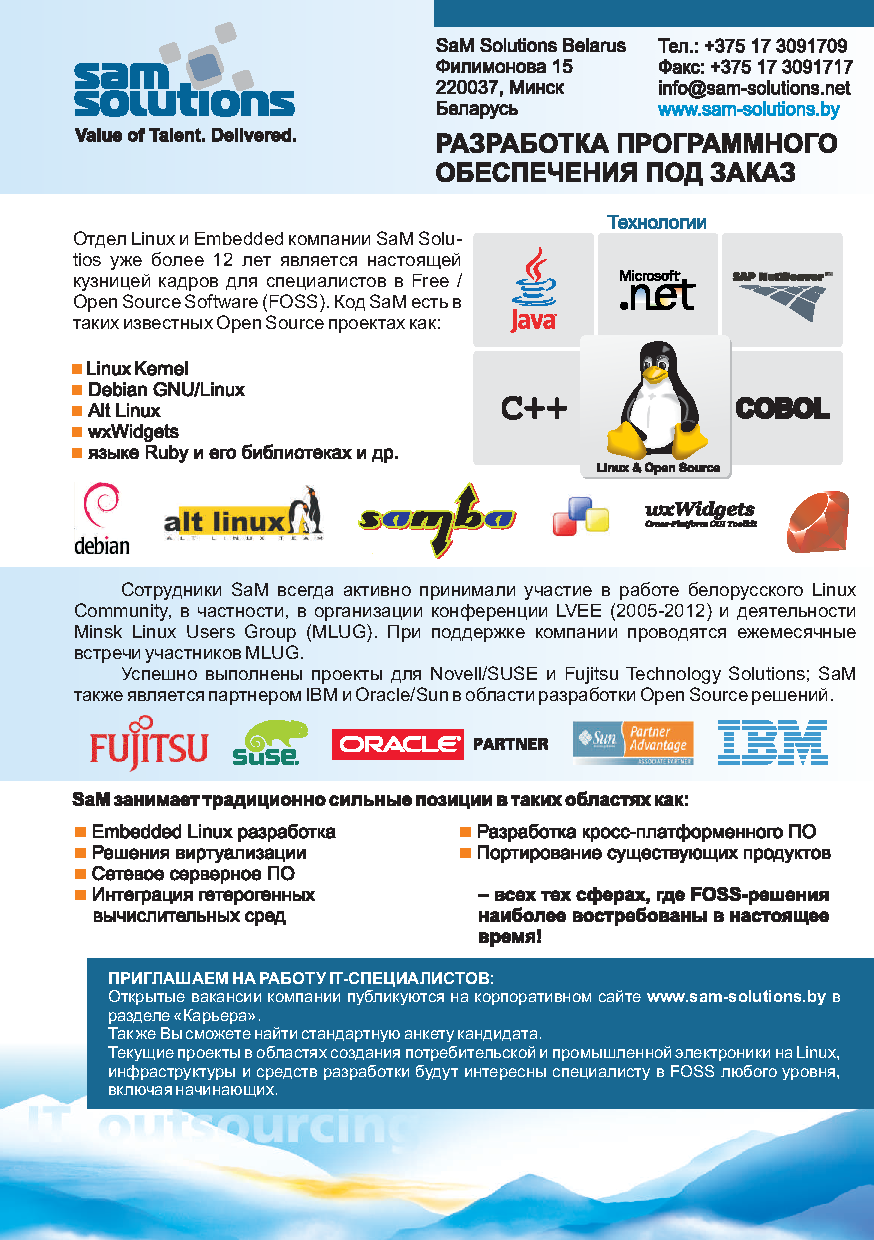
\includegraphics[height=11.8cm]{48_spons_sams.pdf}
\end{figure}
\end{document}



%\documentclass[10pt, a5paper]{article}
\usepackage{pdfpages}
\usepackage{parallel}
\usepackage[T2A]{fontenc}
\usepackage{ucs}
\usepackage[utf8x]{inputenc}
\usepackage[polish,english,russian]{babel}
\usepackage{hyperref}
\usepackage{rotating}
\usepackage[inner=2cm,top=1.8cm,outer=2cm,bottom=2.3cm,nohead]{geometry}
\usepackage{listings}
\usepackage{graphicx}
\usepackage{wrapfig}
\usepackage{longtable}
\usepackage{indentfirst}
\usepackage{array}
\newcolumntype{P}[1]{>{\raggedright\arraybackslash}p{#1}}
\frenchspacing
\usepackage{fixltx2e} %text sub- and superscripts
\usepackage{icomma} % коскі ў матэматычным рэжыме
\PreloadUnicodePage{4}

\newcommand{\longpage}{\enlargethispage{\baselineskip}}
\newcommand{\shortpage}{\enlargethispage{-\baselineskip}}

\def\switchlang#1{\expandafter\csname switchlang#1\endcsname}
\def\switchlangbe{
\let\saverefname=\refname%
\def\refname{Літаратура}%
\def\figurename{Іл.}%
}
\def\switchlangen{
\let\saverefname=\refname%
\def\refname{References}%
\def\figurename{Fig.}%
}
\def\switchlangru{
\let\saverefname=\refname%
\let\savefigurename=\figurename%
\def\refname{Литература}%
\def\figurename{Рис.}%
}

\hyphenation{admi-ni-stra-tive}
\hyphenation{ex-pe-ri-ence}
\hyphenation{fle-xi-bi-li-ty}
\hyphenation{Py-thon}
\hyphenation{ma-the-ma-ti-cal}
\hyphenation{re-ported}
\hyphenation{imp-le-menta-tions}
\hyphenation{pro-vides}
\hyphenation{en-gi-neering}
\hyphenation{com-pa-ti-bi-li-ty}
\hyphenation{im-pos-sible}
\hyphenation{desk-top}
\hyphenation{elec-tro-nic}
\hyphenation{com-pa-ny}
\hyphenation{de-ve-lop-ment}
\hyphenation{de-ve-loping}
\hyphenation{de-ve-lop}
\hyphenation{da-ta-ba-se}
\hyphenation{plat-forms}
\hyphenation{or-ga-ni-za-tion}
\hyphenation{pro-gramming}
\hyphenation{in-stru-ments}
\hyphenation{Li-nux}
\hyphenation{sour-ce}
\hyphenation{en-vi-ron-ment}
\hyphenation{Te-le-pathy}
\hyphenation{Li-nux-ov-ka}
\hyphenation{Open-BSD}
\hyphenation{Free-BSD}
\hyphenation{men-ti-on-ed}
\hyphenation{app-li-ca-tion}

\def\progref!#1!{\texttt{#1}}
\renewcommand{\arraystretch}{2} %Іначай формулы ў матрыцы зліпаюцца з лініямі
\usepackage{array}

\def\interview #1 (#2), #3, #4, #5\par{

\section[#1, #3, #4]{#1 -- #3, #4}
\def\qname{LVEE}
\def\aname{#1}
\def\q ##1\par{{\noindent \bf \qname: ##1 }\par}
\def\a{{\noindent \bf \aname: } \def\qname{L}\def\aname{#2}}
}

\def\interview* #1 (#2), #3, #4, #5\par{

\section*{#1\\{\small\rm #3, #4. #5}}

\def\qname{LVEE}
\def\aname{#1}
\def\q ##1\par{{\noindent \bf \qname: ##1 }\par}
\def\a{{\noindent \bf \aname: } \def\qname{L}\def\aname{#2}}
}

%\frenchspacing
\begin{document}
\title{Голос спонсора: ITS Partner}
%\author{}
\date{}
\maketitle

~

\newpage

~

\end{document}

%\documentclass[10pt, a5paper]{article}
\usepackage{pdfpages}
\usepackage{parallel}
\usepackage[T2A]{fontenc}
\usepackage{ucs}
\usepackage[utf8x]{inputenc}
\usepackage[polish,english,russian]{babel}
\usepackage{hyperref}
\usepackage{rotating}
\usepackage[inner=2cm,top=1.8cm,outer=2cm,bottom=2.3cm,nohead]{geometry}
\usepackage{listings}
\usepackage{graphicx}
\usepackage{wrapfig}
\usepackage{longtable}
\usepackage{indentfirst}
\usepackage{array}
\newcolumntype{P}[1]{>{\raggedright\arraybackslash}p{#1}}
\frenchspacing
\usepackage{fixltx2e} %text sub- and superscripts
\usepackage{icomma} % коскі ў матэматычным рэжыме
\PreloadUnicodePage{4}

\newcommand{\longpage}{\enlargethispage{\baselineskip}}
\newcommand{\shortpage}{\enlargethispage{-\baselineskip}}

\def\switchlang#1{\expandafter\csname switchlang#1\endcsname}
\def\switchlangbe{
\let\saverefname=\refname%
\def\refname{Літаратура}%
\def\figurename{Іл.}%
}
\def\switchlangen{
\let\saverefname=\refname%
\def\refname{References}%
\def\figurename{Fig.}%
}
\def\switchlangru{
\let\saverefname=\refname%
\let\savefigurename=\figurename%
\def\refname{Литература}%
\def\figurename{Рис.}%
}

\hyphenation{admi-ni-stra-tive}
\hyphenation{ex-pe-ri-ence}
\hyphenation{fle-xi-bi-li-ty}
\hyphenation{Py-thon}
\hyphenation{ma-the-ma-ti-cal}
\hyphenation{re-ported}
\hyphenation{imp-le-menta-tions}
\hyphenation{pro-vides}
\hyphenation{en-gi-neering}
\hyphenation{com-pa-ti-bi-li-ty}
\hyphenation{im-pos-sible}
\hyphenation{desk-top}
\hyphenation{elec-tro-nic}
\hyphenation{com-pa-ny}
\hyphenation{de-ve-lop-ment}
\hyphenation{de-ve-loping}
\hyphenation{de-ve-lop}
\hyphenation{da-ta-ba-se}
\hyphenation{plat-forms}
\hyphenation{or-ga-ni-za-tion}
\hyphenation{pro-gramming}
\hyphenation{in-stru-ments}
\hyphenation{Li-nux}
\hyphenation{sour-ce}
\hyphenation{en-vi-ron-ment}
\hyphenation{Te-le-pathy}
\hyphenation{Li-nux-ov-ka}
\hyphenation{Open-BSD}
\hyphenation{Free-BSD}
\hyphenation{men-ti-on-ed}
\hyphenation{app-li-ca-tion}

\def\progref!#1!{\texttt{#1}}
\renewcommand{\arraystretch}{2} %Іначай формулы ў матрыцы зліпаюцца з лініямі
\usepackage{array}

\def\interview #1 (#2), #3, #4, #5\par{

\section[#1, #3, #4]{#1 -- #3, #4}
\def\qname{LVEE}
\def\aname{#1}
\def\q ##1\par{{\noindent \bf \qname: ##1 }\par}
\def\a{{\noindent \bf \aname: } \def\qname{L}\def\aname{#2}}
}

\def\interview* #1 (#2), #3, #4, #5\par{

\section*{#1\\{\small\rm #3, #4. #5}}

\def\qname{LVEE}
\def\aname{#1}
\def\q ##1\par{{\noindent \bf \qname: ##1 }\par}
\def\a{{\noindent \bf \aname: } \def\qname{L}\def\aname{#2}}
}

%\frenchspacing
\begin{document}
\title{Голос спонсора: mycloud.by}
%\author{}
\date{}
\maketitle

~


\end{document}

\newpage
~ % SaMs 1
\newpage
~ % SaMs 2
%\documentclass[10pt, a5paper]{article}
\usepackage{pdfpages}
\usepackage{parallel}
\usepackage[T2A]{fontenc}
\usepackage{ucs}
\usepackage[utf8x]{inputenc}
\usepackage[polish,english,russian]{babel}
\usepackage{hyperref}
\usepackage{rotating}
\usepackage[inner=2cm,top=1.8cm,outer=2cm,bottom=2.3cm,nohead]{geometry}
\usepackage{listings}
\usepackage{graphicx}
\usepackage{wrapfig}
\usepackage{longtable}
\usepackage{indentfirst}
\usepackage{array}
\newcolumntype{P}[1]{>{\raggedright\arraybackslash}p{#1}}
\frenchspacing
\usepackage{fixltx2e} %text sub- and superscripts
\usepackage{icomma} % коскі ў матэматычным рэжыме
\PreloadUnicodePage{4}

\newcommand{\longpage}{\enlargethispage{\baselineskip}}
\newcommand{\shortpage}{\enlargethispage{-\baselineskip}}

\def\switchlang#1{\expandafter\csname switchlang#1\endcsname}
\def\switchlangbe{
\let\saverefname=\refname%
\def\refname{Літаратура}%
\def\figurename{Іл.}%
}
\def\switchlangen{
\let\saverefname=\refname%
\def\refname{References}%
\def\figurename{Fig.}%
}
\def\switchlangru{
\let\saverefname=\refname%
\let\savefigurename=\figurename%
\def\refname{Литература}%
\def\figurename{Рис.}%
}

\hyphenation{admi-ni-stra-tive}
\hyphenation{ex-pe-ri-ence}
\hyphenation{fle-xi-bi-li-ty}
\hyphenation{Py-thon}
\hyphenation{ma-the-ma-ti-cal}
\hyphenation{re-ported}
\hyphenation{imp-le-menta-tions}
\hyphenation{pro-vides}
\hyphenation{en-gi-neering}
\hyphenation{com-pa-ti-bi-li-ty}
\hyphenation{im-pos-sible}
\hyphenation{desk-top}
\hyphenation{elec-tro-nic}
\hyphenation{com-pa-ny}
\hyphenation{de-ve-lop-ment}
\hyphenation{de-ve-loping}
\hyphenation{de-ve-lop}
\hyphenation{da-ta-ba-se}
\hyphenation{plat-forms}
\hyphenation{or-ga-ni-za-tion}
\hyphenation{pro-gramming}
\hyphenation{in-stru-ments}
\hyphenation{Li-nux}
\hyphenation{sour-ce}
\hyphenation{en-vi-ron-ment}
\hyphenation{Te-le-pathy}
\hyphenation{Li-nux-ov-ka}
\hyphenation{Open-BSD}
\hyphenation{Free-BSD}
\hyphenation{men-ti-on-ed}
\hyphenation{app-li-ca-tion}

\def\progref!#1!{\texttt{#1}}
\renewcommand{\arraystretch}{2} %Іначай формулы ў матрыцы зліпаюцца з лініямі
\usepackage{array}

\def\interview #1 (#2), #3, #4, #5\par{

\section[#1, #3, #4]{#1 -- #3, #4}
\def\qname{LVEE}
\def\aname{#1}
\def\q ##1\par{{\noindent \bf \qname: ##1 }\par}
\def\a{{\noindent \bf \aname: } \def\qname{L}\def\aname{#2}}
}

\def\interview* #1 (#2), #3, #4, #5\par{

\section*{#1\\{\small\rm #3, #4. #5}}

\def\qname{LVEE}
\def\aname{#1}
\def\q ##1\par{{\noindent \bf \qname: ##1 }\par}
\def\a{{\noindent \bf \aname: } \def\qname{L}\def\aname{#2}}
}

\begin{document}
\title{Голос спонсора: EPAM Systems}
%\author{}
\date{}
\maketitle

Компания EPAM Systems не первый год является спонсором международной конференции разработчиков и пользователей свободного программного обеспечения LVEE (Linux Vacation / Eastern Europe). Этот год также не стал исключением. Пожалуй, LVEE является самым значимым событием для русскоязычных разработчиков и тестировщиков Open Source. Каждое лето здесь встречаются начинающие специалисты и «ветераны»"=разработчики из десятка стран для обмена опытом и общения на профессиональные темы. Наши специалисты также активно участвуют в данной конференции: в качестве докладчиков и организаторов/волонтёров. Это уникальная в своём роде конференция, и именно поэтому EPAM Systems очередной раз принимает участие в LVEE в качестве спонсора.


EPAM Systems "--- одна из крупнейших компаний"=поставщиков\linebreak услуг в области разработки программного обеспечения и решений на территории СНГ и Центральной и Восточной Европы. Созданная в 1993 году, сегодня она имеет представительства в 12 странах мира, в штате работают более 9 тыс. сотрудников, из которых более 3 тыс. "--- в Беларуси. Рост компании обеспечивается за счет собственных обучающих программ и передаче опыта от больших специалистов до начинающих разработчиков. Компания EPAM Systems выполняет проекты более чем в 30 странах мира. Основные направления деятельности: разработка, тестирование, сопровождение и поддержка заказного программного обеспечения и бизнес"=приложений, а также ИТ"=консалтинг с учетом отраслевой специфики бизнеса.

Наша компания участвует в проектах с такими крупными, хорошо известными заказчиками как Google, Novell, Infoblox, Parallels, 10Gen и др., так и с небольшими, в том числе и с начинающими свой путь в софтверном бизнесе.


К примеру, для Infoblox была реализована связка между WebUI с BIND и DHCP. Для этого был разработан комплекс решений под управлением Shell и Python скриптов, а также механизм позволяющий вносить правки в BIND и DHCP на языке C. Также был разработан развернутый функционал, автоматизирующий инсталляцию новых устройств и их эксплуатацию, что позволяет значительно упростить управление данными. Встроенный Web"=интерфейс позволяет разворачивать, управлять сервисами DNS, DNSSEC, DHCP, IPAM, устанавливать новые версии ПО, архивировать и восстанавливать из архивов необходимые данные, восстанавливать их после аварии, проводить мониторинг сети и создавать отчеты без необходимости обращения к командной строке.


Еще одним решением, реализованным для компании Infoblox, являлся программный продукт, позволяющий контролировать сетевые изменения, таким образом, облегчая идентификацию трудноуловимых проблем конфигурации и соответствие требованиям. Вместо того чтобы просто регистрировать изменения, система использует внесенную информацию для проверки, анализа и автоматической обработки сетевых изменений. Благодаря инновационной, квалифицированной, глубокой технике логического анализа, программа изолирует проблемы исправности и конфигурации до того, как они могут вызвать более серьезные сбои.


Разработанная для анализа сложных сетей система изучает сеть, собирает ключевую информацию, применяет встроенную технику логического анализа и создает оценку исправности сети и список проблем, требующих принятие мер для улучшения качества работы сети.


Правильное использование свободного ПО в разработках сокращает и расходы на покупку лицензионных программ, и трудозатраты при создании коммерческого ПО. Немалую роль для достижения превосходного результата играет привлечение к разработке опытных специалистов. LVEE способствует появлению таких специалистов, развитию их навыков и расширению кругозора. Хотелось бы пожелать участникам конференции интересных проектов и максимум пользы от участия в LVEE.


\end{document}



\documentclass[10pt, a5paper]{article}
\usepackage{pdfpages}
\usepackage{parallel}
\usepackage[T2A]{fontenc}
\usepackage{ucs}
\usepackage[utf8x]{inputenc}
\usepackage[polish,english,russian]{babel}
\usepackage{hyperref}
\usepackage{rotating}
\usepackage[inner=2cm,top=1.8cm,outer=2cm,bottom=2.3cm,nohead]{geometry}
\usepackage{listings}
\usepackage{graphicx}
\usepackage{wrapfig}
\usepackage{longtable}
\usepackage{indentfirst}
\usepackage{array}
\newcolumntype{P}[1]{>{\raggedright\arraybackslash}p{#1}}
\frenchspacing
\usepackage{fixltx2e} %text sub- and superscripts
\usepackage{icomma} % коскі ў матэматычным рэжыме
\PreloadUnicodePage{4}

\newcommand{\longpage}{\enlargethispage{\baselineskip}}
\newcommand{\shortpage}{\enlargethispage{-\baselineskip}}

\def\switchlang#1{\expandafter\csname switchlang#1\endcsname}
\def\switchlangbe{
\let\saverefname=\refname%
\def\refname{Літаратура}%
\def\figurename{Іл.}%
}
\def\switchlangen{
\let\saverefname=\refname%
\def\refname{References}%
\def\figurename{Fig.}%
}
\def\switchlangru{
\let\saverefname=\refname%
\let\savefigurename=\figurename%
\def\refname{Литература}%
\def\figurename{Рис.}%
}

\hyphenation{admi-ni-stra-tive}
\hyphenation{ex-pe-ri-ence}
\hyphenation{fle-xi-bi-li-ty}
\hyphenation{Py-thon}
\hyphenation{ma-the-ma-ti-cal}
\hyphenation{re-ported}
\hyphenation{imp-le-menta-tions}
\hyphenation{pro-vides}
\hyphenation{en-gi-neering}
\hyphenation{com-pa-ti-bi-li-ty}
\hyphenation{im-pos-sible}
\hyphenation{desk-top}
\hyphenation{elec-tro-nic}
\hyphenation{com-pa-ny}
\hyphenation{de-ve-lop-ment}
\hyphenation{de-ve-loping}
\hyphenation{de-ve-lop}
\hyphenation{da-ta-ba-se}
\hyphenation{plat-forms}
\hyphenation{or-ga-ni-za-tion}
\hyphenation{pro-gramming}
\hyphenation{in-stru-ments}
\hyphenation{Li-nux}
\hyphenation{sour-ce}
\hyphenation{en-vi-ron-ment}
\hyphenation{Te-le-pathy}
\hyphenation{Li-nux-ov-ka}
\hyphenation{Open-BSD}
\hyphenation{Free-BSD}
\hyphenation{men-ti-on-ed}
\hyphenation{app-li-ca-tion}

\def\progref!#1!{\texttt{#1}}
\renewcommand{\arraystretch}{2} %Іначай формулы ў матрыцы зліпаюцца з лініямі
\usepackage{array}

\def\interview #1 (#2), #3, #4, #5\par{

\section[#1, #3, #4]{#1 -- #3, #4}
\def\qname{LVEE}
\def\aname{#1}
\def\q ##1\par{{\noindent \bf \qname: ##1 }\par}
\def\a{{\noindent \bf \aname: } \def\qname{L}\def\aname{#2}}
}

\def\interview* #1 (#2), #3, #4, #5\par{

\section*{#1\\{\small\rm #3, #4. #5}}

\def\qname{LVEE}
\def\aname{#1}
\def\q ##1\par{{\noindent \bf \qname: ##1 }\par}
\def\a{{\noindent \bf \aname: } \def\qname{L}\def\aname{#2}}
}

%\switchlang{be}
%\usepackage{color}
\begin{document}
\title{Интервью}
%\author{}
\date{}
\maketitle

\begin{Parallel}[p]{}{}

     \ParallelLText{%
      \selectlanguage{english}
\interview* Bjarne Stroustrup (BS.), New York, USA,

{\noindent \bf LVEE: Tell us something about your first experience with the open-source software. 
Perhaps the earlier experience took place in times of large computers when being open source was typical. But it would be also interesting to know something about your first experience with free/libre licensed software (something ideologically positioned in term of freedom). Maybe it was GCC, but who knows :)} 

{\noindent \bf BS:} I suspect my first encounter was at the first USENIX C++ conference in Santa Fe when Michael Tiemann gave a talk about how his new compiler GCC was going to do every conceivable compiler trick and soon put all other compilers out of business with his new G++ dialect. I was somewhat amused and GCC did eventually become a major factor in the C++ world, but it was several years before I could accept GCC as a C++ compiler. Before 2.95, it simply couldn’t compile any program I really cared about. The early versions had many features missing and several peculiar extensions.

I am not keen on GPL because I don’t see all software becoming open-source. For starters there is a lot of software that is too complex and too specialized to attract maintainers. I prefer – and use – the more liberal MIT license. The GPL library license that Michael Tiemann created to make it possible for non-ideologically-motivated organizations to use GCC and its standard library commercially was a major improvement. I think that without the LGPL, GCC and C++ would have been far less of an asset to the greater Linux community.

Generally, I try to stay out of political discussions.

{\noindent \bf L: You have already mentioned in some of your previous interviews that you prefer the diversity of the operating systems and compilers.}

{\noindent \bf BS:} I strongly prefer diversity of operating systems, languages, and implementations. That is partly because I fear monocultures. I wouldn’t even like my favorite OS or programming language to become so dominant that the people who controlled it could become a burden on the community and/or a single point of failure. Having multiple suppliers of a technology is a good defense against stagnation.

For example, the competition from Clang has vastly improved GCC and Microsoft’s C++ compiler. 

{\noindent \bf L: As a conference, Linux Vacation / Eastern Europe is dedicated to a wide range of open source technologies, but it includes ``Linux'' in its name, so one of the most obvious questions is the following: which GNU/Linux distros have you mostly used? Maybe there is some distro which is more convenient for your working habits now (also, it would be interesting to know about your current usage of other Unix and Unix-like systems, if any). }

{\noindent \bf BS:} At work, I use Red Hat Linux. On my (Windows) Laptop, I have Ubuntu. My academic computer runs CentOS. I try hard to stay portable and to think of them all as Unix.

{\noindent \bf L: Beside Unix, you've previously worked a lot in Plan9 OS (which is something esoteric for absolute majority of our participants), so it is interesting, how would you characterize Plan9 GUI from the contemporary point of view.}

{\noindent \bf BS:} I was merely a – happy – user of Plan9. I did not develop for it. I still consider “Sam” the nicest editor I have ever used.

{\noindent \bf L: Can you briefly name features of the Sam editor which you liked? The fact that you actively used Sam is mentioned in Wikipedia, but there without any details about things you liked it for.}

{\noindent \bf BS:} It was simple, very easy to use, and fast. I mostly liked what it didn’t have: no modes or complicated commands, just cut, paste, snarf, and find. A true WYSIWYG design. The handywork of Rob Pike, of course.

Unix is 50 this year; how time flies! It appears that I was one of the first four Unix users in Europe.
 
{\noindent \bf L: Fantastic! And who were the other three? Was it some laboratory, or so? }

{\noindent \bf BS:} I was visiting the computer lab of Queen Mary College in London. One of the junior lectures, Mike Cole, brought back a tape from the US with a new operating system for our small PDP11s. That was Unix. I learned a lot by browsing through the source and trying out a few things. It was so much more elegant than what I had seen before. That was in the winter/spring of 1975. About 25 years later, I bumped into Peter Salus who had just finished his book “A Quarter Century of UNIX”. I read that book – I still have it somewhere – and to my surprise found that Mike Cole brought the first Unix to Europe. I don’t remember the names of the other two students.
 
{\noindent \bf L: Coming back to nowadays. What about your nowadays experience with smartphones? Your older quotation about the complexity of using modern telephones is loved by a lot of people, so it would be really interesting to know your attitude to Android or iOS.}

{\noindent \bf BS:} Again, I'm more a user than a developer of ``smart phones''. As a user of any gadget or system, I prefer for the operating system and programming languages not to be noticeable. Modern phones are insanely complicated and dangerously insecure. I really dislike when organizations try to make a system less than a computer, e.g., by interfering with the notion of a file system where I can store my information.

{\noindent \bf L: Do you feel more comfortable with integrated development environments now, or CLI compilers and text editors?}

{\noindent \bf BS:} I'm comfortable with good IDEs. They can significantly improve my productivity by eliminating annoyances and distractions. So, I use an IDE when I can, for example Visual Studio is very nice for C++ on Windows. I also still work from the command line when I have to – in some environments that’s simpler. It is often simpler to get started from the command line as compared to learning the intricacies of an IDE. 

{\noindent \bf L: Is there any GNU/Linux IDE good enough from your point of view?}

{\noindent \bf BS:} I tend to use the command line on Linux. That doesn’t mean that isn’t a good IDE that I would like, I just haven’t tried one lately.

{\noindent \bf L: What about other development tools (e.g. version control systems?)}

{\noindent \bf BS:} We use github and the MIT license for the C++ core guidelines (\url{https://github.com/isocpp/CppCoreGuidelines}) and its small support library, GSL (\url{https://github.com/microsoft/gsl}).

{\noindent \bf L: Can you say something about your experience with the community? }

{\noindent \bf BS:} I obviously interact a lot with people in the C++ community, and many (probably most) of those are involved with open-source software, both as consumers and contributors. My friend and former colleague at Texas A\&M University, Gabriel Dos Reis, was the shipping manager for GCC for years (I financed that). We contributed the IPR (\url{https://github.com/GabrielDosReis/ipr} ) described in \url{http://www.stroustrup.com/gdr-bs-macis09.pdf} and it has been quite influential.

{\noindent \bf L:  Do you think the IT sphere is affected by the uneven technologies development in different regions (when some countries are at the forefront of progress, while others are far behind)? Open-source technologies (not only software but open hardware, etc.) are supposed to be useful for such developing countries.}

{\noindent \bf BS:} Unless you have a monoculture keeping everyone back, you’ll have uneven development. Some countries invest in education and technologies, some don’t – and often fall behind. If it wasn’t for technology transfer (open-source, outsourcing, whatever) developing countries would be left far behind.

{\noindent \bf L: How would you characterize students nowadays? Did they undergo any substantial changes, e.g. during the last decade or so?}

{\noindent \bf BS:} That’s a tough question. I’m not a professional educator – I have taught a lot, even been a full-time professor, but teaching has never been my main focus. I teach because it is necessary to get my ideas used at scale. You can’t just invent and design things – you have to make what you create accessible to its intended users.

There are so many more students today than when I was a student. Maybe 100 times as many computer science and IT students, maybe 1000 times. I don’t see dramatic changes over the last decade, but sometime in the 1990s a change happened. I can’t characterize it precisely, but that was when computer science became a mass movement worldwide, so nobody can know it all. Whereas earlier, many people in computing were idealistic “dreamers” focused on the technology, during the dot-com boom computer science came to be seen as a “get rich quick” scheme. People without deep interest in  technology flocked to it. Then, after the 2002 dot-com bust, computing became to be seen as a “failed get rich quick scheme.” We are now back into boom time where people flock to computers as a means to good careers and good livelihoods. There is nothing wrong with that – hard-working bright students deserve good careers – but I miss some of the idealism. Maybe there are numerically more idealists interested in pure science and technology than there were then, but they are drowned out by huge number of people looking for a safe berth. I think it sad when new PhDs can’t wait to stop doing science to get into management or to become start-up gazillionaires.

That said, when I teach at Columbia, I have many more good students apply to my course than I could possible accept and I enjoy teaching.

I’m sad that fewer people read books and serious papers these days. Blogs and videos just don’t give you the same depth of understanding.

{\noindent \bf L: What do you think about open-source software projects as a subject to study C++ programming practices? Is it worth it, taking into account that large projects have appeared before many modern C++ features, and therefore they have some legacy limitations and home-grown features used instead of standard ones? }

{\noindent \bf BS:}  Many large projects started back in the dark ages and carry with them code and thought patterns that gets in the way of modern techniques and elegance. On the other hand, some “modern” projects are overly clever with uncritical use of newer language features, libraries, and design theories. I wish I had a long list of libraries and projects that I could recommend – there are many thousands to choose from – but I have never had time to review for educational purposes. I think that key to all teaching is knowledgeable teachers who can go through code pointing out strengths and weaknesses – every project has some of both. “Modernizing” a project can be a very useful exercise; rarely easy, of course, but with proper guidance/supervision it can be a very effective teaching tool. The C++ Core Guidelines can help. For a project not to be sterile, students need some insights in and some interest in the application domain.

{\noindent \bf L: Finally, are there any serious changes in the overall vision of the general-purpose languages (programming approaches, etc.) from your point of view, which are noticeable during the last 10 years? Would you like to mention any recent-born programming languages which are an interesting experiment from your point of view? Sorry for the last question, looks like it is included in most of your interviews, but it’s really difficult to resist :) }

{\noindent \bf BS:} It is a hard question to avoid \Smiley{}. There are so many ``new'' languages! So many new ideas and variations of older ideas! It is probably fair to say that every new language offers something to their initial core constituency. The problem is that fragmenting the developer community into several dozen sub-communities, each with their own terminology, concepts, language, and tool chains is a recipe for chaos. This can happen within a single organization or even within a small group.

I like languages and new ideas, but I spend most of my time on two tasks: (1) how to build reliable, maintainable, well-performing applications and (2) how to improve C++ by solving practical problems and incorporating good ideas to help with that. That leaves me with little time for thorough and fair discussion of the dozens of new languages. Also, people who don’t know me couldn’t be sure that I would be fair.

Most ideas don’t just suddenly appear in a language in a useful form. They “bubble” up in the various communities as ideas, articles, libraries, experiments before they find a form where they – in combination with other ideas, features, and techniques – become useful tools. Therefore, my answer to “do you like language X?” is usually along the lines of “I like the idea of X’s feature/technique, but you can’t just take an individual feature out of one language and directly graft it into another – features don’t exist in isolation.” That said, I look at functional-programming style pattern matching. In addition to what functional languages usually do, I also want to use it to make the visitor pattern redundant (\url{http://www.stroustrup.com/OpenPatternMatching.pdf}, \url{http://www.open-std.org/jtc1/sc22/wg21/docs/papers/2019/p1371r1.pdf}). I look at the nice things you can do with reflection, but am horrified by the cost and the opportunities for errors in run-time reflection, so for C++ I/we look towards static refection (\url{http://www.open-std.org/jtc1/sc22/wg21/docs/papers/2018/p0954r0.pdf}, \url{http://www.open-std.org/jtc1/sc22/wg21/docs/papers/2019/p1733r0.pdf}). 

I still see C++’s combination of direct manipulation of machine resources plus zero-overhead abstraction as a winning combination to problems with resource constraints and significant complexity. Almost all newer languages fail to address both well.
Through LLVM, C++ has become part of the base of many (most?) newer language.

\interviewfooter{Questions and Russian translation by Dmitriy Kostiuk.}
\vfill
     }
     \ParallelRText{%
       \selectlanguage{russian}
\interview* Bjarne Stroustrup (BS), New York, USA,
       
{\noindent \bf L: Расскажите, как вы впервые столкнулись с программным обеспечением с открытым исходным кодом. Наверное, самый ранний опыт пришёлся на времена больших ЭВМ, когда быть open source считалось в порядке вещей. Но было бы также интересно узнать о вашей первой встрече с ПО под свободной лицензией (нечто, идеологически позиционировавшееся в плане свободы). Возможно, это был GCC, но кто знает... }

{\noindent \bf BS:} Подозреваю, я впервые столкнулся с этим на первой конференции USENIX C++ в Санта-Фе, когда Майкл Тименн делал доклад о том, как его новый компилятор GCC должен был реализовать все мыслимые трюки компиляции и вскорости вытеснить все другие компиляторы с его новым диалектом G++. Меня это до некоторой степени повеселило, но GCC в конце концов стал таки главным фактором в мире C++, правда прошло несколько лет, прежде чем я смог принять GCC в качестве C++-компилятора. До версии 2.95 он просто был не в состоянии скомпилировать те программы, которые имели для меня значение. В ранних версиях не хватало многих возможностей и не было нескольких специфических расширений. 

Я не особенно заинтересован в GPL, так как не считаю, что всё программное обеспечение должно иметь открытый исходный код. Для начала многие программы слишком сложны и слишком специальны, чтобы привлекать мэйнтэйнеров. Я предпочитаю – и использую – более либеральную лицензию MIT. Лицензия GPL library, которую Майкл Тименн создал чтобы организации, не обладающие идеологической мотивацией, могли пользоваться GCC и его стандартной библиотекой, стала важным улучшением. Думаю, без LGPL, роль GCC и C++ в широких кругах Linux-сообщества была бы куда менее заметной.

В целом, я стараюсь держаться в стороне от политических дискуссий.

{\noindent \bf L: Вы упоминали в одном из ваших прежних интервью, что предпочитаете разнообразие операционных систем и компиляторов. Как конференция, Linux Vacation / Eastern Europe посвящена OpenSource"=технологиям в широком \linebreak смысле, но в названии всё-таки есть слово <<Linux>>, и поэтому один из самых очевидных вопросов -- какими дистрибутивами GNU/Linux вы в основном пользовались? Может быть, есть какой-то дистрибутив, который удобнее других в плане ваших нынешних рабочих привычек? (а еще было бы интересно узнать, пользуетесь ли вы сейчас какими-то другими Unix и Unix-подобными системами).} 

{\noindent \bf BS:} На работе я использую Red Hat Linux. На моём Windows-ноутбуке -- Ubuntu. Мой компьютер в университете работает под CentOS. Я очень стараюсь оставаться мобильным и думать обо всех них как о Unix.

{\noindent \bf L: Кроме Unix, вы прежде много работали в Plan9. Для абсолютного большинства наших участников это очень эзотерическая система, поэтому было бы интересно как вы оцениваете GUI Plan9  с современной точки зрения.}

{\noindent \bf BS:} Я был просто счастливым пользователем Plan9, я не занимался разработкой ПО для неё. И я всё ещё считаю “Sam” лучшим текстовым редактором из всех, что я когда-либо использовал.

{\noindent \bf L: А вы не могли бы назвать, что именно вам нравилось в Sam? О том, что вы его активно использовали, упоминается в Википедии, но без каких-либо подробностей.}

{\noindent \bf BS:} Он был простым, очень легким в использовании и быстрым. Больше всего мне нравилось то, чего в нём не было: ни режимов, ни сложных команд, просто cut, paste, snarf и поиск. Настоящий WYSIWYG-подход. Творение Роба Пайка, разумеется. 

Unix в этом году исполняется 50 лет; как время летит! Похоже, я был одним из первых четырёх пользователей Unix в Европе.

{\noindent \bf L: Фантастика! А кем были трое остальных? Это было в какой-то лаборатории? }

{\noindent \bf BS:} Я посещал компьютерную лабораторию Колледжа Королевы Марии в Лондоне. Один из младших лекторов, Майк Коул, привёз из США ленту с новой операционной системой для наших маленьких PDP11. Это был Unix. Я многому научился, просматривая его исходный код и пробуя разные вещи. Он был настолько элегантнее, чем всё что мне доводилось видеть прежде. Это была зима/весна 1975. Около 25 лет позже я наткнулся на Питера Салуса, только что закончившего свою книгу “A Quarter Century of UNIX”. Я её прочитал – кстати, она всё ещё у меня где-то есть – и с удивлением обнаружил, что Майк Коул впервые привёз Unix в Европу. А имён остальных двух студентов не помню.

{\noindent \bf L: Что же, вернёмся в нынешнее время. Что по поводу вашего нынешнего опыта со смартфонами? Многие любят вашу прежнюю цитату о сложности современных телефонов, поэтому будет интересно узнать о вашем отношении к  Android и iOS.}

{\noindent \bf BS:} Опять-таки, я больше пользователь чем разработчик ``умных телефонов''. И как пользователь любого гаджета или системы, я предпочитаю, чтобы операционная система и языки программирования оставались незаметными. Современные телефоны безумно усложнены и имеют опасно слабую защиту. Мне реально не нравится, когда организации пытаются сделать систему чем-то меньшим, чем компьютер -- например, вмешиваясь в отображение файловой системы, где я мог бы хранить мою информацию.

{\noindent \bf L: Спасибо. А еще: вы сейчас комфортнее себя чувствуете с интегрированными средами разработки (IDE), или предпочитает компиляторы с интерфейсом командной строки и текстовые редакторы?}

{\noindent \bf BS:} Мне комфортно в хороших IDE. Они могут существенно повысить мою производительность, избавляя от некоторых надоедливых нюансов и отвлекающих факторов. Поэтому, я пользуюсь IDE когда могу, например Visual Studio очень неплохо подходит для C++ под Windows. И я всё ещё работаю в командной строке, когда приходится – в некоторых более простых окружениях. И часто бывает проще начать с командной строки, в сравнении с изучением хитростей IDE. 

{\noindent \bf L: А в GNU/Linux есть достаточно хорошие IDE, как на ваш взгляд?}

{\noindent \bf BS:} В Linux я больше использую командную строку. Это не значит, что там нет хороших IDE, которые мне понравились бы, просто в последнее время я ничего такого не пробовал.

{\noindent \bf L: Как насчёт других средств разработки (например, системы контроля версий?)}

{\noindent \bf BS:} Мы используем github и лицензию MIT для C++ core guidelines (\href{https://github.com/isocpp/CppCoreGuidelines}{https://github.com/isocpp/CppCoreGuidelines}) и его небольшой библиотеки поддержки, GSL (\url{https://github.com/microsoft/gsl}).

{\noindent \bf L: Можете сказать что-нибудь о своём опыте общения с комьюнити?}

{\noindent \bf BS:} Конечно я много взаимодействую с людьми в сообществе C++, и многие (вероятно большинство) вовлечены в разработку ПО с открытым исходным кодом, и как потребители, и как контрибьютеры. Мой друг и прежний коллега по Университету TAMU Габриэль Дос Рейс годами был релиз-менеджером GCC (а я это финансировал). Мы контрибьютили в IPR (\url{https://github.com/GabrielDosReis/ipr}), описанный в \url{http://www.stroustrup.com/gdr-bs-macis09.pdf}, что тоже имело существенное влияние.

{\noindent \bf L:  Как, по вашему мнению, влияет на сферу IT неравномерное развитие технологий в разных регионах (когда некоторые страны находятся на острие прогресса, а другие сильно отстают)? Считается, что OpenSource-технологии (не только программные, но также открытое аппаратное обеспечение и др.) полезны таким развивающимся странам.}

{\noindent \bf BS:} Если только вы не под властью моно-культуры, сдерживающей всех, у вас будет неравномерное развитие. Некоторые страны инвестируют в образование и технологии, некоторые нет -- и поэтому они часто остаются позади. И если бы не трансфер технологий (open-source, аутсорсинг, еще что-нибудь), развивающиеся страны были бы далеко позади.

{\noindent \bf L: А как вы охарактеризуете современных студентов? Они как-то изменились, например, за последние лет десять?}

{\noindent \bf BS:} Это сложный вопрос. Я не профессиональный преподаватель – я много преподавал, и даже был на полной ставке профессора, но преподавание никогда не было моей главной целью. Преподавание необходимо мне чтобы получить масштаб для своих идей. Вы не можете просто изобретать и разрабатывать вещи – вам приходится ещё делать то, что вы создали, доступным для целевой пользовательской аудитории.

Сейчас студентов намного больше, чем в те времена, когда я был студентом сам. Может быть в 100 раз больше студентов Computer Science и IT, а может и в 1000 раз. Не вижу сильных перемен за последнюю декаду, но где-то в 1990-х такое изменение действительно наблюдалось. Не могу точно его описать, но это было тогда, когда направление Computer Science стало массовым во всём мире, и поэтому никто не мог знать его всё целиком. Раньше многие люди в области компьютеров были идеалистическими <<мечтателями>>, повёрнутыми на технологиях, но во время бума доткомов Computer Science стали воспринимать как схему быстрого обогащения. В неё повалили люди, не имеющие глубокого интереса к технологиям. Затем, после схлопывания доткомов в 2002, компьютеры стали восприниматься как <<провальная схема быстрого обогащения>>. Сейчас мы вернулись во времена бума, когда люди толпятся вокруг компьютеров ради построения хорошей карьеры или средств к существованию. В этом нет ничего неправильного – трудолюбивые умные студенты заслуживают хорошей карьеры – но мне немного не хватает того идеализма. Может быть в численном выражении идеалистов, заинтересованных в чистой науке и технологиях, стало больше, чем тогда, но их заглушает огромное количество людей в поисках безопасного причала. Я думаю, это грустно, когда свежеиспеченные обладатели учёной степени ждут не дождутся, чтобы бросить заниматься наукой и пойти в менеджмент или стать начинающими миллионерами.

Тем не менее, когда я преподаю в Колумбийском университете, у меня намного больше заявок от хороших студентов на мой курс, чем я способен принять, и я получаю удовольствие от преподавания.

Грустно, что сейчас меньше людей читают книги и серьёзные статьи. Блоги и видео просто не могут дать такой же глубины понимания.

{\noindent \bf L: А что вы думаете о проектах open-source как о предмете для изучения практики программирования на C++? Стоит ли овчинка выделки, учитывая, что большие проекты появились до многих современных особенностей C++, и поэтому в них есть некоторые унаследованные ограничения, а взамен некоторого стандартного функционала используются собственные внутренние разработки?}

{\noindent \bf BS:} Многие большие проекты были начаты в давние тёмные времена и тянут с собой код и образ мысли, которые встают на пути современных технологий и элегантности. С другой стороны, некоторые <<современные>> проекты перегружены заумью за счёт некритичного использования новых языковых особенностей, библиотек и теорий разработки. Хотел бы я иметь длинный список библиотек и проектов, которые я мог бы порекомендовать – выбирать можно из многих тысяч – но у меня никогда не было достаточно времени, чтобы сделать такой обзор для образовательных целей. Я думаю, ключ к любому обучению это знающие учителя, которые могли бы пройтись по коду, показывая его сильные и слабые места – у каждого проекта ведь есть и то и другое. <<Осовременить>> проект может быть очень полезным упражнением; конечно, это редко оказывается простой задачей, но под правильным руководством это может быть очень эффективным инструментом обучения. C++ Core Guidelines могут быть в этом полезны. А для того, чтобы проект не был стерильным, студенты должны иметь некоторое представление о предметной области и интерес к ней.

{\noindent \bf L: И наконец последний вопрос: есть ли с вашей точки зрения какие-то заметные изменения в общем взгляде на языки программирования общего назначения (подходы к программированию, и др.) -- что-то за последние 10 лет? Может быть, вы хотели бы упомянуть какие-то недавно появившиеся языки программирования, которые на ваш взгяд стали интересным экспериментом? Извините за этот последний вопрос, он наверняка оказывается во всех ваших интервью, но от него действительно очень трудно удержаться :) }

{\noindent \bf BS:} Да, этого вопроса действительно трудно избежать \Smiley{}. <<Новых>> языков так много! И так много новых идей, или вариаций старых идей! Наверное, будет справедливо утверждать, что каждый новый язык предлагает что-то в своём первоначальном виде. Проблема в том, что фрагментация сообщества разработчиков на несколько дюжин меньших сообществ, каждое со своей собственной терминологией, концепциями, языком,и набором инструментов -- это рецепт хаоса. Это может случиться и в рамках одной организации, и даже в рамках небольшой группы.

Мне нравятся языки и новые идеи, но большую часть своего времени я трачу на две задачи: (1) как строить надёжные, сопровождаемые приложения с хорошей производительностью, и (2) как улучшить C++ за счет решения практических задач и добавления хороших идей, которые могут в этом помочь. Из-за этого у меня остаётся мало времени на тщательное и беспристрастное обсуждение дюжин новых языков. А ещёи люди, которые меня не знают, не могут быть уверены, что я буду беспристрастен.

Большинство идей не появляются внезапно в языке в пригодном для употребления виде. Они сначала <<всплывают>> в различных сообществах в виде идей, статей, библиотек, экспериментов, и только потом находится та форма, в которой они – в сочетании с другими идеями, особенностями и технологиями – превращаются в полезные инструменты. Поэтому мой ответ на вопрос <<нравится ли вам язык X>> обычно что-то вроде <<Мне нравится идея такой-то особенности X, но нельзя взять какую-то особенность одного языка и просто перенести её в другой – они не могут существовать в изоляции>>. Тем не менее, я смотрю на сопоставление шаблонов в стиле функционального программирования. В дополнение к тому, что обычно делают функциональные языки программирования, я также хочу использовать это чтобы сделать ненужным паттерн <<посетитель>> (\url{http://www.stroustrup.com/OpenPatternMatching.pdf}, \href{http://www.open-std.org/jtc1/sc22/wg21/docs/papers/2019/p1371r1.pdf}{http://www.open-std.org/jtc1/sc22/ wg21/docs/papers/2019/p1371r1.pdf}). Я смотрю на те хорошие вещи, которые можно делать с помощью рефлексии, но меня приводят в ужас затраты и возможности для ошибок в случае рефлексии в момент выполнения, поэтому для C++ я/мы нацелены на статическую рефлексию (\href{http://www.open-std.org/jtc1/sc22/wg21/docs/papers/2018/p0954r0.pdf}{http://www.open-std.org/jtc1/sc22/wg21/docs/ papers/2018/p0954r0.pdf}, ~ \href{http://www.open-std.org/jtc1/sc22/wg21/docs/papers/2019/p1733r0.pdf}{http://www.open-std.org/jtc1/sc22/wg21/ docs/papers/2019/p1733r0.pdf}). 

Я всё ещё вижу в реализованном в C++ сочетании прямого управления ресурсами компьютера плюс абстракции с нулевыми накладными расходами выигрышную комбинацию для задач с ограничениями по ресурсам и значительной сложностью. Почти все новые языки не могут хорошо справиться сразу с тем и другим.
А через LLVM, C++ стал частью основы многих (а то и большинства?) новых языков.

\interviewfooter{Вопросы и русский перевод Дмитрия Костюка.}

\vfill

     }
   \end{Parallel}

 
\end{document}



\newpage

\makeatletter
\let\enddocument\@lvee@enddoc
\let\input\@lvee@input
\makeatother

\eof


